\documentclass[a4paper, oneside, 12pt]{book}
% Load enumitem if available, otherwise fall back without it
\IfFileExists{enumitem.sty}{\usepackage{enumitem}}{}
% Configuration des listes à puces avec points
\usepackage{enumitem}
\setlist[itemize]{label=\textbullet}    % points partout par défaut
% mise en page
\usepackage{longtable}
\usepackage{multirow}
\usepackage[tmargin=1.5cm,bmargin=2cm,lmargin=2cm,rmargin=2cm]{geometry}% Marges de 2cm
\usepackage[french]{minitoc} % permet de faire une table des matieres par chapitre
\usepackage[dvips]{graphicx}
 \usepackage{float}
\graphicspath{{architecture}{images/}{Photo/}{UML/}{captures/}}
\usepackage{array} % pour les figures
\usepackage{cite}
\usepackage{subfig}
\usepackage{tikz}
\usepackage{pdflscape}
\usepackage{amsmath}
\usepackage{amssymb}
%\usepackage[printonlyused]{acronym}
\usepackage[french]{babel} %Mettre les en-tetes en francais
\usepackage[utf8]{inputenc} %pour les caractères spéciaux
\usepackage{gensymb}
\usepackage[T1]{fontenc} % Conserver les caractères accentués:
\usepackage{caption}
\usepackage{xcolor, colortbl, array, longtable, float, enumitem, booktabs}
\definecolor{EYyellow}{HTML}{FFE600}
\definecolor{EYdark}{HTML}{2E2E38}
\definecolor{EYgray}{HTML}{F6F6F6}
\definecolor{EYborder}{HTML}{D8D8DC}
\definecolor{GreenBG}{HTML}{E6F4E6}
\definecolor{GreenTxt}{HTML}{2E7D32}
\definecolor{OrangeBG}{HTML}{FCF0DC}
\definecolor{OrangeTxt}{HTML}{E08600}
\definecolor{RedBG}{HTML}{FBE6E6}
\definecolor{RedTxt}{HTML}{C62828}
\newcommand{\thead}[1]{\cellcolor{EYdark}\textcolor{white}{\textbf{#1}}}
\newcommand{\theadRed}[1]{\cellcolor{RedTxt}\textcolor{white}{\textbf{#1}}}
\newcommand{\theadOrange}[1]{\cellcolor{OrangeTxt}\textcolor{white}{\textbf{#1}}}
 
\usepackage{times} % Police Times New Roman
\usepackage{lmodern} % caractères diacritiqués
%\renewcommand{\listfigurename}{Liste des figures}
%\renewcommand{\listtablename}{Liste des tableaux}
\addto\captionsfrench{\def\figurename{Figure}\def\tablename{Tableau}}
\usepackage{color}
\definecolor{Gray}{gray}{0.85}
\definecolor{bleufonce}{rgb}{0,0,0.55} %si on veut utiliser le bleu foncé
% ── Espace entre paragraphes + retrait ──
\setlength{\parskip}{6pt}          % espace entre deux paragraphes
\setlength{\parindent}{0.5cm}      % retrait de première ligne
\usepackage{lipsum} % Just for dummy text
%% définition des entites et pieds des pages
\usepackage{fancyhdr}
\pagestyle{fancy}
\renewcommand{\chaptermark}[1]{\markboth{ \chaptername\ \thechapter~:\ #1}{}}
\setcounter{secnumdepth}{6}
%%\usepackage{minted}
\fancyhf{} % supprime les en-tétes et pieds prédéfinis
\usepackage{colortbl}
\fancyhead[L]{\bfseries\leftmark} % imprime le nom du chapitre courant à gauche
\fancyfoot[R]{\bfseries\thepage} %numéro de page en bas à droite
\setlength{\headheight}{14.49998pt}
\renewcommand{\headrulewidth}{0.5pt}% filet en haut de page
\addtolength{\topmargin}{-1.99998pt} % espace pour le filet
\renewcommand{\footrulewidth}{0pt} % pas de filet en bas
\fancypagestyle{plain}{ % pages de têtes de chapitre
	\fancyhead{} % supprime l'entete
	\renewcommand{\headrulewidth}{0pt} % et le filet
	\fancyfoot[R]{\bfseries\thepage} %numéro de page en bas à droite
}
%%\renewcommand{\cftchapfont}{\MakeUppercase}
\usepackage{titlesec}
\titleformat{\chapter}[block]
  {\normalfont\bfseries\centering\huge}{\chaptertitlename\ \thechapter}{10pt}{}[\vspace{0.5pt}\titlerule]
\titlespacing*{\chapter}{0pt}{12pt}{12pt}
\titleformat{\section}
  {\normalfont\fontsize{14}{16.8}\bfseries}{\thesection}{0.2cm}{}
\titlespacing{\section}{0pt}{12pt}{8pt}       % {gauche}{avant}{après}

\titleformat{\subsection}
  {\normalfont\fontsize{12}{14.4}\bfseries}{\thesubsection}{0.2cm}{}
\titlespacing{\subsection}{0pt}{10pt}{6pt}

\titleformat{\subsubsection}
  {\normalfont\fontsize{11}{13.2}\bfseries}{\thesubsubsection}{0.2cm}{}
\titlespacing{\subsubsection}{0pt}{8pt}{4pt}

\makeatletter
\def\@endpart{\vskip50pt}
\makeatother
\usepackage{acronym}

\usepackage[french]{minitoc}
\renewcommand{\beforeparttoc}{\empty}
\usepackage{url}

\usepackage{xcolor}
\usepackage{colortbl,hhline}

\setcounter{tocdepth}{4}
\setcounter{secnumdepth}{4}
\usepackage{pdfpages}
\usepackage[titletoc]{appendix}
\usepackage{multirow}
\usepackage{tabularx}
\usepackage{setspace}
\setstretch{1.15}
\setlength{\fboxrule}{0.2mm}
\setlength{\fboxsep}{0.2mm}
\usepackage{ragged2e}
\usepackage{listings}
\lstset{
  basicstyle=\ttfamily\small,
  breaklines=true,
  breakatwhitespace=true,
  frame=single,
  framesep=4pt,
  xleftmargin=8pt,
  xrightmargin=4pt,
  captionpos=b,
  numbers=left,
  numberstyle=\tiny\color{gray},
  numbersep=6pt,
  showstringspaces=false,
  keywordstyle=\bfseries\color{EYdark},
  commentstyle=\itshape\color{gray},
  stringstyle=\color{OrangeTxt},
}

% ── Couleurs EY ──
\usepackage{etoolbox}

\definecolor{EYyellow}{HTML}{FFE600}
\definecolor{EYdark}{HTML}{2E2E38}
\definecolor{EYgray}{HTML}{F6F6F6}
\definecolor{EYborder}{HTML}{C0C0C0}

% ── Alternance automatique des lignes ──
\rowcolors{2}{white}{EYgray}

% ── Bordures grises partout ──
\arrayrulecolor{EYborder}

% ── Commande pour l'en-tête ──
\renewcommand{\thead}[1]{\cellcolor{EYyellow}\textcolor{EYdark}{\textbf{#1}}}
\justifying
\begin{document}
	\renewcommand{\bibname}{Bibliographie}
	\doparttoc
	\dominitoc
	\thispagestyle{empty}

		
	
       \frontmatter
        %%%%%%%%%%%%%%%%%%%%%%%Dédicace  1%%%%%%%%%%%%%%%%%%%%%%%%%%%%%%%%%%%
      
      \chapter*{Dédicace}    
      
      \chapter*{Abréviations}
\begin{acronym}[LONGEST]
\acro{API}{Application Programming Interface}
\acro{AHP}{Analytic Hierarchy Process}
\acro{AST}{Abstract Syntax Tree}
\acro{AUC}{Area Under the Curve}
\acro{CSV}{Comma-Separated Values}
\acro{DPG}{Digital Public Goods}
\acro{DPI}{Digital Public Infrastructure}
\acro{G2P}{Government-to-Person}
\acro{HTTP}{HyperText Transfer Protocol}
\acro{JSON}{JavaScript Object Notation}
\acro{JWT}{JSON Web Token}
\acro{LLM}{Large Language Model}
\acro{ML}{Machine Learning}
\acro{MLflow}{Machine Learning Flow}
\acro{NLP}{Natural Language Processing}
\acro{ORM}{Object Relational Mapping}
\acro{PIAF}{Pipeline Intégré d'Analyse de Fraude}
\acro{PMT}{Proxy Means Test}
\acro{REST}{Representational State Transfer}
\acro{ROC}{Receiver Operating Characteristic}
\acro{SHAP}{SHapley Additive exPlanations}
\acro{SMOTE}{Synthetic Minority Over-sampling Technique}
\acro{SQL}{Structured Query Language}
\acro{UML}{Unified Modeling Language}
\acro{XAI}{Explainable Artificial Intelligence}
\acro{XGBoost}{eXtreme Gradient Boosting}
\end{acronym}
       
       %%%%%%%%%%%%%%%%%%%%%%%table des matieres%%%%%%%%%%%%%%%%%%%%%%%%%%%%%%%%%%%
       \renewcommand{\contentsname}{Table des matières}
       \tableofcontents
      
       \newpage

       %%%%%%%%%%%%%%%%%%%%%%%liste des figures%%%%%%%%%%%%%%%%%%%%%%%%%%%%%%%%%%%
       \renewcommand{\listfigurename}{Table des figures}
       \listoffigures
       \thispagestyle{plain}  % Enlever l'en-tête de cette page

       \newpage

       %%%%%%%%%%%%%%%%%%%%%%%liste des tableaux%%%%%%%%%%%%%%%%%%%%%%%%%%%%%%%%%%%
       \renewcommand{\listtablename}{Table des tableaux}
       \listoftables
     \thispagestyle{plain}  % Enlever l'en-tête de cette page
      \newpage

       \mainmatter % numeroté les pages
       %%%%%%%%%%%%%%%%Introduction G´en´erale%%%%%%%%%%%%%%%%%%%%%%%%%%%%
       \chapter*{Introduction Générale}  
       \markboth{Introduction Générale}{}
         \addcontentsline{toc}{chapter}{Contexte général}
       
\hspace{0.5cm}Dans un monde où \textbf{1,3 milliard de personnes} vivent encore sous le seuil de pauvreté\cite{BM_PovertyData2023}, la protection sociale n'est plus un luxe, c'est un impératif de survie. Chaque jour, des millions de familles dans les pays émergents et en développement dépendent d'un transfert monétaire pour nourrir leurs enfants, payer une consultation médicale ou maintenir un enfant à l'école. Ces programmes de transferts monétaires directs, désignés sous le terme \textbf{Government-to-Person (G2P)}, constituent aujourd'hui le mécanisme le plus efficace pour réduire la pauvreté et les inégalités dans les pays les plus vulnérables.

\hspace{0.5cm}Pour rendre ces programmes possibles à grande échelle, les gouvernements se tournent vers un concept transformateur: \textbf{les Infrastructures Publiques Numériques (DPI)}. 

\hspace{0.5cm}\textbf{Les DPI (Digital Public Infrastructure)} désignent l'ensemble des systèmes numériques partagés, tels que les systèmes d'identification biométrique, les registres sociaux centralisés ou les plateformes de paiement, qui constituent le socle technologique nécessaire à la fourniture de services publics modernes, transparents et inclusifs.

\hspace{0.5cm}Afin de développer et d'opérer efficacement ces infrastructures numériques, les gouvernements peuvent s'appuyer sur les \textbf{Biens Publics Numériques (Digital Public Goods)}, des solutions logicielles open source conçues pour être réutilisées, adaptées et déployées à grande échelle dans différents contextes nationaux.

\hspace{0.5cm}\textbf{OpenG2P} est une plateforme open source conçue pour digitaliser la gestion des programmes de protection sociale. Déployée dans plusieurs pays tels que le Kenya, le Malawi et la Sierra Leone, OpenG2P constitue une solution robuste pour les institutions engagées dans la modernisation de leurs infrastructures numériques et l'amélioration de la gouvernance des aides sociales sans dépendance à un éditeur privé.


\hspace{0.5cm}Cependant, les programmes G2P font face à un adversaire silencieux: \textbf{la fraude}. 

\hspace{0.5cm}Les tactiques sont multiples: multi-inscription sous des identités différentes, ménages fictifs etc. Selon la Banque mondiale, \textbf{jusqu'à 27 \% du budget destiné à la protection sociale}  est perdu à cause de ces fuites \cite{BM_Sourcebook2020}. 

\hspace{0.5cm}Le problème est aggravé par le fait que les contrôles actuels interviennent trop tard. Les audits manuels sont lents, coûteux, et ne couvrent qu'un échantillon limité. Les solutions commerciales, quant à elles, sont coûteuses et incompatibles avec la philosophie open-source des DPG.

\hspace{0.5cm}\textbf{C'est dans ce cadre que notre stage effectué au sein d'EY Tunisie s'inscrit}: concevoir un moteur intelligent de détection de fraude  libre, proactif et explicable, intégré à OpenG2P, pour protéger les budgets de protection sociale avant même le versement.

\hspace{0.5cm}Ce rapport détaille la conception, le développement et l'évaluation de ce projet, en mettant l'accent sur la rigueur scientifique, l'adaptabilité à différents contextes nationaux et la capacité à protéger efficacement les budgets d'aide sociale.


\chapter{Contexte du projet}   
    \section{Introduction: }
      \hspace{0.5cm}Ce chapitre expose le contexte général des travaux menés, nous allons présenter le contexte global du projet, en débutant par l’introduction de l'organisme d'accueil qui est « EY Tunisie », décrire ses activités et ses différentes équipes. Par la suite, nous procédons à la description de notre problématique qui a mené au développement de ce projet. Enfin, nous expliquons la méthodologie choisie pour accomplir ce travail.
      
       \section{Présentation de l’organisme d’accueil: EY Tunisie}
       \begin{figure}[H]
            \centering
            
\includegraphics[scale=0.3,height=3cm]{EY_logo_2019.svg.png}
          \caption{Logo d'EY}

          \end{figure}

\hspace{0.5cm}Fondé en 1849, Ernst and Young est un cabinet d’audit financier et de conseil multinational implanté dans plus de 152 pays organisés en trois régions~: Amérique~; Europe, Moyen Orient, Inde et Afrique (EMEIA)~; Asie-Pacifique. EY fait partie des «~Big Four~», soit les quatre plus grands groups d’audit à l’échelle mondiale. EY est une organisation de services professionnels approfondie avec plus de 700 bureaux et 350 000 associés et collaborateurs dans le monde entier.

\begin{figure}[H]
     \centering
     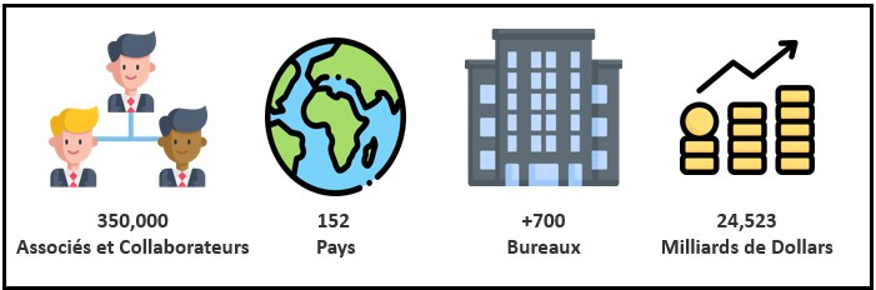
\includegraphics[scale=0.5,height=5cm]{EYGlobal.png}
     \caption{EY Global}
\end{figure}

\hspace{0.5cm}{EY est une entreprise de premier plan à l'échelle mondiale évoluant dans le domaine d’assurance, de fiscalité, de transaction, et de conseil. EY bénéficie d'une équipe mondiale en expansion constante.  }      
     \subsection{AMC EY Tunisie}

\hspace{0.5cm}Établie sur le territoire depuis 1987, AMC EY Tunisie se positionne comme l’une des pionnières dans le domaine des services professionnels du pays. Elle fait partie de la région EMEIA et compte plus de 1000 employés avec plus de 900 consultants en service de conseil. Grâce à plus de 620 missions réalisées annuellement, l’entreprise a atteint un chiffre d’affaires de 50 Millions de dinars tunisiens en 2022 avec plus de 50\% réalisées auprès de clients internationaux.

\begin{figure}[H]
     \centering
     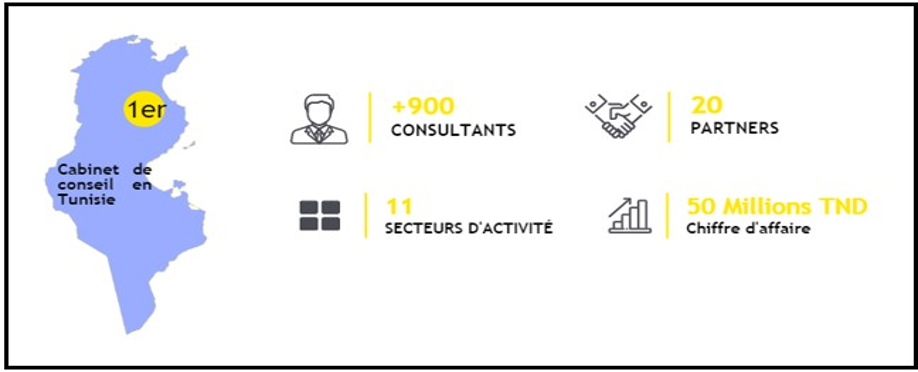
\includegraphics[scale=2,height=5cm]{AMCEYTunisia.png}
     \caption{AMC EY Tunisie}
\end{figure}

\hspace{0.5cm}EY Tunisie intervient dans différents secteurs économiques en Tunisie, notamment dans le secteur des technologies de l’information et de la communication, méritant la confiance tant du secteur public local (ministères, agences de développement local) que du secteur privé grâce à la proposition de solutions adaptées et pertinentes.

\subsection{Services proposés par EY Tunisie}
\hspace{0.5cm}
\hspace{0.5cm}EY Tunisie structure son offre autour de quatre grands métiers complémentaires qui permettent à l’entreprise de répondre aux besoins variés de ses clients résumés dans le tableau suivant:
\begin{figure}[H]
     \centering
     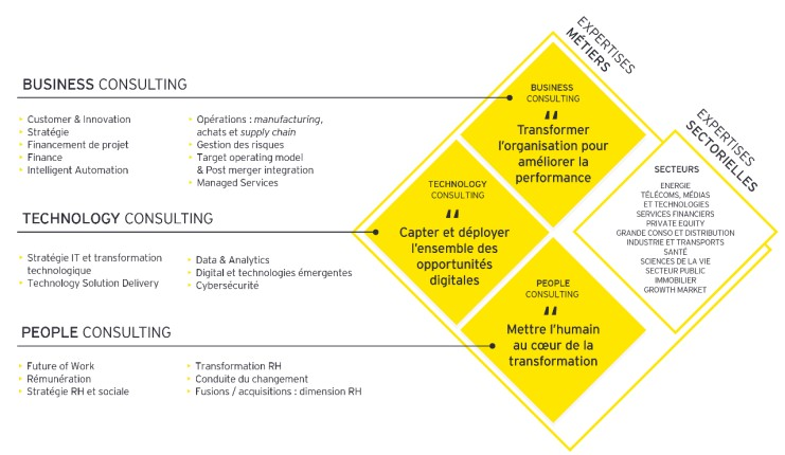
\includegraphics[scale=3,height=8cm]{ServiceEY2.png}
     \caption{Services EY Tunisie}
\end{figure}

\begin{table}[H]
\centering
\renewcommand{\arraystretch}{1.5}
\begin{tabularx}{\textwidth}{|p{2.5cm}|X|}
\hline
\thead{\textbf{Service}} & \textbf{\thead{Description}} \\
\hline
\textbf{Conseil} & EY aide ses clients à créer de la valeur à long terme pour toutes les parties prenantes. En s’appuyant sur les données et la technologie, ses services et ses solutions orientent les clients et les aident à prendre des décisions sur le plan stratégique et opérationnel afin de parvenir favorablement à leurs attentes. \\
\hline
\textbf{Audit} & EY fournit des renseignements et cherche à offrir aux clients (investisseurs) la meilleure gestion et l’adéquate structuration de ses rapports et de ses opérations dans le but d’améliorer voire de valoriser leurs tâches et d’accroître leurs opportunités envers les autres entreprises. \\
\hline
\textbf{Fiscalité et droit (Tax)} & EY possède une expertise en matière d’impôt sur les sociétés, d’impôt international, d’impôt sur les transactions et de ressources humaines, de conformité et de déclaration, et d’impôt statutaire. \\
\hline
\textbf{Stratégies et Transactions} & EY aide ses clients à surmonter la crise et à stabiliser leurs activités à court terme. EY aide également les entreprises à surmonter les ralentissements et à se préparer à la reprise, ou à regarder au-delà pour permettre la transformation par le biais de la stratégie d’entreprise, des transactions, des fusions et acquisitions et des désinvestissements. \\
\hline
\end{tabularx}
\caption{Services professionnels d’EY Tunisie}
\end{table}

\vspace{0.5cm}
\subsection{Présentation du sous service line Technology Strategy \& Transformation:}

\hspace{0.5cm}Le département \textbf{« Technology Strategy \& Transformation »} qui fait partie du service line Consulting occupe une position centrale dans la transformation d'entreprise et propose des possibilités d'optimisation des rendements, de supervision des risques et de promotion de l’innovation des entreprises.

\hspace{0.5cm}En s'appuyant sur une gamme diversifiée de projets technologiques, la division \textbf{« Technology Strategy \& Transformation »} offre à ses clients la possibilité d'améliorer leurs pratiques et d'acquérir un avantage compétitif. L’équipe offre cinq (5) principales activités pour cinq (5) secteurs intersectoriels, comme l’illustre la figure ci-dessous.
\begin{figure}[H]
     \centering
     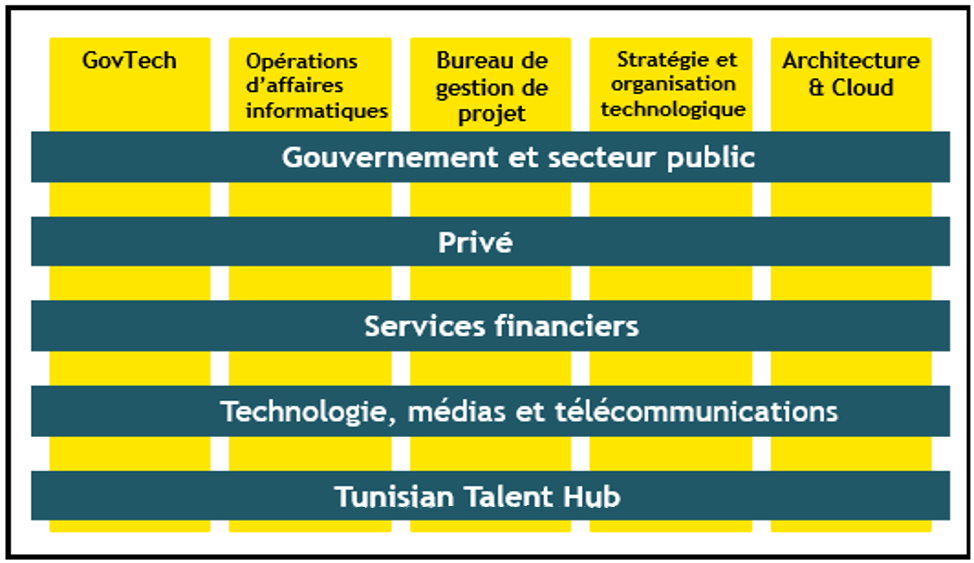
\includegraphics[scale=1.5,height=6cm]{TechTransfo.png}
     \caption{Les activités de la division « Technology Strategy \& Transformation »}
\end{figure}



\section{Présentation du projet}

\vspace{0.5cm}

\subsection{Cadre du projet}
\hspace{0.5cm}Notre projet s'inscrit dans le cadre du stage de fin d'études pour l'obtention du Diplôme National d'Ingénieur en Informatique, réalisé au sein du cabinet EY Tunisie. Il s'inscrit dans une dynamique de transformation numérique des services publics, 
portée par l'adoption des \textbf{Digital Public Infrastructures (DPI)}  et des \textbf{Digital Public Goods (DPG)}. Cette démarche rejoint plusieurs initiatives menées dans des pays francophones, où l'implémentation de 
solutions DPI/DPG bénéficie du soutien de bailleurs de fonds internationaux, dans une strategie de transformation vers infrastructure numérique publique mutualisée et réutilisable au-delà d'un seul programme ou d'un seul pays.\subsection{Contexte du projet}

\hspace{0.5cm}La transformation numérique des administrations publiques s'appuie aujourd'hui sur les \textit{Digital Public Infrastructures} (DPI) et les \textit{Digital Public Goods} (DPG), qui favorisent le développement de services publics numériques interopérables, sécurisés et accessibles. Dans ce contexte, \textit{OpenG2P} constitue un Digital Public Good dédié à la gestion des programmes de protection sociale, en couvrant l'ensemble du cycle de vie des prestations, depuis l'enregistrement des bénéficiaires jusqu'à la distribution des aides.

\hspace{0.5cm}C'est dans cette dynamique que s'inscrit notre projet, réalisé au sein d'EY Tunisie. Il consiste à concevoir et développer un moteur intelligent de détection des risques et des fraudes intégré à la plateforme OpenG2P, afin de renforcer la fiabilité et la transparence des programmes de protection sociale. Une étude préalable de l'architecture et du fonctionnement de la plateforme a permis d'identifier plusieurs limites en matière de détection de la fraude, qui constituent la problématique abordée dans ce mémoire.

\subsection{Problématique}
\hspace{0.5cm}Les programmes de protection sociale gèrent chaque année des flux financiers considérables destinés aux populations vulnérables. Cependant, selon la Banque mondiale, \textbf{jusqu'à 27\% de ce budget} est perdu à cause de la fraude et des erreurs de ciblage\cite{BM_Sourcebook2020}. Les principaux problèmes identifiés sont les suivants:

\begin{itemize}
    \item \textbf{La fraude prend des formes variées et évolutives:} faux bénéficiaires, ménages fictifs, identités partagées, manipulation de paiements.
    \item \textbf{Les contrôles actuels} \textbf{interviennent après le versement:} quand l'argent a déjà quitté les caisses de l'État.
    \item \textbf{Les vérifications manuelles} sont lentes, coûteuses, et ne couvrent qu'un échantillon limité.
    \item \textbf{Les règles de contrôle figées} ne détectent que les fraudes connues et ne s'adaptent pas aux nouvelles tactiques.
    \item \textbf{Les solutions commerciales} existantes sont \textbf{coûteuses, opaques, et incompatibles} avec la philosophie open-source d'OpenG2P.
\end{itemize}


\hspace{0.5cm}Il devient donc indispensable de disposer d'une solution intelligente, proactive et explicable, capable de détecter la fraude \textbf{avant} le versement.

\subsection{Objectif du projet}
\hspace{0.5cm}Face à ces constats, notre projet a pour ambition de transformer fondamentalement la manière dont les programmes de protection sociale luttent contre la fraude. L'objectif n'est pas simplement de détecter des cas suspects, mais de \textbf{changer le paradigme} : passer d'un système réactif, qui découvre la fraude après le versement, à un système intelligent qui la prévient avant qu'elle ne cause des dégâts. Pour y parvenir, nous avons structuré notre travail autour de cinq objectifs principaux :

\begin{itemize}[label=\textbullet]
    \item \textbf{Détection proactive :} identifier les bénéficiaires à risque avant le versement, au moment même de leur enregistrement dans le système.
    \item \textbf{Analyse multi-couches :} croiser plusieurs signaux complémentaires règles métier, apprentissage automatique, comportements inhabituels et liens entre bénéficiaires pour ne laisser aucun angle mort.
    \item \textbf{Explicabilité des décisions :} accompagner chaque alerte d'une explication claire en français, permettant à un agent social de comprendre et de justifier pourquoi un cas est signalé.
    \item \textbf{Amélioration continue :} créer un système qui apprend des retours des enquêteurs et devient plus performant au fil du temps.
    \item \textbf{Accessibilité et intégration :} offrir une solution 100\% open-source, gratuite et intégrée directement à la plateforme OpenG2P que les gouvernements utilisent déjà.
\end{itemize}


\subsection{Étude de l'existant: la plateforme OpenG2P}
\hspace{0.5cm}Avant de proposer une solution, il est essentiel de comprendre comment fonctionne la plateforme sur laquelle elle sera intégrée. Nous avons donc mené une étude approfondie d'OpenG2P, son architecture, ses modules, et ses processus métier, afin d'identifier précisément où se situent les faiblesses face à la fraude.

\subsubsection{Présentation d'OpenG2P}
\begin{figure}[H]
            \centering
            
\includegraphics[scale=1.5,height=5cm]{OpenG2P.png}
          \caption{Logo de OpenG2P}

          \end{figure}
\hspace{0.5cm}\textbf{OpenG2P} est une plateforme open-source bâtie sur Odoo 17, conçue pour centraliser la gestion des programmes de protection sociale. Elle est déployée dans plusieurs pays (Kenya, Malawi, Sierra Leone etc) et couvre l'ensemble du cycle de vie d'un programme social, depuis l'enregistrement des bénéficiaires jusqu'au versement des aides. La plateforme s'organise autour de plusieurs modules interconnectés:
\begin{figure}[H]
            \centering
            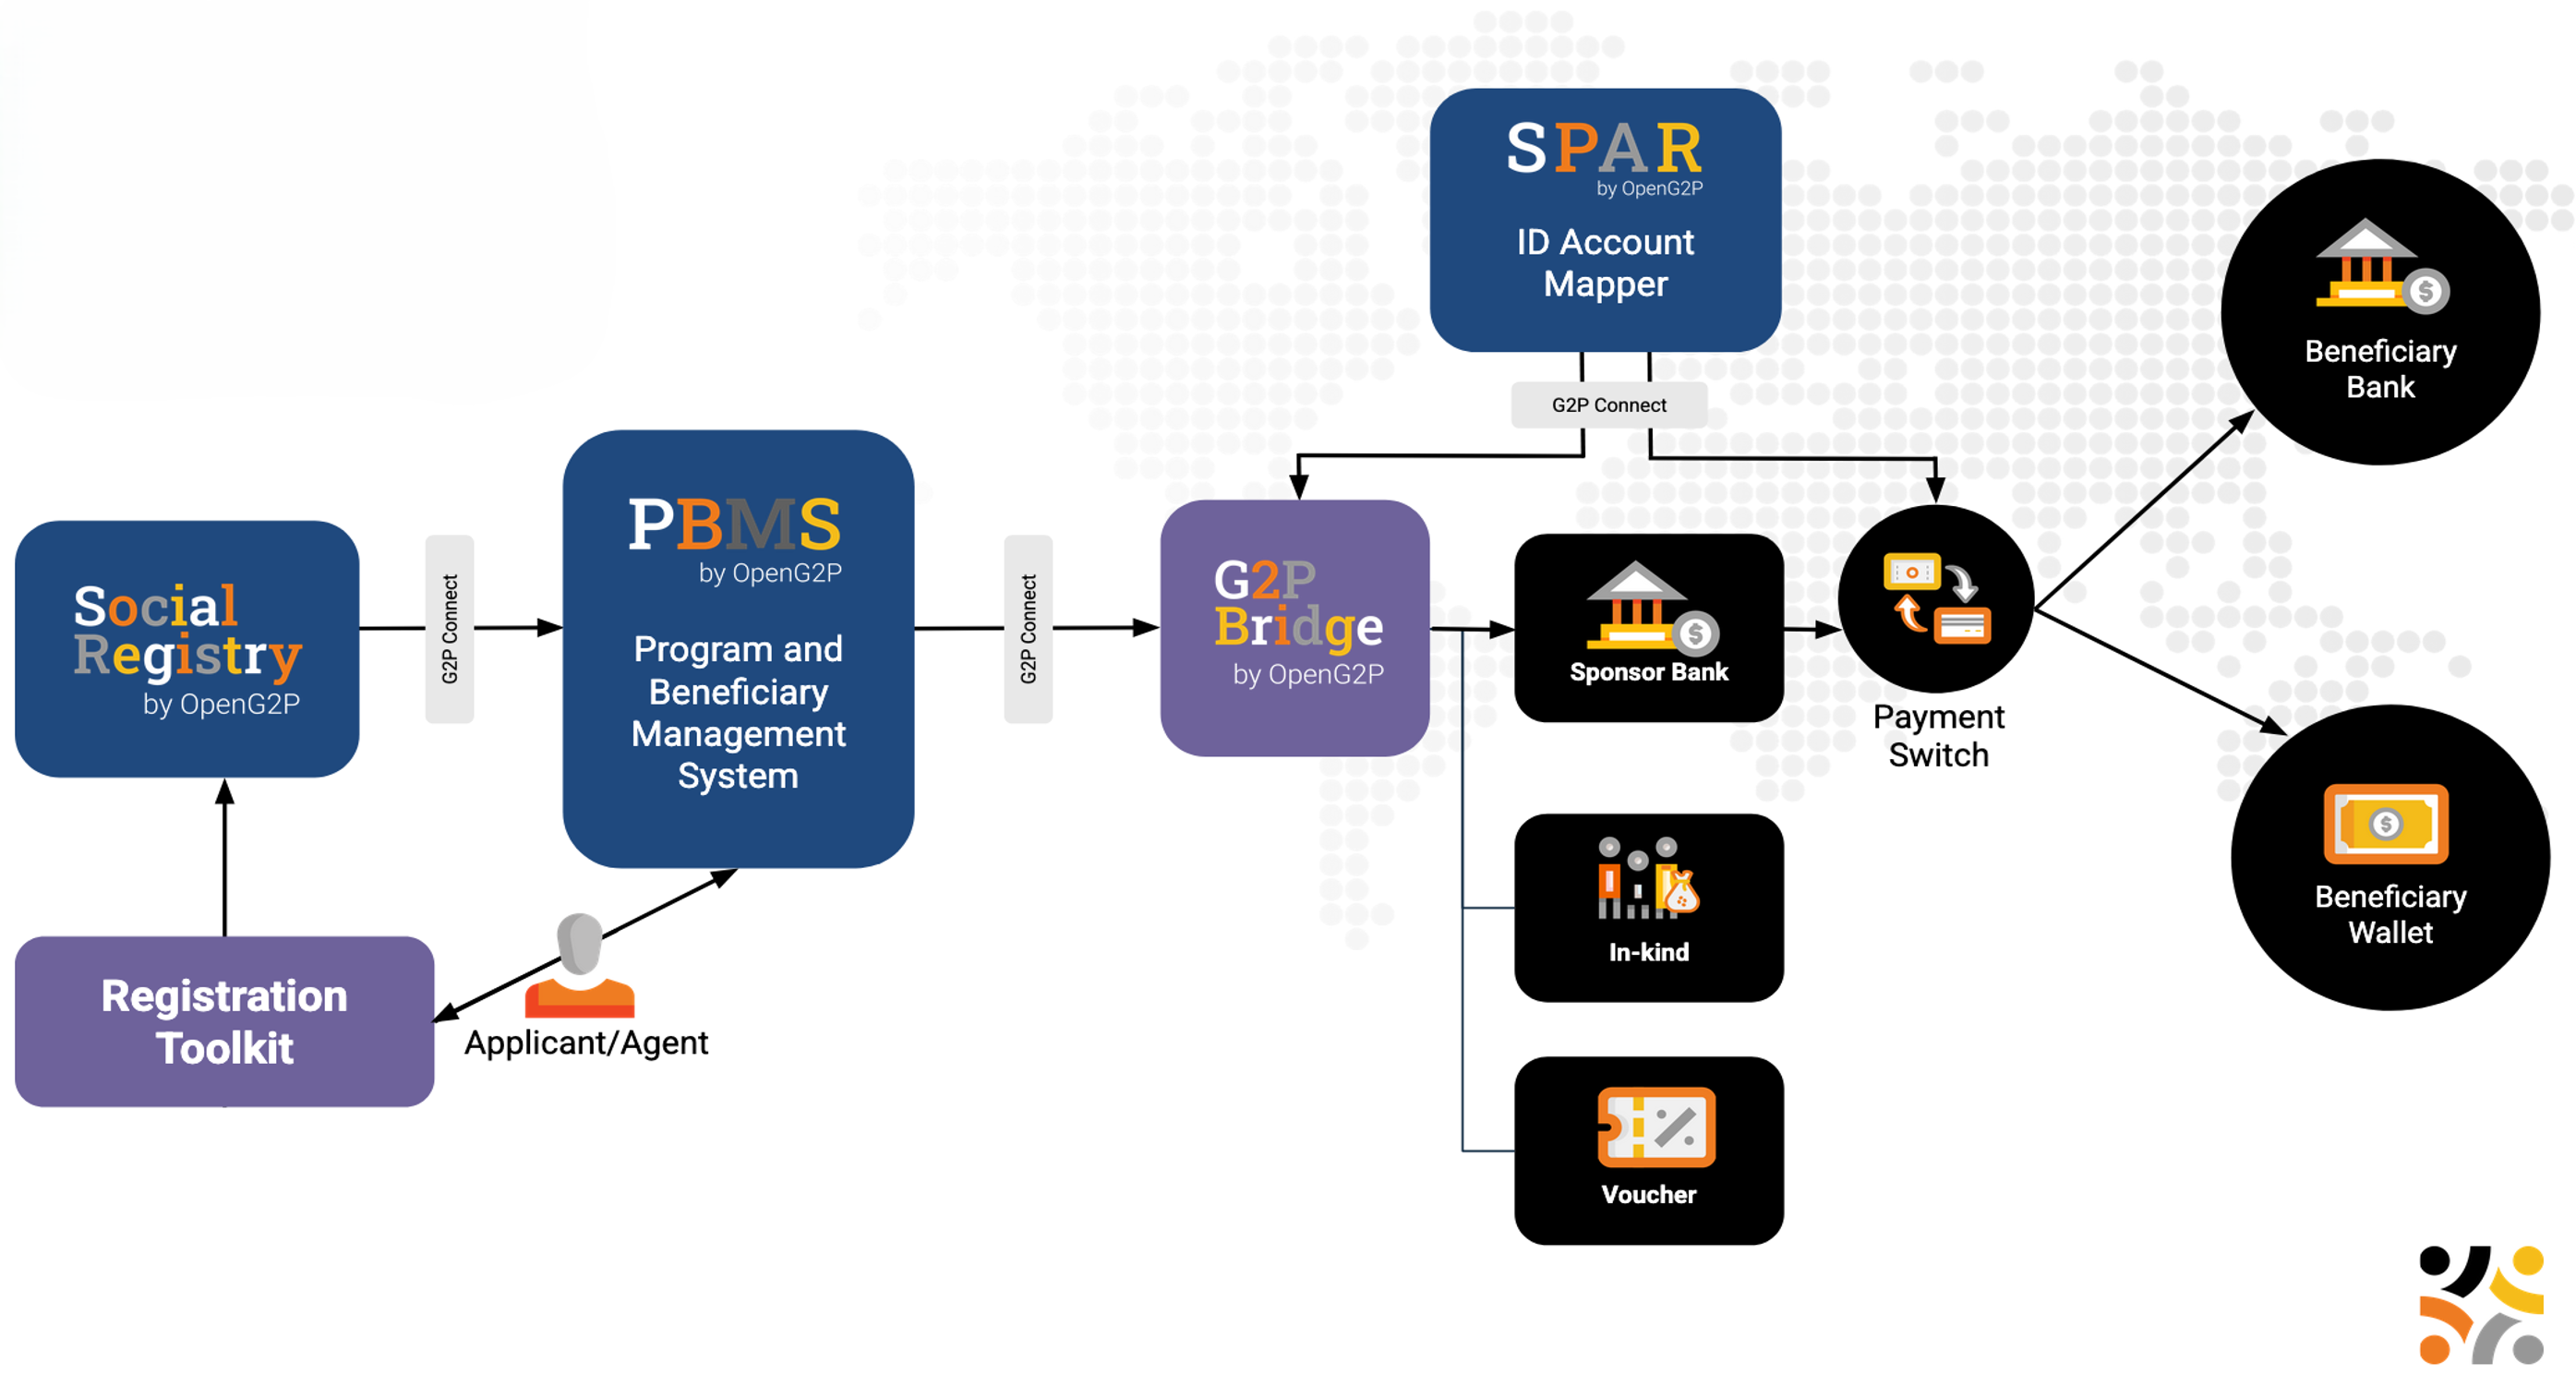
\includegraphics[scale=1.5,height=10cm]{AFOpenG2P.png}
          \caption{Architecture fonctionelle de OpenG2P}
          \end{figure}

\begin{itemize}[label=\textbullet]
    \item \textbf{Registre social (Social Registry)}: base de données centralisée des bénéficiaires avec leurs informations personnelles, démographiques et socio-économiques
    \item \textbf{Gestion des programmes (PBMS)}: définition des programmes d'aide, organisation des cycles de versement (trimestriels, mensuels)
    \item \textbf{Droits et paiements(SPAR)}: calcul automatisé des montants dus à chaque bénéficiaire et suivi de chaque versement
    \item \textbf{Données transactionnelles(G2P Bridge)}: registre des coordonnées téléphoniques et bancaires utilisées pour les transferts
    \item \textbf{Groupes et ménages}: gestion des liens familiaux et des regroupements de bénéficiaires
\end{itemize}

\subsubsection{Processus actuel dans OpenG2P et les limites face au risque de fraude}
\hspace{0.5cm}Le processus de contrôle anti-fraude dans OpenG2P repose actuellement sur un système minimal: quelques vérifications manuelles effectuées par les agents sociaux lors de l'enregistrement des bénéficiaires, complétées par des audits post-versement sur un échantillon limité. Aucun moteur automatisé de détection n'est intégré à la plateforme.
 
\hspace{0.5cm}Afin de mieux comprendre les limites du système actuel, nous présentons ci-dessous une analyse des mécanismes de contrôle existants.
 
\hspace{0.5cm}La Figure 1.6 illustre le processus actuel de vérification dans OpenG2P, où l'agent social consulte manuellement les fiches des bénéficiaires et effectue des contrôles ponctuels sans outil d'aide à la décision :
 
\begin{figure}[H]
    \centering
    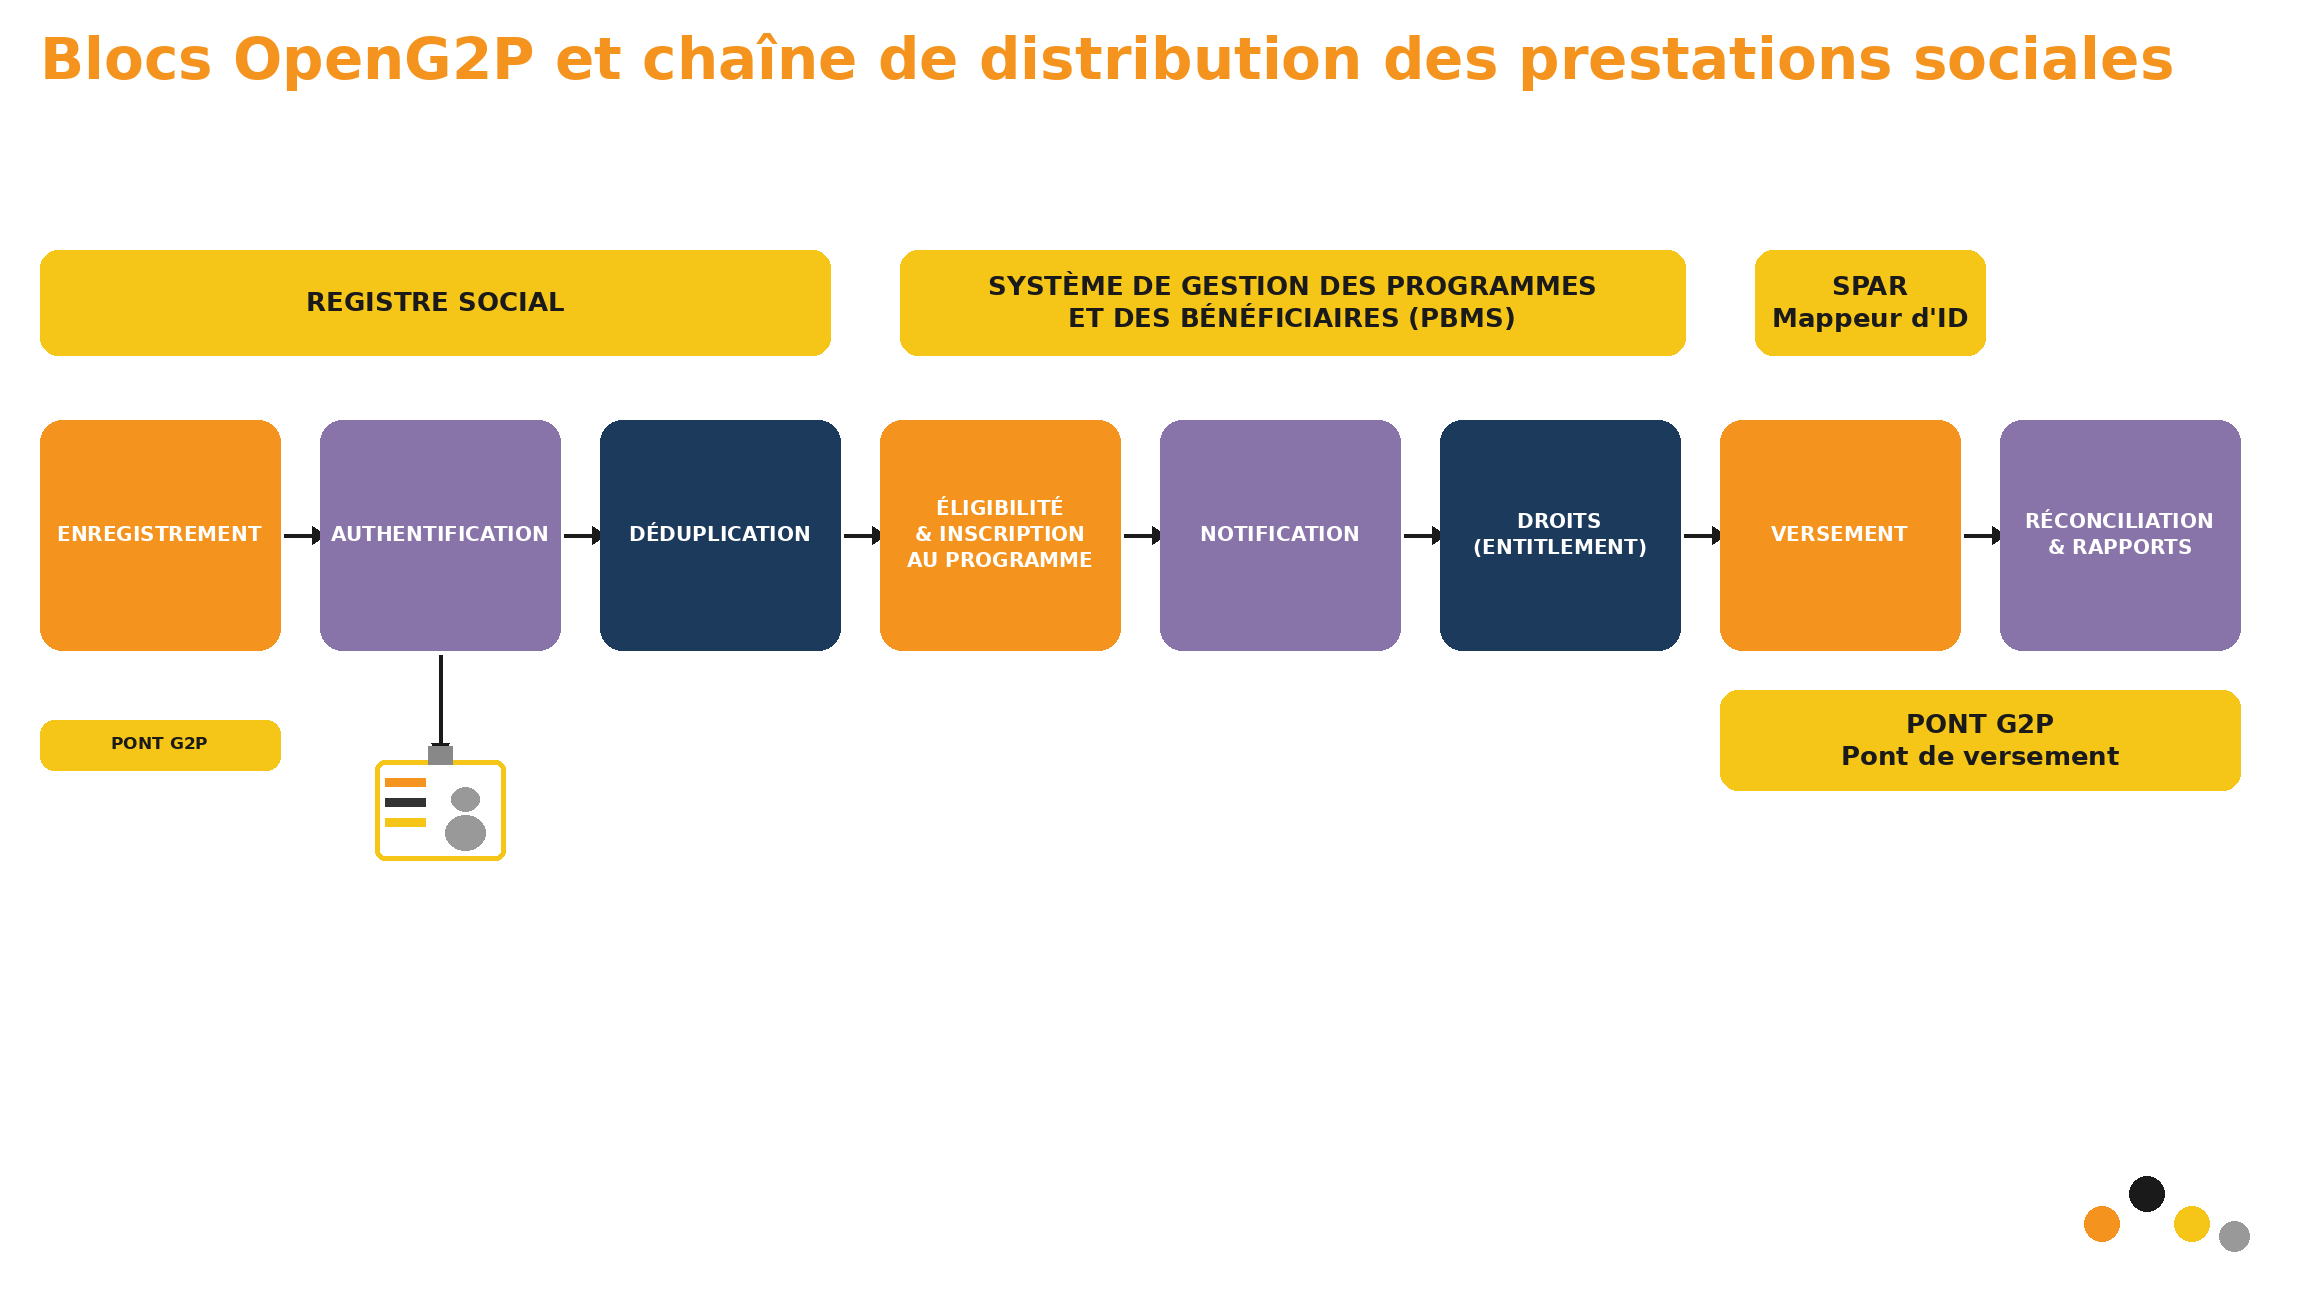
\includegraphics[width=0.85\textwidth]{ProcessusOpeng2p.png}
    \caption{Processus actuel dans OpenG2P et les zones de vulnérabilité à la fraude}
    \label{fig:processus_openg2p}
\end{figure}

\hspace{0.5cm}Comme le montre cette figure, \textbf{aucun mécanisme de détection automatique} n'intervient entre l'enregistrement et le versement. La fraude peut s'infiltrer à chaque étape sans être détectée, et les contrôles manuels post-versement ne couvrent qu'une fraction des cas.
 


\section{Choix méthodologique et conceptuel}

\subsection{Méthodologie de conception}
\hspace{0.5cm}Pour la conception de ce projet, nous avons adopté le langage de modélisation \textbf{UML} afin de représenter les différentes vues du système de manière standardisée. Nous avons retenu quatre diagrammes : cas d'utilisation, classes, séquence et déploiement, qui permettent de couvrir respectivement les interactions, la structure, le flux de scoring et l'architecture Docker du système.

\subsection{Méthodologie adoptée}
\hspace{0.5cm}La nature exploratoire d'un projet de data science où les données évoluent, les modèles doivent être comparés et les hypothèses remises en question impose une méthodologie flexible. Nous avons donc adopté la méthode \textbf{SCRUM}, un cadre agile structuré en sprints de 1 à 2 semaines, permettant de livrer des incréments fonctionnels et d'intégrer les retours d'EY Tunisie de manière continue.

\subsubsection{Comparaison entre les méthodologies traditionnelles et agiles}

\begin{table}[H]
\centering
\begin{tabular}{|p{4.5cm}|p{5cm}|p{5cm}|}
\hline
\thead{Critère} & \thead{Traditionnelle} & \thead{Agile} \\
\hline
Approche & Linéaire et séquentielle & Itérative et incrémentale \\
\hline
Exigences & Figées au départ & Évolutives \\
\hline
Changement & Difficile et coûteux & Flexible et intégré \\
\hline
Client & Impliqué au début et à la fin & Impliqué en continu \\
\hline
Livraison & Une seule fois à la fin & Fréquente (cycles courts) \\
\hline
Risques & Identifiés tardivement & Maîtrisés en continu \\
\hline
\end{tabular}
\caption{Méthodologies Traditionnelles vs Agiles}
\label{tab:comparaison_methodo}
\end{table}

\subsection{Pilotage du projet}
\hspace{0.5cm}Le projet a été organisé en six phases : cadrage, conception, génération de données, modélisation ML, intégration et tests. L'équipe SCRUM est composée comme suit :\\

\noindent\textbf{Product Owner:} EY Tunisie \\
\textbf{Scrum Master:} [Cyrine Garram, Mariem Abcha] \\
\textbf{Équipe de développement:} [Halim Trabelsi]

\subsubsection{Les rôles de la méthodologie Scrum}

\hspace{0.5cm}La méthode \textbf{Scrum} repose sur trois rôles principaux :

\begin{description}
    \item[\textbf{Product Owner:}] Représente les besoins fonctionnels du projet, définit les priorités, gère le \textit{Product Backlog} et valide les livrables à la fin de chaque sprint.
    \item[\textbf{Scrum Master:}] Garantit l'application de la méthodologie Scrum, facilite les échanges entre les membres de l'équipe et veille à la résolution des obstacles rencontrés.
    \item[\textbf{Équipe projet:}] Réunit les membres chargés de la conception, du développement, des tests et de l'intégration de la solution afin d'atteindre les objectifs définis pour chaque sprint.
\end{description}

\subsubsection{Les concepts de base de la méthodologie Scrum}

\hspace{0.5cm}La méthode \textbf{Scrum} s'appuie sur plusieurs concepts fondamentaux qui permettent d'organiser et de piloter efficacement le développement du projet :

\begin{description}
    \item[\textbf{Backlog produit :}] Il s'agit de la liste des besoins, des fonctionnalités et des objectifs du projet, classés par ordre de priorité. Ce backlog évolue tout au long du projet en fonction des besoins et des retours des parties prenantes.

    \item[\textbf{Sprint Backlog :}] Il correspond à l'ensemble des tâches sélectionnées à partir du backlog produit pour être réalisées au cours d'un sprint donné.

    \item[\textbf{Sprint :}] Il s'agit d'une période de travail de durée limitée, généralement comprise entre une et quatre semaines, durant laquelle l'équipe développe un incrément fonctionnel du produit.

    \item[\textbf{Mêlée quotidienne (\textit{Daily Scrum}) :}] C'est une courte réunion quotidienne permettant de suivre l'avancement des travaux, d'identifier les difficultés rencontrées et de coordonner les actions à entreprendre.

    \item[\textbf{Incrément :}] Il représente le résultat obtenu à la fin d'un sprint. Chaque incrément doit constituer une version fonctionnelle et exploitable du produit, apportant une valeur ajoutée au projet.
\end{description}

\hspace{0.5cm}La Figure~\ref{fig:scrum-process} illustre le déroulement général du processus Scrum.

\begin{figure}[H]
    \centering
    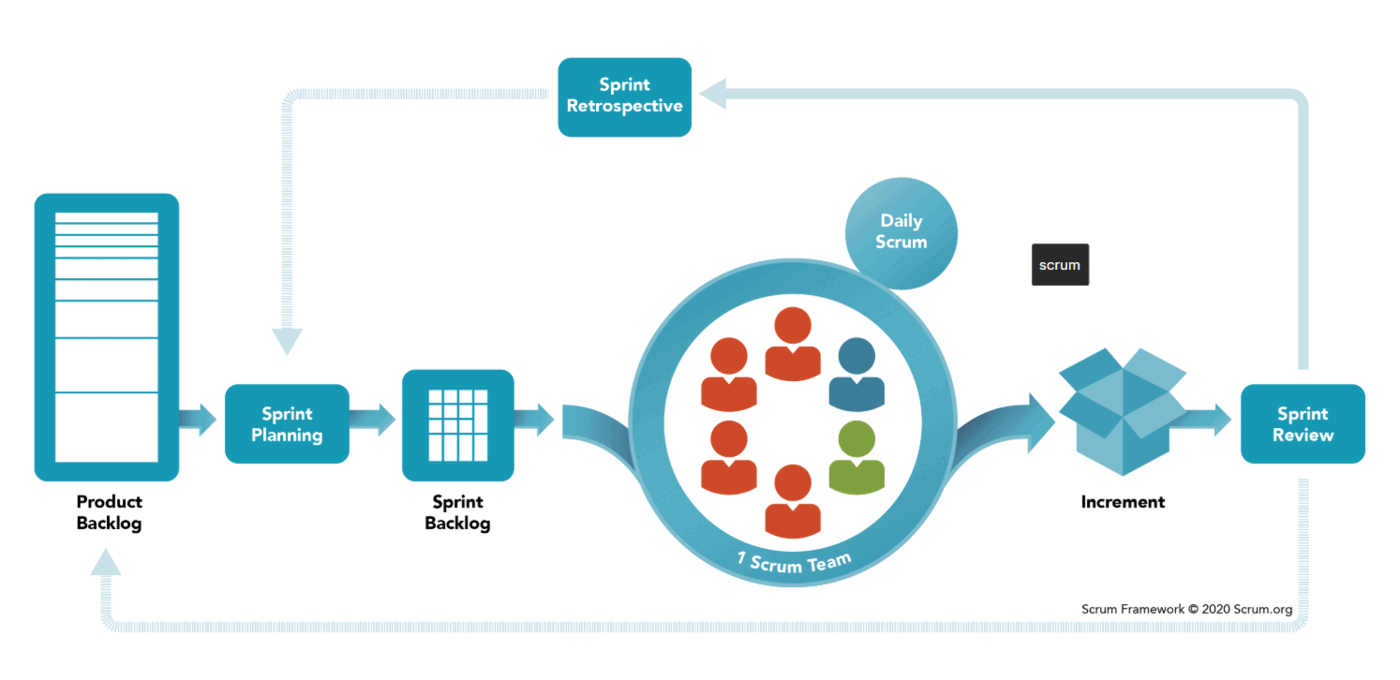
\includegraphics[width=0.9\textwidth]{scrum_process.png}
    \caption{Déroulement général du processus Scrum}
    \label{fig:scrum-process}
\end{figure}



\section{Diagramme de Gantt}
\hspace{0.5cm}Le diagramme de Gantt ci-dessous présente la planification temporelle du projet, découpée en phases et en sprints sur la durée du stage. La Figure~\ref{fig:gantt} illustre cette répartition en utilisant les mois comme unité de temps.

\begin{figure}[H]
    \centering
     \includegraphics[width=0.98\textwidth]{gantt.png}
    \caption{Diagramme de Gantt du projet}
    \label{fig:gantt}
\end{figure}

\noindent\textbf{Les principales phases du projet sont les suivantes :}

\begin{description}
    \item[\textbf{Cadrage et recherche:}] Cette première phase a consisté à analyser le contexte du projet, identifier les besoins de l'entreprise, étudier OpenG2P ainsi que les travaux existants relatifs à la détection de fraude.

    \item[\textbf{Conception et architecture:}] Cette étape a permis de définir l'architecture de la solution, les technologies à utiliser ainsi que les différents modules composant le moteur intelligent.

    \item[\textbf{Préparation du jeu de données:}] Cette phase a été consacrée à l'identification des scénarios de fraude, à la conception des caractéristiques (\textit{features}) et à la génération d'un jeu de données synthétique destiné à l'entraînement et à l'évaluation des modèles.

    \item[\textbf{Développement du moteur intelligent:}] Cette étape correspond à l'implémentation du moteur de détection de fraude, incluant le moteur de règles, les modèles de Machine Learning, l'analyse des graphes et le calcul du score de risque.

    \item[\textbf{Intégration à OpenG2P :}] Cette phase a consisté à intégrer la solution développée au sein de la plateforme OpenG2P, à assurer la communication entre les différents composants et à valider le bon fonctionnement de l'ensemble.

    \item[\textbf{Rédaction du rapport et livraison :}] La dernière phase a porté sur la rédaction du mémoire, la préparation de la soutenance, la finalisation des livrables et la validation finale du projet.
\end{description}

\section*{Conclusion}
\hspace{0.5cm}Ce chapitre a posé les fondations du projet: après avoir présenté le cadre institutionnel, étudié les lacunes d'OpenG2P et du marché, et défini nos objectifs, nous avons adopté une méthodologie SCRUM adaptée à la nature itérative d'un projet de data science. Le chapitre suivant sera consacré à l'\textbf{état de l'art}, où nous examinerons les techniques de détection de fraude dans la littérature scientifique afin de justifier les choix techniques de notre solution.


\chapter{État de l'art}

\section*{Introduction}
\hspace{0.5cm}Avant de détailler la conception et la réalisation de notre solution, il est essentiel de poser les bases théoriques sur lesquelles elle repose. Ce chapitre a pour objectif de présenter les notions fondamentales nécessaires à la compréhension du projet et d'examiner les techniques existantes dans la littérature scientifique pour la détection de fraude.

\section{Définitions et concepts clés}

\hspace{0.5cm}Il est indispensable de définir le vocabulaire et les notions fondamentales qui seront mobilisés tout au long de ce rapport. Cette section a pour but de rendre le reste du document accessible à tout lecteur, y compris ceux qui ne sont pas familiers avec les domaines de l'intelligence artificielle ou de l'analyse de données.

% ═══════════════════════════════════════════════════════════
% FRAUDE ET PROTECTION SOCIALE
% ═══════════════════════════════════════════════════════════

\subsection{Concepts liés à la fraude et à la protection sociale:}

\begin{itemize}[label=\textbullet]

    \item \textbf{Programme G2P (Government-to-Person):} mécanisme par lequel un gouvernement verse des aides financières directement aux citoyens éligibles (allocations familiales, bourses, aides alimentaires). C'est le contexte métier de notre projet.

    \item \textbf{Détection de fraude:} ensemble des méthodes permettant d'identifier des comportements malhonnêtes ou irréguliers dans un système. Dans notre cas, il s'agit de repérer les bénéficiaires qui tentent de recevoir indûment des aides sociales.
    
    \item \textbf{Protection sociale:} ensemble des politiques et programmes publics visant à
    réduire la pauvreté et la vulnérabilité des populations, à travers des transferts monétaires,
    des aides alimentaires ou un accès facilité aux services essentiels (santé, éducation). Les
    programmes de protection sociale constituent le terrain d'application de notre système de
    détection de fraude.
    
    \item \textbf{Bénéficiaire:} individu ou ménage inscrit à un ou plusieurs programmes de protection sociale et destinataire des prestations versées. C'est l'entité sur laquelle porte l'analyse de risque de fraude dans notre système.
    
    \item \textbf{Fraude sociale:} manipulation intentionnelle des informations ou des processus
    d'un programme social dans le but d'obtenir un avantage indu. Elle se distingue de l'erreur
    involontaire (déclaration erronée non intentionnelle) par la présence d'une intention de
    tromper le système. Plusieurs typologies sont couvertes par notre moteur de règles~:
    \begin{itemize}[label=\textendash]
        \item \textbf{\textit{inscription multiple (multi-enrollment)}}: un même bénéficiaire s'inscrit
        à un nombre anormalement élevé de programmes cumulables,;
        \item \textbf{\textit{usurpation d'identité (identity fraud)}}: utilisation d'une identité
        fictive ou empruntée, souvent révélée par le partage d'un même numéro de téléphone ou
        compte bancaire entre plusieurs bénéficiaires.
        \item \textbf{\textit{ménage fantôme (ghost household)}}: déclaration d'un ménage fictif ou
        surdimensionné pour augmenter le montant de l'aide perçue.
        \item \textbf{\textit{sous-déclaration de revenus (income underreporting)}}: dissimulation du
        revenu réel afin de paraître éligible à un programme destiné aux ménages les plus
        pauvres.
        \item \textbf{\textit{manipulation des paiements (payment manipulation)}}: anomalies
        volontaires dans le cycle de versement (paiements dupliqués, écarts injustifiés entre
        montant émis et montant perçu).
        \item \textbf{\textit{fraude en réseau (collusion)}}: coordination entre plusieurs bénéficiaires
        (partage de coordonnées bancaires ou téléphoniques) pour multiplier les gains
        frauduleux, détectable par analyse de graphe.
    \end{itemize}
    
\end{itemize}

% ═══════════════════════════════════════════════════════════
% IA ET DONNÉES
% ═══════════════════════════════════════════════════════════

\subsection{Concepts d'Intelligence Artificielle et Machine Learning}

\hspace{0.5cm}L'intelligence artificielle, et plus précisément le machine learning, 
est au cœur de notre solution. Pour comprendre comment notre système apprend à 
distinguer un bénéficiaire légitime d'un fraudeur, il est nécessaire de maîtriser 
les notions suivantes:

\begin{itemize}[label=\textbullet]

    \item \textbf{Machine Learning (apprentissage automatique):} branche de 
    l'intelligence artificielle où un programme apprend à prendre des décisions 
    à partir d'exemples passés, sans être explicitement programmé pour chaque cas. 
    Le programme identifie des régularités dans les données et les utilise pour 
    faire des prédictions sur de nouveaux cas.

    \item \textbf{Apprentissage supervisé:} type de machine learning où le modèle 
    apprend à partir d'exemples dont on connaît déjà la réponse (par exemple : 
    « ce bénéficiaire est un fraudeur » ou « ce bénéficiaire est légitime »). Le 
    modèle apprend la relation entre les caractéristiques d'un bénéficiaire et son 
    statut, puis applique cette connaissance aux nouveaux cas.

    \item \textbf{Apprentissage non supervisé:} type de machine learning où le 
    modèle ne dispose pas de réponses connues. Il cherche à identifier des 
    comportements atypiques ou des groupes naturels dans les données, sans savoir 
    à l'avance ce qui est normal ou anormal.

    \item \textbf{Feature engineering (extraction de caractéristiques):} étape qui 
    consiste à transformer les données brutes en variables exploitables par un 
    modèle. Par exemple, à partir du nombre de téléphones partagés et du nombre de 
    comptes bancaires partagés, on calcule un « score de risque réseau » qui 
    résume l'information en un seul chiffre.

    \item \textbf{Data leakage (fuite de données):} erreur dans la construction du 
    modèle où des informations liées à la réponse (le label fraude/légitime) se 
    retrouvent accidentellement dans les données d'entraînement. Le modèle semble 
    alors parfait, mais ses performances sont artificiellement gonflées et ne se 
    reproduisent pas en conditions réelles.

    \item \textbf{Collusion:} forme de fraude collective où plusieurs individus 
    collaborent pour tromper le système — par exemple, en partageant un même 
    compte bancaire ou un même numéro de téléphone pour multiplier les inscriptions.

\end{itemize}

\subsection{Métriques d'Évaluation et Concepts de Validité}

\hspace{0.5cm}Pour évaluer la performance d'un modèle de détection de fraude, 
il est essentiel de comprendre les métriques suivantes, qui permettent de mesurer 
son efficacité et ses limitations :

\begin{itemize}[label=\textbullet]

    \item \textbf{Vrai positif:} cas où le système identifie correctement une 
    transaction ou un bénéficiaire réellement frauduleux comme étant frauduleux.

    \item \textbf{Vrai négatif:} cas où le système identifie correctement une 
    transaction ou un bénéficiaire légitime comme étant non frauduleux.

    \item \textbf{Faux positif:} cas où le système signale un bénéficiaire comme 
    fraudeur alors qu'il est légitime. Un excès de faux positifs surcharge 
    inutilement les enquêteurs et nuit à la confiance envers le système.

    \item \textbf{Faux négatif:} cas où le système laisse passer un vrai fraudeur 
    sans le détecter. C'est la situation la plus coûteuse, car l'argent est versé 
    à une personne qui n'y a pas droit.

    \item \textbf{Accuracy (exactitude):} proportion de prédictions correctes 
    (vrais positifs + vrais négatifs) parmi l'ensemble des prédictions effectuées.
    
    \item \textbf{Précision (precision):} proportion de cas réellement frauduleux 
    parmi tous les cas que le système a prédits comme frauduleux.
    
    \item \textbf{Rappel (recall):} proportion de cas réellement frauduleux que le 
    système a effectivement réussi à détecter parmi tous les cas frauduleux 
    existants.
    
    \item \textbf{F1-score:} moyenne harmonique de la précision et du rappel, 
    offrant une mesure équilibrée de la performance du modèle, surtout lorsque les 
    classes sont déséquilibrées (comme c'est souvent le cas en détection de fraude).

    \item \textbf{AUC-ROC (Area Under the Receiver Operating Characteristic Curve):} 
    métrique d'évaluation qui mesure la capacité d'un modèle à distinguer les 
    fraudeurs des légitimes, sur une échelle de 0 à 1. Un AUC de 0.5 signifie que 
    le modèle ne fait pas mieux que le hasard ; un AUC de 1.0 signifie une 
    détection parfaite. Dans la pratique, un AUC supérieur à 0.85 est considéré 
    comme bon.

\end{itemize}

\subsection{Explicabilité et génération d'explications}

\hspace{0.5cm}Un système de détection de fraude ne peut être utile que s'il est compréhensible par ses utilisateurs. Un agent social doit pouvoir expliquer à un bénéficiaire pourquoi son dossier a été signalé. C'est le rôle de l'explicabilité :

\begin{itemize}[label=\textbullet]

    \item \textbf{XAI (Explainable Artificial Intelligence):} domaine de l'intelligence artificielle qui vise à rendre les décisions des modèles compréhensibles par des humains. Plutôt qu'une « boîte noire » qui dit simplement « fraude détectée », un système explicable indique \textit{pourquoi} : quels facteurs ont pesé dans la décision.

    \item \textbf{SHAP (SHapley Additive exPlanations):} méthode d'explicabilité qui attribue à chaque caractéristique du bénéficiaire une contribution précise au score final. Par exemple : « le partage de téléphone avec 4 autres bénéficiaires a augmenté le score de risque de +0.15 ». SHAP est fondé sur la théorie des jeux (valeurs de Shapley) et constitue aujourd'hui le standard de l'industrie.

    \item \textbf{LLM (Large Language Model):} modèle d'intelligence artificielle capable de comprendre et de générer du texte en langage naturel. Dans notre projet, nous utilisons Mistral (via Ollama) pour transformer les facteurs SHAP et les drapeaux de règles en une \textbf{explication rédigée en français}, compréhensible par un agent social non-technique.

    \item \textbf{RAG (Retrieval-Augmented Generation):} technique qui enrichit la réponse d'un LLM en lui fournissant des documents pertinents avant la génération. Dans notre contexte, le LLM reçoit les facteurs SHAP, les règles déclenchées et le score du bénéficiaire comme contexte, ce qui lui permet de produire une explication précise et fondée sur des faits réels, et non sur des connaissances génériques.

\end{itemize}

% ═══════════════════════════════════════════════════════════
% ANALYSE DE GRAPHE
% ═══════════════════════════════════════════════════════════

\subsection{Analyse de graphe et détection de réseaux}

\hspace{0.5cm}La fraude n'est pas toujours l'acte d'un individu isolé. Souvent, plusieurs personnes collaborent en partageant des ressources (téléphones, comptes bancaires). L'analyse de graphe permet de révéler ces réseaux invisibles:

\begin{itemize}[label=\textbullet]

    \item \textbf{Graphe:} structure mathématique composée de \textbf{nœuds} (les entités — ici, les bénéficiaires) et d'\textbf{arêtes} (les relations entre eux — ici, le partage d'un téléphone ou d'un compte bancaire). Si deux bénéficiaires partagent le même numéro de téléphone, une arête les relie.

    \item \textbf{Détection de communautés:} technique qui identifie des groupes de nœuds fortement connectés entre eux. Une communauté dense de 5 à 15 bénéficiaires partageant plusieurs téléphones et comptes bancaires est un signal fort de fraude organisée.

    \item \textbf{Centralité (PageRank):} mesure d'importance d'un nœud dans un réseau. Un bénéficiaire très connecté (lié à de nombreux autres bénéficiaires suspects) obtient un score de centralité élevé. Notre solution utilise l'algorithme PageRank, le même que celui inventé par Google pour classer les pages web adapté au contexte de la fraude sociale.

\end{itemize}

\subsection{Modèles de Machine Learning et Architectures de Détection}

\hspace{0.5cm}Au-delà des principes fondamentaux du machine learning, plusieurs 
modèles et architectures spécialisés ont été développés pour traiter les problèmes 
complexes comme la détection de fraude. Voici les plus importants:

\begin{itemize}[label=\textbullet]

    \item \textbf{XGBoost (eXtreme Gradient Boosting):} algorithme qui combine 
    des centaines d'arbres de décision simples, chacun corrigeant les erreurs du 
    précédent, pour obtenir des prédictions très précises. C'est le modèle principal 
    retenu dans notre solution en raison de sa performance exceptionnelle sur 
    les données déséquilibrées.

    \item \textbf{Random Forest (forêt aléatoire):} algorithme qui construit 
    plusieurs arbres de décision indépendants et combine leurs prédictions par vote 
    majoritaire. Il est robuste au surapprentissage et sert de modèle de comparaison 
    fiable.

    \item \textbf{Isolation Forest:} algorithme de détection d'anomalies qui isole 
    les comportements atypiques en mesurant leur facilité à se séparer du reste des 
    données. Plus un individu est isolé rapidement, plus il est suspect.

    \item \textbf{Régression logistique:} modèle supervisé qui estime la probabilité 
    qu'un cas appartienne à une classe (fraude ou légitime). Bien que simple, il 
    offre une excellente interprétabilité — chaque coefficient explique directement 
    son impact.

    \item \textbf{Sur-apprentissage (overfitting):} situation où un modèle apprend 
    les détails spécifiques des données d'entraînement au lieu des régularités 
    générales. Un modèle surappris performe parfaitement sur les données vues mais 
    échoue sur les nouvelles.

    \item \textbf{Sous-apprentissage (underfitting):} situation inverse où le modèle 
    est trop simple pour capturer les régularités des données. Un modèle 
    sous-appris performe mal sur l'entraînement et ne généralise pas aux données 
    nouvelles.

    \item \textbf{Validation croisée (cross-validation):} technique qui divise les 
    données en plusieurs sous-ensembles et entraîne le modèle sur chaque combinaison. 
    Elle offre une évaluation robuste et fiable de la performance réelle du modèle.

    \item \textbf{SHAP (SHapley Additive exPlanations):} technique d'interprétabilité 
    basée sur la théorie des jeux qui assigne une « contribution » à chaque feature. 
    Elle garantit que les explications de chaque prédiction sont équitables et 
    théoriquement justifiées.

    \item \textbf{Analyse de réseau et PageRank:} approche qui construit un graphe 
    où les nœuds sont des bénéficiaires et les arêtes représentent des connexions 
    (téléphones ou comptes partagés). PageRank attribue un score de centralité qui 
    révèle les réseaux de fraude organisée.

    \item \textbf{Stacking (méta-apprentissage):} technique qui combine les 
    prédictions de plusieurs modèles en entraînant un méta-modèle pour fusionner les 
    scores optimalement. Elle tire parti des forces de chaque modèle et réduit leurs 
    faiblesses individuelles.

    \item \textbf{Déséquilibre de classes (class imbalance):} problème courant en 
    détection de fraude où les fraudes sont rares (1-5\%) et les données 
    d'entraînement contiennent beaucoup plus d'exemples légitimes. On le résout par 
    des techniques comme SMOTE, l'ajustement des poids de classe, ou l'évaluation 
    sur des métriques appropriées.

    \item \textbf{Calibration du modèle:} processus qui garantit que la probabilité 
    prédite par le modèle (par exemple 0.7) reflète la véritable probabilité empirique 
    de fraude. Un modèle bien calibré fournit des seuils de décision fiables pour 
    les systèmes de production.

\end{itemize}

% ═══════════════════════════════════════════════════════════
% ARCHITECTURE ET PLATEFORME
% ═══════════════════════════════════════════════════════════

\subsection{Architecture et plateforme}

\hspace{0.5cm}Notre solution s'intègre dans un écosystème technique existant. Les termes suivants décrivent les briques d'architecture utilisées:

\begin{itemize}[label=\textbullet]

  \item \textbf{Moteur de règles (Rule Engine):} composant logiciel qui évalue un ensemble de conditions prédéfinies par des experts métier (par exemple :« si le bénéficiaire partage son compte bancaire avec 2 autres personnes, déclencher une alerte »). Les règles sont transparentes, auditables et modifiables sans toucher au code.

  \item \textbf{Architecture hybride:} approche qui combine plusieurs techniques complémentaires: règles métier, apprentissage automatique et analyse de graphe, pour couvrir un maximum de scénarios de fraude. Aucune technique seule ne suffit, c'est leur combinaison qui fait la force du système.

  \item \textbf{OpenG2P / Odoo:} OpenG2P est la plateforme open-source de protection sociale sur laquelle notre solution est intégrée. Elle est bâtie sur Odoo 17, un progiciel de gestion intégré (ERP) modulaire et extensible.

  \item \textbf{API REST:} interface de communication standardisée qui permet à différents systèmes d'échanger des données via le protocole HTTP. Notre moteur de fraude expose une API REST pour que d'autres applications (dashboard, OpenG2P, outils de monitoring) puissent lui envoyer des requêtes et recevoir des scores.

  \item \textbf{Pipeline:} chaîne de traitement automatisée où les données passent successivement par plusieurs étapes: extraction des caractéristiques, évaluation par les règles, scoring ML, analyse de graphe, explicabilité, pour produire un résultat final. Le terme « pipeline » évoque l'idée d'un tuyau où les données entrent d'un côté et le score de risque sort de l'autre.

\end{itemize}

\hspace{0.5cm}Ces définitions posées, nous disposons maintenant du vocabulaire nécessaire pour examiner en détail chacune des techniques de détection de fraude dans les sections suivantes.

% ═══════════════════════════════════════════════════════════
% IDENTIFICATION DES ACTEURS 
% ═══════════════════════════════════════════════════════════

\subsection{Identification des acteurs}
\hspace{0.5cm}Notre système de détection de fraude interagit avec plusieurs acteurs, qu'ils soient des utilisateurs humains ou des systèmes informatiques. L'identification de ces acteurs est une étape essentielle pour définir les besoins fonctionnels de la solution. Le Tableau~\ref{tab:acteurs_internes} présente les acteurs internes qui utilisent directement le système, tandis que le Tableau~\ref{tab:acteurs_externes} décrit les acteurs externes et les systèmes avec lesquels notre solution communique.

\begin{table}[H]
\centering
\renewcommand{\arraystretch}{1.4}
\begin{tabular}{|p{4cm}|p{11cm}|}
\hline
\thead{Acteur} & \thead{Rôle} \\
\hline
Bénéficiaire &
Personne inscrite au programme de protection sociale qui reçoit (ou tente de recevoir) les aides. C'est l'entité analysée par le moteur de détection de fraude. \\
\hline
Agent social &
Personnel chargé de l'enregistrement des bénéficiaires dans OpenG2P et de la vérification des informations sur le terrain. Il est le premier point de contact avec le bénéficiaire. \\
\hline
Analyste fraude &
Utilisateur qui consulte les alertes générées par le système, examine les explications fournies (SHAP + LLM) et décide des actions à entreprendre : validation, investigation ou blocage du versement. \\
\hline
Administrateur &
Responsable de la configuration des règles métier, des seuils de détection et de la gestion technique de la plateforme (utilisateurs, droits d'accès, paramètres ML). \\
\hline

\end{tabular}
\caption{Acteurs internes du système}
\label{tab:acteurs_internes}
\end{table}

\begin{table}[H]
\centering
\renewcommand{\arraystretch}{1.4}
\begin{tabular}{|p{4cm}|p{11cm}|}
\hline
\centering\thead{Acteur / Système} & \centering\arraybackslash\thead{Rôle} \\
\hline
OpenG2P / Odoo &
Plateforme source qui gère le registre des bénéficiaires, les programmes et les paiements. Elle transmet les données au moteur de détection et reçoit les alertes de fraude en retour. \\
\hline
Moteur intelligent  de détection de fraude &
Système central qui reçoit les données, applique les quatre couches d'analyse (règles, ML, graphe, anomalie), produit un score de risque et génère une explication en langage naturel. \\
\hline
Organisme de protection sociale &
Entité institutionnelle (ministère, agence gouvernementale) bénéficiaire des rapports de fraude, responsable des politiques publiques et des décisions budgétaires. \\
\hline
\end{tabular}
\caption{Acteurs externes et systèmes}
\label{tab:acteurs_externes}
\end{table}


% ═══════════════════════════════════════════════════════════
% Presentation des travaux existants 
% ═══════════════════════════════════════════════════════════
\subsection{Présentation des travaux existants}

\hspace{0.5cm}Avant de développer notre solution technologique, il est essentiel de réaliser un état de l'art des travaux existants dans le domaine de la détection de la fraude sociale. Les tableaux suivants présentent une synthèse de ce panorama sectoriel. Pour plus de clarté, la littérature académique, les solutions commerciales et les architectures DPI  ont été séparées. Cette classification permet de mettre en lumière les leviers techniques ainsi que les méthodes analytiques qui caractérisent chaque approche.
\begin{table}[H]
\centering
\caption{Comparaison des méthodes de détection de fraude: avantages et limites}
\label{tab:comparaison_approches}
\renewcommand{\arraystretch}{1.3}
\small
\begin{tabular}{|>{\bfseries\raggedright\arraybackslash}p{2.8cm}|p{3.8cm}|p{4.5cm}|p{4.5cm}|}
\hline
\thead{Approche} & \thead{Principe} & \thead{{Avantages}} & \thead{{Limites}} \\
\hline
 
Règles métier (rule-based) 
& Conditions explicites définies par des experts métier (seuils, combinaisons logiques)
& \cellcolor{GreenBG}
  \textcolor{GreenTxt}{\textbf{+}} Transparent et facile à auditer \newline
  \textcolor{GreenTxt}{\textbf{+}} Exécution rapide, sans entraînement \newline
  \textcolor{GreenTxt}{\textbf{+}} Pas besoin de données labellisées
& 
  {\textbf{--}} Rigide face aux nouvelles fraudes \newline
  {\textbf{--}} Maintenance manuelle lourde \newline
  {\textbf{--}} Ne détecte que les schémas connus \\
\hline
 
ML supervisé (XGBoost, RF) 
& Apprentissage à partir d'exemples étiquetés fraude / légitime
& \cellcolor{GreenBG}
  \textcolor{GreenTxt}{\textbf{+}} Détecte des schémas subtils et complexes \newline
  \textcolor{GreenTxt}{\textbf{+}} Bonne précision globale (AUC élevé) \newline
  \textcolor{GreenTxt}{\textbf{+}} S'améliore avec le volume de données
& 
  \textcolor{RedTxt}{\textbf{--}} Nécessite des données labellisées \newline
  \textcolor{RedTxt}{\textbf{--}} Risque de fuite de données \newline
  \textcolor{RedTxt}{\textbf{--}} Peu explicable par défaut \\
\hline
 
Détection d'anomalies (Isolation Forest) 
& Identification de comportements atypiques sans étiquettes, par isolement statistique
& \cellcolor{GreenBG}
  \textcolor{GreenTxt}{\textbf{+}} Détecte la fraude inconnue \newline
  \textcolor{GreenTxt}{\textbf{+}} Aucun label requis (non supervisé) \newline
  \textcolor{GreenTxt}{\textbf{+}} Complémentaire au ML supervisé
& 
  \textcolor{RedTxt}{\textbf{--}} Taux de faux positifs élevé \newline
  \textcolor{RedTxt}{\textbf{--}} Difficile à interpréter \newline
  \textcolor{RedTxt}{\textbf{--}} Sensible au paramétrage \\
\hline
 
Analyse de réseau (PageRank) 
& Graphe de liens entre bénéficiaires (téléphone, compte bancaire partagé)
& \cellcolor{GreenBG}
  \textcolor{GreenTxt}{\textbf{+}} Révèle la fraude organisée \newline
  \textcolor{GreenTxt}{\textbf{+}} Capture la collusion invisible au ML \newline
  \textcolor{GreenTxt}{\textbf{+}} Vision relationnelle unique
& 
  \textcolor{RedTxt}{\textbf{--}} Coûteux en calcul \newline
  \textcolor{RedTxt}{\textbf{--}} Dépend de la qualité des liens \newline
  \textcolor{RedTxt}{\textbf{--}} Complexe à mettre en place \\
\hline
 
 
\end{tabular}

\end{table}
 
% ═══════════════════════════════════════════════════════════════
% TABLEAU2 — Solutions commerciales de détection de fraude
% ═══════════════════════════════════════════════════════════════

\begin{table}[H]
\centering
\caption{Solutions commerciales de détection de fraude sur le marché}
\label{tab:solutions_commerciales}
\renewcommand{\arraystretch}{1.4}
\small
\begin{tabular}{|>{\bfseries\raggedright\arraybackslash}p{2.4cm}|p{3.8cm}|p{4.5cm}|p{4.5cm}|}
\hline
\thead{Solution} & \thead{Principe / Utilité} & \thead{{Avantages}} & \thead{{Limites}} \\
\hline
FICO Falcon Fraud Manager
& Scoring en temps réel basé sur un consortium de données partagées entre banques et un moteur ML supervisé.
& \cellcolor{GreenBG}
  \textcolor{GreenTxt}{\textbf{+}} Consortium mondial (9~000+ institutions) \newline
  \textcolor{GreenTxt}{\textbf{+}} Détection temps réel à très haute échelle \newline
  \textcolor{GreenTxt}{\textbf{+}} AUC $\sim$0.95 sur la fraude bancaire
& 
  \textcolor{RedTxt}{\textbf{--}} \textbf{Coût : 100k--500k+ \$/an }\newline
  \textcolor{RedTxt}{\textbf{--}} Conçu pour \textbf{la fraude bancaire} uniquement \newline
  \textcolor{RedTxt}{\textbf{--}} \textbf{Code propriétaire fermé} \\
\hline

Feedzai (RiskOps)
& Plateforme IA-native combinant ML supervisé et analyse de graphe pour le scoring de transactions en temps réel.
& \cellcolor{GreenBG}
  \textcolor{GreenTxt}{\textbf{+}} Analyse de graphe intégrée \newline
  \textcolor{GreenTxt}{\textbf{+}} Architecture API-first moderne \newline
  \textcolor{GreenTxt}{\textbf{+}} Adaptable à plusieurs canaux de paiement
& 
  \textcolor{RedTxt}{\textbf{--}} \textbf{Coût : 150k--600k+ \$/an} \newline
  \textcolor{RedTxt}{\textbf{--}} Ciblé \textbf{paiements / fintech} \newline
  \textcolor{RedTxt}{\textbf{--}} Pas d'intégration G2P possible \\
\hline

SAS Fraud Management
& Suite analytique avancée combinant des modèles ensemblistes, des alertes configurables et un moteur d'investigation.
& \cellcolor{GreenBG}
  \textcolor{GreenTxt}{\textbf{+}} Couverture multi-secteurs \newline
  \textcolor{GreenTxt}{\textbf{+}} Moteur d'investigation intégré \newline
  \textcolor{GreenTxt}{\textbf{+}} Plateforme cloud SAS Viya
& 
  \textcolor{RedTxt}{\textbf{--}} \textbf{Coût : 200k--1M+ \$/an} \newline
  \textcolor{RedTxt}{\textbf{--}} Intégration sur mesure complexe \newline
  \textcolor{RedTxt}{\textbf{--}} Explicabilité limitée pour le terrain \\
\hline

NICE Actimize
& Surveillance des transactions et conformité anti-blanchiment (AML) avec workflows d'enquête intégrés.
& \cellcolor{GreenBG}
  \textcolor{GreenTxt}{\textbf{+}} Leader en conformité réglementaire \newline
  \textcolor{GreenTxt}{\textbf{+}} Workflows d'investigation complets \newline
  \textcolor{GreenTxt}{\textbf{+}} Couverture AML et fraude combinée
& 
  \textcolor{RedTxt}{\textbf{--}} \textbf{Coût : 300k--2M+ \$/an} \newline
  \textcolor{RedTxt}{\textbf{--}} Aucune analyse de réseau (graphe) \newline
  \textcolor{RedTxt}{\textbf{--}} Dépendance éditeur très forte \\
\hline

Featurespace (ARIC)
& Analyse comportementale adaptative qui modélise le comportement normal de chaque utilisateur et détecte les déviations en temps réel.
& \cellcolor{GreenBG}
  \textcolor{GreenTxt}{\textbf{+}} Détection non supervisée innovante \newline
  \textcolor{GreenTxt}{\textbf{+}} S'adapte sans réentraînement \newline
  \textcolor{GreenTxt}{\textbf{+}} XAI avec reason codes
& 
  \textcolor{RedTxt}{\textbf{--}} \textbf{Coût : 100k--400k \$/an} \newline
  \textcolor{RedTxt}{\textbf{--}} Ciblé \textbf{banque et assurance} \newline
  \textcolor{RedTxt}{\textbf{--}} Pas d'analyse de graphe \\
\hline


\end{tabular}
\end{table}
 
% ═══════════════════════════════════════════════════════════════
% TABLEAU 3 — Limites des travaux existants face au DPI / DPG
% ═══════════════════════════════════════════════════════════════
 
\begin{table}[H]
\centering
\caption{Limites des travaux existants face à la philosophie DPI / DPG}
\label{tab:limites_existant}
\renewcommand{\arraystretch}{1.4}
\small
\begin{tabular}{|>{\columncolor{EYgray}\bfseries\raggedright\arraybackslash}p{3cm}|>{\raggedright\arraybackslash}p{6cm}|>{\raggedright\arraybackslash}p{6cm}|}
\hline
\thead{Dimension} & \thead{Ce qui manque dans les solutions actuelles} & \thead{Problème non résolu face au DPI / DPG} \\
\hline
 
Accessibilité financière 
& Les solutions commerciales \textbf{coûtent de 100k\$ à plus de 2M\$ par an}, hors de portée des budgets publics en développement. 
& \textbf{Contredit l'objectif d'inclusion des DPG:} une technologie réservée aux pays riches reproduit les inégalités qu'elle prétend combattre. \\
\hline
 
Ouverture du code 
& \textbf{Les moteurs de détection sont propriétaires et fermés}, impossible de les auditer, les adapter ou les réutiliser. 
& \textbf{Va à l'encontre du principe fondamental des Biens Publics Numériques:} code ouvert, réutilisable et vérifiable par tous. \\
\hline
 
Souveraineté des données 
& Les plateformes cloud propriétaires imposent que \textbf{les données sensibles transitent par des serveurs externes}. 
& \textbf{Menace la souveraineté numérique des États:} les données des bénéficiaires doivent rester sous contrôle national. \\
\hline
 
Intégration native OpenG2P 
& Aucune solution du marché n'est conçue pour s'intégrer nativement à OpenG2P ou aux registres sociaux. 
& \textbf{Oblige des développements sur mesure coûteux:} rompt l'interopérabilité modulaire promue par l'écosystème DPI. \\
\hline
 
Spécificité de la fraude sociale 
& \textbf{Les outils ciblent la fraude bancaire} (carte, paiement) et non les fraudes propres au social: multi-inscription, ménages fictifs.
& \textbf{Les schémas de fraude G2P (collusion, partage d'identité)} restent mal couverts par des modèles pensés pour la finance. \\
\hline
 
Explicabilité pour le terrain 
& \textbf{Les scores sont produits par des boîtes noires}, sans justification compréhensible par un agent social non-technique. 
& \textbf{Empêche la redevabilité exigée dans les services publics:} une décision d'aide doit pouvoir être expliquée au citoyen. \\
\hline
 
Proactivité (avant versement) 
& \textbf{Les contrôles traditionnels (audits manuels)} interviennent après le versement, quand la perte est déjà subie.
& \textbf{Le modèle DPI vise une prévention en amont:} l'absence de détection temps réel laisse fuir les budgets avant toute action. \\
\hline
 
\end{tabular}
\end{table}

\section*{Conclusion}

\hspace{0.5cm}L'examen des travaux et des outils actuels montre que chacune des approches explorées apporte une contribution utile mais reste limitée lorsqu'elle est appliquée isolément aux programmes de protection sociale du contexte des DPI et DPG, spécifiquement OpenG2P. À partir de ces constats, nous élaborons dans le chapitre suivant une spécification détaillée des exigences fonctionnelles et une architecture technologique hybride capable de surmonter ces limitations.

% ═══════════════════════════════════════════════════════════
% CHAPITRE3: Spécifications fonctionnelles et choix technologiques
% ═══════════════════════════════════════════════════════════

\chapter{Spécifications fonctionnelles et choix technologiques}
\section{Introduction}
\hspace{0.5cm}Forts des constats du chapitre précédent, l'absence de solution satisfaisant simultanément les exigences d'accessibilité, de transparence et de souveraineté. Nous orientons notre conception vers une approche systématique et traçable. Ce chapitre traduit ces apprentissages en spécifications formelles qui guident la construction de notre moteur intelligent de détection de fraude.

\section{Identification des besoins fonctionelles}
\renewcommand{\arraystretch}{1.35}
\begin{center}
\begin{longtable}{|>{\cellcolor{EYgray}\bfseries\raggedright\arraybackslash}p{1.6cm}|>{\raggedright\arraybackslash}p{2.2cm}|p{11.2cm}|}
\caption{Spécification des besoins fonctionnels du moteur intelligent de détection de fraude par acteur}
\label{tab:besoins_piaf} \\
\hline
\thead{ID} & \thead{Acteur} & \thead{Besoin fonctionnel} \\
\hline
\endfirsthead

\hline
\thead{ID} & \thead{Acteur} & \thead{Besoin fonctionnel} \\
\hline
\endhead

\hline
\endfoot

\endlastfoot

\multicolumn{3}{|c|}{\cellcolor{EYdark}\textcolor{white}{\textbf{AGENT SOCIAL — Analyse unitaire}}} \\
\hline

\textbf{BF01} & \textbf{Agent social} & \textbf{Déclencher un scan unitaire:} lancer manuellement l'analyse de fraude sur un bénéficiaire et consulter le score de risque. \\
\hline

\textbf{BF01} & \textbf{Agent social} & \textbf{Consulter le score de risque:} Consulter si le bénéficiaire est classé LOW, MEDIUM, HIGH ou CRITICAL et visualiser les règles déclenchées. \\
\hline

\multicolumn{3}{|c|}{\cellcolor{EYdark}\textcolor{white}{\textbf{ANALYSTE FRAUDE — Examiner et valider les alertes}}}. \\
\hline
\textbf{BF02} & \textbf{Analyste fraude}  & \textbf{Consulter les alertes de fraude:} visualiser liste des cas détectés avec score, niveau de risque et règles déclenchées. \\
\hline

\textbf{BF03} & \textbf{Analyste fraude} & \textbf{Examiner les explications:} consulter facteurs SHAP et explication en français générée par le LLM. \\
\hline

\textbf{BF04} & \textbf{Analyste fraude} & \textbf{Donner un feedback:} valider ou infirmer une alerte (fraude confirmée, faux positif, indéterminé) pour boucle d'amélioration. \\
\hline

\textbf{BF05} & \textbf{Analyste fraude} & \textbf{Exporter un rapport d'investigation:} générer rapport en PDF ou CSV pour un cas de fraude. \\
\hline

\textbf{BF06} & \textbf{Analyste fraude} & \textbf{Versionner les modèles:} consulter historique MLflow, comparer performances et effectuer un rollback. \\
\hline

\textbf{BF07} & \textbf{Analyste fraude} & \textbf{Consulter le tableau de bord:} visualiser indicateurs (nombre cas, répartition par risque, tendances, taux faux positifs). \\
\hline

\textbf{BF08} & \textbf{Analyste fraude} & \textbf{Bloquer ou authentifier les bénéficiaires:} visualiser indicateurs (nombre cas, répartition par risque, tendances, taux faux positifs). \\
\hline

\textbf{BF09} & \textbf{Analyste fraude} & \textbf{Suivre la performance du modèle:} consulter métriques ML (AUC, précision, rappel) et détecter dégradation. \\
\hline


\multicolumn{3}{|c|}{\cellcolor{EYdark}\textcolor{white}{\textbf{ADMINISTRATEUR — Configurer le moteur}}}. \\
\hline

\textbf{BF10} & \textbf{Admin} & \textbf{Gérer les règles métier:} ajouter, modifier, activer/désactiver règles de détection (seuils, poids, conditions). \\
\hline

\textbf{BF11} & \textbf{Admin} & \textbf{Recharger les règles en temps réel:} appliquer modifications sans redémarrer le système. \\
\hline

\textbf{BF12} & \textbf{Admin} & \textbf{Réentraîner le modèle ML:} déclencher réentraînement avec nouvelles données et feedbacks collectés. \\
\hline


\multicolumn{3}{|c|}{\cellcolor{EYdark}\textcolor{white}{\textbf{Traiter et générer automatiquement}}} \\
\hline

\textbf{BF113} & \textbf{Système} & \textbf{Scanner en masse:} analyser automatiquement l'ensemble des bénéficiaires en un seul appel (scoring batch). \\
\hline

\textbf{BF14} & \textbf{Système} & \textbf{Scoring temps réel:} déclencher automatiquement l'analyse à chaque nouvel enregistrement via webhook. \\
\hline

\textbf{BF15} & \textbf{Système} & \textbf{Calculer le score hybride:} combiner quatre sous-scores (règles, ML, anomalie, graphe) en score final unique. \\
\hline

\textbf{BF16} & \textbf{Système} & \textbf{Générer l'explication:} produire automatiquement facteurs SHAP et explication en français via LLM Mistral. \\
\hline

\textbf{BF17} & \textbf{Système} & \textbf{Synchroniser avec Odoo:} créer automatiquement cas de fraude dans module Odoo et mettre à jour leur statut. \\
\hline

\textbf{BF18} & \textbf{Système} & \textbf{Envoyer des alertes:} notifier analystes lorsqu'un cas CRITICAL ou HIGH est détecté. \\
\hline

\end{longtable}
\end{center}

\section{Identification des besoins non fonctionnels }
\hspace{0.5cm}Les besoins non fonctionnels concernent les contraintes à prendre en considération pour mettre en place une solution adéquate aux attentes des clients. Notre plateforme doit nécessairement assurer ces besoins :
\begin{itemize}[label=\textbullet]
    \item \textbf{Sécurité:} La plateforme doit garantir la confidentialité et l'intégrité des données personnelles des bénéficiaires, en conformité avec les réglementations en vigueur (ex : RGPD)
    \item \textbf{Scalabilité:} La solution doit être capable de gérer un nombre croissant de bénéficiaires et de transactions sans dégradation des performances.
    \item \textbf{Accessibilité:} L'interface utilisateur doit être intuitive et accessible à des agents sociaux ayant des compétences techniques limitées.
    \item \textbf{Interopérabilité:} Le moteur de détection doit s'intégrer facilement avec d'autres systèmes utilisés par les organismes de protection~sociale.
    \item \textbf{Maintenabilité:} Le code doit être bien structuré, documenté et modulaire pour faciliter les mises à jour et les évolutions futures.
    \item \textbf{Modularité:} Organisation claire des différentes fonctions.

  \end{itemize}


\newpage

\section{Diagramme de cas d’utilisation général}
\hspace{0.5cm} Pour mettre ces besoins en perspective, nous présentons un diagramme de cas d'utilisation général qui illustre les interactions entre les différents acteurs et le système pour répondre aux besoins identifiés. Ce diagramme permet de visualiser les fonctionnalités principales du moteur de détection de fraude et la manière dont chaque acteur interagit avec le système pour accomplir ses tâches spécifiques.

\vspace{0.3cm}
\begin{figure}[H]
            \centering
            \includegraphics[width=0.92\textwidth,height=1\textheight,keepaspectratio]{UseCaseDiagram.png}
          \caption{Diagramme de cas d’utilisation général}
\end{figure}
\subsection{Description du diagramme de cas d'utilisation}

\hspace{0.5cm}Ce diagramme présente les quatre acteurs qui interagissent avec notre système, ainsi que les actions que chacun peut réaliser. Pour bien comprendre leur articulation, il est utile de suivre le parcours naturel d'un bénéficiaire dans le système, de son inscription jusqu'à la détection éventuelle d'une fraude.

\begin{itemize}[label=\textbullet]

    \item \textbf{Bénéficiaire — le point de départ :}
    \begin{itemize}[label=\textendash]
        \item s'inscrit à un programme social pour recevoir une aide financière ;
        \item cette inscription est ce qui déclenche toute la chaîne : sans elle, il n'y a ni prestation à verser, ni fraude potentielle à détecter.
    \end{itemize}

    \item \textbf{Agent social OU l'agent de terrain :}
    \begin{itemize}[label=\textendash]
        \item scanne les bénéficiaires pour vérifier leur situation.
        \item cette action déclenche automatiquement la consultation du score de risque calculé par le système.
        \item dès qu'un dossier est contrôlé, l'agent voit immédiatement si le profil est suspect ou non.
    \end{itemize}

    \item \textbf{Analyste fraude OU le superviseur:}
    \begin{itemize}[label=\textendash]
        \item déclenche un scan complet des bénéficiaires pour lancer une analyse plus poussée.
        \item consulte les alertes de fraude générées automatiquement.
        \item comprend pourquoi un bénéficiaire a été signalé, grâce à l'explicabilité IA, une explication claire des facteurs ayant conduit au score.
        \item met à jour le statut du dossier pour confirmer ou écarter le soupçon de fraude.
        \item dispose d'un \textbf{tableau de bord} centralisant des fonctions avancées~:
        \begin{itemize}[label=$\ast$]
            \item importer des données en lot via un fichier \textbf{CSV}.
            \item soumettre le verdict final d'une enquête.
            \item consulter une \textbf{carte des zones à risque} pour repérer les régions les plus exposées.
            \item suivre l'évolution des modèles d'IA grâce au versionnage des modèles.
        \end{itemize}
    \end{itemize}

    \item \textbf{Administrateur: }
    \begin{itemize}[label=\textendash]
        \item attribue les rôles aux différents utilisateurs (qui a le droit de faire quoi).
        \item supervise l'état général du système pour s'assurer que tout fonctionne correctement.
        \item consulter des statistiques détaillées sur les performances du moteur de détection.

    \end{itemize}

\end{itemize}

\hspace{0.5cm}En résumé, ce diagramme illustre une chaîne logique et progressive~: le bénéficiaire déclenche le processus, l'agent social effectue un premier contrôle sur le terrain, l'analyste fraude approfondit l'enquête et prend les décisions, et l'administrateur veille en arrière-plan à la fiabilité globale du système.
\newpage



\section{Diagrammes de séquence UML}

\hspace{0.5cm}Après avoir présenté les acteurs et leurs fonctionnalités à travers le diagramme de cas d'utilisation, il est utile de montrer comment ces fonctionnalités se déroulent étape par étape, l'ordre exact des échanges entre les différents composants du système lorsqu'un scénario précis se produit. Nous en présentons deux, qui se complètent~: le premier détaille le fonctionnement interne du moteur de scoring, tandis que le second décrit la manière dont l'analyste fraude traite ensuite le dossier généré.

\begin{itemize}[label=\textbullet]

    \item \textbf{Diagramme 1 — Calcul du score de fraude (figure~\ref{fig:diagramme-sequence-scoring}) :}
    \begin{itemize}[label=\textendash]
        \item l'analyste fraude ouvre le dossier d'un bénéficiaire depuis OpenG2P, ce qui déclenche une requête vers le serveur FastAPI hébergeant le moteur de détection ;
        \item le \texttt{Feature Extractor} extrait les données brutes du bénéficiaire et les transforme en un vecteur de 25 caractéristiques exploitables ;
        \item ce vecteur est envoyé en parallèle au moteur de règles métier et au pipeline de Machine Learning, qui calculent chacun leur propre score (score de règles et score ML) ;
        \item ces deux scores sont ensuite fusionnés selon une pondération définie pour obtenir un score final unique ;
        \item le module SHAP identifie les variables les plus influentes dans ce score, puis le modèle de langage Mistral traduit ces facteurs techniques en une explication rédigée en langage naturel ;
        \item l'ensemble (score, niveau de risque, explication) est sauvegardé dans la base PostgreSQL, puis renvoyé jusqu'à l'interface Odoo pour affichage à l'analyste.
    \end{itemize}

    \item \textbf{Diagramme 2 — Traitement du dossier par l'analyste (figure~\ref{fig:diagramme-sequence-analyste}) :}
    \begin{itemize}[label=\textendash]
        \item une fois le score calculé par le moteur (diagramme précédent), l'analyste ouvre le dossier signalé et consulte les détails ainsi que les preuves associées ;
        \item après cette analyse manuelle, deux chemins sont possibles~: si les données sont insuffisantes ou qu'aucune action n'est requise, l'analyste rejette directement le dossier, sans qu'aucun retour ne soit envoyé au moteur d'apprentissage ;
        \item si l'analyste choisit au contraire de poursuivre son investigation, le comportement du système dépend du niveau de risque du dossier~:
        \begin{itemize}[label=$\ast$]
            \item pour un risque \textbf{faible ou moyen}, l'analyste est notifié, consulte l'explication générée par l'IA, prend sa décision, puis peut accepter la demande — ce qui déclenche la poursuite du paiement au bénéficiaire ;
            \item pour un risque \textbf{élevé ou critique}, une alerte est envoyée à l'analyste, qui consulte à nouveau le dossier et son explication avant de prendre sa décision — ce qui entraîne le blocage ou la poursuite du paiement.
        \end{itemize}
        \item dans les deux cas de poursuite de vérification, la base de données est mise à jour à chaque étape clé, et un retour est envoyé au moteur d'apprentissage afin d'améliorer les futures détections.
    \end{itemize}

\end{itemize}

\hspace{0.5cm}En résumé, ces deux diagrammes couvrent l'ensemble du cycle de vie d'un dossier de fraude.

\newpage
\thispagestyle{empty}
\begin{landscape}
\begin{figure}[H]
  \centering
  
\includegraphics[width=\paperheight,height=0.75\paperwidth,keepaspectratio]{SeqGlobal.png}%
  \caption{Diagramme de séquence des interactions entre les composants du moteur intelligent de détection de fraude}
  \label{fig:diagramme-sequence-scoring}
\end{figure}
\end{landscape}

\newpage
\thispagestyle{empty}
\begin{landscape}
\begin{figure}[H]
  \centering
  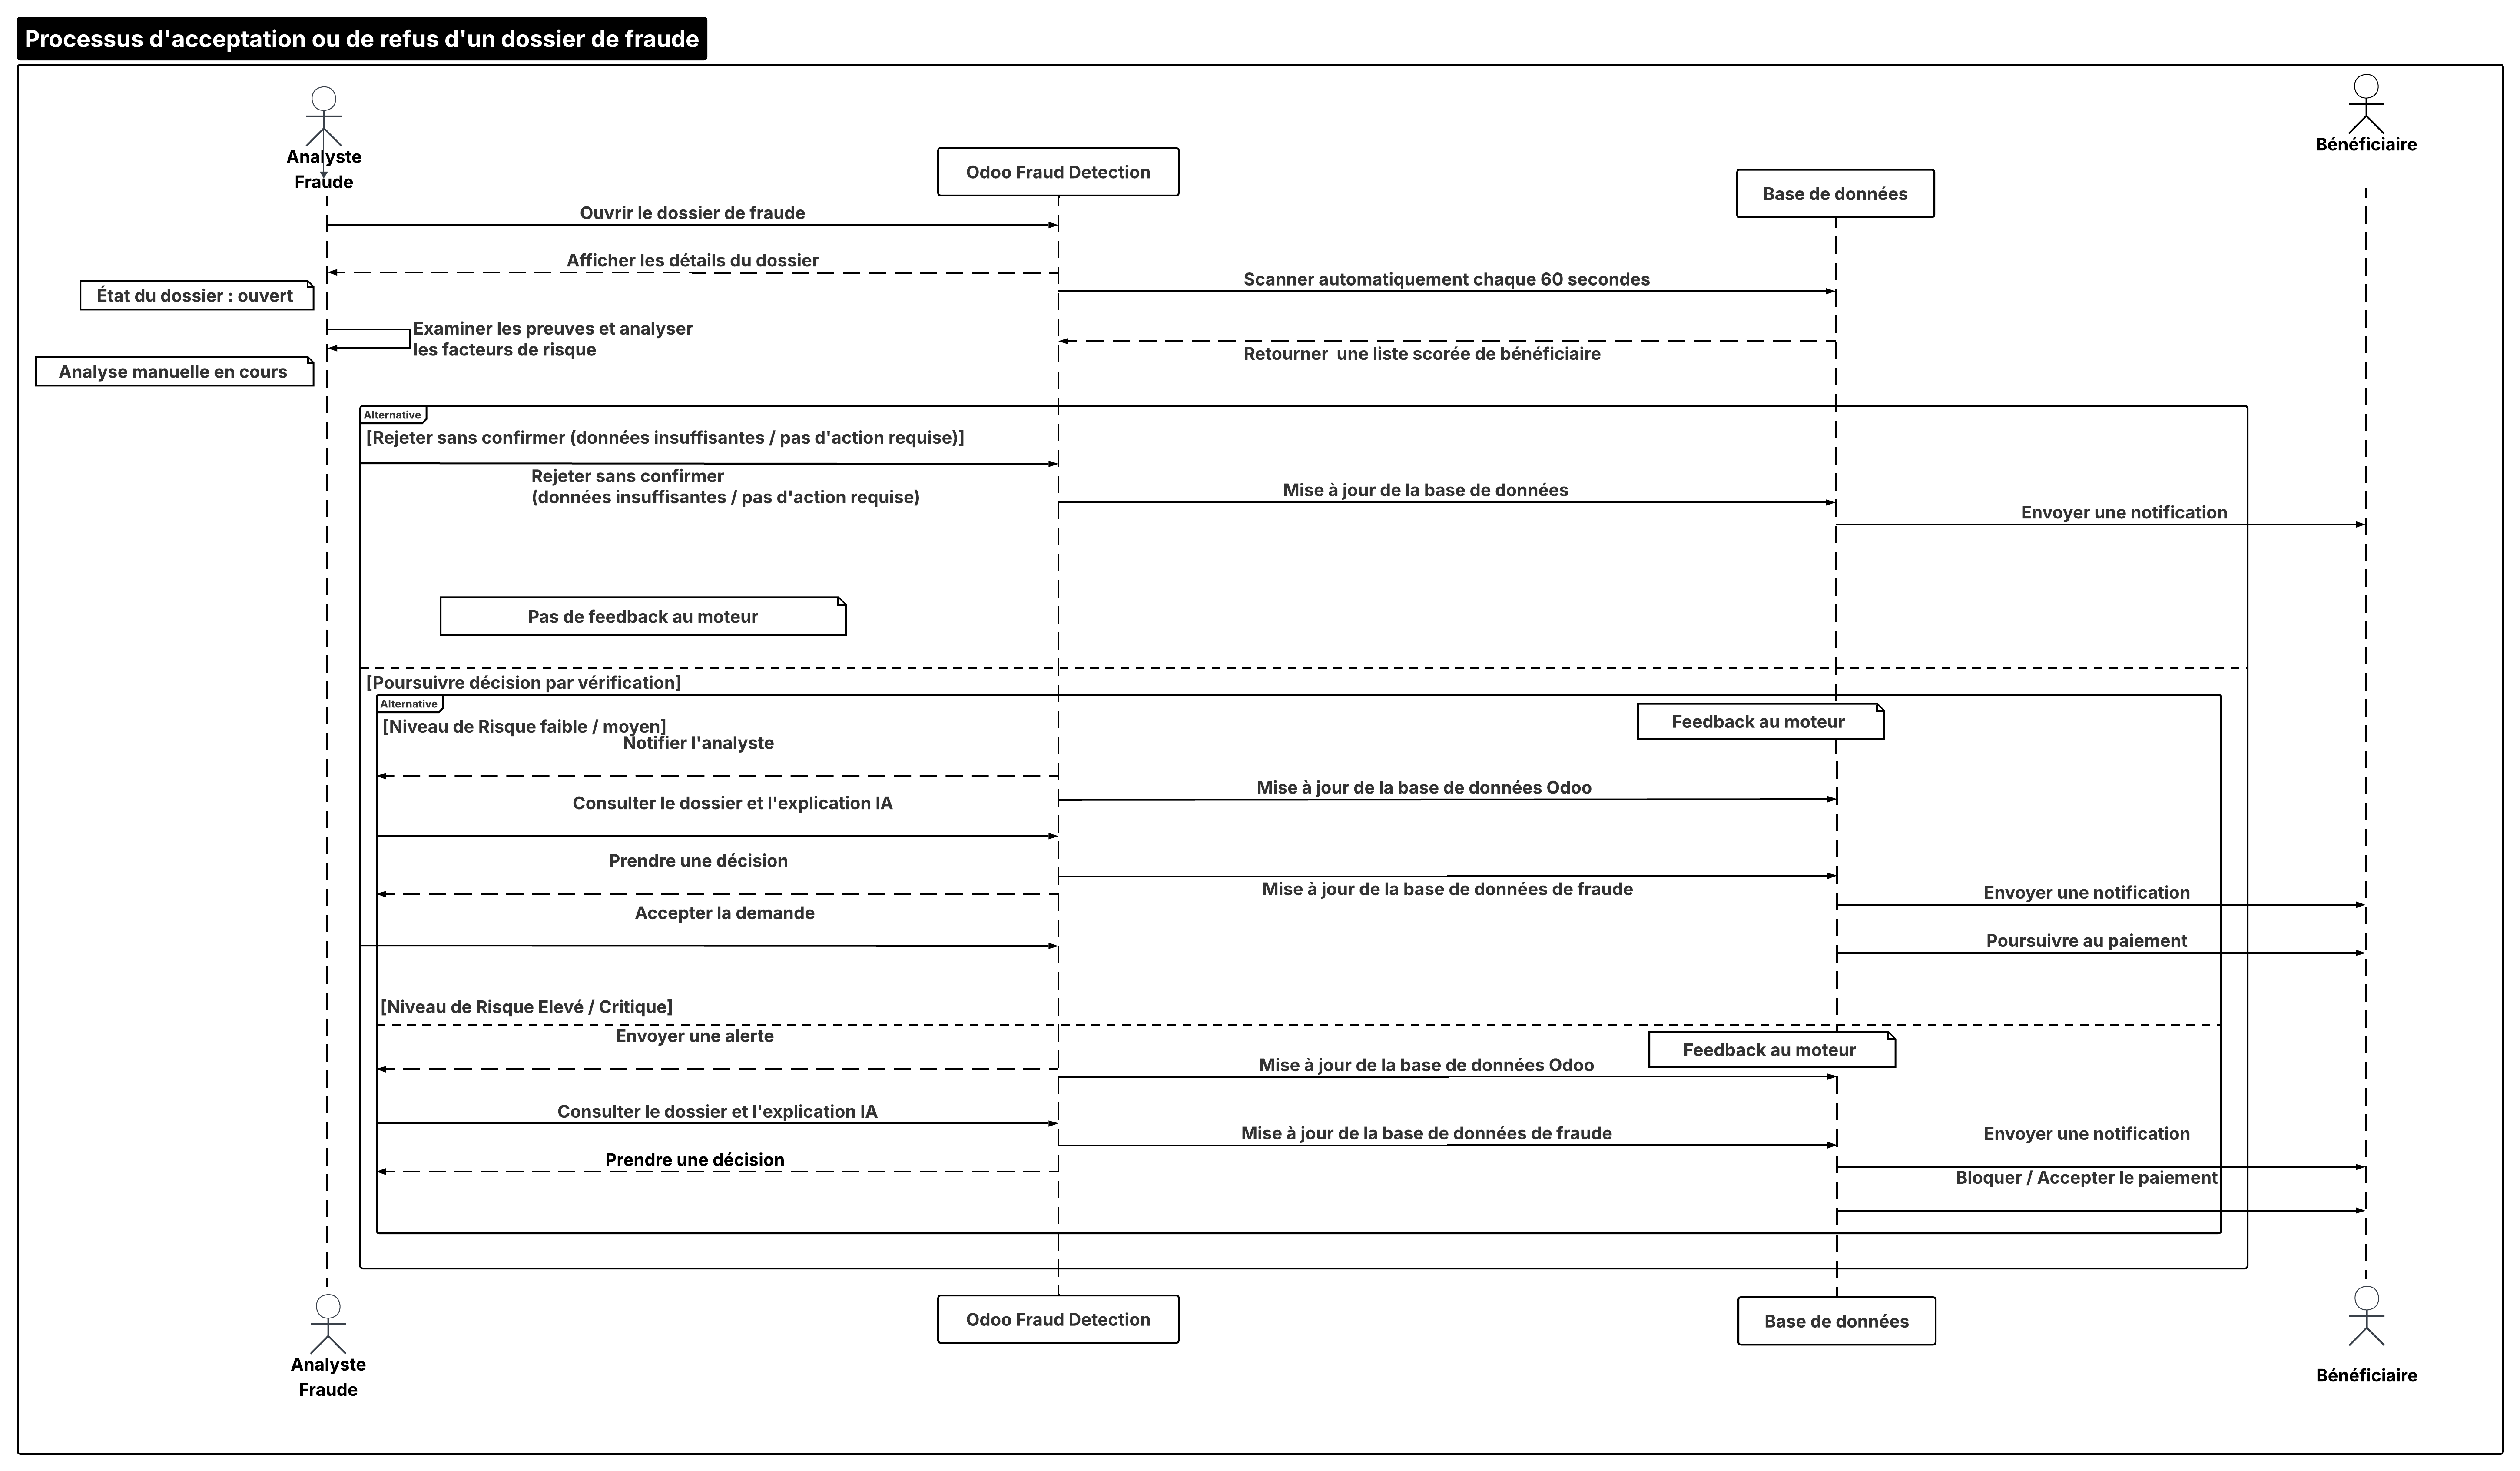
\includegraphics[width=\paperheight,height=0.75\paperwidth,keepaspectratio]{ANALYSTE_FRAUDE_SEQUENCE.png}%
  \caption{Diagramme de séquence : processus d'acceptation ou de refus d'un dossier par l'analyste fraude}
  \label{fig:diagramme-sequence-analyste}
\end{figure}
\end{landscape}

\section{Architectures des composants du moteur de détection de fraude}

\hspace{0.5cm}Afin d'approfondir l'analyse technique, cette section détaille le fonctionnement interne de chaque agent.

\subsection{Pipeline global du moteur de détection (agrégation)}

\begin{figure}[H]
\centering
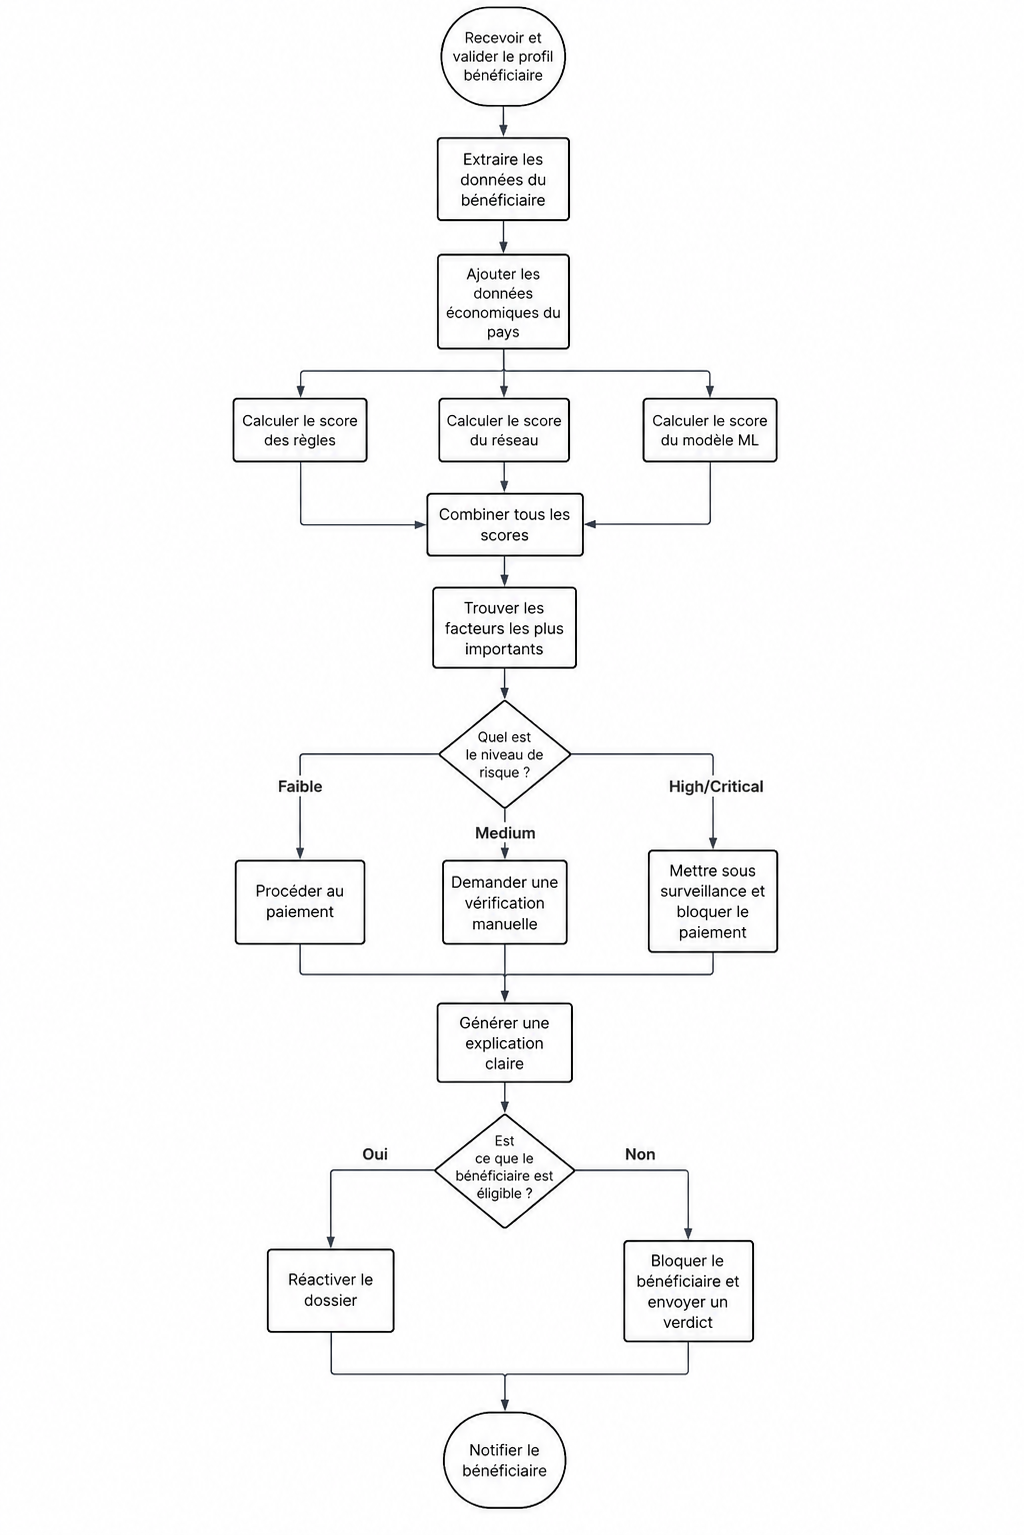
\includegraphics[width=0.75\textwidth]{ProcessGlobal.png}
\caption{Pipeline global d'orchestration du moteur de détection de fraude}
\label{fig:flux-pipeline-global}
\end{figure}

\hspace{0.5cm}Ce pipeline décrit le fonctionnement global du système. Les données du bénéficiaire sont extraites, puis trois scores (règles, réseau et modèle ML) sont calculés en parallèle avant d'être fusionnés en un score de risque unique.


\subsection{Architecture des composants du moteur de détection}

\hspace{0.5cm}Après avoir présenté le fonctionnement global du moteur de détection à travers le pipeline d'orchestration (figure~\ref{fig:flux-pipeline-global}), cette section montre comment ce fonctionnement est organisé dans le code. Le diagramme de classes présente les principaux composants du moteur, leurs responsabilités ainsi que les relations qui les relient. Chaque composant remplit une tâche précise et collabore avec les autres pour produire la décision finale.
\hspace{0.5cm}Le tableau~\ref{tab:composants-ml} résume le rôle des principaux composants représentés dans le diagramme.

\begin{table}[H]
\centering
\footnotesize
\renewcommand{\arraystretch}{1.2}
\begin{tabular}{|p{4.2cm}|p{10.2cm}|}
\hline
\textbf{Composant} & \textbf{Rôle} \\
\hline
DecisionOrchestrator &
Coordonne tout le processus de détection. Il appelle les différents composants, rassemble leurs résultats et produit la décision finale. \\
\hline
FeatureEngineer &
Prépare les données utilisées par le moteur en construisant les caractéristiques (features) du bénéficiaire. \\
\hline
BeneficiaryExtractor &
Récupère les informations du bénéficiaire depuis la base de données OpenG2P. \\
\hline
RuleService &
Calcule le score obtenu à partir des règles métier. \\
\hline
GraphAnalyzer &
Analyse les relations entre bénéficiaires afin d'identifier des connexions ou des comportements suspects. \\
\hline
RelationshipExtractor &
Récupère les liens entre bénéficiaires utilisés par le module d'analyse de réseau. \\
\hline
MultiModelScorer &
Calcule le score de fraude à partir de plusieurs modèles de Machine Learning. \\
\hline
BaseModel &
Interface commune utilisée par les modèles de prédiction. \\
\hline
RandomForestModel, LogisticRegressionModel, XGBoostModel &
Produisent chacun une estimation de la probabilité de fraude. \\
\hline
IsolationForestModel &
Détecte les comportements inhabituels grâce à un modèle de détection d'anomalies. \\
\hline
MetaModel &
Combine les résultats des différents modèles afin d'obtenir un score unique (stacking). \\
\hline
Explainer &
Explique la décision prise et met en évidence les facteurs qui ont le plus influencé le résultat. \\
\hline
FraudCaseRepository &
Enregistre les décisions et conserve l'historique des cas analysés. \\
\hline
\end{tabular}
\caption{Rôle des principaux composants du moteur de détection}
\label{tab:composants-ml}
\end{table}

\hspace{0.5cm}Cette architecture repose sur une séparation claire des responsabilités. Chaque composant réalise une tâche spécifique (extraction des données, règles métier, analyse du réseau, modèles de Machine Learning, explication et stockage des résultats). Cette organisation facilite la maintenance du système ainsi que l'ajout de nouveaux modèles ou de nouvelles règles sans modifier le reste du moteur.
\begin{landscape}
\thispagestyle{plain}

\vspace*{\fill}

\begin{center}

\includegraphics[width=0.92\paperheight]{DiagClassML.png}
\end{center}

\vspace{-0.3cm}

\captionof{figure}{Diagramme de classe des principaux composants du moteur de détection de fraude}
\label{fig:diagramme-classes-ml}

\vspace*{\fill}

\end{landscape}

\subsection{Moteur de règles métier (Rule Engine)}

\hspace{0.5cm}Le moteur de règles constitue la première couche de détection. Il adapte son évaluation au contexte économique grâce au \textit{GNI per capita} fourni par l'API de la Banque Mondiale. Les caractéristiques socio-économiques du bénéficiaire sont ensuite évaluées par dix règles métier pondérées afin de produire un niveau de risque.
\begin{figure}[H]
\centering
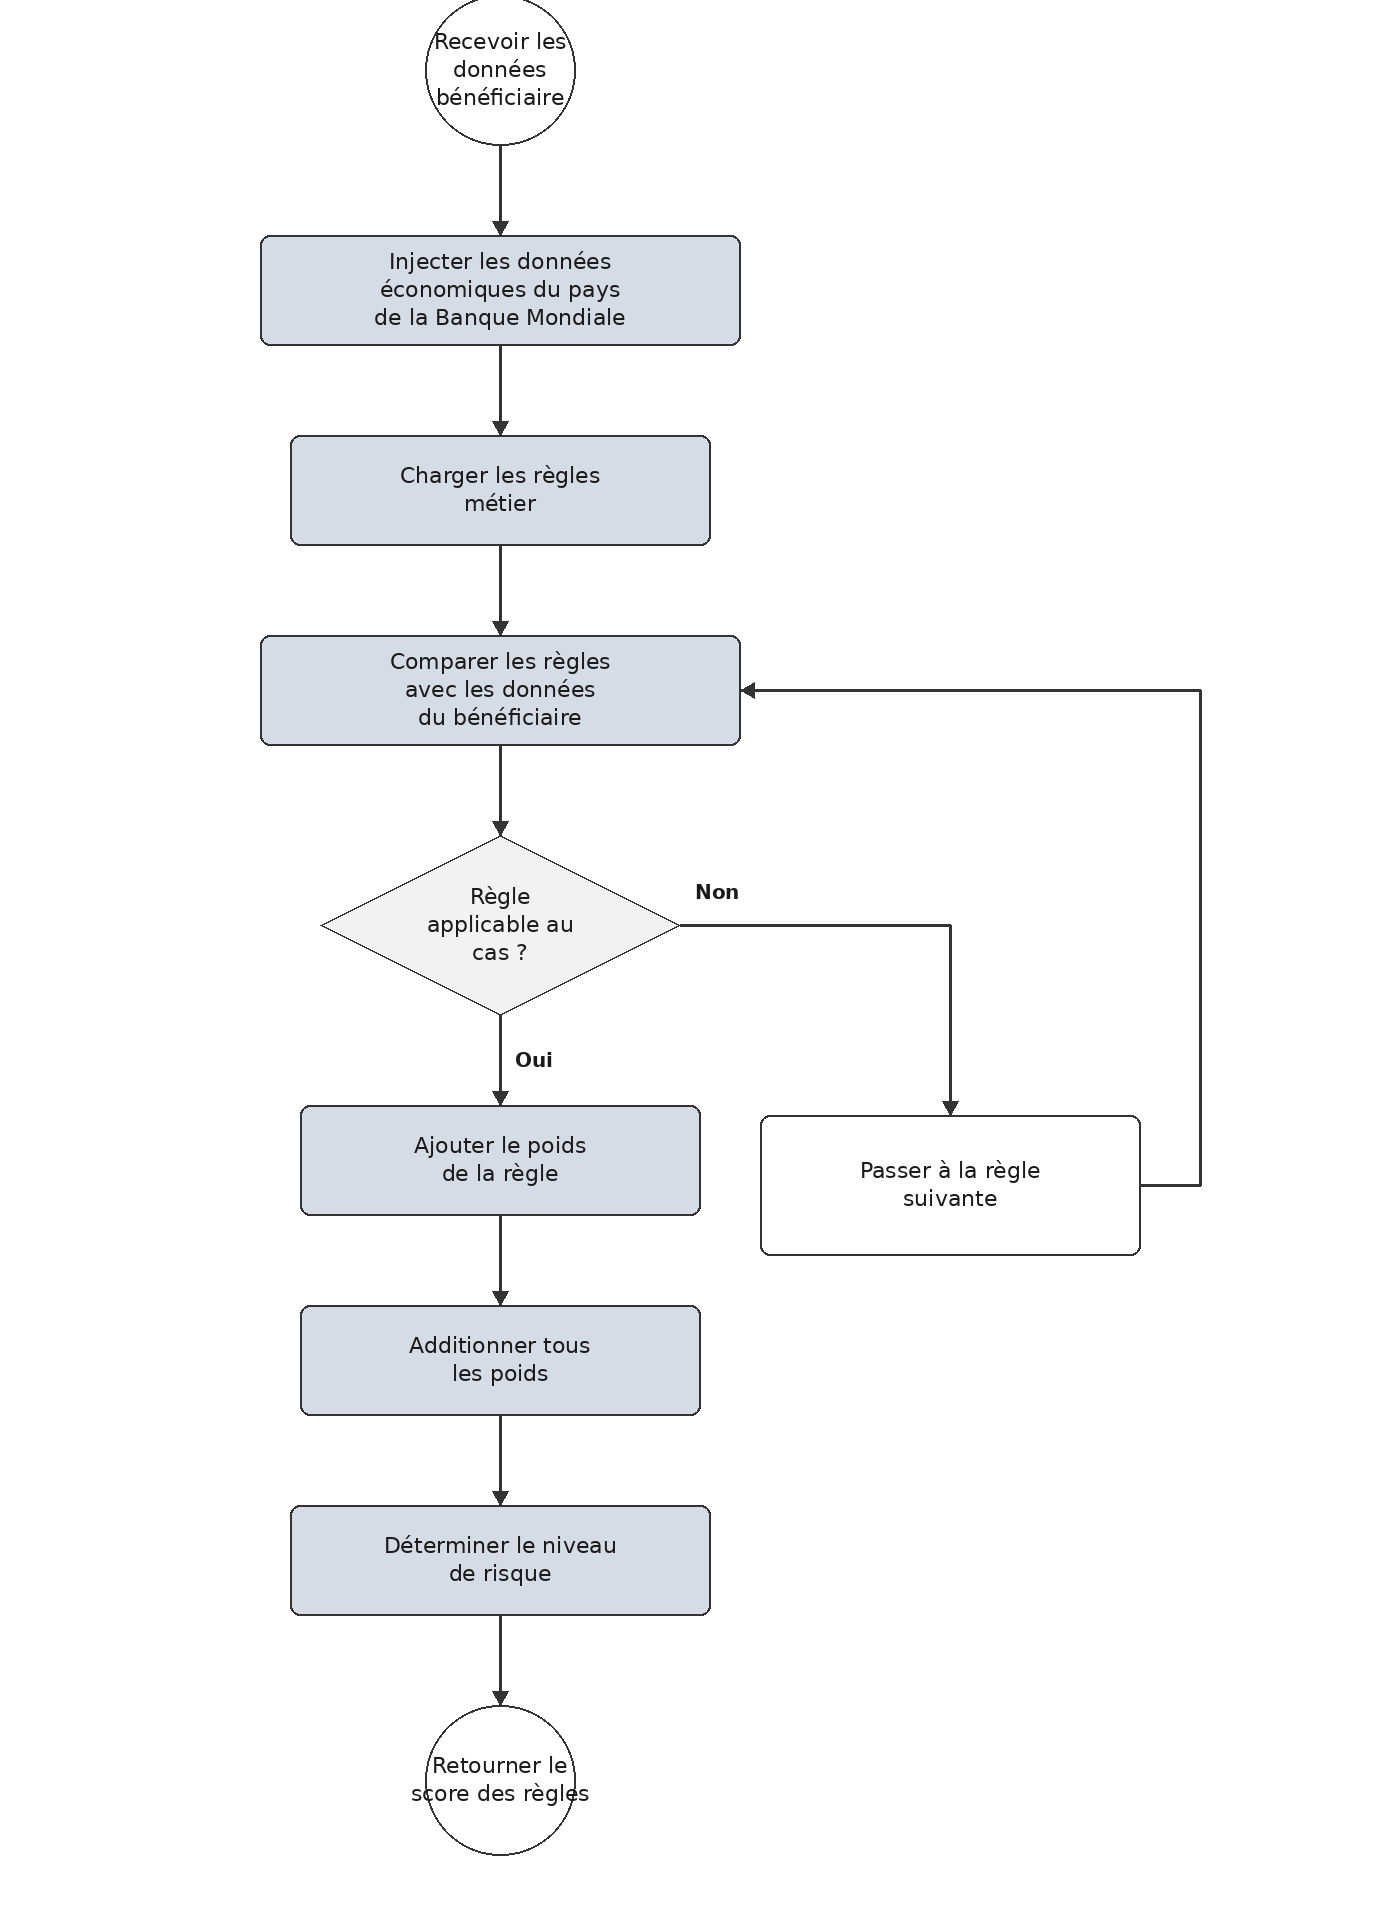
\includegraphics[width=0.68\textwidth]{RuleEngine.png}
\caption{Processus d'évaluation du moteur de règles métier}
\label{fig:flux-rule-engine}
\end{figure}

\begin{table}[H]
\centering
\footnotesize
\renewcommand{\arraystretch}{1.1}
\begin{tabular}{|p{4cm}|p{10.3cm}|}
\hline
\thead{Élément} & \thead{Rôle} \\
\hline
\textbf{API Banque Mondiale} &
Fournit le \textit{GNI per capita} afin d'adapter l'analyse au contexte économique du pays. \\
\hline
\textbf{Seuil de pauvreté} &
Référence utilisée pour détecter les sous-déclarations de revenus. \\
\hline
\textbf{Revenu médian} &
Permet de contextualiser le revenu déclaré selon le pays de résidence. \\
\hline
\textbf{Critères analysés} &
Revenu, taille du ménage, score PMT, nombre de programmes, comptes et téléphones partagés. \\
\hline
\textbf{Score final} &
Somme pondérée des règles satisfaites, convertie en niveau de risque (Low, Medium, High ou Critical). \\
\hline
\end{tabular}
\caption{Éléments clés du moteur de règles}
\label{tab:rule-engine}
\end{table}

\subsection{Analyseur de réseau (Graph)}

\hspace{0.5cm}L'analyseur de réseau examine les liens entre bénéficiaires, notamment le partage de numéros de téléphone ou de comptes bancaires. Il construit un graphe relationnel et calcule l'importance de chaque nœud pour repérer les bénéficiaires fortement connectés à d'autres, un signe potentiel de fraude organisée en réseau.

\begin{figure}[H]
  \centering
  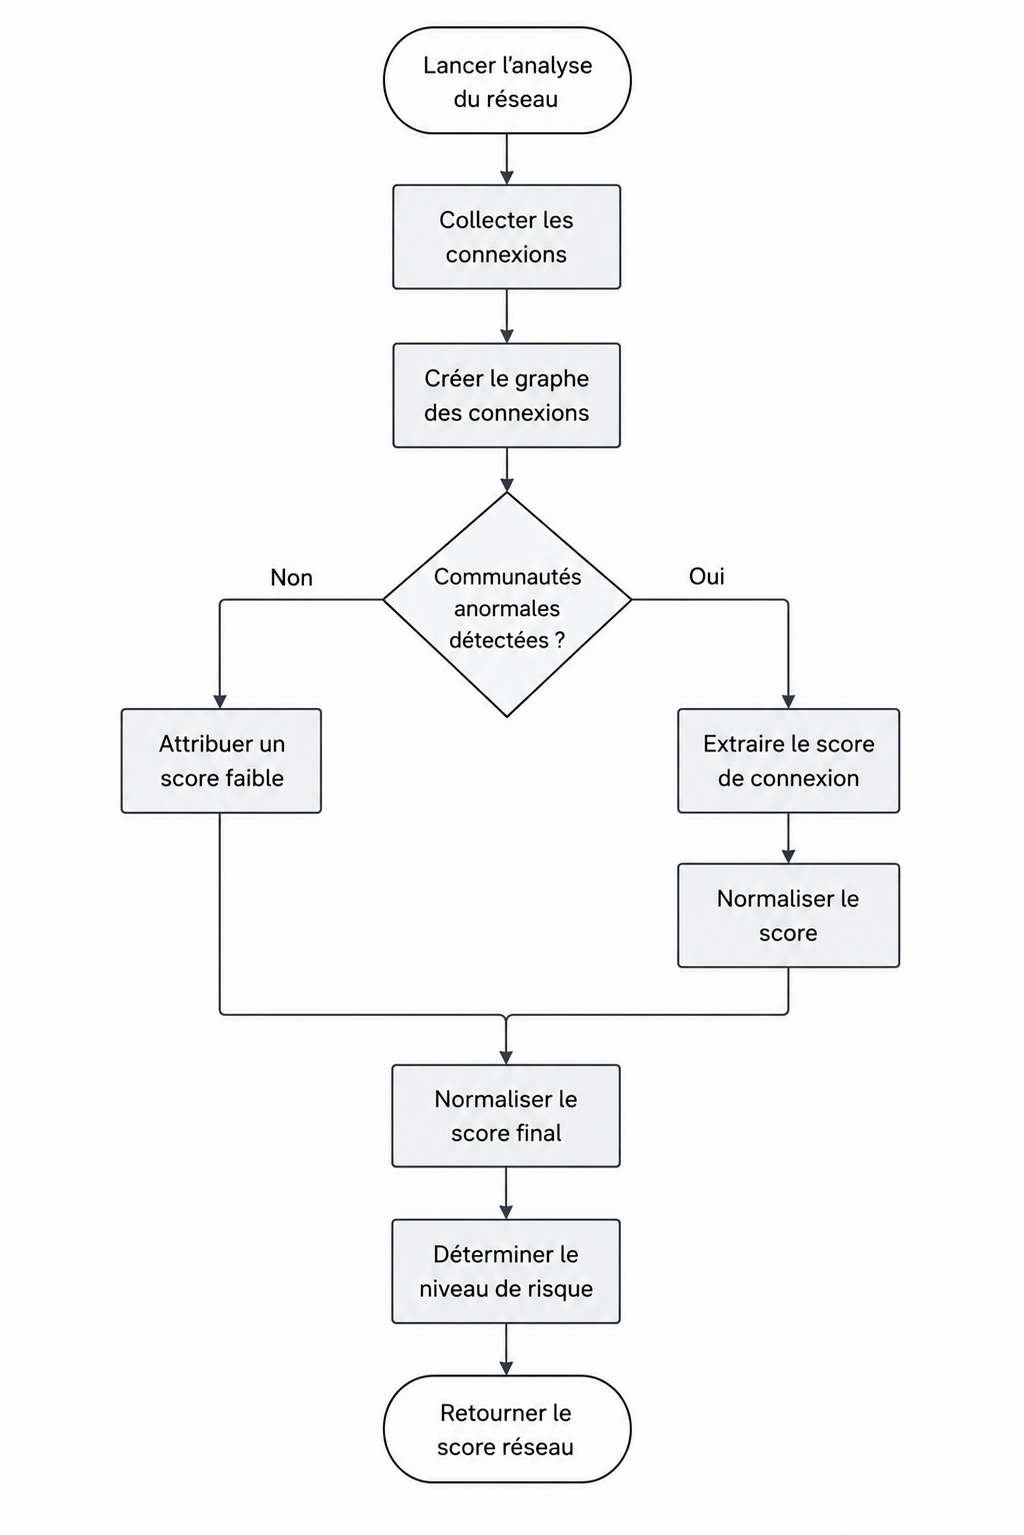
\includegraphics[width=0.60\textwidth]{Graph.png}
  \caption{Processus d'analyse du réseau relationnel des bénéficiaires}
  \label{fig:flux-graph-analyzer}
\end{figure}

\subsection{Explicabilité et génération du texte (SHAP + LLM)}

\hspace{0.5cm}Ce processus se déroule en deux temps. D'abord, le module SHAP analyse la contribution de chaque variable au score et en sélectionne les facteurs les plus déterminants. Ensuite, ces facteurs techniques sont simplifiés et transmis à un modèle de langage (Ollama), qui génère une explication en français compréhensible pour l'analyste.

\begin{figure}[H]
  \centering
  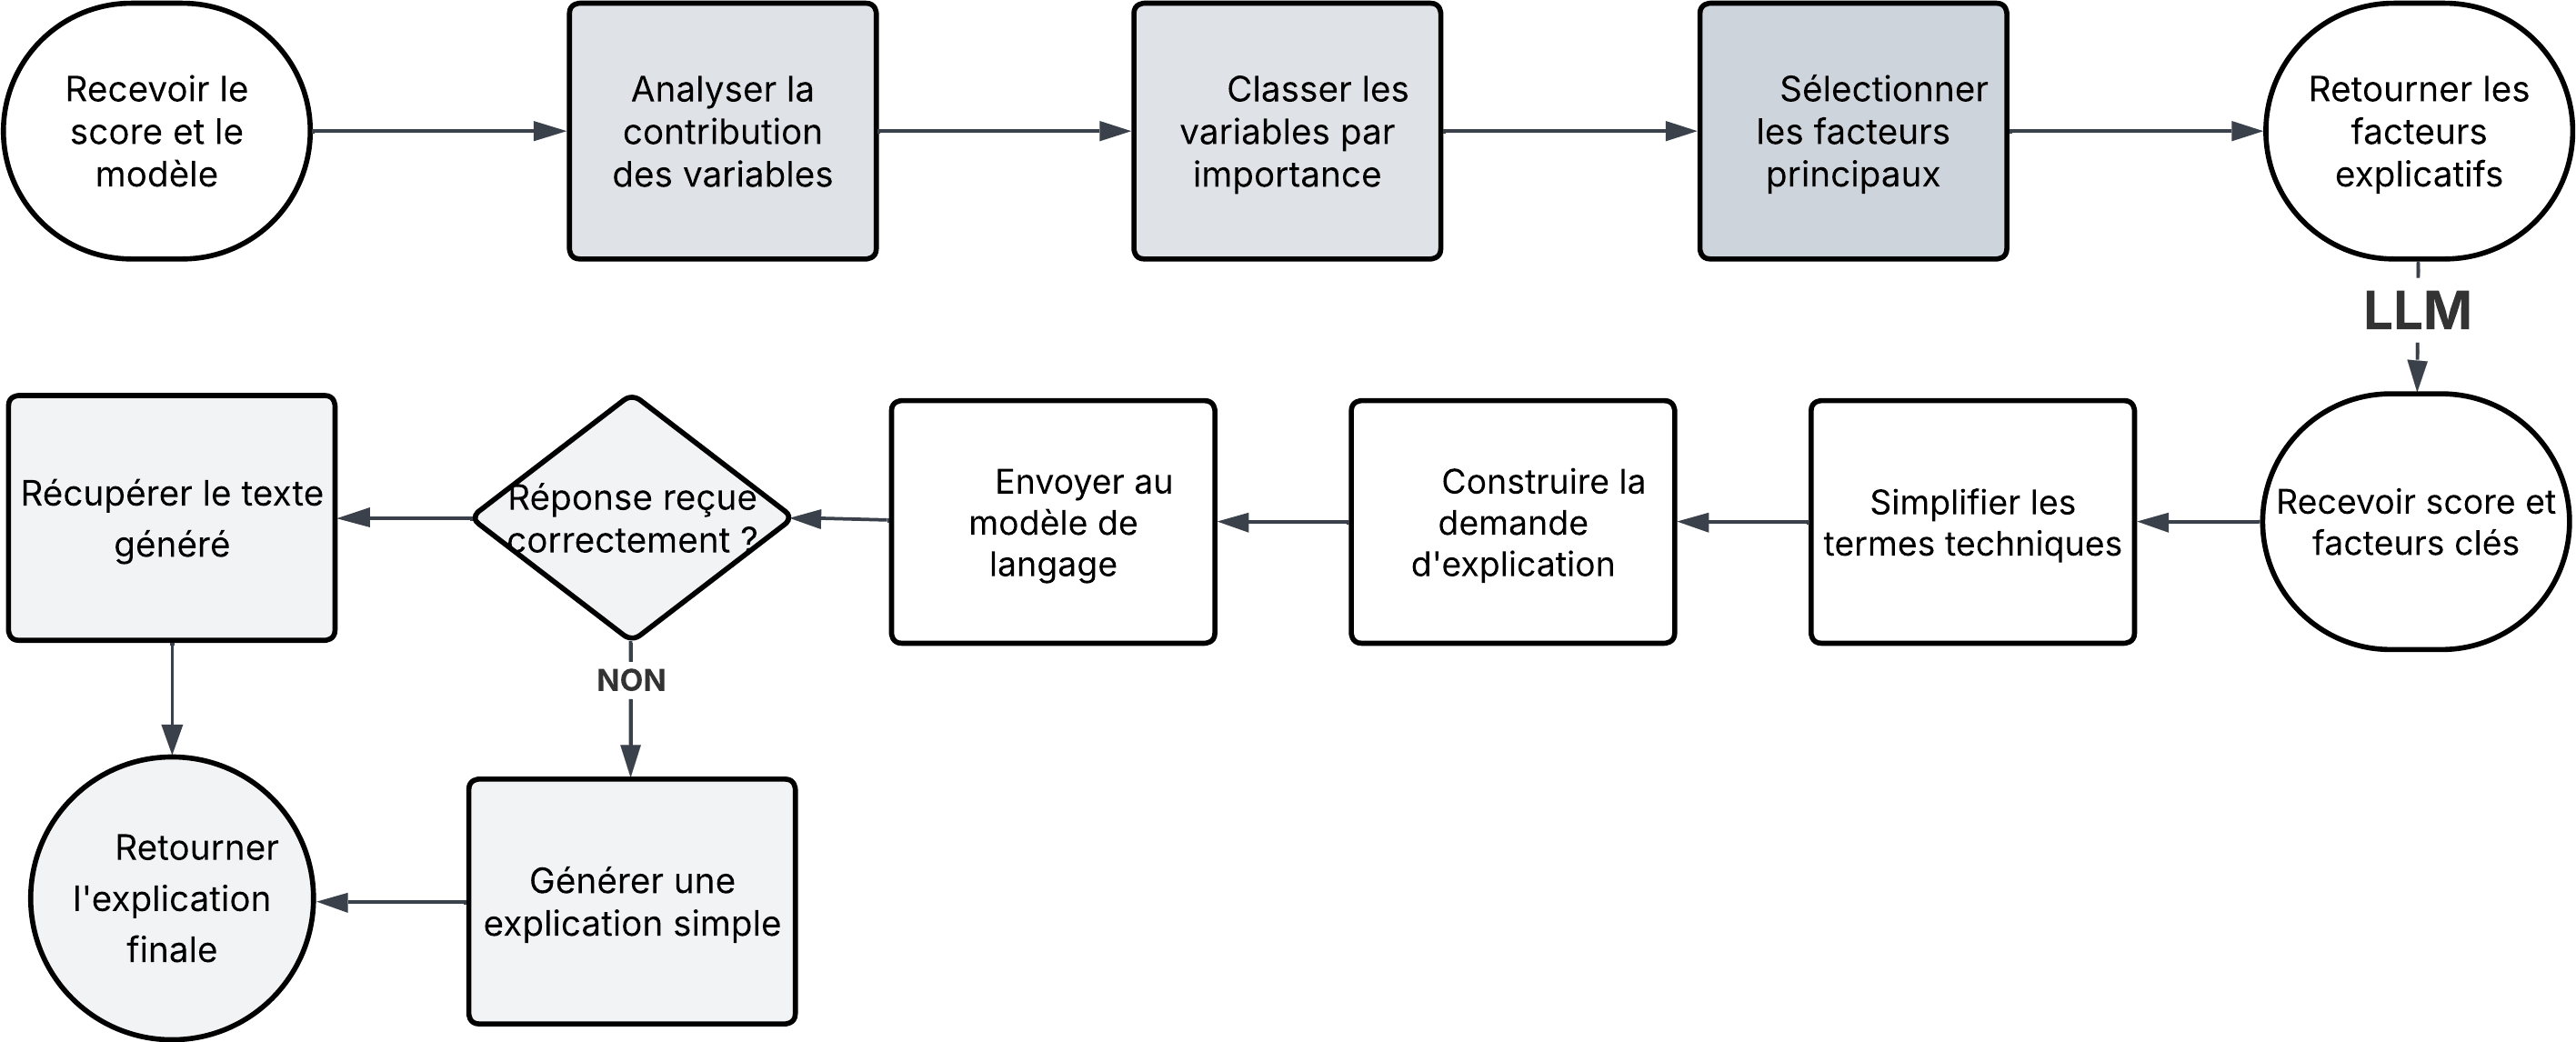
\includegraphics[width=0.95\textwidth]{SHAPLLM.png}
  \caption{Processus d'explicabilité SHAP et de génération d'explication par LLM}
  \label{fig:flux-shap-llm}
\end{figure}


\subsection{Organisation de flux de données}
\hspace{0.5cm} Pour visualiser convenablement l'èchange entre ces classes et ces acteurs, nous présentons le diagramme de flux de données. Ce diagramme illustre comment les données circulent à travers le système, depuis la collecte initiale jusqu'à la génération des alertes et des rapports. Il met en évidence les points d'entrée et de sortie des données, ainsi que les transformations et traitements appliqués à chaque étape du processus.
\begin{figure}[H]
       \centering
          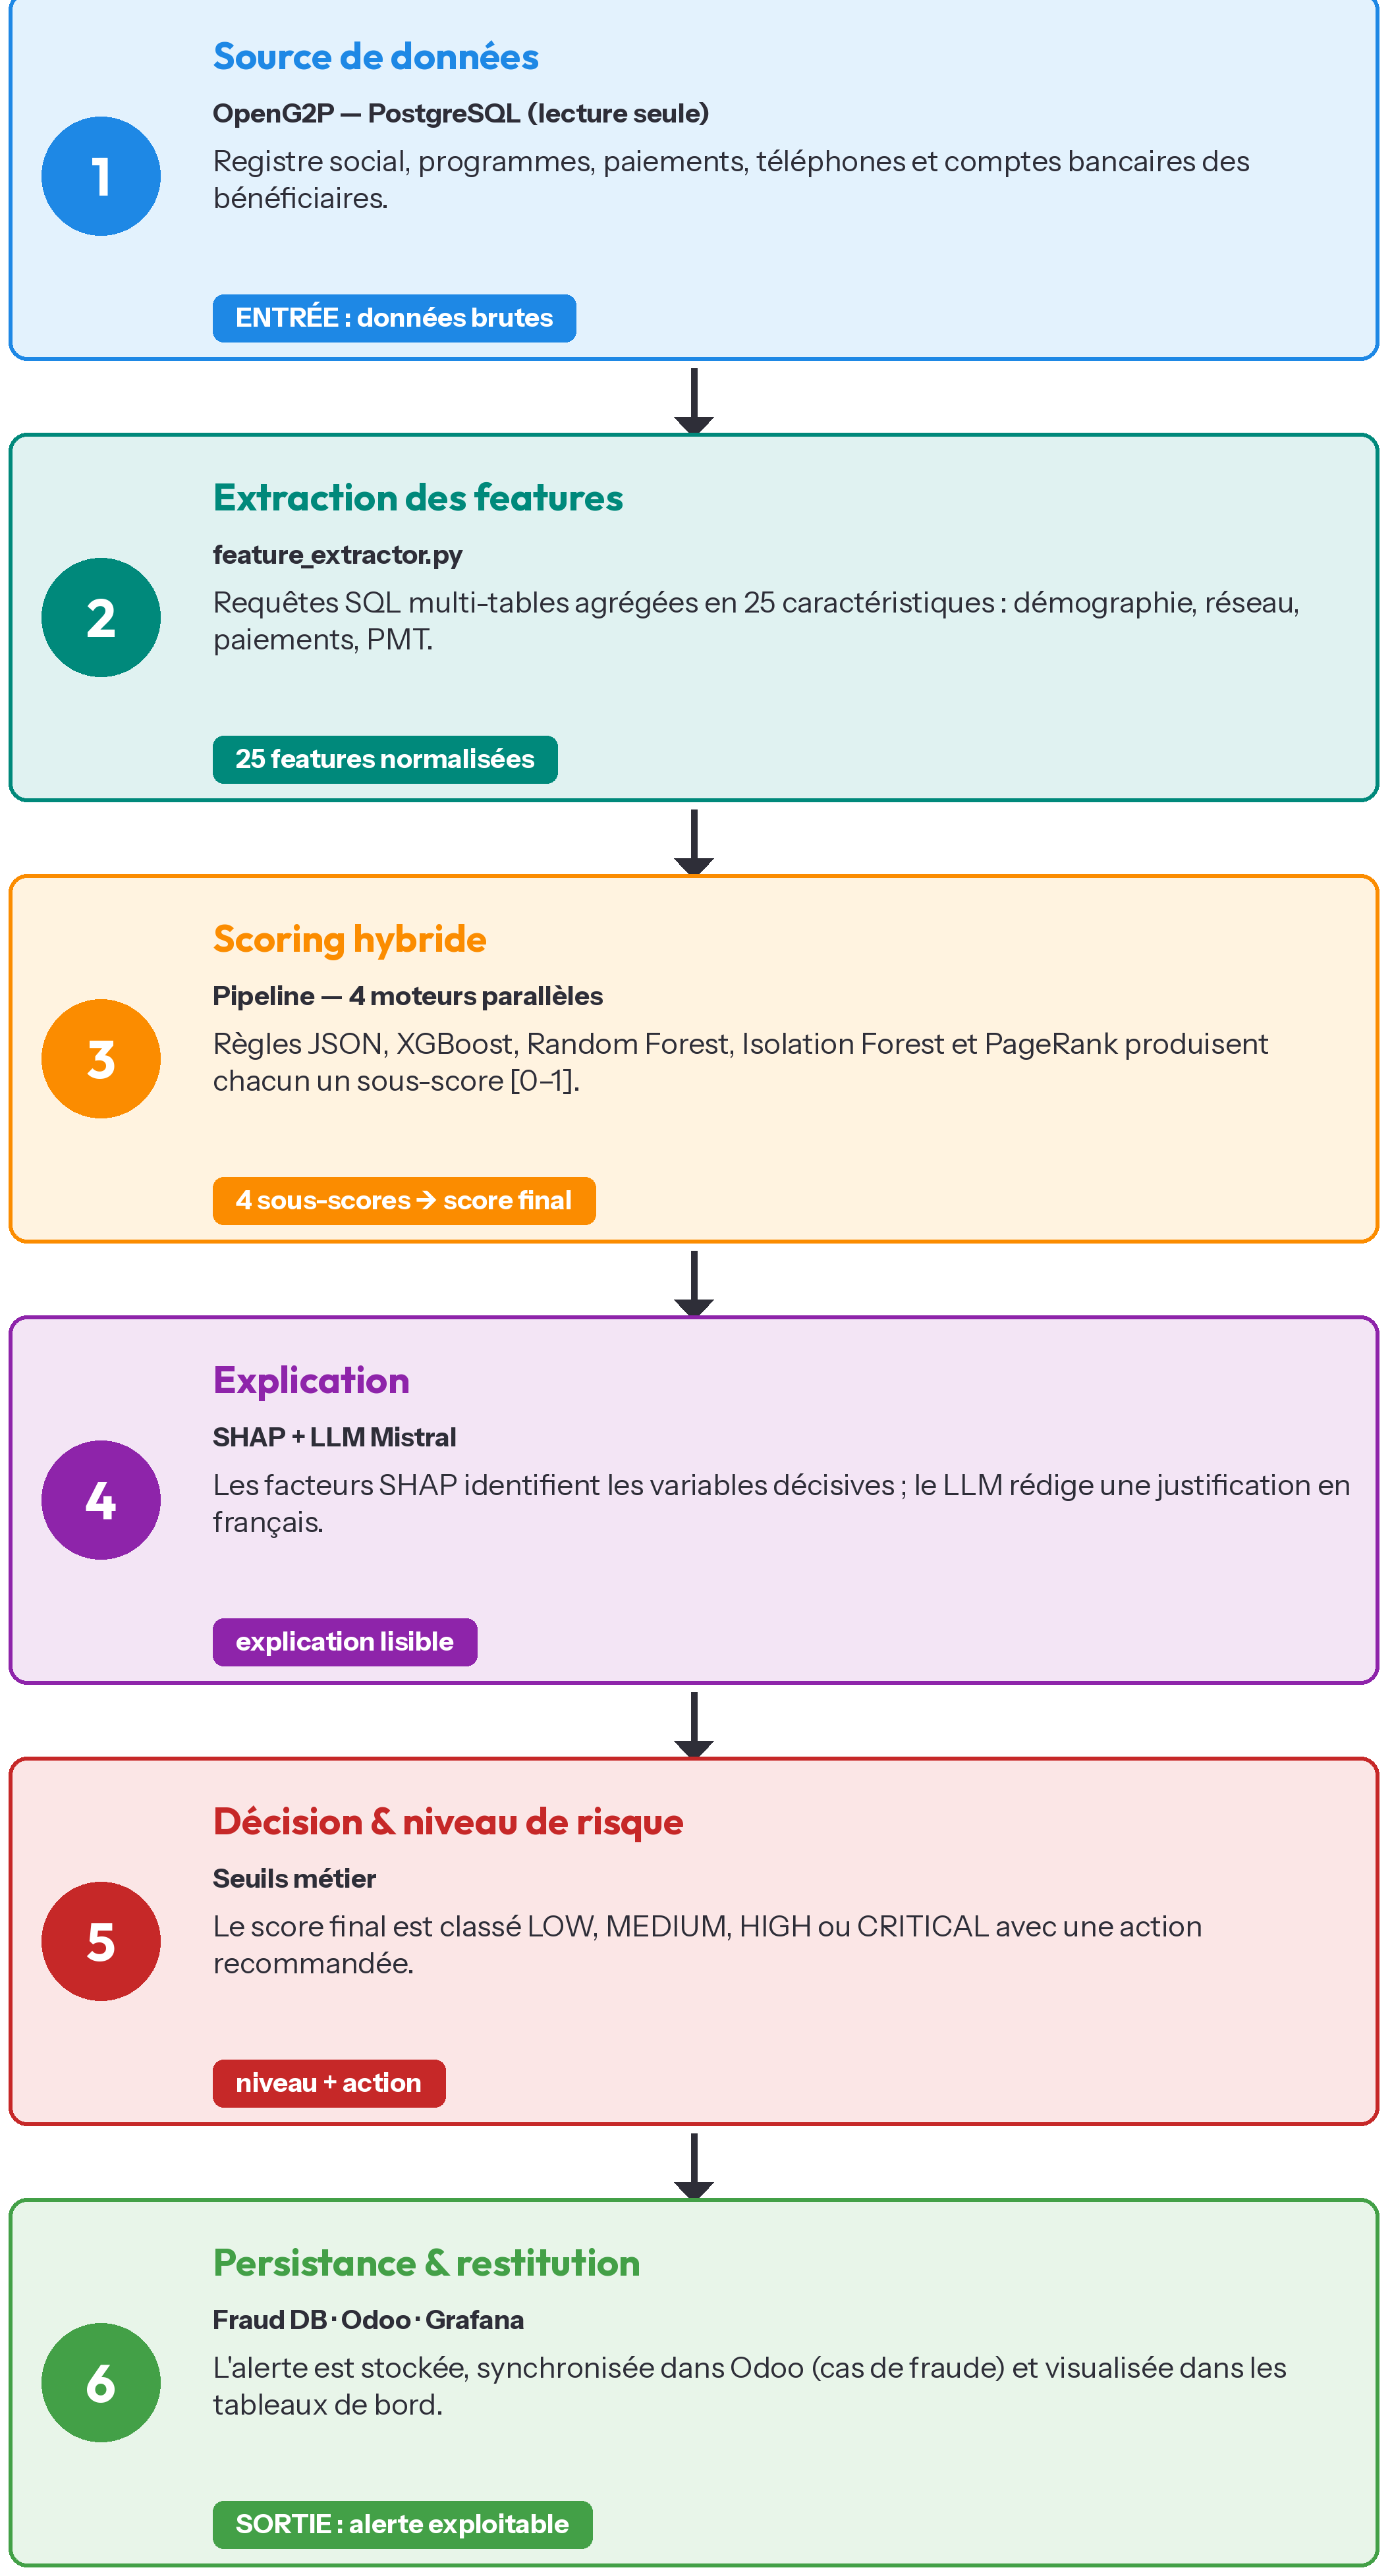
\includegraphics[width=0.72\textwidth,height=0.7\textheight,keepaspectratio]{archi_flux_donnees.png}
     \caption{Diagramme de flux de données du moteur intelligent de détection de fraude}
\end{figure} 

\newpage
\subsection{Architecture physique et logique de la solution}

\hspace{0.5cm}Avant de détailler la mise en œuvre technique du système, il est utile de distinguer deux angles de lecture complémentaires. L'\textbf{architecture physique} répond à la question \og où les composants s'exécutent-ils ? \fg{3.6} : elle décrit les machines, serveurs et services réels qui hébergent l'application, ainsi que les échanges réseau entre eux. L'\textbf{architecture logique}, quant à elle, répond à la question \og comment les données circulent-elles et se transforment-elles ? \fg{} : elle décrit les modules fonctionnels du système et la façon dont ils collaborent, indépendamment de la machine sur laquelle ils tournent. Présenter ces deux vues permet au lecteur de comprendre à la fois \textit{où} notre solution est déployée et \textit{comment} elle traite l'information, depuis les données brutes d'OpenG2P jusqu'au verdict de fraude produit par le moteur d'analyse.
\vspace{0.5cm}
\begin{itemize}[label=\textbullet]

    \item \textbf{Architecture physique:} elle retrace le parcours matériel de la donnée, depuis la base PostgreSQL d'OpenG2P jusqu'au moteur de détection de fraude. Le poste de travail de l'utilisateur \textbf{(agent social ou analyste fraude)} communique avec le serveur d'application Odoo, lequel s'appuie sur le serveur de base de données pour stocker et interroger les informations des bénéficiaires. Ces données sont ensuite acheminées, via le réseau interne orchestré par Docker Compose, vers le serveur FastAPI hébergeant le moteur de fraude, qui sollicite à son tour les services de calcul (modèles ML, base vectorielle ChromaDB, serveur Ollama pour le LLM local). Cette vue matérielle permet d'identifier concrètement les machines impliquées, les protocoles de communication utilisés et les points de latence ou de défaillance potentiels du système.

    \vspace{0.5cm}

    \item \textbf{Architecture logique:} elle décrit le cheminement fonctionnel des données, indépendamment de leur emplacement physique. Les informations brutes des bénéficiaires, extraites d'OpenG2P, sont transformées en un tableau de caractéristiques exploitable. Ce tableau alimente en parallèle quatre modules d'analyse : \textbf{moteur de règles métier}, \textbf{modèle de Machine Learning}, \textbf{détecteur d'anomalies} et \textbf{analyseur de graphe relationnel}  dont les scores sont ensuite agrégés pour produire un score de risque final. Ce score est enrichi par un module d'explicabilité \textbf{(SHAP)} puis traduit en langage naturel par un modèle de langage local, avant d'être restitué à l'analyste fraude sous forme d'alerte exploitable. Cette vue logique met en évidence la logique métier du système et la manière dont chaque composant contribue à la décision finale.

\end{itemize}

\begin{landscape}
\begin{figure}[H]
  \centering
  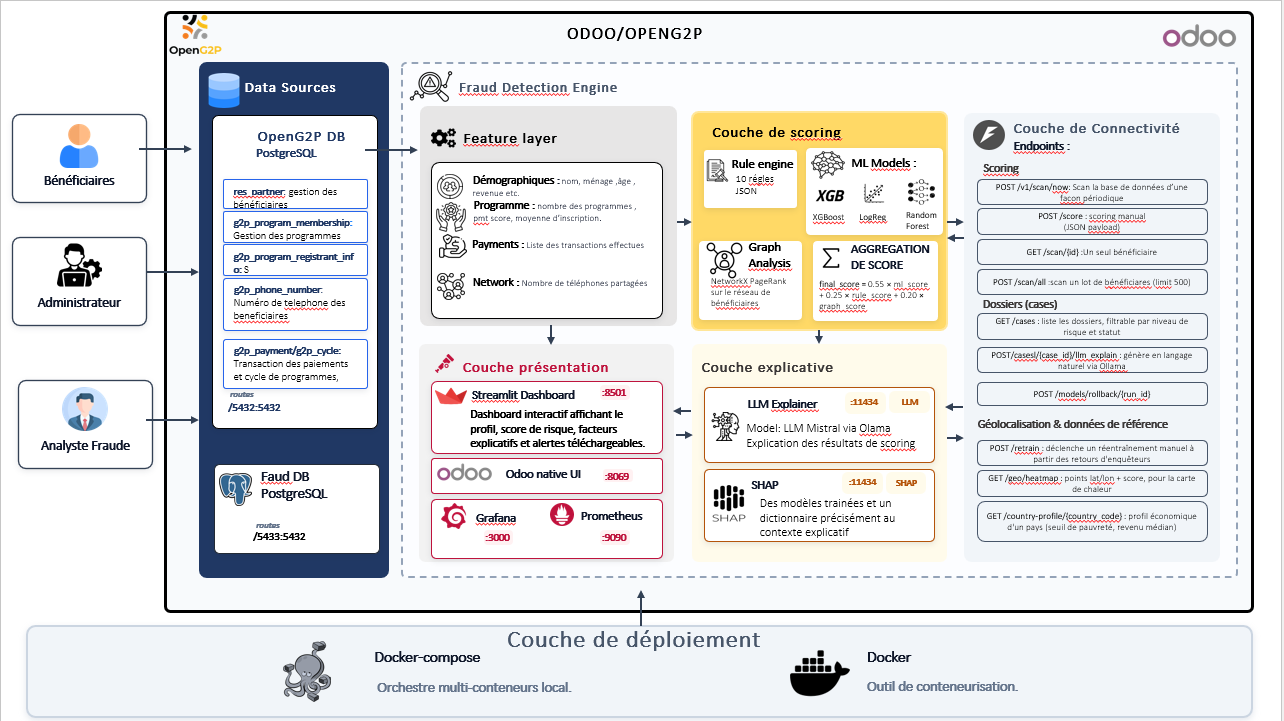
\includegraphics[width=\linewidth,height=\textheight,keepaspectratio]{ArchitectureLogique.png}
  \caption{Architecture logique du moteur intelligent de détection de fraude}
  \label{fig:interaction-composants}
\end{figure}
\end{landscape}

\begin{landscape}
\begin{figure}[H]
     \centering
          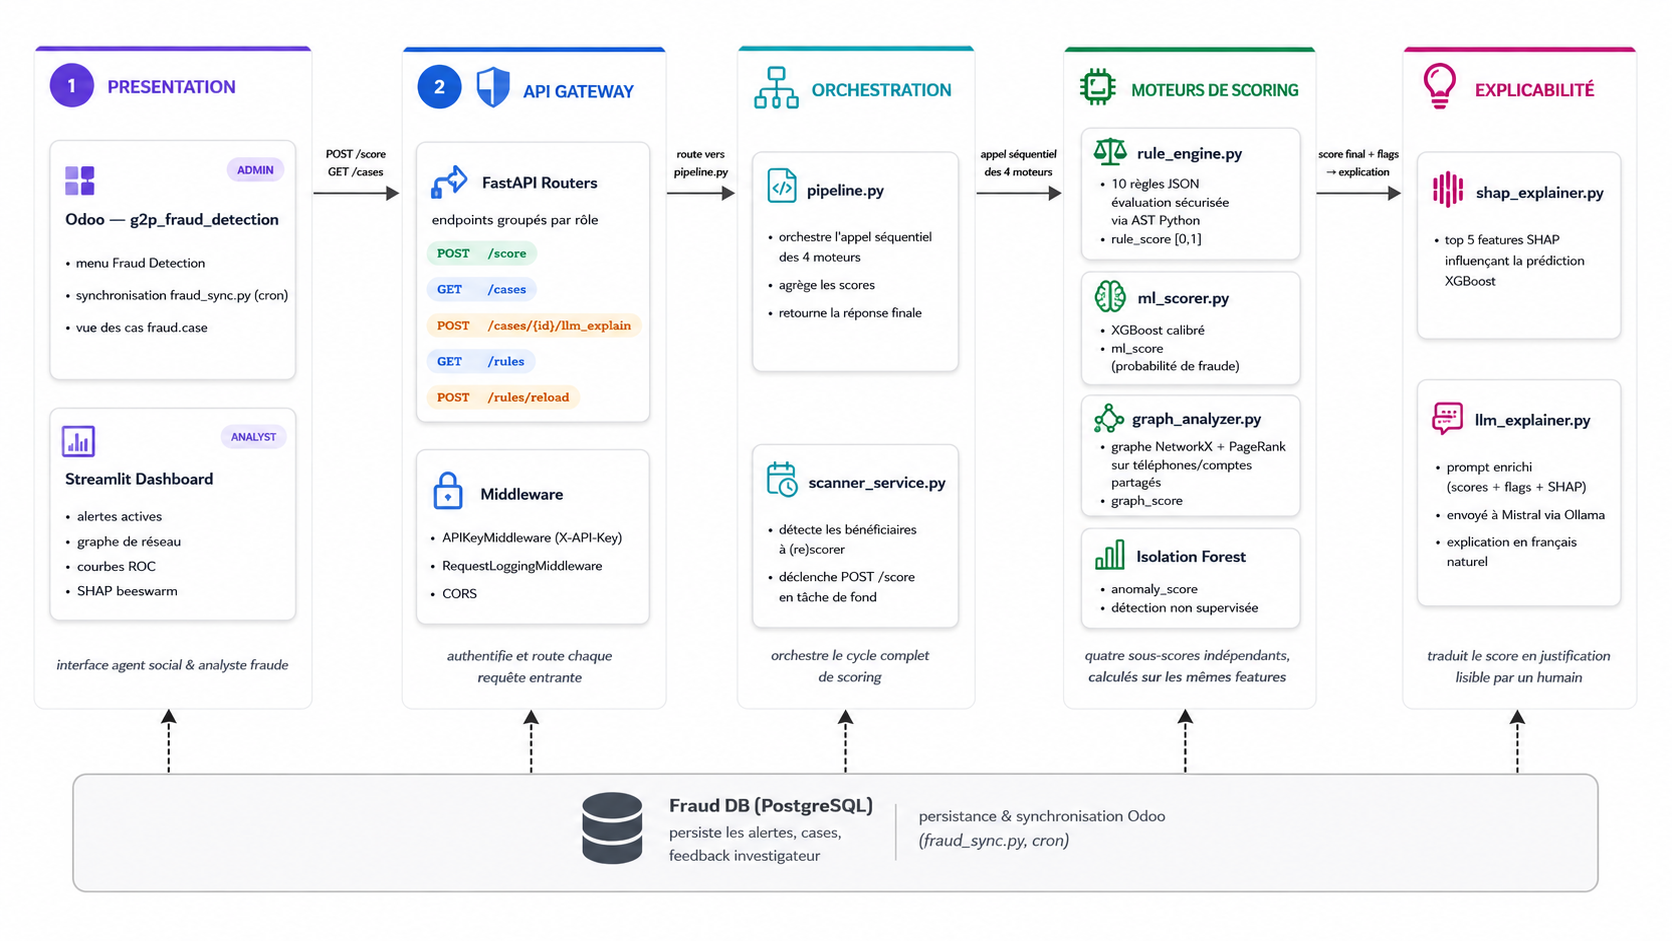
\includegraphics[width=\linewidth,height=\textheight,keepaspectratio]{Modules_principaux.png}
     \caption{Architecture logique du moteur intelligent de détection de fraude}
\end{figure} 
\end{landscape}

\hspace{0.5cm}Notre solution s'appuie sur une architecture hybride et modulaire, combinant des composants d'intelligence artificielle (apprentissage automatique, graphes, explicabilité), des règles métier paramétrables, et une infrastructure cloud-native. Cette approche multicouche nous permet de couvrir un maximum de scénarios de fraude tout en restant auditables et transparentes vis-à-vis des parties prenantes.

\hspace{0.5cm}Après avoir présenté les différents composants du moteur de détection de fraude et leur rôle dans le processus de décision, il est nécessaire de s'intéresser aux technologies ayant permis leur développement. Chaque composant s'appuie sur des outils spécialisés pour assurer le traitement des données, l'apprentissage automatique, l'analyse des relations, l'explicabilité des résultats ainsi que le déploiement de la solution.

\subsection{Stack Technologique}

\hspace{0.5cm}La Figure~\ref{fig:tech-stack} illustre l'environnement technologique adopté, en regroupant les principaux langages, bibliothèques, frameworks et outils utilisés tout au long du projet.
\begin{figure}[H]
    \centering
    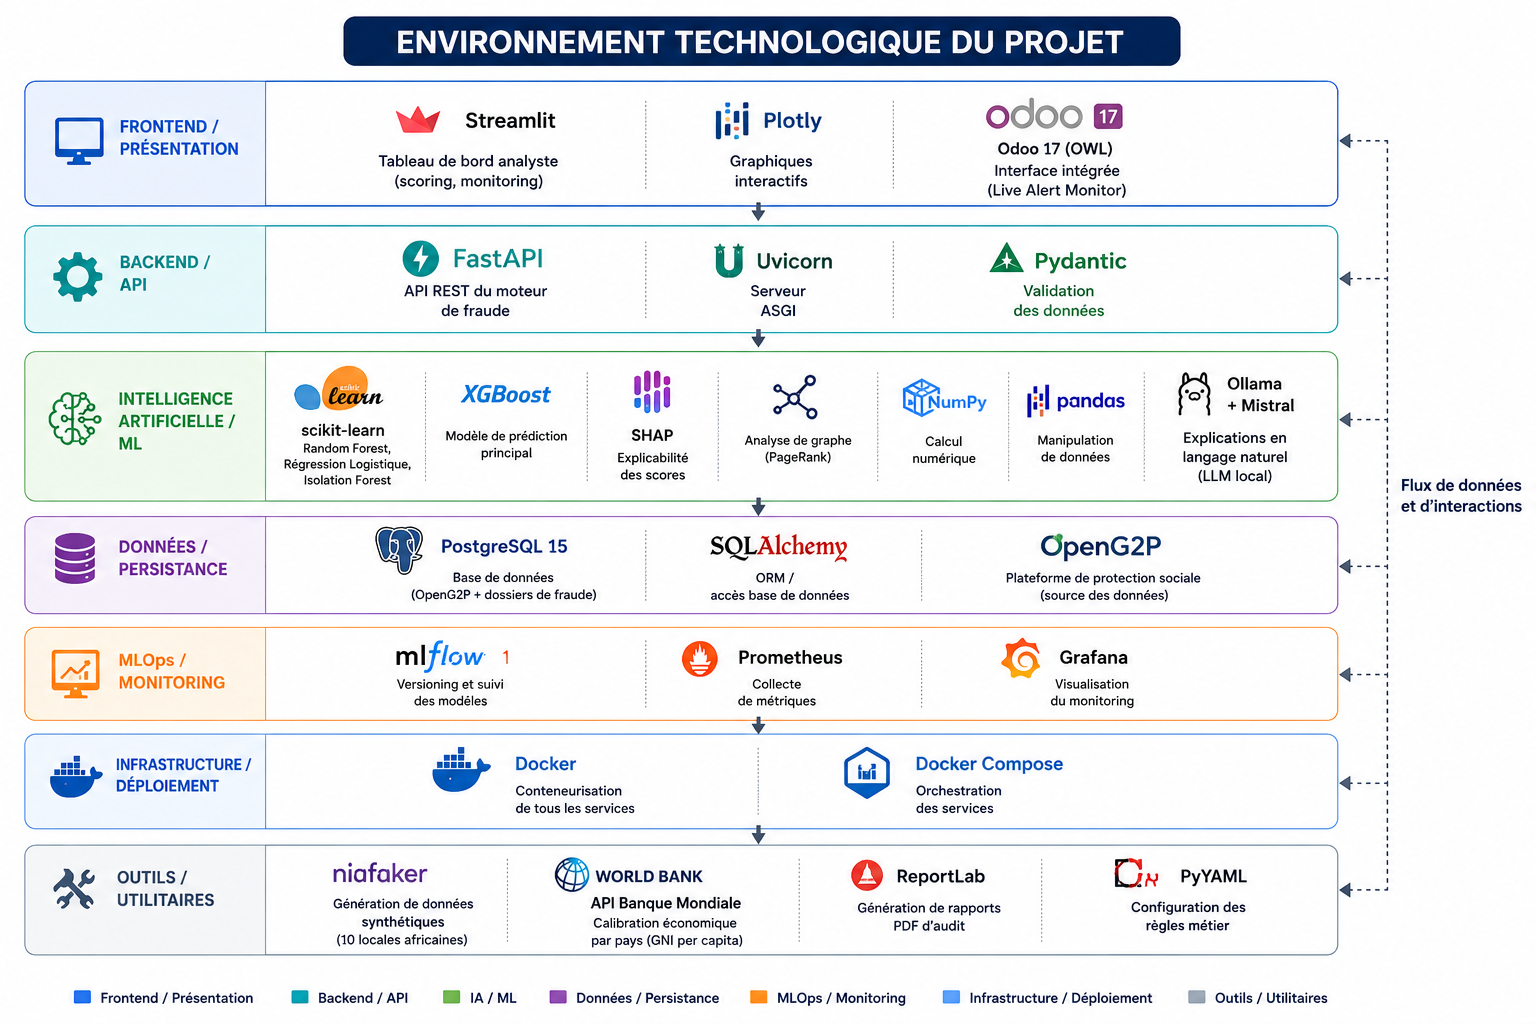
\includegraphics[width=0.92\textwidth, height=0.52\textheight]{TechStack.png}
    \caption{Langages et outils utilisés pour le développement du moteur intelligent de détection de fraude}
    \label{fig:tech-stack}
\end{figure}

\title{Stack de développement backend et données}
\begin{table}[H]
\centering
\renewcommand{\arraystretch}{1.5}
\begin{tabular}{|p{3.5cm}|p{11.8cm}|}
\hline
\thead{Composant} & \thead{Technologie / Description} \\
\hline
\textbf{Base de données} & \textbf{PostgreSQL:} Système de gestion de base de données relationnelle open source hautement fiable, avec support complet du SQL et des transactions ACID. Utilisé pour persister les données d'enregistrement des bénéficiaires, les alertes de fraude et l'historique des décisions. \\
\hline
\textbf{Système intégré} & \textbf{OpenG2P / Odoo 17:} Plateforme open-source de gestion de programmes de protection sociale. Manage l'enregistrement des bénéficiaires, l'administration des programmes d'aide et l'intégration de notre moteur de détection de fraude. \\
\hline
\textbf{ML et graphe} & \textbf{Python (scikit-learn, XGBoost, NetworkX, IsolationForest, RandomForest, Linear Regression):} Écosystème utilisé pour développer les modèles de machine learning, l'extraction de caractéristiques et l'analyse de graphe. \\
\hline
\end{tabular} 
 
\caption{Technologies de base du système de détection de fraude}
\end{table}
\begin{table}[H]
\centering
\renewcommand{\arraystretch}{1.5}
\begin{tabular}{|p{3.5cm}|p{11.8cm}|}
\hline
\thead{Couche} & \thead{Outil / Technologie} \\
\hline
\textbf{Explicabilité} & \textbf{SHAP:} Bibliothèque Python pour l'interprétabilité calculant la contribution de chaque caractéristique au score de fraude. \textbf{Mistral via Ollama:} Modèle de langue généraliste exécuté localement pour transformer les coefficients SHAP et règles en explications textuelles en français. \\
\hline
\textbf{Analyse de graphe} & \textbf{Neo4j:} Base de données graphe pour stocker et analyser les réseaux de bénéficiaires (partage de téléphones, comptes bancaires). Permet la détection de communautés frauduleuses et le calcul de centralité (PageRank). \\
\hline
\textbf{Gestion des modèles} & \textbf{MLflow:} Plateforme pour la gestion du cycle de vie des modèles ML. Enregistre les hyperparamètres, métriques de performance (AUC, précision, rappel) et permet un rollback facilité. \\
\hline
\end{tabular}
\caption{Technologies d'explicabilité et de gestion des modèles}
\end{table}

\newpage
\subsubsection{Stack de développement et DevOps}

\hspace{0.5cm}Pour assurer la qualité, la maintenabilité et le déploiement continu de notre solution, nous avons intégré des outils modernes de développement et d'automatisation :

\begin{table}[H]
\centering
\renewcommand{\arraystretch}{1.5}
\begin{tabular}{|p{3.5cm}|p{11.8cm}|}
\hline
\thead{Catégorie} & \thead{Outil / Framework} \\
\hline
\textbf{Éditeur de code} & \textbf{Visual Studio Code:} Éditeur léger offrant le débogage intégré, autocomplétion intelligente, intégration native de Git et extensions pour Python, SQL et Docker. \\
\hline
\textbf{Gestion de version} & \textbf{Git / GitHub:} Système de contrôle de version pour la collaboration, suivi des changements et gestion des branches. GitHub héberge le dépôt avec workflows d'intégration continue. \\
\hline
\textbf{Containerisation} & \textbf{Docker:} Plateforme de containerisation pour packager l'application avec toutes ses dépendances. Assure la cohérence entre développement, test et production. \\
\hline
\textbf{Orchestration} & \textbf{Docker Compose:} Outil d'orchestration de conteneurs permettant de définir et de lancer l'ensemble de l'infrastructure applicative (backend, base de données, services auxiliaires) via un fichier de configuration YAML unique. Facilite les déploiements reproductibles et le développement local multi-conteneur. \\
\hline
\end{tabular}
\caption{Outils de développement et d'infrastructure}
\end{table}


\subsubsection{Dashboards et visualisation des résultats}
\hspace{0.5cm}Au-delà de la détection elle-même, il est essentiel de fournir aux différents utilisateurs (analystes fraude, superviseurs, administrateurs) des interfaces de visualisation intuitive et interactive. Notre solution intègre plusieurs couches de dashboards et de reporting :

\begin{table}[H]
\centering
\renewcommand{\arraystretch}{1.5}
\begin{tabular}{|p{3.5cm}|p{11.8cm}|}
\hline
\thead{Dashboard / Plateforme} & \thead{Description et cas d'usage} \\
\hline
\textbf{Streamlit - Interface analytique} & Plateforme web interactive développée en Python permettant aux analystes fraude et superviseurs de consulter les alertes détectées, visualiser les explications SHAP en temps réel, et accéder à des statistiques globales de fraude. Le dashboard Streamlit offre une réactivité immédiate et permet des filtres dynamiques (par zone géographique, programme, niveau de risque). \\
\hline
\textbf{MLflow - Suivi des modèles} & Tableau de bord dédié au versionnage et au monitoring des modèles ML. Permet de comparer les performances de différentes versions du modèle (AUC, précision, rappel), de visualiser les métriques d'entraînement, et de tracer la provenance de chaque artefact ML. Essential pour la gouvernance et la reproductibilité. \\
\hline
\textbf{Heatmap géographique} & Visualisation cartographique interactive montrant la concentration géographique des alertes de fraude détectées. Chaque zone est colorée proportionnellement au nombre et à la sévérité des cas signalés, permettant aux superviseurs d'identifier rapidement les hotspots de fraude et d'adapter les stratégies d'investigation par région. \\
\hline
\textbf{Tableau de bord superviseur} & Vue synthétique affichant les KPI globaux : nombre total de cas analysés, taux de fraude détecté, proportion de vrais positifs, tendances temporelles, distribution par niveau de risque, et état des investigations en cours. Utilisé par les décideurs pour le monitoring stratégique du programme. \\
\hline
\textbf{Système de reporting automatisé} & Génération automatique de rapports PDF ou CSV consolidant les résultats de détection, les explications SHAP, les analyses de réseau et les recommandations d'action pour chaque bénéficiaire signalé. Ces rapports sont exportables pour audit externe ou communication auprès du management. \\
\hline
\end{tabular}
\caption{Dashboards et plateformes de visualisation}
\end{table}

\hspace{0.5cm}Ces outils de visualisation sont complémentaires aux couches techniques : tandis que MLflow assure la traçabilité des modèles côté développement, Streamlit et les dashboards superviseur fournissent des interfaces métier accessibles aux non-techniciens. La heatmap géographique facilite le diagnostic spatial de la fraude, et le système de reporting garantit que chaque décision prise peut être justifiée et auditée.

\subsubsection{Collaboration et documentation}

\hspace{0.5cm}Enfin, pour faciliter la communication entre les membres de l'équipe et maintenir une documentation à jour :

\begin{table}[H]
\centering
\begin{tabular}{|p{3.5cm}|p{11.8cm}|}
\hline
\thead{Fonction} & \thead{Outil} \\
\hline
\textbf{Tests et validation d'API} & \textbf{Postman / Swagger:} Clients HTTP interactifs pour tester manuellement et automatiquement l'API REST du moteur de fraude. Permettent de vérifier les endpoints, les paramètres, les codes de retour et de générer de la documentation API automatique. \\
\hline
\textbf{Monitoring opérationnel} & \textbf{ELK Stack (Elasticsearch, Logstash, Kibana):} Centralisation et visualisation en temps réel des logs de l'application. Permet de détecter rapidement les erreurs en production, d'analyser les tendances de performance et de diagnostiquer les problèmes. \\
\hline
\textbf{Documentation technique} & \textbf{Confluence / Wiki GitHub:} Dépôt centralisé pour les guides d'installation, les diagrammes d'architecture, les spécifications API complètes, les tutoriels d'utilisation et l'historique des décisions techniques. \\
\hline
\end{tabular}
\caption{Outils de collaboration et de documentation}
\end{table}

\hspace{0.5cm}Cet ensemble complet d'outils et de technologies forme un écosystème cohérent et bien articulé. Chaque composant remplit un rôle spécifique : les technologies de base assurent la performance et la fiabilité, les outils d'explicabilité garantissent la transparence, les dashboards et visualisations rendent les résultats accessibles aux utilisateurs métier, et enfin les outils de collaboration et documentation maintiennent la qualité et la traçabilité du projet. 


\section{Conclusion}

\hspace{0.5cm}Ce chapitre a consolidé les fondations techniques et conceptuelles de notre moteur de détection de fraude pour les programmes de protection sociale. En commençant par une analyse détaillée des acteurs internes et externes, nous avons défini les besoins fonctionnels et non fonctionnels qui doivent guider l'implémentation.

% ============================================================
%  CHAPITRE 4 — Réalisation
% ============================================================



\chapter{Réalisation}

% ─────────────────────────────────────────────────────────────
\section*{Introduction}
% ─────────────────────────────────────────────────────────────

\hspace{0.5cm}Ce chapitre présente les différentes étapes de réalisation du moteur intelligent de détection de fraude. Le développement a été mené progressivement, depuis le déploiement de la plateforme OpenG2P jusqu'à l'intégration complète du moteur de détection. Les principales étapes sont les suivantes :

\begin{enumerate}
    \item \textbf{Déploiement de la plateforme OpenG2P} : installation et configuration de l'environnement de travail.
    \item \textbf{Définition des scénarios de fraude} : identification des principaux cas de fraude à détecter à partir de la littérature.
    \item \textbf{Analyse de la base de données} : étude de la structure d'OpenG2P et extraction des variables pertinentes.
    \item \textbf{Génération du dataset synthétique} : création d'un jeu de données réaliste et intégration dans la plateforme. 
    \item \textbf{Entraînement et évaluation des modèles} : apprentissage des modèles de détection et comparaison de leurs performances.
    \item \textbf{Calcul du score de fraude} : combinaison des différents scores pour produire un score de risque unique.
    \item \textbf{Intégration du moteur} : connexion du moteur à OpenG2P et présentation des interfaces développées.
\end{enumerate}

\hspace{0.5cm}Les sections suivantes détaillent chacune de ces étapes. Avant de commencer, la section suivante présente l'environnement technique utilisé pour développer et déployer la solution.
% ─────────────────────────────────────────────────────────────
\section{Déploiement et stabilisation de la plateforme}
% ─────────────────────────────────────────────────────────────

\hspace{0.5cm}La toute première condition du projet était de disposer d'une plateforme OpenG2P fonctionnelle et stable~: sans elle, aucune donnée à extraire, aucun bénéficiaire à scorer, aucun module de fraude à intégrer. Cette section décrit l'environnement conteneurisé mis en place pour obtenir ce socle reproductible.


\subsection{Configuration Docker Compose}

\hspace{0.5cm}L'ensemble du système fonctionne via Docker, ce qui garantit un déploiement reproductible et isolé. Il est organisé en trois groupes de conteneurs complémentaires: le \textbf{cœur applicatif}, qui exécute la plateforme sociale et le moteur intelligent~; les \textbf{services de support}, qui outillent le machine learning et la génération de texte~; et la \textbf{pile d'observabilité}, qui surveille en continu la santé de l'ensemble. Le Tableau~\ref{tab:conteneurs} détaille les treize conteneurs orchestrés, leur port d'exposition, l'image de base utilisée et leur rôle respectif dans l'architecture globale.

\begin{table}[H]
\centering
\caption{Conteneurs Docker du système}
\label{tab:conteneurs}
\renewcommand{\arraystretch}{1.4}
\begin{tabular}{>{\bfseries}p{3.4cm} p{1.6cm} p{3.4cm} p{5.5cm}}
\hline
\thead{Conteneur} & \thead{Port} & \thead{Image / Base} & \thead{Rôle} \\
\hline
\multicolumn{4}{l}{{Cœur applicatif}} \\
\hline
\rowcolor{EYgray}
\texttt{fraud-engine} & 8002 & Python 3.11 (custom) & API FastAPI — moteur de détection de fraude \\
\texttt{openg2p-odoo} & 8069 & \texttt{openg2p-odoo-stable:17} & Plateforme sociale OpenG2P (Odoo 17) \\
\rowcolor{EYgray}
\texttt{openg2p-postgresql} & 5432 & \texttt{postgres:15.6} & Base de données de la plateforme OpenG2P \\
\texttt{fraud-db} & 5433 & \texttt{postgres:15-alpine} & Base de données dédiée au moteur de fraude (dossiers, alertes, historique) \\
\rowcolor{EYgray}
\texttt{spar-mapper-api} & 8000 & Python (custom) & API de mapping entre les identifiants OpenG2P et les registres externes \\
\texttt{spar-bene-portal-api} & 8001 & Python (custom) & API du portail bénéficiaire (auto-inscription et consultation) \\
\rowcolor{EYgray}
\texttt{streamlit-dashboard} & 8501 & Python 3.11 (custom) & Dashboard analyste — alertes, scoring, monitoring \\
\hline
\multicolumn{4}{l}{{Services de support}} \\
\hline
\texttt{mlflow-server} & 5000 & \texttt{ghcr.io/mlflow} & Suivi et versionnage des expériences ML \\
\rowcolor{EYgray}
\texttt{ollama} & 11434 & \texttt{ollama/ollama} & Serveur LLM local (Mistral) pour les explications en langage naturel \\
\hline
\multicolumn{4}{l}{{Pile d'observabilité}} \\
\hline
\texttt{prometheus} & 9090 & \texttt{prom/prometheus} & Collecte et stockage des métriques de tous les services \\
\rowcolor{EYgray}
\texttt{grafana} & 3000 & \texttt{grafana/grafana} & Visualisation~: santé des conteneurs et métriques du moteur de fraude \\
\texttt{cadvisor} & 8080 & \texttt{gcr.io/cadvisor} & Métriques par conteneur (CPU, mémoire, réseau) \\
\rowcolor{EYgray}
\texttt{node-exporter} & 9100 & \texttt{prom/node-exporter} & Métriques de la machine hôte (CPU, mémoire, disque) \\
\hline
\end{tabular}
\end{table}


\hspace{0.5cm}Cette organisation répond à une exigence d'isolation~: OpenG2P et le moteur de fraude disposent chacun de leur propre base de données (\texttt{openg2p-postgresql} et \texttt{fraud-db}), afin qu'une opération sur l'une n'affecte jamais la disponibilité de l'autre. La pile d'observabilité, quant à elle, ne participe à aucun flux métier~: elle se contente d'interroger les autres conteneurs à distance, ce qui garantit qu'une panne de monitoring ne peut jamais faire tomber le système qu'elle surveille.

\hspace{0.5cm}Cette orchestration a été pensée pour minimiser la friction de déploiement : une seule commande suffit pour démarrer l'ensemble du système, comme le montre la Figure~\ref{fig:docker-start}.

\hspace{0.5cm}\textbf{docker compose -f docker-compose.full.yml up -d}

\begin{figure}[H]
    \centering
    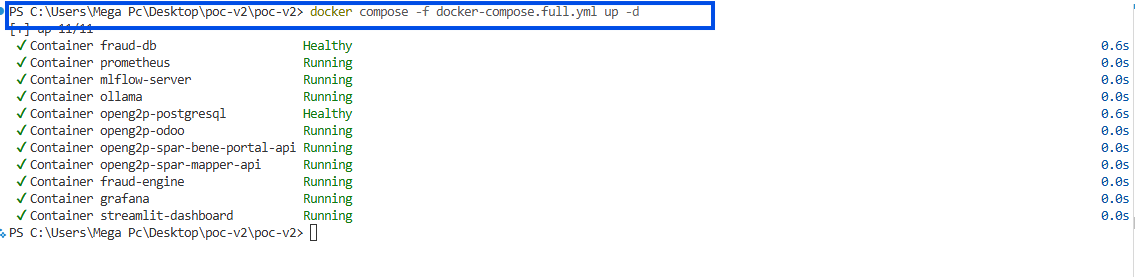
\includegraphics[width=1.2\textwidth,keepaspectratio]{DockerStart.png}
    \caption{Démarrage de l'ensemble du système via Docker Compose}
    \label{fig:docker-start}
\end{figure}


\subsection{Interface de la plateforme OpenG2P après la stabilisation}

\hspace{0.5cm}Une fois l'environnement Docker stabilisé, la plateforme OpenG2P est accessible via son interface web basée sur Odoo 17. Les captures suivantes présentent les principaux écrans utilisés au cours du projet.

\begin{figure}[H]
  \centering
  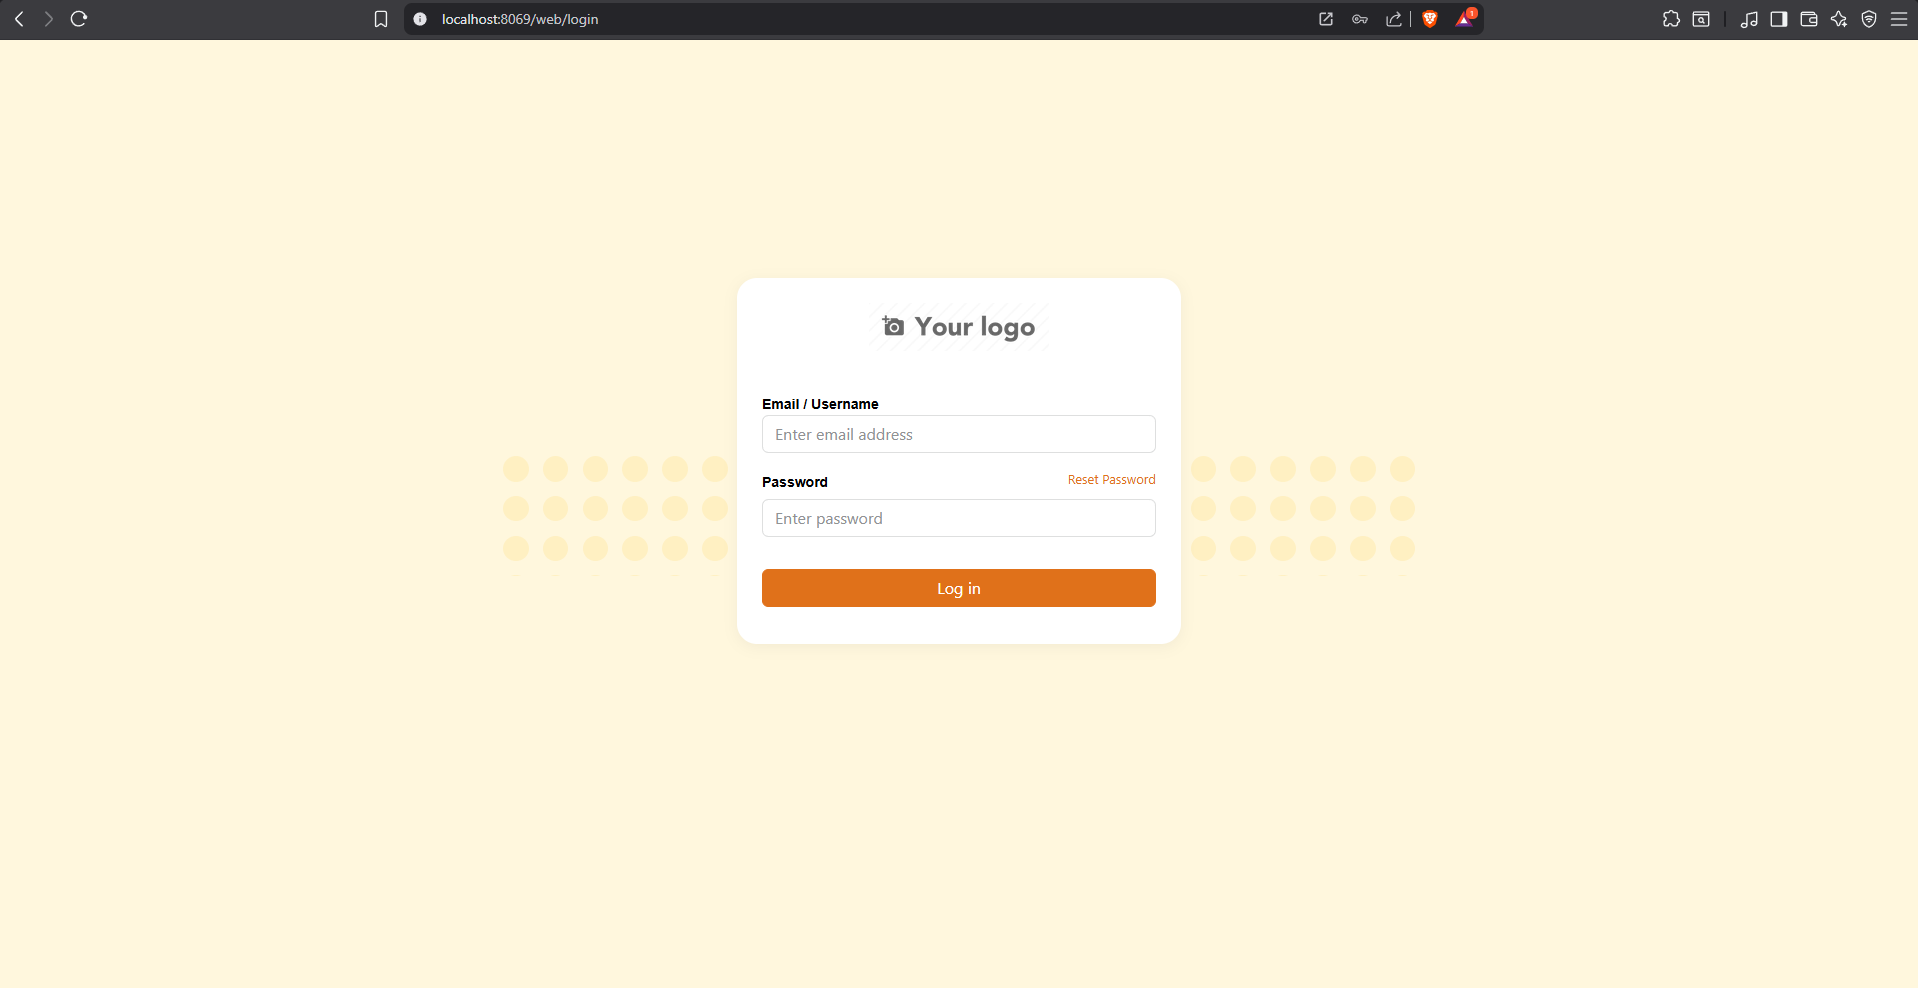
\includegraphics[width=0.92\textwidth]{openg2plogin.png}
  \caption{Écran de connexion à la plateforme OpenG2P}
\end{figure}

\hspace{0.5cm}Cet écran permet aux administrateurs de s'authentifier avant d'accéder aux fonctionnalités de la plateforme.

\begin{figure}[H]
  \centering
  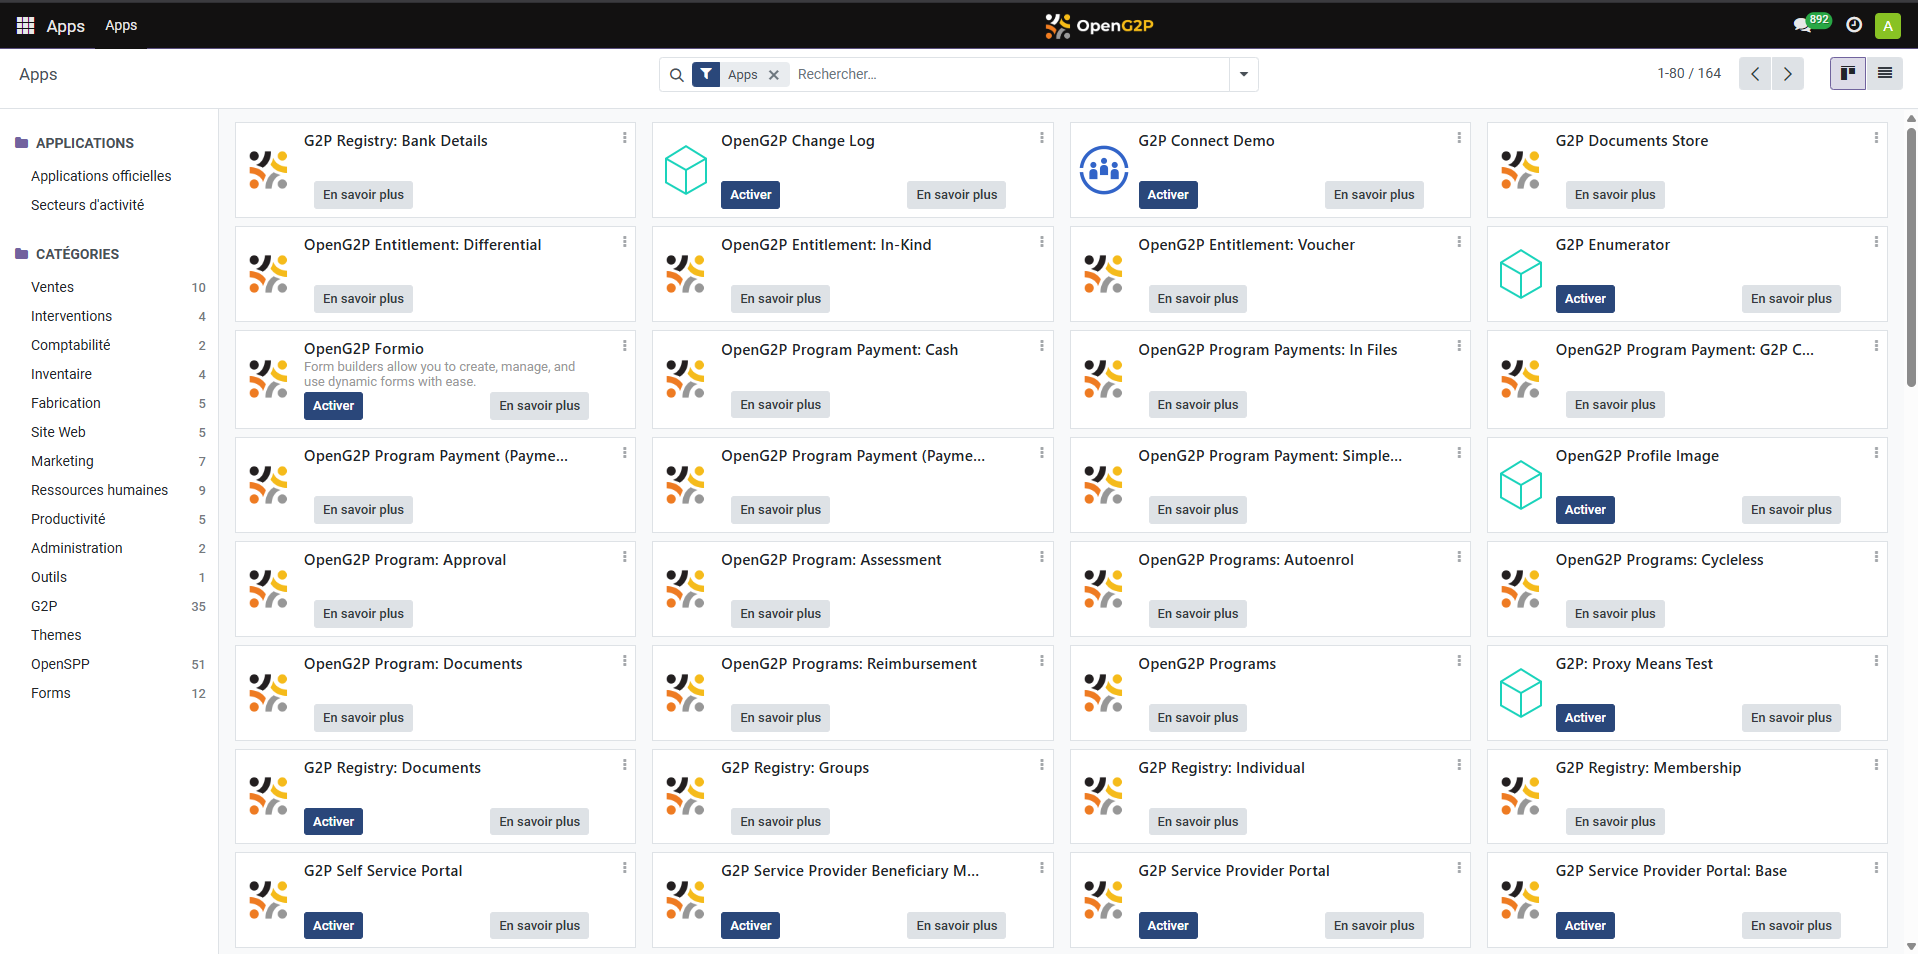
\includegraphics[width=0.92\textwidth]{modulesopeng2p.png}
  \caption{Tableau de bord principal après authentification}
\end{figure}

\hspace{0.5cm}Le tableau de bord regroupe les principaux modules disponibles pour la gestion de la protection sociale.

\begin{figure}[H]
  \centering
  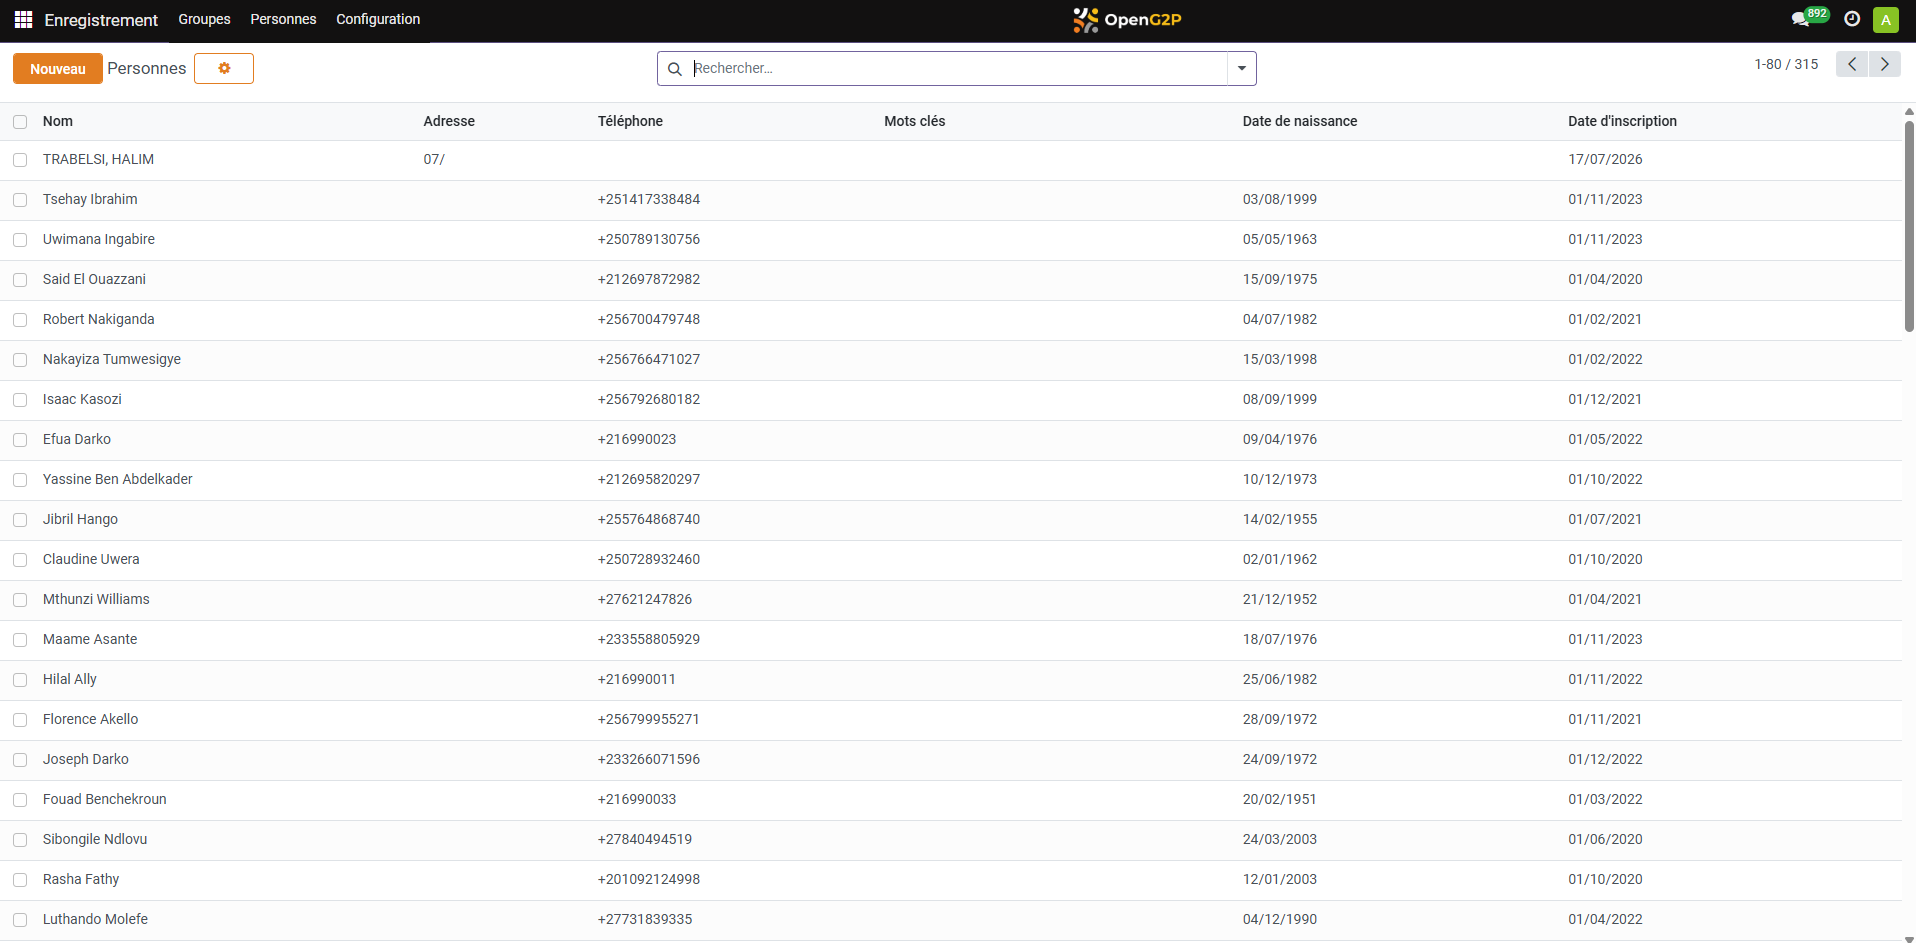
\includegraphics[width=0.92\textwidth]{OpenG2P2.png}
  \caption{Liste des bénéficiaires enregistrés dans le registre social}
\end{figure}

\hspace{0.5cm}Cette interface permet de consulter et de gérer les informations des bénéficiaires enregistrés.

\begin{figure}[H]
  \centering
  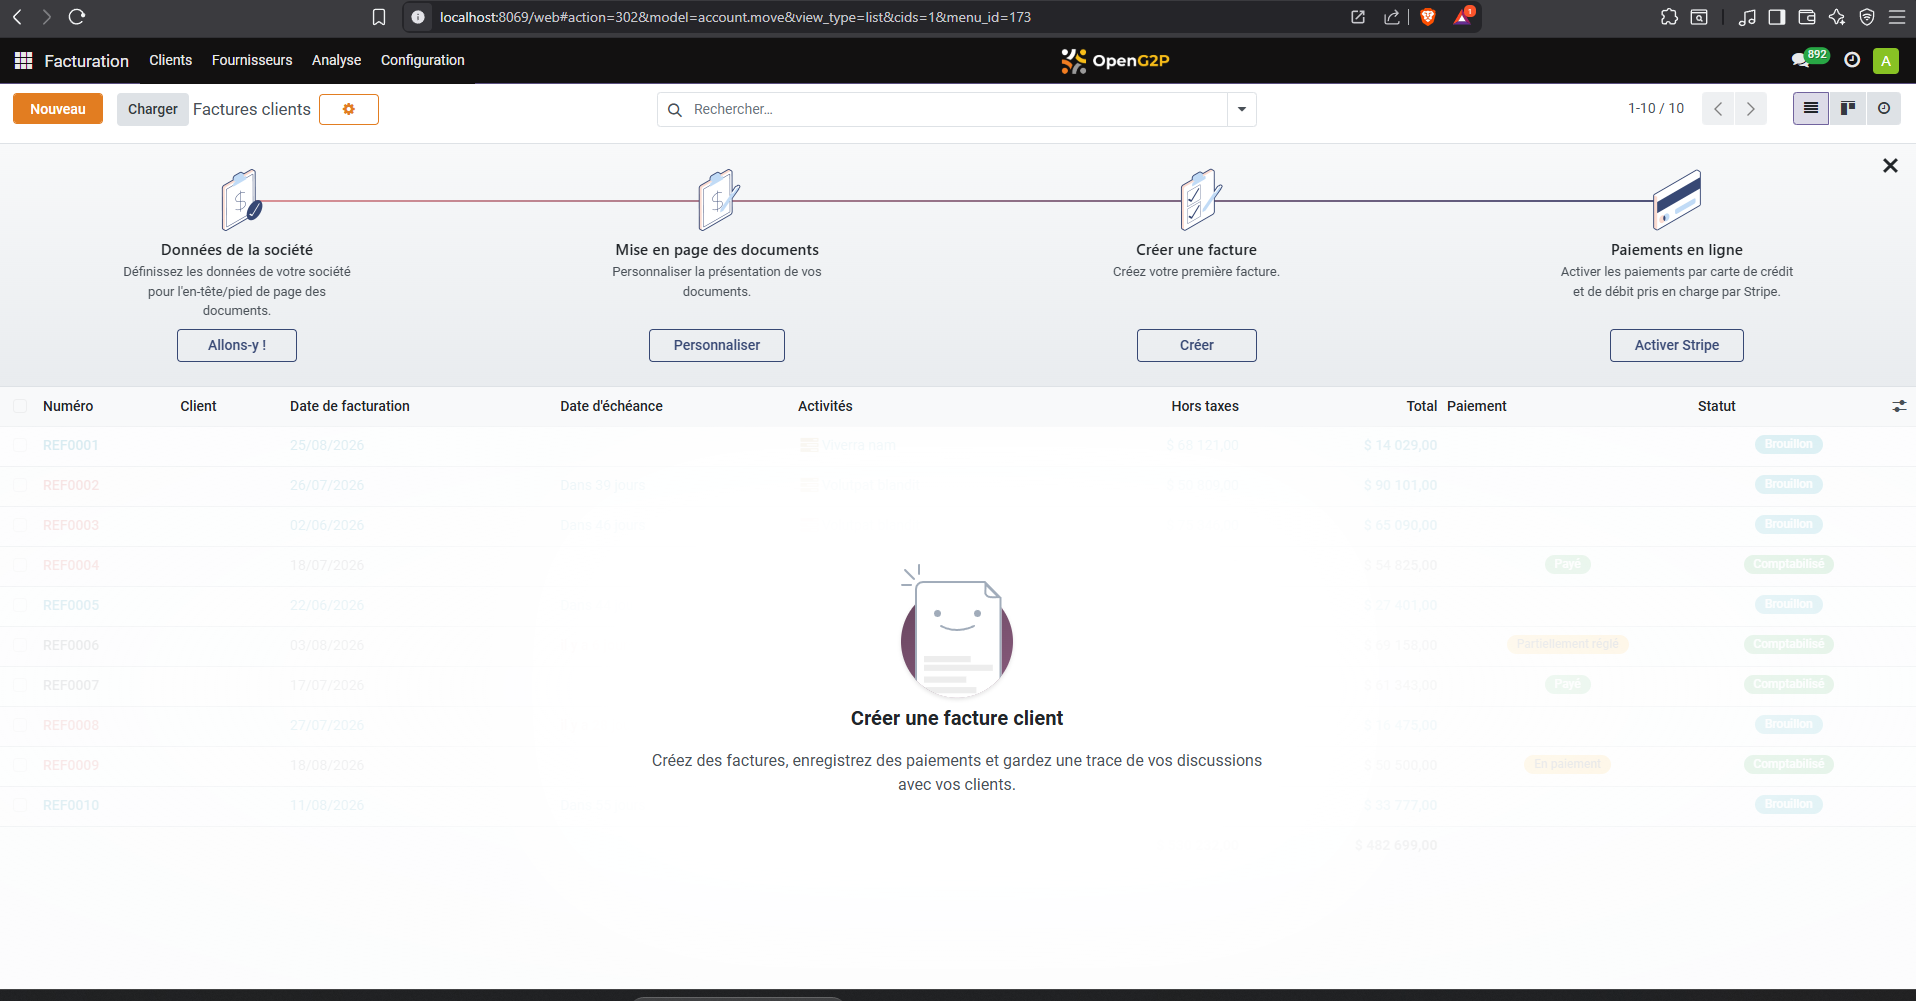
\includegraphics[width=0.92\textwidth]{facturation.png}
  \caption{Gestion des groupes de bénéficiaires}
\end{figure}

\hspace{0.5cm}Les bénéficiaires peuvent être regroupés selon différents critères pour faciliter leur administration.

\begin{figure}[H]
  \centering
  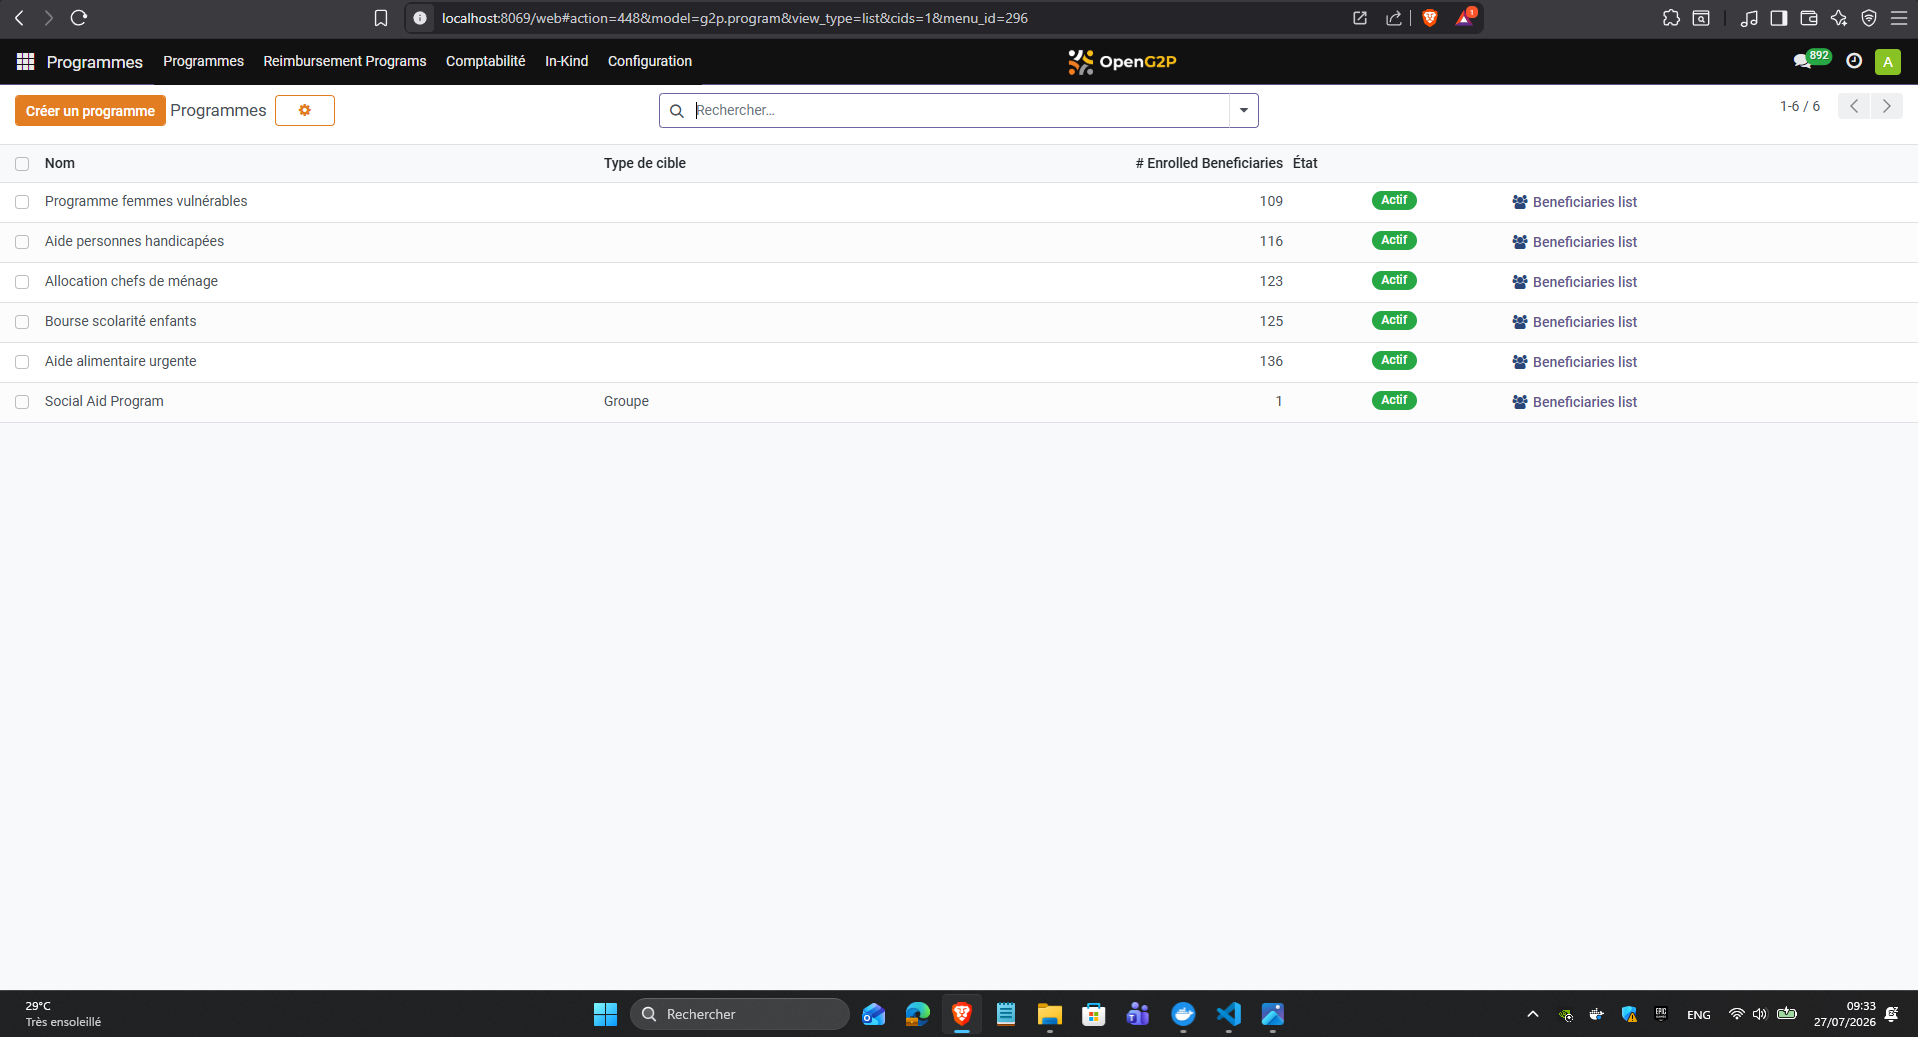
\includegraphics[width=0.92\textwidth]{openg2p_programmes.png}
  \caption{Gestion des programmes sociaux et de leurs inscriptions}
\end{figure}

\hspace{0.5cm}Cette vue permet de créer les programmes sociaux et de suivre les inscriptions des bénéficiaires.

\begin{figure}[H]
  \centering
  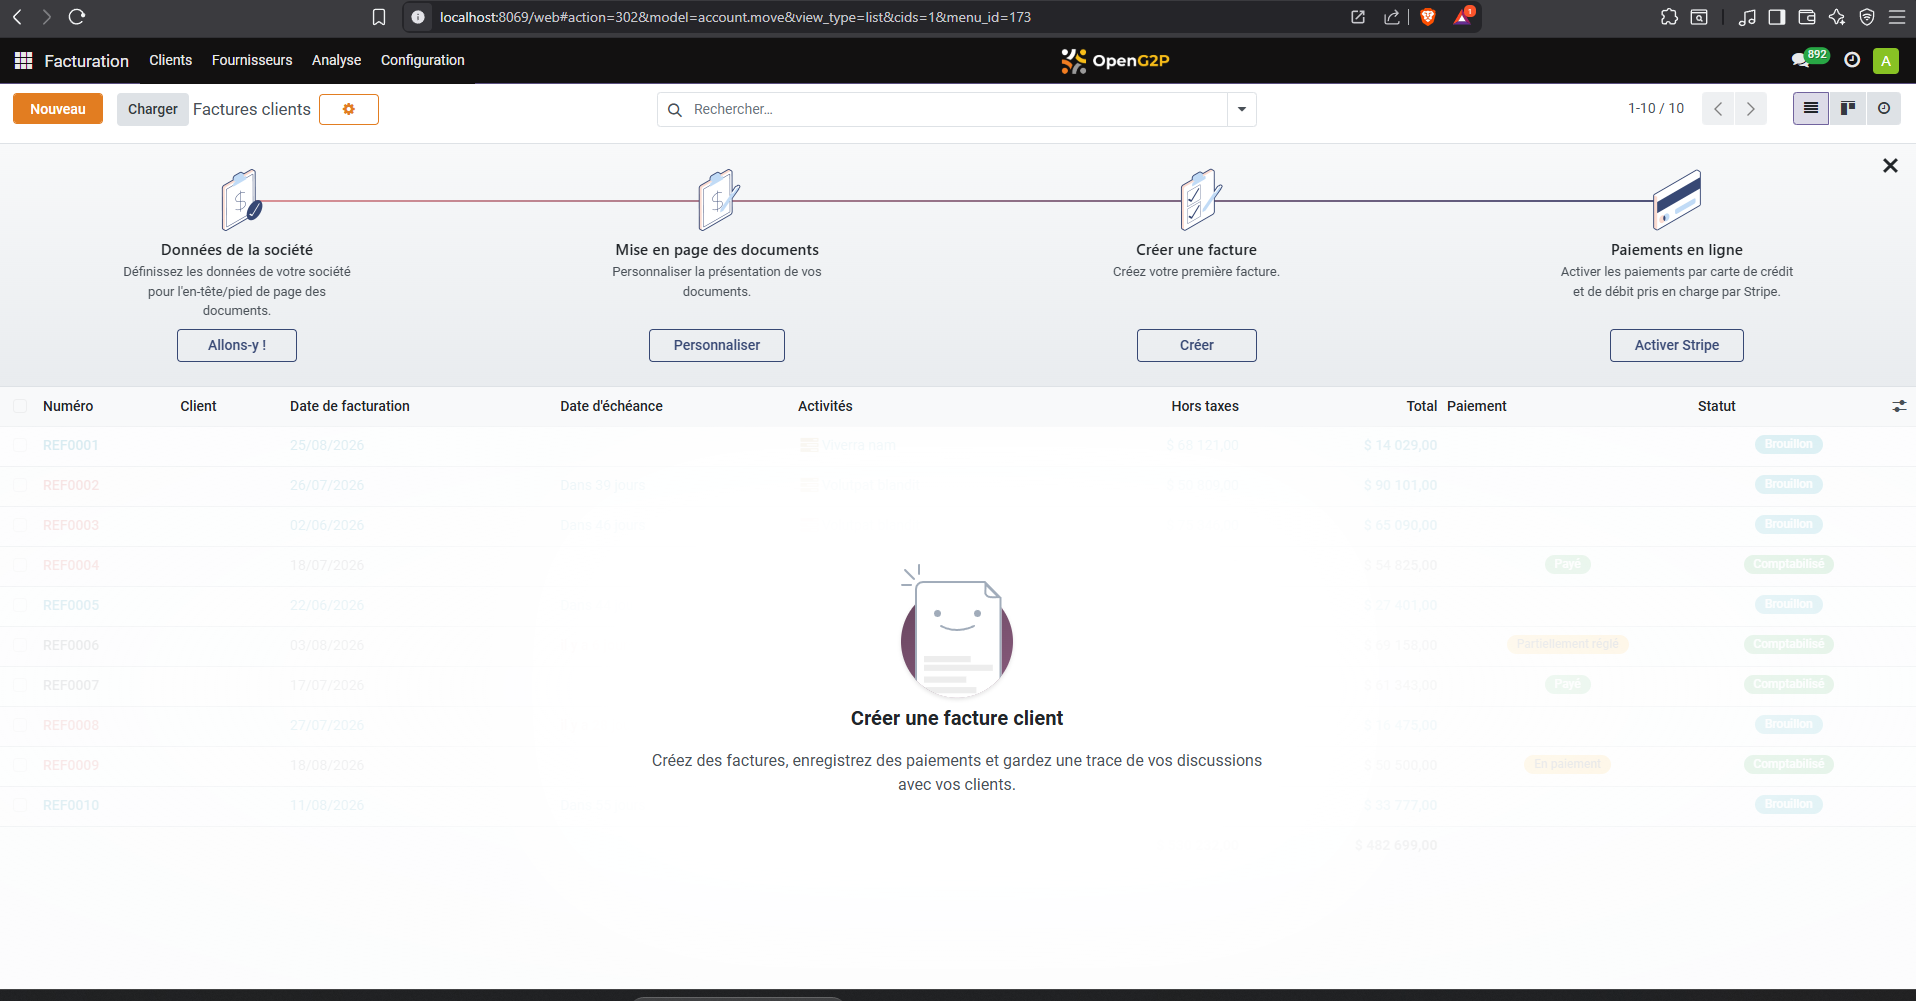
\includegraphics[width=0.92\textwidth]{facturation.png}
  \caption{Gestion des paiements et des factures}
\end{figure}

\hspace{0.5cm}Les opérations de paiement et de facturation sont centralisées dans cette interface.

\subsection{Interface de monitoring et de supervision}

\begin{figure}[H]
  \centering
  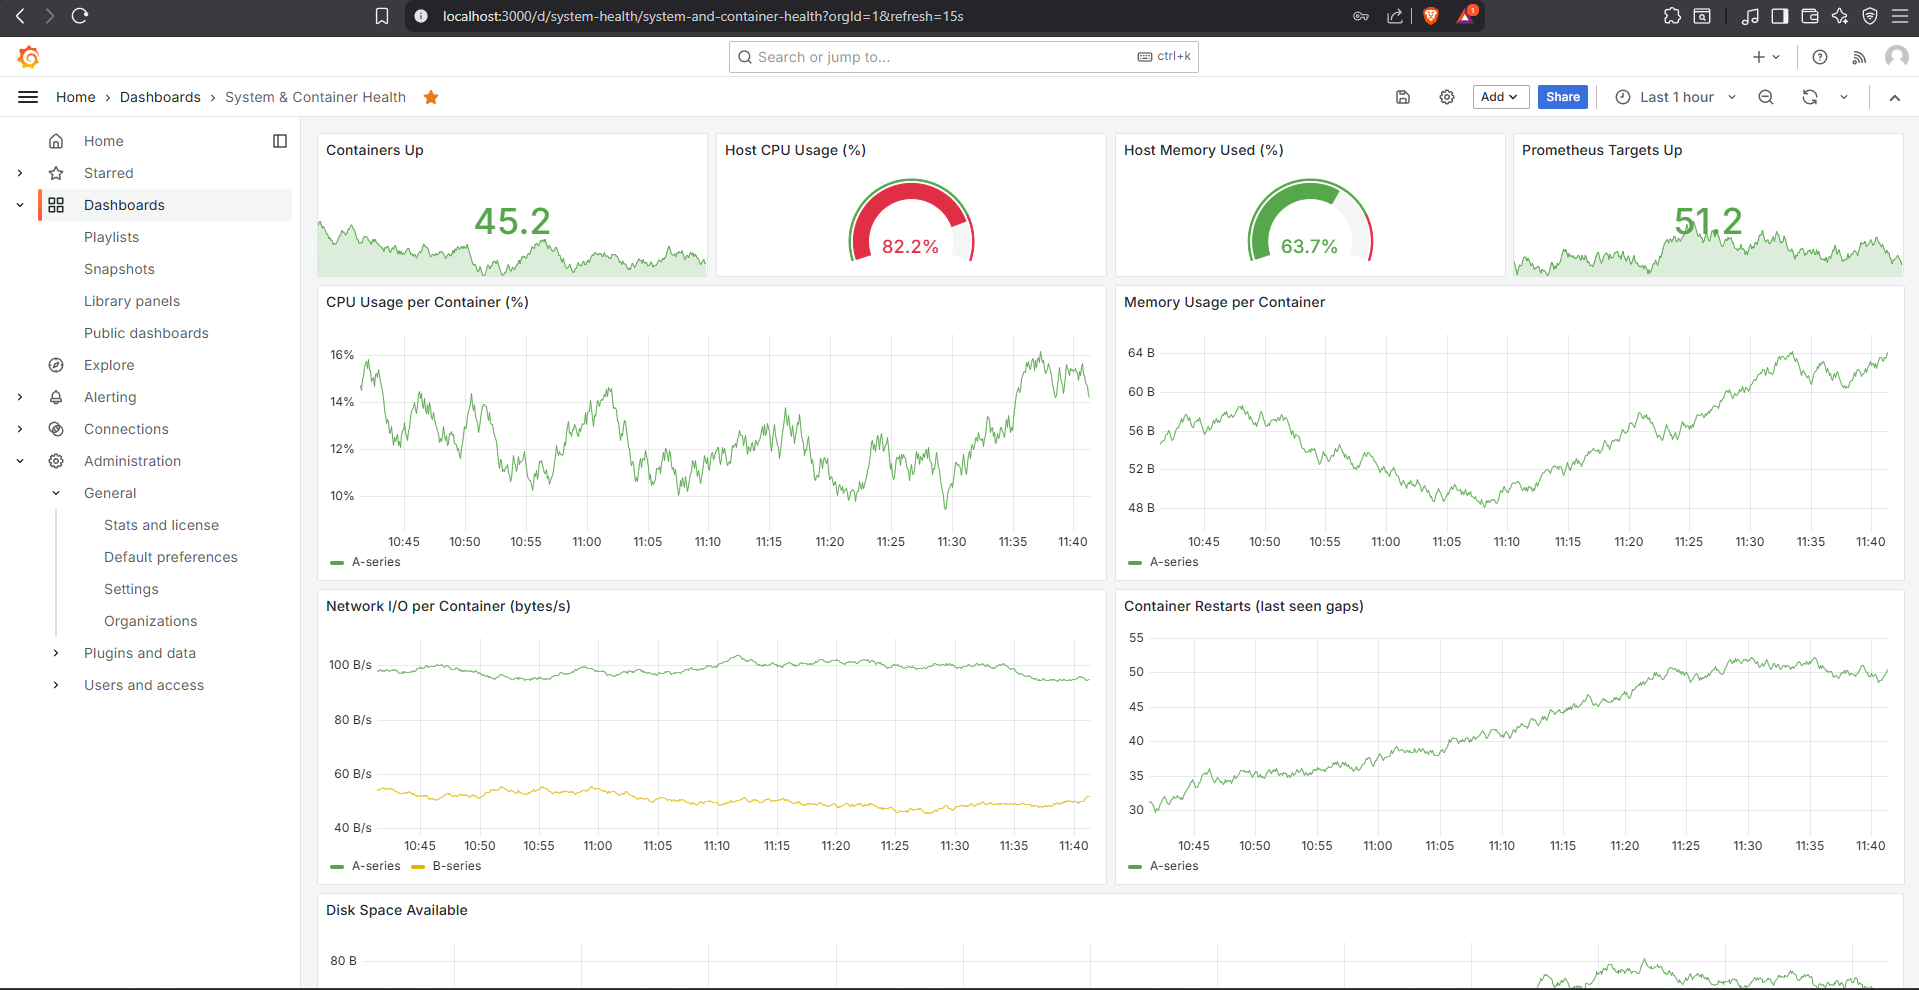
\includegraphics[width=0.92\textwidth]{GrafanaOpeng2p.png}
  \caption{Monitoring de l'état des conteneurs et des métriques système via Grafana}
\end{figure}

\hspace{0.5cm}Grafana permet de visualiser en temps réel les performances et l'état des différents services de OpenG2p.

\begin{figure}[H]
  \centering
  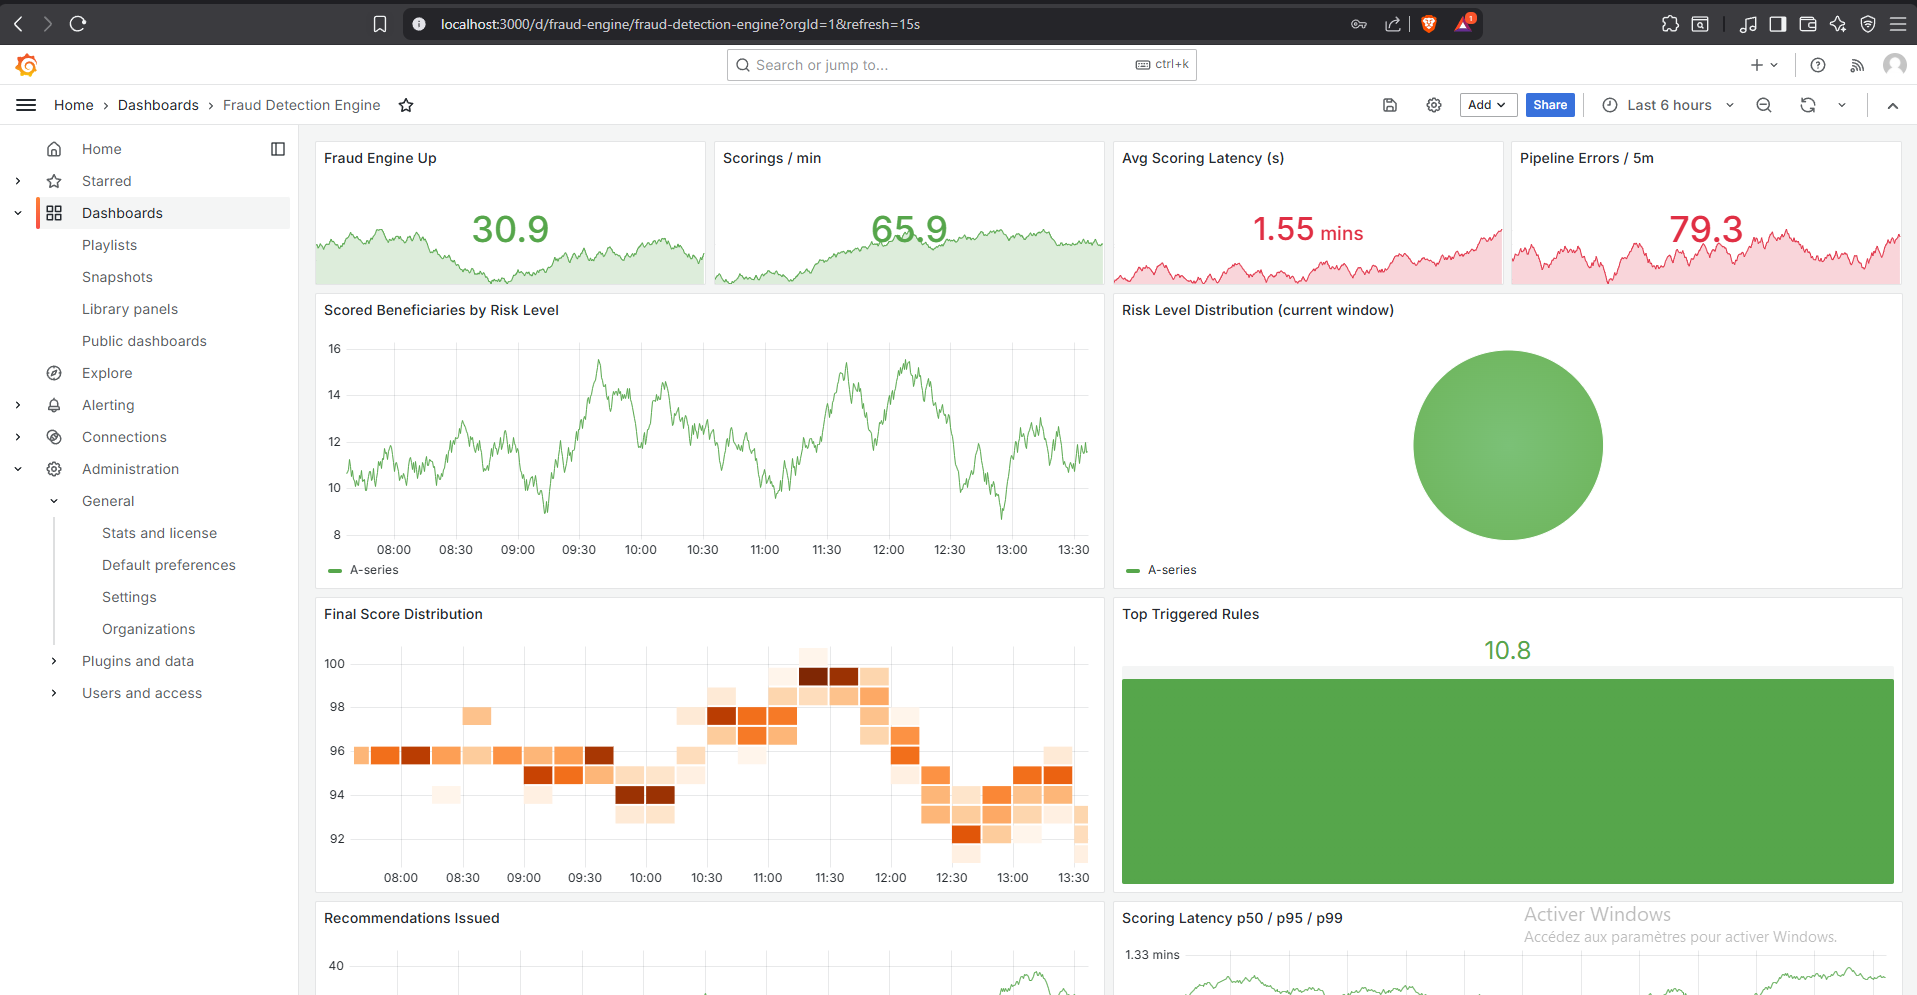
\includegraphics[width=0.92\textwidth]{GrafanaFraud.png}
  \caption{Monitoring de l'état du moteur anti-fraude via Grafana}
\end{figure}

\hspace{0.5cm}Aussi il permet de visualiser les métriques du système de détection de fraude.

\begin{figure}[H]
  \centering
  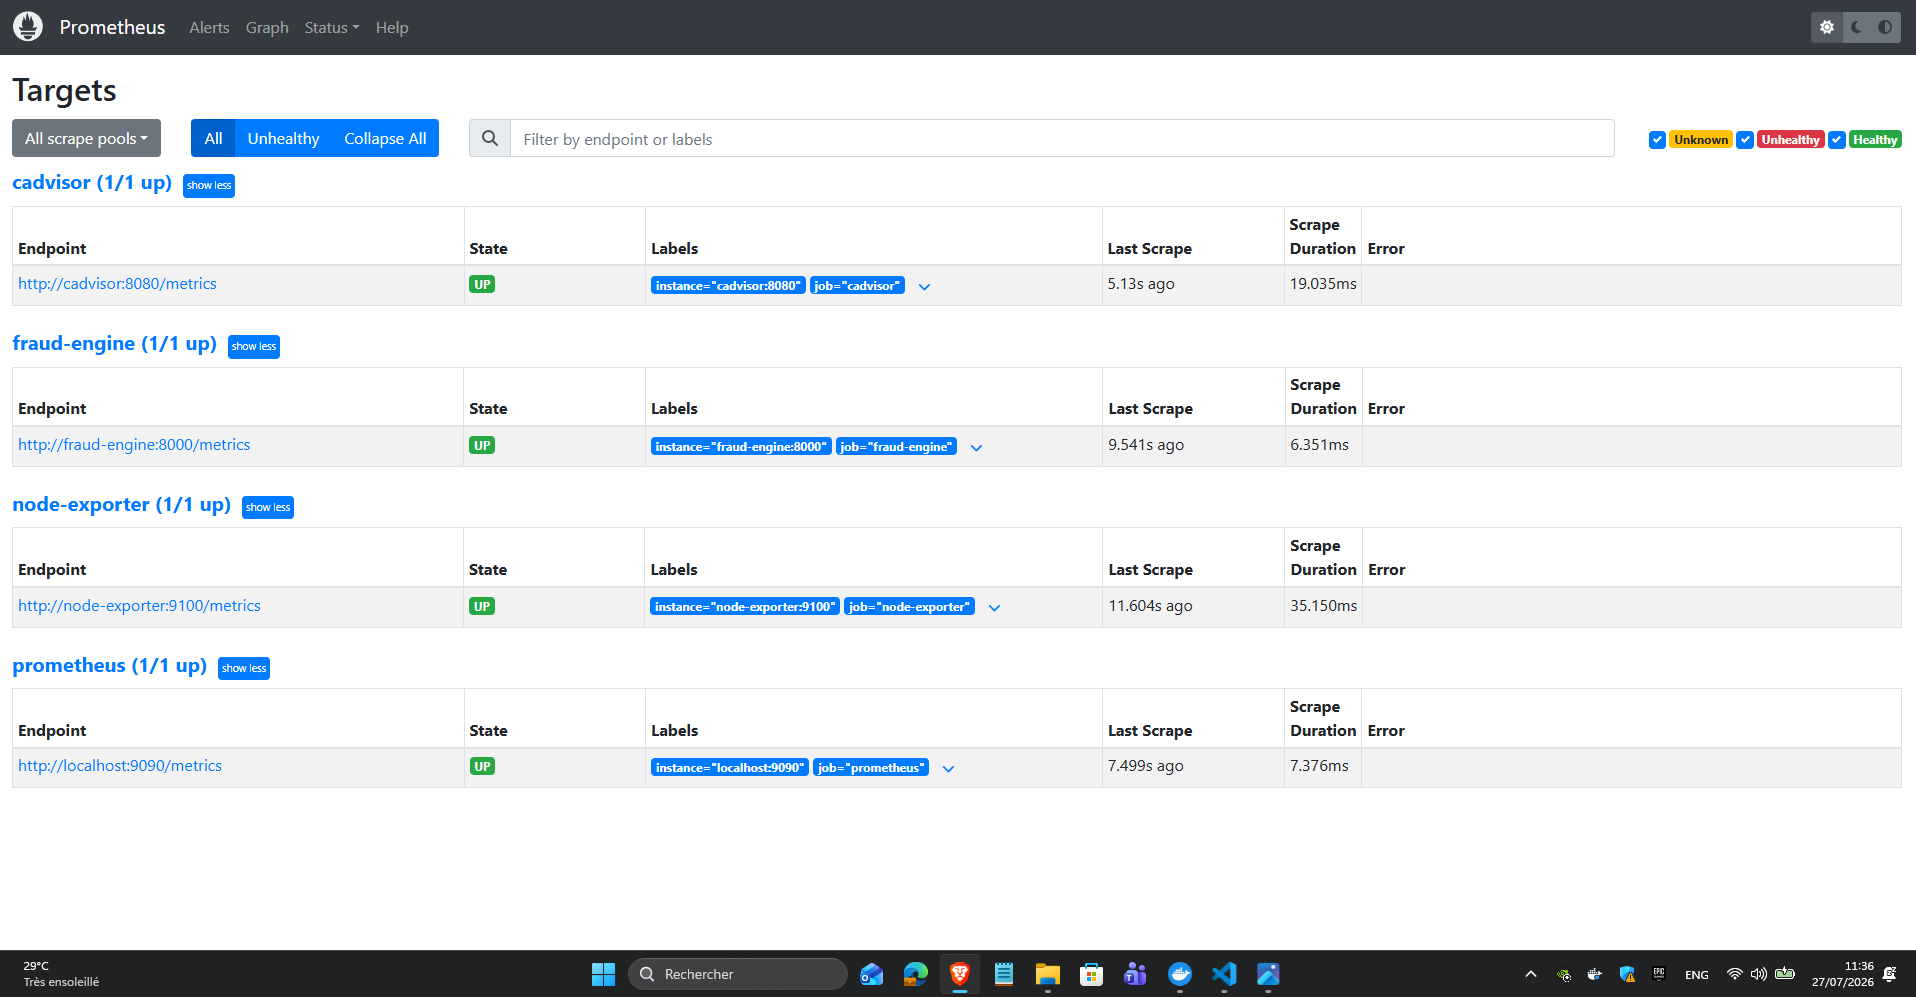
\includegraphics[width=0.92\textwidth]{PrometheusOpenG2P.png}
  \caption{Suivi de l'état des services via Prometheus}
\end{figure}

\hspace{0.5cm}Prometheus collecte les métriques des conteneurs afin d'assurer le suivi de leur disponibilité.


\newpage
% ─────────────────────────────────────────────────────────────
\section{Développement des fonctionnalités}
% ─────────────────────────────────────────────────────────────
\subsection{Construction du dataset}

\hspace{0.5cm}Le développement du moteur de détection de fraude repose sur des modèles de Machine Learning, dont les performances dépendent directement de la qualité des données utilisées pour leur apprentissage. Or, la plateforme OpenG2P ne contient pas de cas de fraude étiquetés, puisqu'elle a été conçue pour gérer les programmes de protection sociale et non pour enregistrer des fraudes. Il a donc été nécessaire de construire un jeu de données adapté afin de permettre l'entraînement et l'évaluation des modèles.

\hspace{0.5cm}Pour garantir un dataset représentatif, celui-ci a été élaboré à partir des informations disponibles dans OpenG2P. Les données des bénéficiaires ont été extraites, enrichies et organisées de manière à refléter leur situation et leurs interactions avec la plateforme. La Figure~\ref{fig:construction-dataset} présente les principales étapes de ce processus, qui seront détaillées dans les sections suivantes.

\begin{figure}[H]
  \centering
  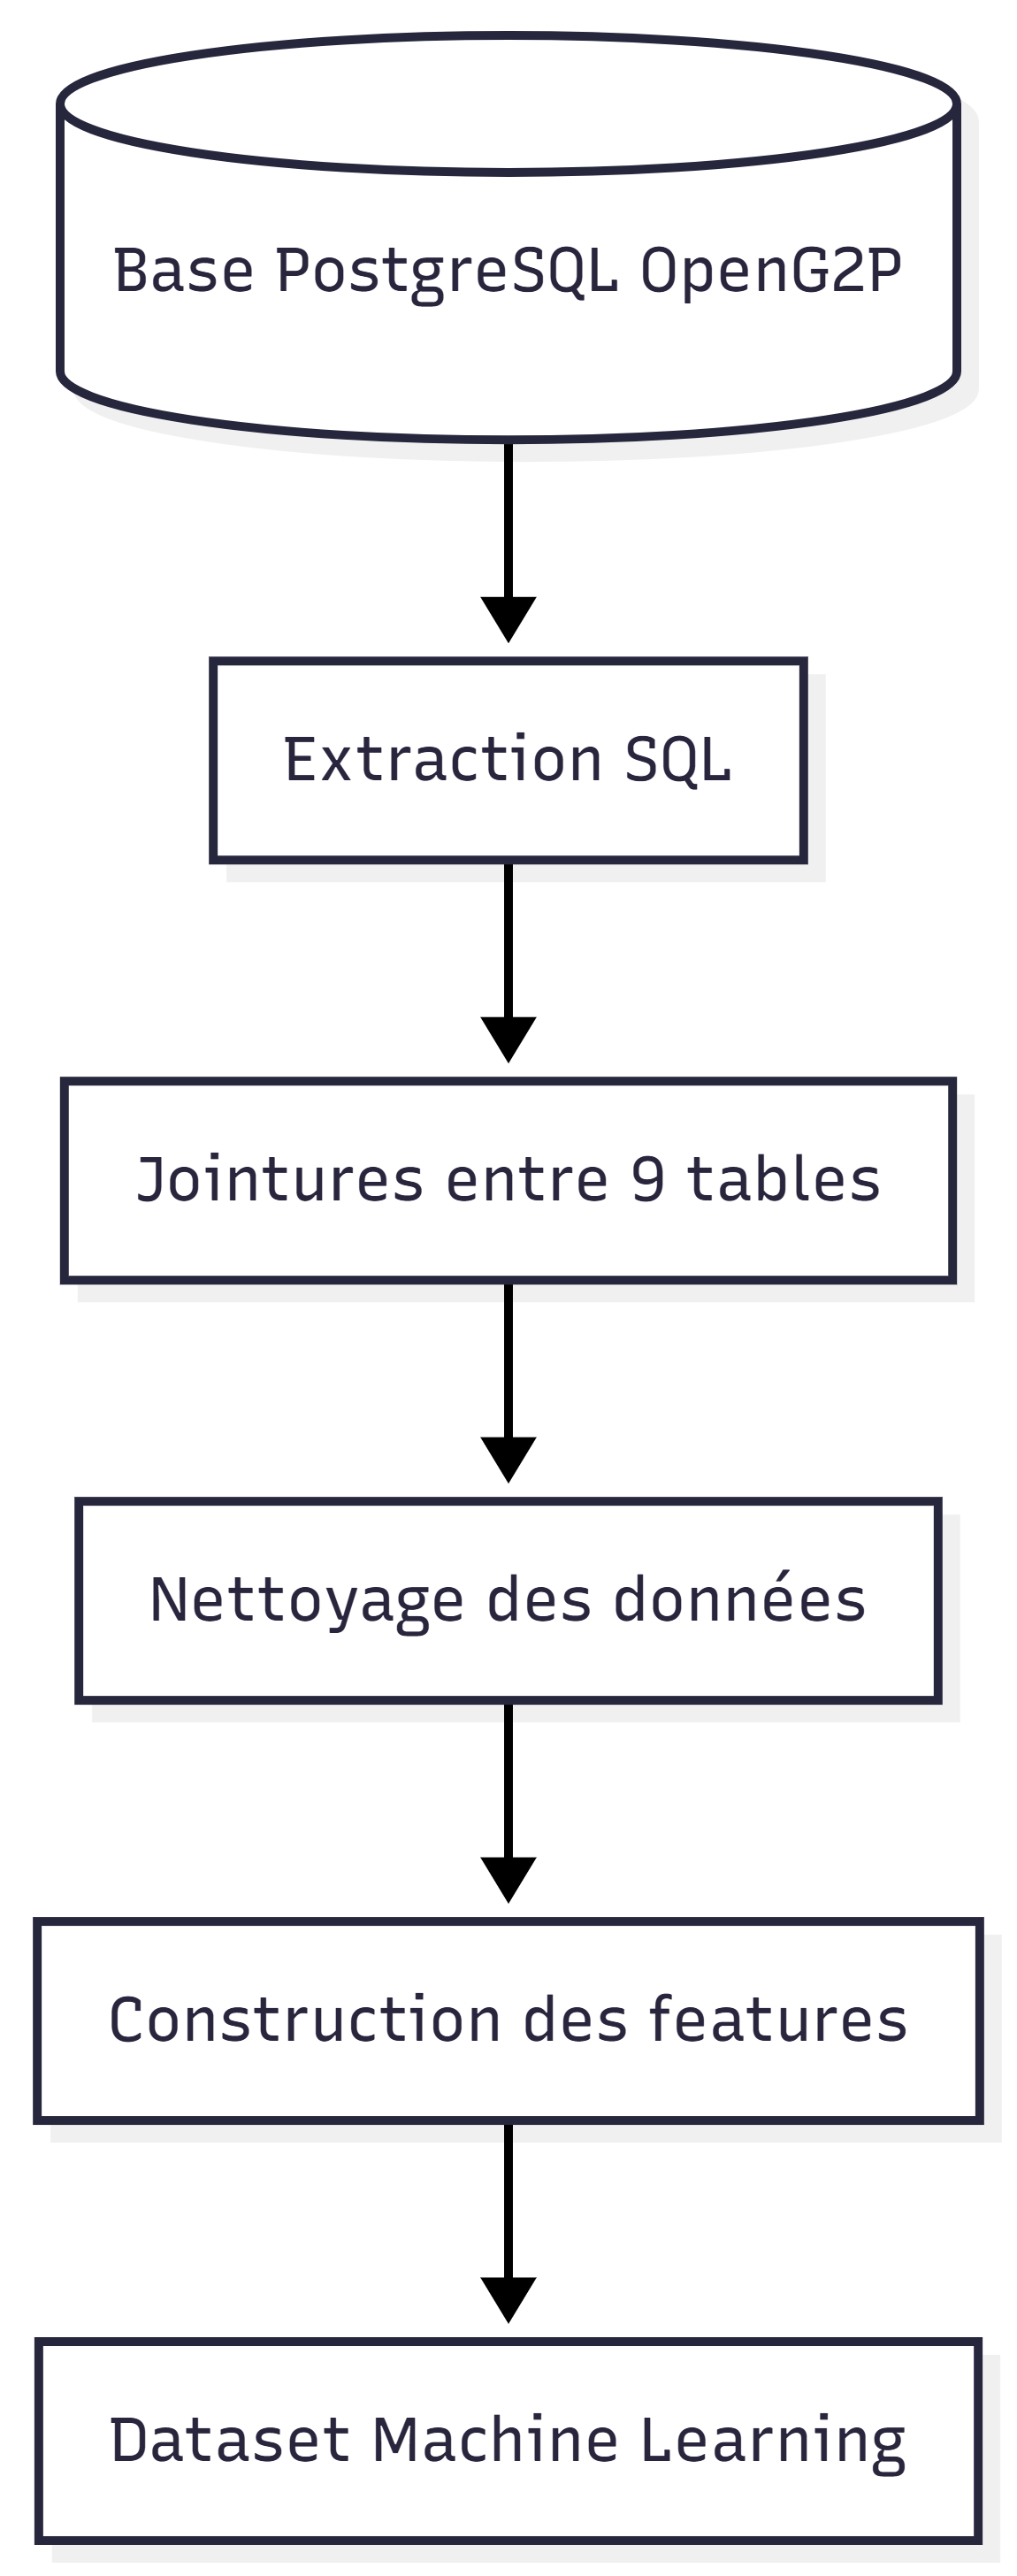
\includegraphics[width=0.2\textwidth]{Construction_dataset.png}
  \caption{Processus de construction du dataset de détection de fraude à partir des données OpenG2P}
  \label{fig:construction-dataset}
\end{figure}
\hspace{0.5cm}La construction du dataset débute par l'extraction des données depuis la base OpenG2P. Après les jointures entre les différentes tables et le nettoyage des données, les variables utiles sont construites afin d'obtenir un jeu de données prêt pour l'entraînement des modèles de Machine Learning.

\subsection{Modélisation et choix des scénarios de fraude}

\hspace{0.5cm}Avant d'extraire la moindre donnée, il fallait d'abord définir précisément l'objectif de détection~: quels comportements doivent être reconnus comme frauduleux~? Cette question a été tranchée en s'appuyant sur neuf scénarios de fraude reconnus dans la littérature sur la protection sociale, qui servent de référence pour étiqueter les exemples du dataset d'entraînement~:

\begin{figure}[H]
    \centering
    
\includegraphics[width=0.92\textwidth]{ScenarioFraude.png}
    \caption{Scénarios de fraude simulés}
    \label{fig:scenarios-fraude}
\end{figure}

\hspace{0.5cm}Le Tableau~\ref{tab:scenarios-fraude} décrit ces neuf scénarios en langage simple. Chacun correspond à une manière connue de tromper un programme d'aide sociale, allant de la fraude d'une seule personne jusqu'à la fraude organisée en réseau.

\begin{table}[H]
\centering
\caption{Description des neuf scénarios de fraude simulés}
\label{tab:scenarios-fraude}
\renewcommand{\arraystretch}{1.4}
\begin{tabular}{>{\bfseries}p{4cm} p{10.8cm}}
\hline
\thead{Scénario} & \thead{En quoi consiste la fraude} \\
\hline
\rowcolor{EYgray}
Inscriptions multiples & Le bénéficiaire s'inscrit à plusieurs programmes d'aide en même temps afin de cumuler plusieurs aides. \\
Téléphone partagé & Un même numéro de téléphone est utilisé par plusieurs bénéficiaires, ce qui indique qu'une seule personne contrôle plusieurs dossiers. \\
\rowcolor{EYgray}
Ménage fantôme & Le bénéficiaire déclare un ménage plus nombreux qu'en réalité pour toucher une aide plus élevée. \\
Manipulation des paiements & Le bénéficiaire reçoit un premier paiement puis disparaît des cycles suivants, un comportement anormal qui trahit une manipulation. \\
\rowcolor{EYgray}
Usurpation d'identité & Une identité volée ou fabriquée est utilisée pour s'inscrire au programme. \\
Sous-déclaration du revenu & Le bénéficiaire déclare un revenu bien plus faible que son revenu réel pour paraître éligible à l'aide. \\
\rowcolor{EYgray}
Fraude coordonnée & Un petit groupe de bénéficiaires partage plusieurs téléphones et comptes bancaires pour frauder ensemble. \\
Ménage fantôme systématique & De faux ménages sont créés de façon répétée et organisée, à grande échelle. \\
\rowcolor{EYgray}
Exploitation du réseau & Un grand nombre de comptes reliés entre eux (téléphones et comptes partagés) exploitent le système de manière massive. \\
\hline
\end{tabular}
\end{table}

\hspace{0.5cm}Pour rendre ce jeu de données réaliste, deux précautions ont été prises. D'abord, un léger bruit aléatoire est ajouté sur les variables sensibles (revenu, score PMT, nombre de programmes)~: sans cela, les fraudeurs et les bénéficiaires honnêtes seraient trop faciles à séparer, et le modèle donnerait de bons résultats sur ces données mais échouerait en conditions réelles. Ensuite, environ 8~\% des fraudeurs reçoivent des caractéristiques proches de celles des bénéficiaires honnêtes~: ce sont des cas volontairement difficiles, qui imitent les vrais fraudeurs cherchant à passer inaperçus.

\hspace{0.5cm}Ces neuf scénarios une fois définis, la question suivante devient celle des moyens~: quelles variables, parmi celles disponibles dans OpenG2P, permettent réellement de les détecter~?

\newpage
\subsection{Exploration de la base et extraction SQL}

\hspace{0.5cm}La difficulté centrale de cette extraction tient à la taille et à la complexité de la base OpenG2P elle-même. En tant qu'écosystème Odoo complet, elle compte plusieurs \textbf{centaines de tables} couvrant de nombreux modules sans rapport avec la détection de fraude (comptabilité, CRM, notifications, etc.), au sein desquelles il faut identifier le sous-ensemble réellement pertinent. La Figure~\ref{fig:schema-complexity} quantifie cet écart entre le schéma disponible et le schéma effectivement exploité : sur les 587 tables du schéma \texttt{public}, seules 7 sont mobilisées par l'extraction, et parmi celles-ci, seule une fraction des colonnes disponibles (par exemple 93 colonnes dans \texttt{res\_partner}) alimente réellement les 25 features du modèle.

\begin{figure}[H]
    \centering
    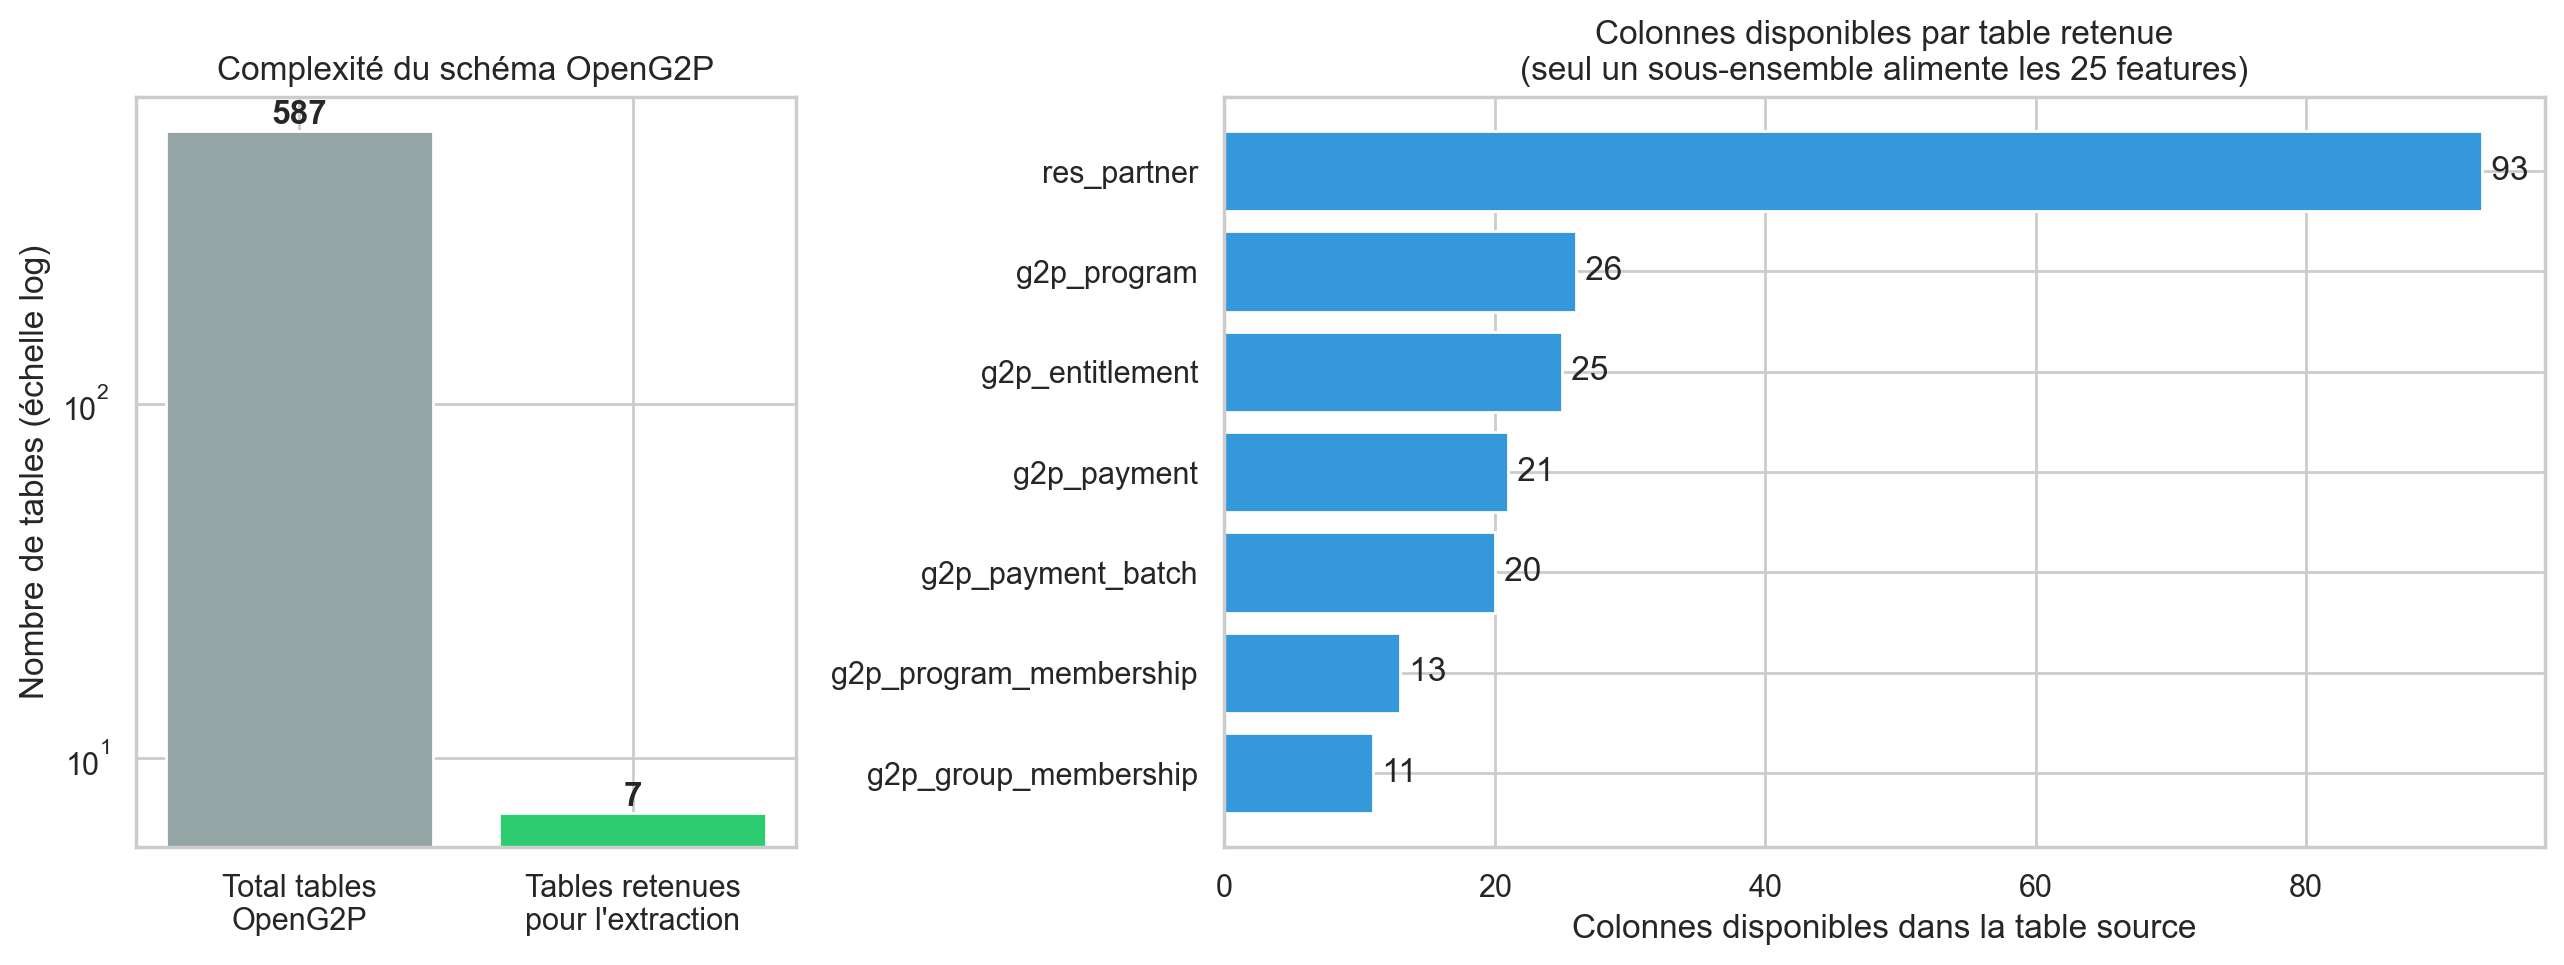
\includegraphics[width=0.92\textwidth]{openg2p_schema_complexity.png}
    \caption{Vue d'ensemble du schéma relationnel d'OpenG2P et des colonnes des sept tables sélectionnées pour l'extraction des données}
    \label{fig:schema-complexity}
\end{figure}

\hspace{0.5cm}Le module \textbf{Feature extractor} est responsable de l'extraction des informations depuis la base PostgreSQL d'OpenG2P. Afin de limiter les accès à la base de données, une requête SQL unique utilisant des Common Table Expressions (CTE) est exécutée. Cette requête réalise les jointures entre les tables retenues et agrège les informations relatives à chaque bénéficiaire en une seule ligne par profil, directement exploitable pour construire les variables d'entrée du moteur.

\subsubsection{Sélection des sources de données}

\hspace{0.5cm}La solution retenue consiste à sélectionner, parmi l'ensemble des tables OpenG2P, celles qui contiennent un signal pertinent pour caractériser le profil socio-économique d'un bénéficiaire, sa participation aux programmes sociaux et son historique de paiements. L'analyse du schéma relationnel de la base PostgreSQL a permis d'identifier les modules et tables listés au Tableau~\ref{tab:data_sources}, qui constituent les principales sources utilisées pour construire les variables d'entrée du moteur de détection de fraude.

\begin{table}[H]
\centering
\caption{Principales sources de données exploitées pour la construction du dataset}
\label{tab:data_sources}
\renewcommand{\arraystretch}{1.3}
\begin{tabular}{>{\bfseries}p{4cm} p{4cm} p{7cm}}
\hline
\thead{Module OpenG2P} & \thead{Tables principales} & \thead{Informations exploitées} \\
\hline
\rowcolor{EYgray}
Social Registry &
\texttt{res\_partner} &
Informations d'identification du bénéficiaire (âge, sexe, téléphone, compte bancaire, revenu, etc.) \\

Program Management &
\texttt{g2p\_program} \newline
\texttt{g2p\_program\_membership} &
Programmes sociaux, inscriptions, statut d'adhésion et ancienneté du bénéficiaire. \\

\rowcolor{EYgray}
Entitlements &
\texttt{g2p\_entitlement} &
Prestations attribuées aux bénéficiaires, droits ouverts et historique des allocations. \\

Paiements &
\texttt{g2p\_payment} \newline
\texttt{g2p\_payment\_batch} &
Historique des paiements, montants versés, statuts, cycles et fréquence des versements. \\

\rowcolor{EYgray}
Registre des ménages &
\texttt{g2p\_group} \newline
\texttt{g2p\_group\_members} &
Composition du ménage, liens familiaux et nombre de personnes à charge. \\

Évaluation socio-économique &
\texttt{PMT Assessment} &
Score PMT (Proxy Means Test) utilisé pour estimer le niveau de vulnérabilité des bénéficiaires. \\
\hline
\end{tabular}
\end{table}

\hspace{0.5cm}Ces six sources couvrent l'identité du bénéficiaire, son inscription aux programmes, ses prestations, ses paiements, la composition de son ménage et son évaluation socio-économique — soit l'ensemble des dimensions nécessaires pour détecter aussi bien une fraude individuelle (revenus sous-déclarés) qu'une fraude organisée (réseau de comptes ou téléphones partagés). Ces variables sélectionnées, il reste à les transformer en un dataset structuré, directement exploitable par les algorithmes de Machine Learning.

\subsubsection{Construction des features et tableau des 25 variables}

\hspace{0.5cm}À l'issue du prétraitement, chaque profil de bénéficiaire est traduit en un vecteur de 25 features numériques, résumées par catégorie au Tableau~\ref{tab:features}. Ces variables couvrent la démographie, la composition du ménage, la participation aux programmes, le score PMT, l'historique de paiements, les signaux réseau et des indicateurs dérivés (flags).

\begin{table}[H]
\centering
\caption{Les 25 features extraites pour le modèle ML}
\label{tab:features}
\renewcommand{\arraystretch}{1.3}
\begin{tabular}{>{\bfseries}p{2.5cm} p{5cm} p{6cm}}
\hline
\thead{Catégorie} & \thead{Features} & \thead{Signification} \\
\hline
\rowcolor{EYgray}
Démographie & \texttt{age}, \texttt{income}, \texttt{income\_per\_person} & Âge, revenu total et revenu par personne \\
Ménage & \texttt{household\_size}, \texttt{nb\_children}, \texttt{nb\_elderly}, \texttt{dependency\_ratio} & Composition et vulnérabilité du ménage \\
\rowcolor{EYgray}
Ménage & \texttt{has\_disabled}, \texttt{single\_head} & Présence d'handicap, chef de ménage seul \\
Programmes & \texttt{nb\_programs}, \texttt{nb\_active\_programs}, \texttt{avg\_enrollment\_days} & Inscriptions actives et ancienneté \\
\rowcolor{EYgray}
Score PMT & \texttt{pmt\_score}, \texttt{pmt\_score\_min} & Score de ciblage proxy-means test \\
Paiements & \texttt{payment\_count}, \texttt{payment\_gap\_ratio}, \texttt{payment\_success\_rate} & Volume et taux d'échec des paiements \\
\rowcolor{EYgray}
Paiements & \texttt{amount\_variance}, \texttt{cycle\_count} & Variabilité des montants reçus \\
Réseau & \texttt{shared\_phone\_count}, \texttt{shared\_account\_count}, \texttt{network\_risk} & Partage de ressources entre bénéficiaires \\
\rowcolor{EYgray}
Groupe & \texttt{group\_membership\_count} & Appartenance à des groupes ménagers \\
Flags & \texttt{high\_amount\_flag}, \texttt{income\_program\_inconsistency} & Signaux dérivés de règles heuristiques \\
\hline
\end{tabular}
\end{table}

\hspace{0.5cm}Au-delà de ce regroupement par catégorie métier, un audit technique du schéma réel du dataset confirme la cohérence des types de données~: les 25 features sont toutes numériques (entiers, flottants ou booléens), sans valeur manquante, ce qui les rend directement exploitables par les modèles de Machine Learning sans étape d'encodage supplémentaire. Une fois ces variables construites, il reste à les assembler en un dataset tabulaire cohérent, avant de pouvoir les générer à grande échelle et les injecter dans OpenG2P.

\subsection{Structure du dataset final}

\hspace{0.5cm}À l'issue des différentes étapes d'extraction, de nettoyage et de construction des features, les informations relatives à chaque bénéficiaire sont regroupées dans un dataset tabulaire destiné à l'entraînement et à l'évaluation des modèles de détection de fraude.

\hspace{0.5cm}Le dataset obtenu est organisé sous forme tabulaire, où chaque ligne représente un bénéficiaire et chaque colonne une information descriptive ou une feature calculée. Il comporte 59 colonnes, dont 28 features utilisées par les modèles de Machine Learning, les autres étant dédiées aux identifiants et aux informations de supervision. La Figure~\ref{fig:openg2p-dtypes} présente la structure complète de ce dataset.

\begin{figure}[H]
    \centering
    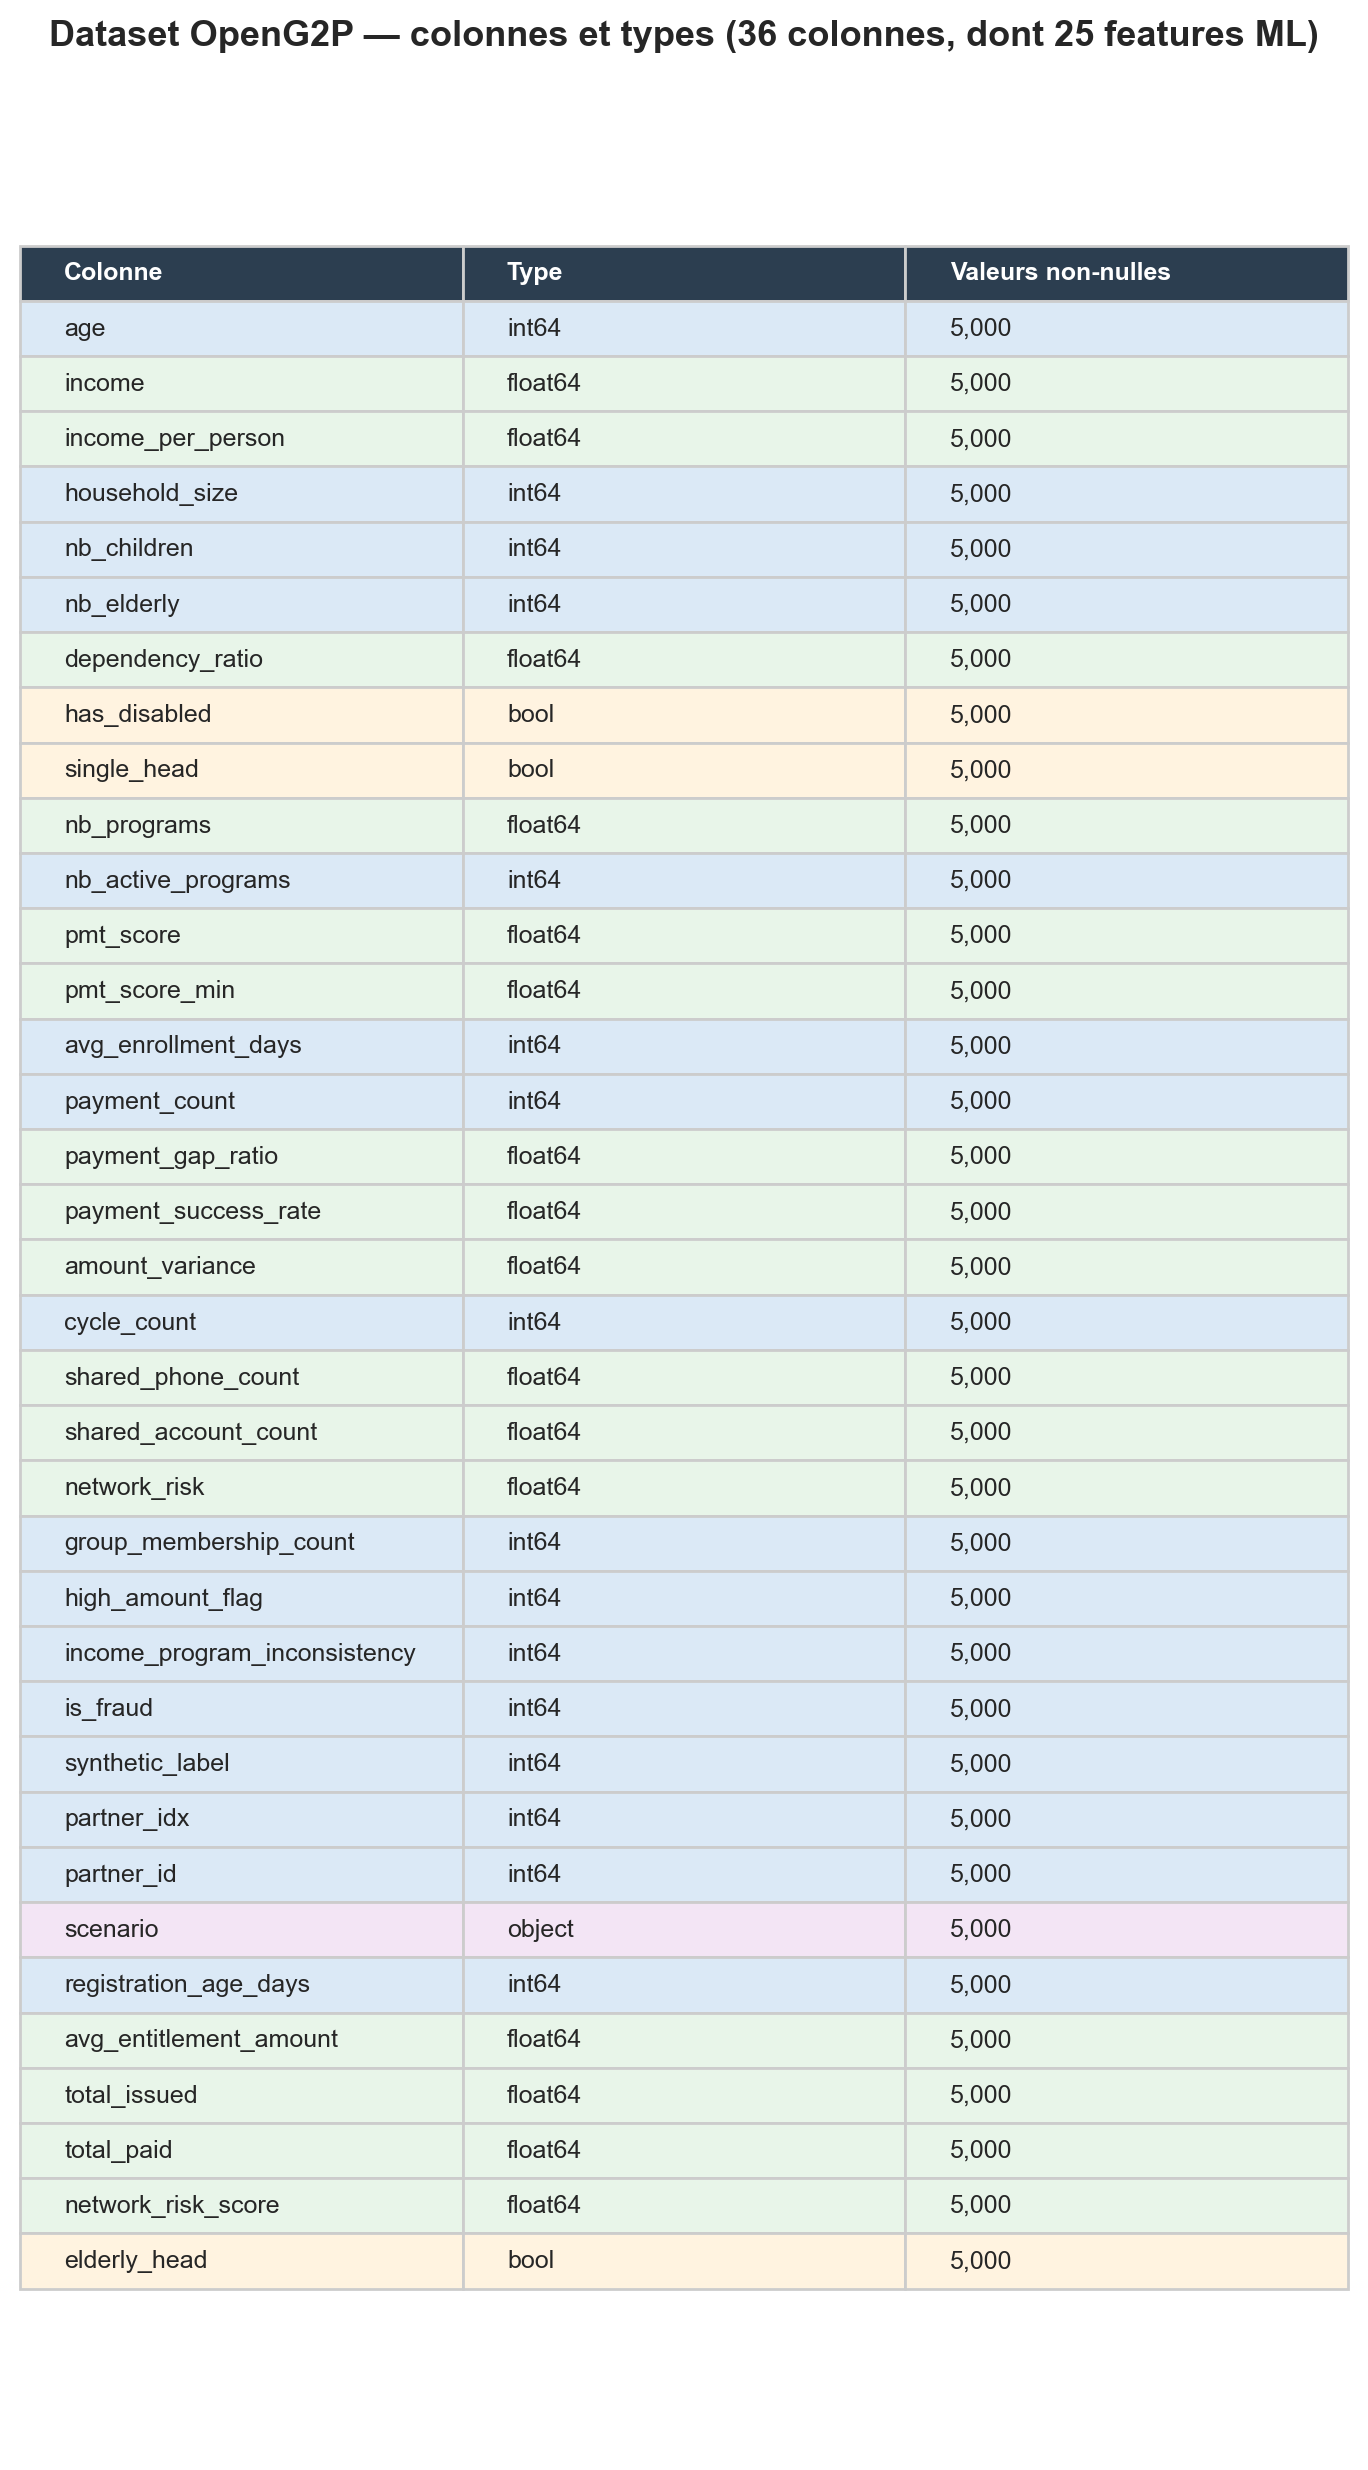
\includegraphics[width=0.85\textwidth]{openg2p_columns_dtypes.png}
    \caption{Colonnes et types du dataset OpenG2P généré (59 colonnes, dont les 28 features ML)}
    \label{fig:openg2p-dtypes}
\end{figure}

\hspace{0.5cm}Au-delà de cette vue par colonnes, une \textit{datacard} — fiche technique résumant la forme et les statistiques descriptives du dataset — a été générée automatiquement à partir du fichier réellement produit, de sorte qu'elle reste exacte à chaque régénération du dataset plutôt que d'être recopiée à la main. Le Tableau~\ref{tab:datacard-summary} en résume la forme globale, et le Tableau~\ref{tab:datacard-features} détaille les statistiques descriptives (moyenne, écart-type, minimum, maximum) de chaque feature, regroupées par catégorie.

% Auto-généré par ml/scripts/generate_datacard.py — ne pas éditer à la main.
\begin{table}[H]
\centering
\caption{Fiche technique (datacard) du dataset synthétique}
\label{tab:datacard-summary}
\renewcommand{\arraystretch}{1.4}
\begin{tabular}{>{\bfseries}p{5cm} p{9cm}}
\hline
\thead{Caractéristique} & \thead{Valeur} \\
\hline
\rowcolor{EYgray}
Nombre de lignes (bénéficiaires) & 5\,000 \\
Nombre total de colonnes & 59 \\
\rowcolor{EYgray}
Nombre de features ML & 28 \\
Types de colonnes & float64: 22, int64: 17, object: 17, bool: 3 \\
\rowcolor{EYgray}
Valeurs manquantes (sur les 28 features ML) & 0 \\
Bénéficiaires légitimes & 4\,341 \\
\rowcolor{EYgray}
Bénéficiaires frauduleux & 659 \\
Taux de fraude & 13.18~\% \\
\hline
\end{tabular}
\end{table}

\begin{table}[H]
\centering
\caption{Statistiques descriptives des features par catégorie}
\label{tab:datacard-features}
\renewcommand{\arraystretch}{1.3}
\begin{tabular}{>{\bfseries}p{3.2cm} p{3.3cm} p{2cm} p{2cm} p{2cm} p{2cm}}
\hline
\thead{Catégorie} & \thead{Feature} & \thead{Moy.} & \thead{Écart-t.} & \thead{Min} & \thead{Max} \\
\hline
\rowcolor{EYgray}
Démographie & \texttt{age} & 49.303 & 15.73 & 23.0 & 76.0 \\
 & \texttt{income} & 845.516 & 765.732 & 19.74 & 5917.09 \\
\rowcolor{EYgray}
 & \texttt{income\_per\_person} & 292.456 & 393.201 & 1.62 & 4862.12 \\
Ménage & \texttt{household\_size} & 4.374 & 2.724 & 1.0 & 21.0 \\
\rowcolor{EYgray}
 & \texttt{nb\_children} & 1.16 & 1.512 & 0.0 & 12.0 \\
 & \texttt{nb\_elderly} & 0.205 & 0.427 & 0.0 & 2.0 \\
\rowcolor{EYgray}
 & \texttt{dependency\_ratio} & 0.72 & 1.077 & 0.0 & 11.0 \\
 & \texttt{has\_disabled} & 0.071 & 0.257 & 0.0 & 1.0 \\
\rowcolor{EYgray}
 & \texttt{single\_head} & 0.156 & 0.363 & 0.0 & 1.0 \\
Programmes & \texttt{nb\_programs} & 2.053 & 1.123 & 0.0 & 6.101 \\
\rowcolor{EYgray}
 & \texttt{nb\_active\_programs} & 1.937 & 0.874 & 1.0 & 4.0 \\
 & \texttt{avg\_enrollment\_days} & 1685.972 & 420.67 & 969.0 & 2399.0 \\
\rowcolor{EYgray}
Score PMT & \texttt{pmt\_score} & 0.579 & 0.242 & 0.0 & 1.357 \\
 & \texttt{pmt\_score\_min} & 0.537 & 0.192 & 0.05 & 0.999 \\
\rowcolor{EYgray}
Paiements & \texttt{payment\_count} & 5.812 & 2.623 & 3.0 & 12.0 \\
 & \texttt{payment\_gap\_ratio} & 0.331 & 0.213 & 0.0 & 1.206 \\
\rowcolor{EYgray}
 & \texttt{payment\_success\_rate} & 0.676 & 0.139 & 0.0 & 0.917 \\
 & \texttt{amount\_variance} & 22934.443 & 14430.672 & 2034.12 & 61320.62 \\
\rowcolor{EYgray}
 & \texttt{cycle\_count} & 3.0 & 0.0 & 3.0 & 3.0 \\
Réseau & \texttt{shared\_phone\_count} & 0.846 & 1.215 & 0.0 & 9.692 \\
\rowcolor{EYgray}
 & \texttt{shared\_account\_count} & 0.632 & 0.893 & 0.0 & 6.736 \\
 & \texttt{network\_risk} & 0.178 & 0.215 & 0.0 & 1.524 \\
\rowcolor{EYgray}
Groupe & \texttt{group\_membership\_count} & 0.507 & 0.5 & 0.0 & 1.0 \\
Signaux dérivés (flags) & \texttt{high\_amount\_flag} & 0.05 & 0.218 & 0.0 & 1.0 \\
\rowcolor{EYgray}
 & \texttt{income\_program\_inconsistency} & 0.027 & 0.162 & 0.0 & 1.0 \\
Calibration économique & \texttt{income\_ratio\_to\_national} & 1.46 & 1.323 & 0.034 & 10.22 \\
\rowcolor{EYgray}
 & \texttt{household\_size\_deviation} & 0.374 & 2.724 & -3.0 & 17.0 \\
Identité & \texttt{duplicate\_national\_id\_count} & 0.005 & 0.072 & 0.0 & 1.0 \\
\hline
\end{tabular}
\end{table}

\hspace{0.5cm}Ce dataset structuré n'a de valeur que s'il peut être produit à l'échelle et alimenter réellement la plateforme~: c'est l'objet de la dernière étape de cette construction.

\newpage
\subsection{Génération du dataset synthétique et injection PostgreSQL}

\hspace{0.5cm}Une fois les différentes features définies, un module dédié génère automatiquement un grand nombre de profils synthétiques reproduisant les principales caractéristiques observées dans les données OpenG2P : démographie, composition des ménages, historique des paiements et relations entre bénéficiaires. Ces profils sont ensuite injectés directement dans la base PostgreSQL d'OpenG2P afin d'obtenir un environnement de test réaliste, suffisamment riche pour entraîner et évaluer les modèles, sans utiliser de données personnelles réelles.

\hspace{0.5cm}La Figure~\ref{fig:generation-dataset} présente ce processus. À partir de plusieurs scénarios de fraude et de profils légitimes définis lors de la phase de conception, le générateur crée automatiquement les bénéficiaires synthétiques puis les insère dans les différentes tables d'OpenG2P en respectant les relations et les contraintes de la base de données.

\begin{figure}[H]
    \centering
    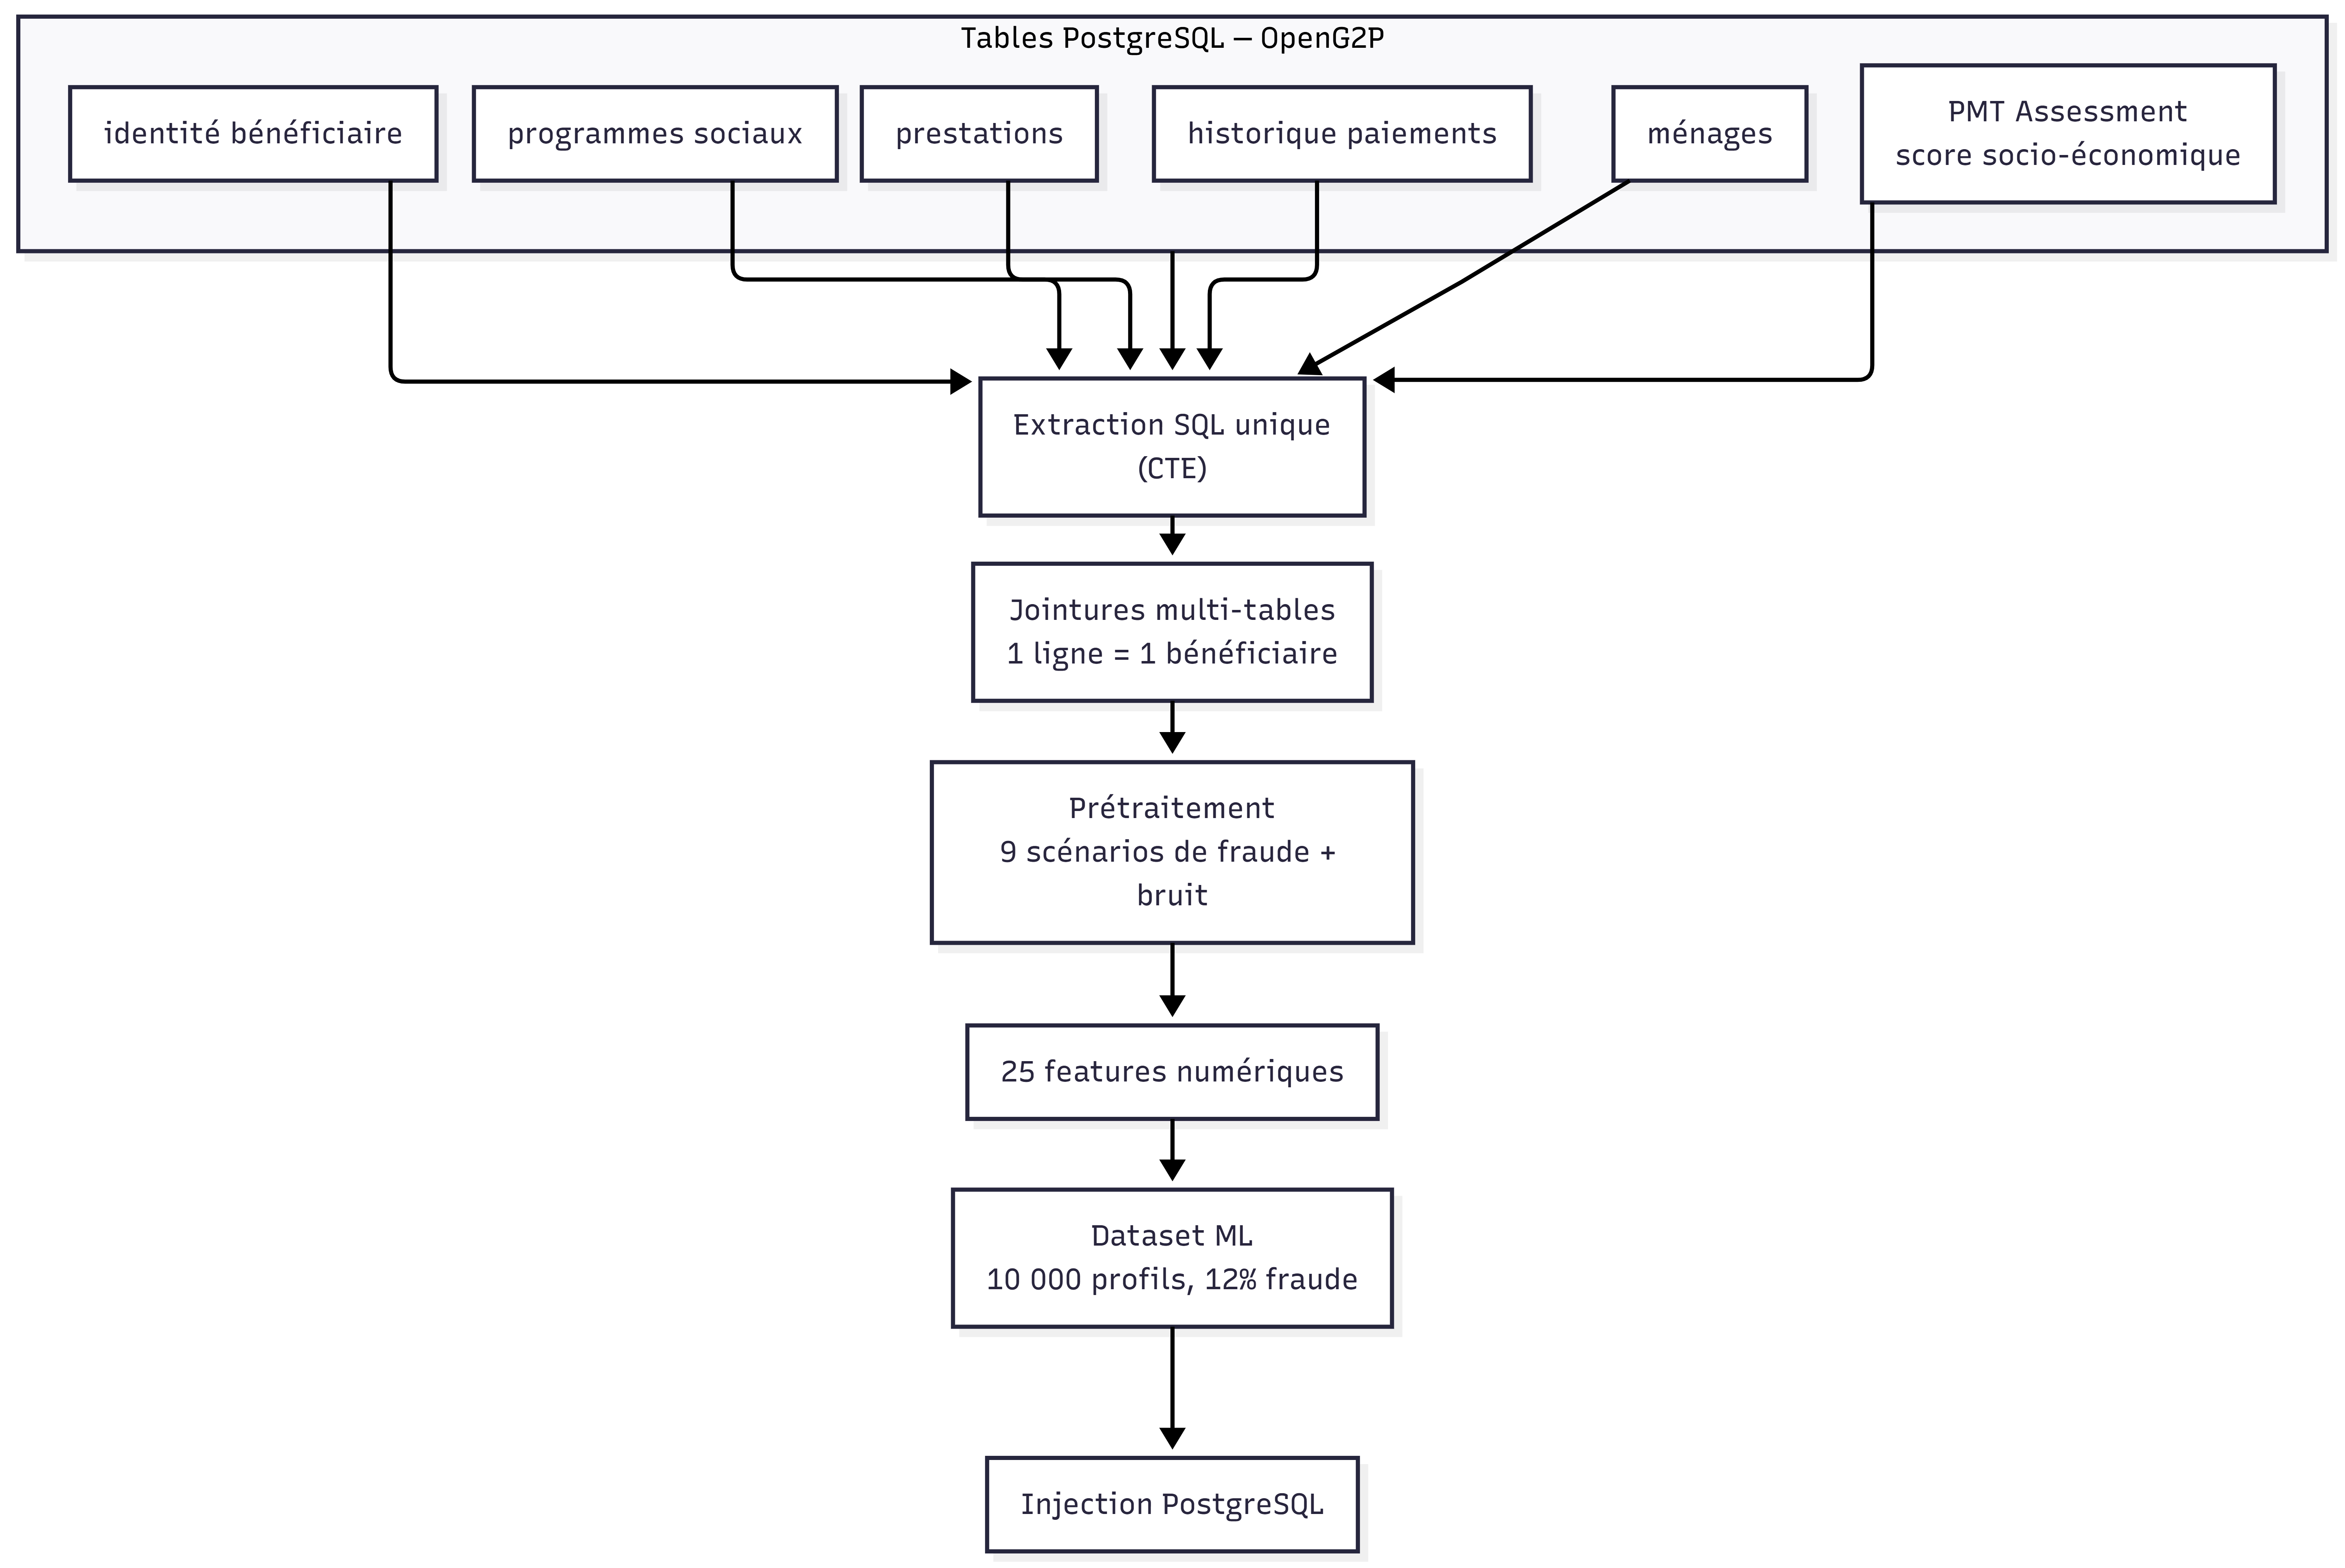
\includegraphics[width=0.7\textwidth]{DatasetGeneration.png}
    \caption{Processus de génération du dataset OpenG2P synthétique}
    \label{fig:generation-dataset}
\end{figure}


\hspace{0.5cm}L'objectif n'est pas uniquement de produire des données réalistes, mais également d'éviter que les profils frauduleux soient trop faciles à distinguer des profils légitimes. Si les deux classes étaient parfaitement séparées, les modèles obtiendraient d'excellents résultats pendant l'entraînement sans pour autant être capables de généraliser sur de nouveaux cas. C'est pourquoi un bruit contrôlé et des cas limites ont été introduits lors de la génération des données.

\hspace{0.5cm}La Figure~\ref{fig:pmt-score-dist} illustre cette approche à travers la distribution du score PMT. On observe un recouvrement important entre les bénéficiaires légitimes et frauduleux : les fraudes sont plus fréquentes pour les faibles valeurs de PMT, mais aucune frontière nette ne permet de les séparer. Cette distribution est volontairement recherchée afin de rapprocher le dataset des situations rencontrées en pratique.

\begin{figure}[H]
    \centering
    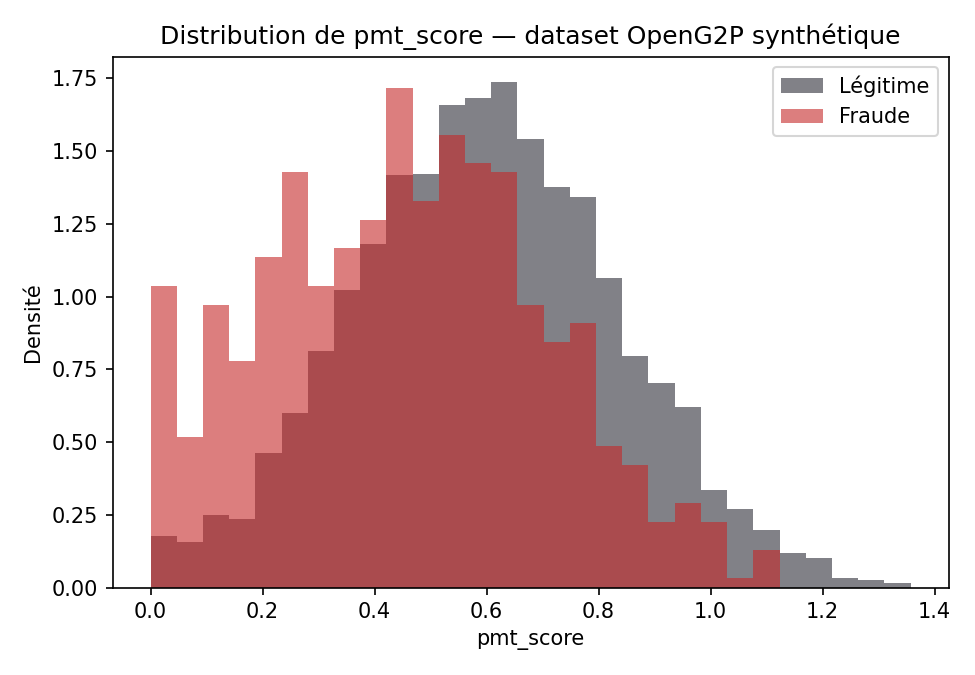
\includegraphics[width=0.7\textwidth]{openg2p_pmt_score_distribution.png}
    \caption{Distribution du score PMT selon la classe réelle dans le dataset OpenG2P synthétique}
    \label{fig:pmt-score-dist}
\end{figure}

\hspace{0.5cm}Le dataset obtenu constitue désormais la base de travail du moteur de détection de fraude. Les 28 features construites sont utilisées comme variables d'entrée par les différents modules du système : moteur de règles, modèles de Machine Learning, analyse de réseau et moteur d'explicabilité.

%---------------------------------------------------------------

\subsection{Un second banc d'essai : le dataset PaySim}
\label{sec:paysim}

\hspace{0.5cm}Bien que le dataset OpenG2P reproduise fidèlement le fonctionnement de la plateforme, il reste un jeu de données synthétique. Afin de vérifier que les modèles développés ne sont pas uniquement adaptés à ce contexte, un second jeu de données public, PaySim (Kaggle), a été utilisé lors de la phase d'entraînement et de validation.

\hspace{0.5cm}Contrairement à OpenG2P, où chaque ligne correspond à un bénéficiaire, PaySim contient des transactions de paiement mobile. Les variables décrivent notamment le montant de la transaction, les soldes des comptes avant et après l'opération ainsi que le type de transaction. Avant l'entraînement, une phase de préparation a été nécessaire : certaines colonnes présentaient une fuite de données en révélant directement les transactions frauduleuses. Ces variables ont donc été supprimées afin d'obtenir un jeu de données plus représentatif et d'éviter des performances artificiellement élevées.

\hspace{0.5cm}La Figure~\ref{fig:paysim-amount-dist} présente la distribution des montants des transactions après nettoyage. Comme pour le score PMT du dataset OpenG2P, les distributions des transactions légitimes et frauduleuses se chevauchent largement. Le montant seul ne permet donc pas d'identifier une fraude, ce qui confirme la nécessité de combiner plusieurs variables pour prendre une décision fiable.

\begin{figure}[H]
    \centering
    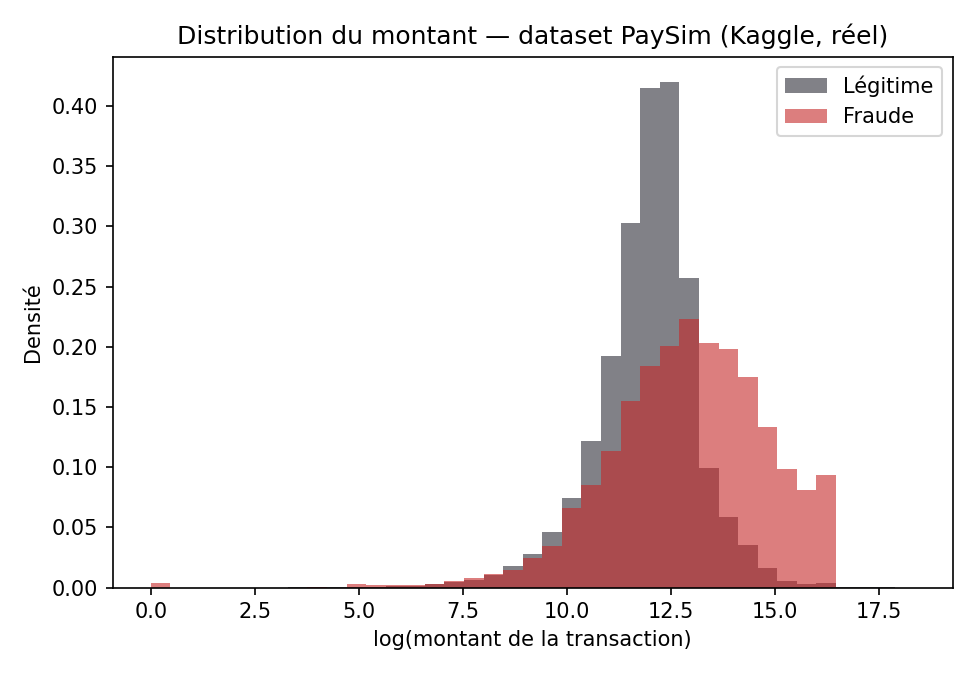
\includegraphics[width=0.7\textwidth]{paysim_amount_distribution.png}
    \caption{Distribution du montant des transactions selon la classe réelle dans le dataset PaySim}
    \label{fig:paysim-amount-dist}
\end{figure}

\hspace{0.5cm}Le modèle XGBoost entraîné sur les onze features retenues obtient d'excellentes performances (ROC-AUC de 1,000 et PR-AUC de 0,996). Ces résultats sont supérieurs à ceux obtenus sur OpenG2P, mais cette différence s'explique principalement par la nature des données. Les fraudes bancaires présentes dans PaySim laissent des indices plus marqués, tandis que les fraudes liées aux bénéficiaires d'aides sociales sont généralement plus discrètes et réparties sur plusieurs dimensions, comme le revenu, les relations entre bénéficiaires ou l'historique des paiements.

\hspace{0.5cm}L'utilisation de PaySim a apporté plusieurs bénéfices. Elle a d'abord permis d'identifier et de corriger des fuites de données, puis de valider l'utilisation de métriques adaptées aux jeux de données déséquilibrés, comme le PR-AUC. Enfin, elle a confirmé que le pipeline d'entraînement développé n'est pas spécifique au seul dataset OpenG2P et reste performant sur un contexte totalement différent.

\hspace{0.5cm}PaySim n'a toutefois pas vocation à remplacer le dataset OpenG2P. Il est uniquement utilisé comme jeu de validation complémentaire. Son rôle est de démontrer que les méthodes et les modèles retenus restent efficaces sur des données réelles, tout en conservant OpenG2P comme base principale du moteur de détection de fraude.
\subsection{Moteur de détection de fraude}

\hspace{0.5cm}Avant même de faire appel à l'apprentissage automatique, le système applique une première ligne de détection~: le moteur de règles. Il permet de capter des patterns de fraude connus sans avoir besoin d'un modèle ML — une approche déterministe et immédiatement interprétable, qui complète les modèles statistiques développés dans la suite du chapitre. Chaque règle est définie sous la forme d'une condition, d'un poids et d'un niveau de sévérité.

\hspace{0.5cm}Les dix règles couvrent les scénarios suivants~: partage de compte bancaire (poids 0,35), partage de téléphone (poids 0,30), trop de programmes (poids 0,30), score PMT suspect (poids 0,20), écart de paiements (poids 0,30), ménage fantôme (poids 0,25), combinaison téléphone et compte (poids 0,40), risque réseau élevé (poids 0,30), sous-déclaration de revenus (poids 0,20), et manipulation combinée au réseau (poids 0,35).

\hspace{0.5cm}Les conditions de ces règles sont évaluées de façon sécurisée, sans jamais exécuter de code arbitraire — un choix d'implémentation déterminant puisque les règles peuvent, à terme, être modifiées par un administrateur métier sans revalidation du code source.

\hspace{0.5cm}Le score de règles correspond à la somme des poids des règles déclenchées, plafonnée à 1. Une liste de signaux (par exemple compte partagé, ou combinaison réseau frauduleux) accompagne ce score pour expliquer les déclenchements.

\hspace{0.5cm}Si le moteur de règles capture efficacement les patterns de fraude déjà répertoriés, il reste par nature limité aux scénarios anticipés lors de sa conception. La détection de patterns plus subtils ou non explicitement codifiés nécessite un second moteur, statistique cette fois~: le pipeline de Machine Learning.

\subsection{Conception du moteur de détection de fraude par Machine Learning}

\hspace{0.5cm}Le pipeline de Machine Learning ne repose pas sur un modèle unique, mais sur un \textbf{ensemble à deux étages} (\textit{stacking})~: trois modèles supervisés de nature différente sont d'abord entraînés indépendamment sur les mêmes 28 features, puis un méta-modèle apprend à combiner leurs trois prédictions en un score unique, plus fiable que n'importe lequel des trois pris isolément. Un quatrième modèle, non supervisé, complète cet ensemble pour couvrir les fraudes qu'aucun exemple d'entraînement ne représente encore.

\hspace{0.5cm}Le dataset utilisé pour l'entraînement est déséquilibré~: comme le montre la Figure~\ref{fig:class-balance}, seuls 13,2~\% des bénéficiaires du jeu d'entraînement sont étiquetés comme frauduleux. Sans traitement, ce déséquilibre biaiserait tout modèle supervisé vers la classe majoritaire, au risque de manquer une part importante des vraies fraudes. Plutôt que de générer des exemples synthétiques de la classe minoritaire, la correction retenue agit directement sur la fonction de coût de chaque modèle~: Random Forest et Régression Logistique pénalisent davantage une erreur sur la classe fraude via \texttt{class\_weight="balanced"}, et XGBoost applique un facteur \texttt{scale\_pos\_weight} qui amplifie le gradient des exemples frauduleux mal classés. Cette approche a l'avantage de ne jamais introduire de données artificielles dans l'entraînement~: chaque exemple vu par les modèles est un profil réellement généré, seule l'importance qui lui est accordée pendant l'apprentissage varie.

\begin{figure}[H]
    \centering
    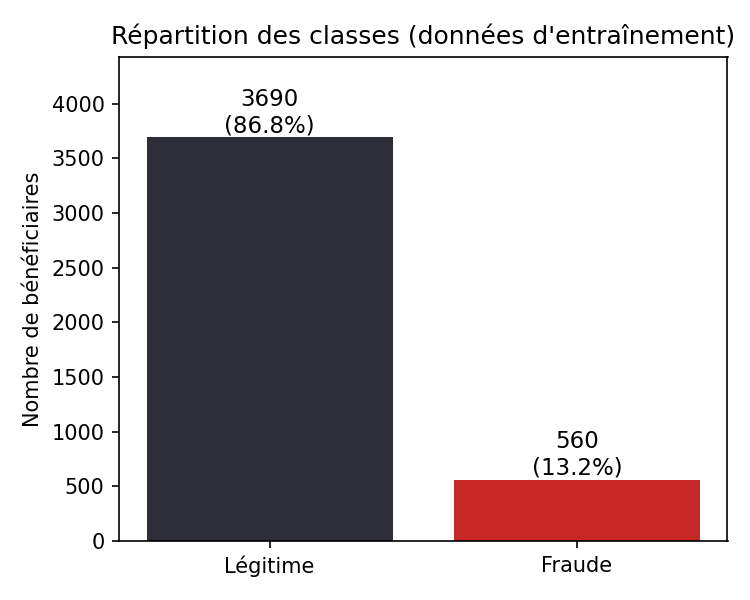
\includegraphics[width=0.55\textwidth]{class_balance.png}
    \caption{Répartition des classes dans les données d'entraînement}
    \label{fig:class-balance}
\end{figure}

\hspace{0.5cm}Les trois modèles de base sont évalués individuellement sur un jeu de test (\textit{holdout}) de 750 bénéficiaires jamais vus à l'entraînement, avant que leurs prédictions ne soient combinées. Le Tableau~\ref{tab:comparaison_modeles} compare leurs performances respectives à celles de l'ensemble final, et la Figure~\ref{fig:roc-comparaison} illustre leurs courbes ROC.

\begin{table}[H]
\centering
\caption{Comparaison des modèles de base et de l'ensemble (jeu de test, seuil 0,5)}
\label{tab:comparaison_modeles}
\renewcommand{\arraystretch}{1.4}
\begin{tabular}{lcccc}
\hline
\thead{Modèle} & \thead{AUC-ROC} & \thead{F1 (fraude)} & \thead{Précision} & \thead{Rappel} \\
\hline
Random Forest & 0.905 & 0.704 & 0.933 & 0.566 \\
\rowcolor{EYgray}
XGBoost & 0.913 & 0.807 & 0.890 & 0.737 \\
Régression Logistique & 0.874 & 0.561 & 0.448 & 0.747 \\
\hline
\rowcolor{EYyellow!30}
\textbf{Ensemble (stacking, retenu)} & \textbf{0.912} & \textbf{0.721} & \textbf{0.658} & \textbf{0.798} \\
\hline
\end{tabular}
\end{table}

\begin{figure}[H]
    \centering
    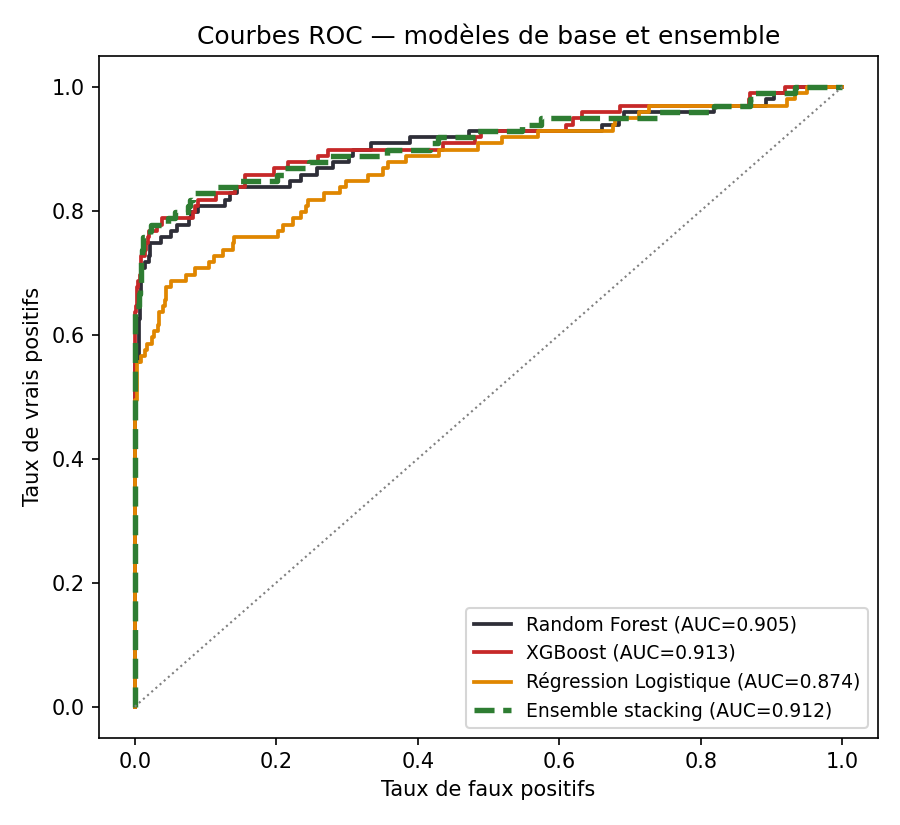
\includegraphics[width=0.8\textwidth]{roc_comparaison_modeles.png}
    \caption{Courbes ROC comparées des trois modèles de base et de l'ensemble}
    \label{fig:roc-comparaison}
\end{figure}

\hspace{0.5cm}Aucun des trois modèles de base ne domine les autres sur tous les critères~: XGBoost obtient le meilleur F1 et le meilleur rappel pris isolément, Random Forest la meilleure précision, et la Régression Logistique — bien que la plus faible en AUC — un rappel proche de celui de XGBoost. C'est précisément cette complémentarité que le méta-modèle exploite~: en apprenant le poids à accorder à chacun plutôt qu'en imposant une combinaison fixe, l'ensemble atteint un rappel de 0,798, supérieur à celui de chacun des trois modèles pris seul, tout en conservant un AUC proche du meilleur modèle individuel. Un ajustement du seuil de décision (0,55 au lieu de 0,5, retrouvé par recherche sur les prédictions hors-échantillon de la validation croisée) porte le F1 final à 0,748.

\hspace{0.5cm}En complément de ces trois modèles supervisés, un modèle \textbf{Isolation Forest} détecte les bénéficiaires dont le comportement est statistiquement atypique, sans avoir besoin d'exemples de fraude étiquetés~: il isole chaque profil en le séparant aléatoirement des autres, les profils anormaux nécessitant nettement moins d'étapes de séparation que les profils courants. La Figure~\ref{fig:isolation-forest} compare la distribution de ce score d'anomalie entre bénéficiaires légitimes et frauduleux~: les fraudeurs se concentrent nettement vers les scores les plus élevés, même si un recouvrement subsiste dans la zone intermédiaire — ce chevauchement partiel est attendu, un modèle non supervisé n'ayant par construction aucune connaissance du label réel.

\begin{figure}[H]
    \centering
    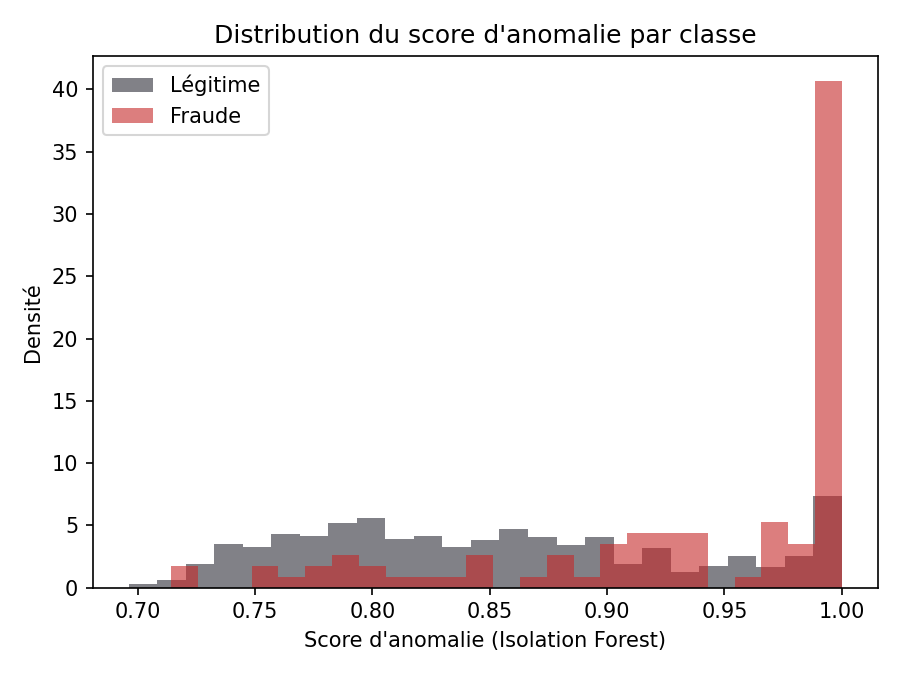
\includegraphics[width=0.7\textwidth]{isolation_forest_distribution.png}
    \caption{Distribution du score d'anomalie (Isolation Forest) par classe réelle}
    \label{fig:isolation-forest}
\end{figure}

\hspace{0.5cm}Ce filet de sécurité non supervisé est calculé pour chaque bénéficiaire et exposé dans l'API du moteur, où il enrichit le contexte d'explicabilité~; son intégration au score pondéré final est discutée dans la sous-section~\ref{sec:score-hybride}.

\hspace{0.5cm}Le moteur ML détecte efficacement les anomalies au niveau individuel, mais certaines fraudes ne se révèlent qu'au niveau collectif — lorsque plusieurs bénéficiaires partagent des ressources entre eux. C'est ce que l'analyse de réseau vient compléter.

\subsection{Analyse de réseau}

\hspace{0.5cm}Les fraudes organisées, comme le partage de compte bancaire entre plusieurs bénéficiaires fictifs, ne sont pas toujours visibles au niveau individuel. L'analyse de réseau les révèle en construisant un graphe où les nœuds sont les bénéficiaires et les arêtes représentent des ressources partagées. La Figure~\ref{fig:network-pipeline} résume l'ensemble de ce traitement, depuis les données brutes d'OpenG2P jusqu'à la contribution du score réseau au score hybride final.

\begin{figure}[H]
    \centering
    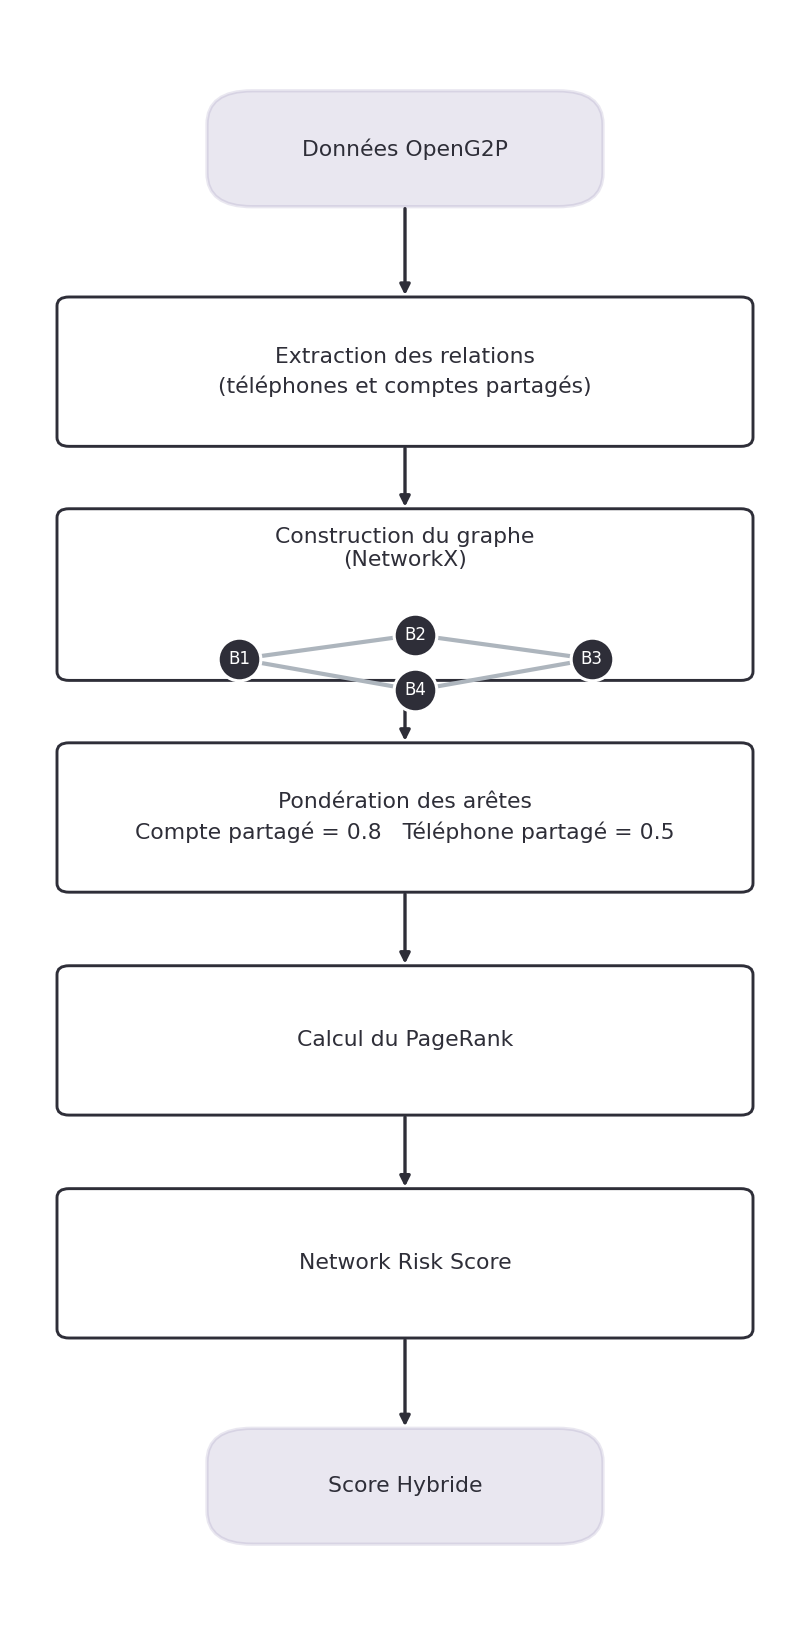
\includegraphics[width=0.45\textwidth]{network_analysis_pipeline.png}
    \caption{Pipeline de l'analyse de réseau~: extraction des relations, construction du graphe, pondération des arêtes et calcul du PageRank}
    \label{fig:network-pipeline}
\end{figure}

\hspace{0.5cm}Les comptes bancaires partagés se voient attribuer un poids double par rapport aux téléphones partagés (0,8 contre 0,5), car ils représentent un signal de fraude plus fort~: partager un numéro de téléphone peut être légitime en contexte rural, mais partager un compte bancaire est très rarement justifiable. L'algorithme PageRank est ensuite appliqué sur ce graphe pour identifier les nœuds les plus centraux, donc les plus susceptibles d'appartenir à un réseau frauduleux organisé.

\hspace{0.5cm}À ce stade, le système dispose de trois signaux indépendants — règles, ML, réseau — chacun capturant une facette différente du risque de fraude. Encore faut-il les combiner en une décision unique et exploitable~: c'est le rôle de la fusion des scores.

\subsection{Fusion des scores}
\label{sec:score-hybride}

\hspace{0.5cm}Le moteur de détection combine trois sources d'information complémentaires : le moteur de règles, le modèle de Machine Learning et l'analyse de réseau. Cette approche s'inspire du principe du \textit{stacking}, qui consiste à fusionner plusieurs prédictions afin d'améliorer la qualité de la décision finale \cite{Nocairi2016}. De manière générale, cette combinaison est exprimée par :

\begin{equation}
\hat{y} = \sum_{m=1}^{M} w_m f_m(x)
\label{eq:model-averaging}
\end{equation}

\hspace{0.5cm}où $f_m(x)$ représente la prédiction du modèle $m$ et $w_m$ son poids dans la décision finale. Dans notre système, cette formule est adaptée pour combiner les trois scores produits par les différents modules :

\begin{equation}
\text{score\_final}=0{,}55 \times s_{\text{ML}}
+0{,}20 \times s_{\text{règles}}
+0{,}25 \times s_{\text{graphe}}
\label{eq:score-hybride}
\end{equation}

\hspace{0.5cm}\textbf{Le modèle de Machine Learning reçoit le poids le plus élevé (55\,\%),} car il apprend automatiquement des relations complexes à partir des données. Le moteur de règles (20\,\%) apporte une détection simple et facilement interprétable des scénarios connus, tandis que l'analyse de réseau (25\,\%) permet d'identifier les fraudes organisées entre plusieurs bénéficiaires.

\hspace{0.5cm}Ces poids ont été définis lors de la conception du système afin d'exploiter les points forts de chaque approche. Contrairement à l'étude de Noçairi et al., où les poids sont appris automatiquement à partir des données, ils sont ici fixés manuellement. L'apprentissage automatique de ces poids constitue une perspective d'amélioration.

\hspace{0.5cm}Le score obtenu est ensuite converti en quatre niveaux de risque \textbf{(LOW, MEDIUM, HIGH et CRITICAL)}, ce qui facilite la priorisation des dossiers à examiner.

\hspace{0.5cm}Le score d'anomalie fourni par l'Isolation Forest est également calculé, mais il n'est pas encore intégré à cette formule. Il est actuellement utilisé comme un indicateur complémentaire pour l'explicabilité et le suivi des résultats.

\hspace{0.5cm}Une fois le score de risque calculé, il reste à expliquer les raisons qui ont conduit à cette décision. Les deux modules suivants, SHAP et le modèle de langage Mistral, répondent à cet objectif en fournissant une explication claire des résultats.

\subsection{Explicabilité SHAP}

\hspace{0.5cm}Un score seul n'est pas exploitable par un agent social~: encore faut-il pouvoir justifier pourquoi un bénéficiaire donné a été signalé. Le moteur intelligent génère deux niveaux d'explication, dont le premier repose sur SHAP.

\hspace{0.5cm}SHAP (\textit{SHapley Additive exPlanations}) décompose la prédiction du modèle XGBoost en contributions individuelles de chaque feature, ce qui permet d'identifier les variables ayant le plus influencé le score attribué à un bénéficiaire donné. La Figure~\ref{fig:shap} illustre cette répartition de l'importance des variables sur l'ensemble des prédictions du jeu de test~: chaque point représente un bénéficiaire, sa position horizontale son impact sur le score (positif ou négatif), et sa couleur la valeur de la feature pour ce bénéficiaire (rouge~: valeur élevée, bleu~: valeur faible).

\begin{figure}[H]
    \centering
    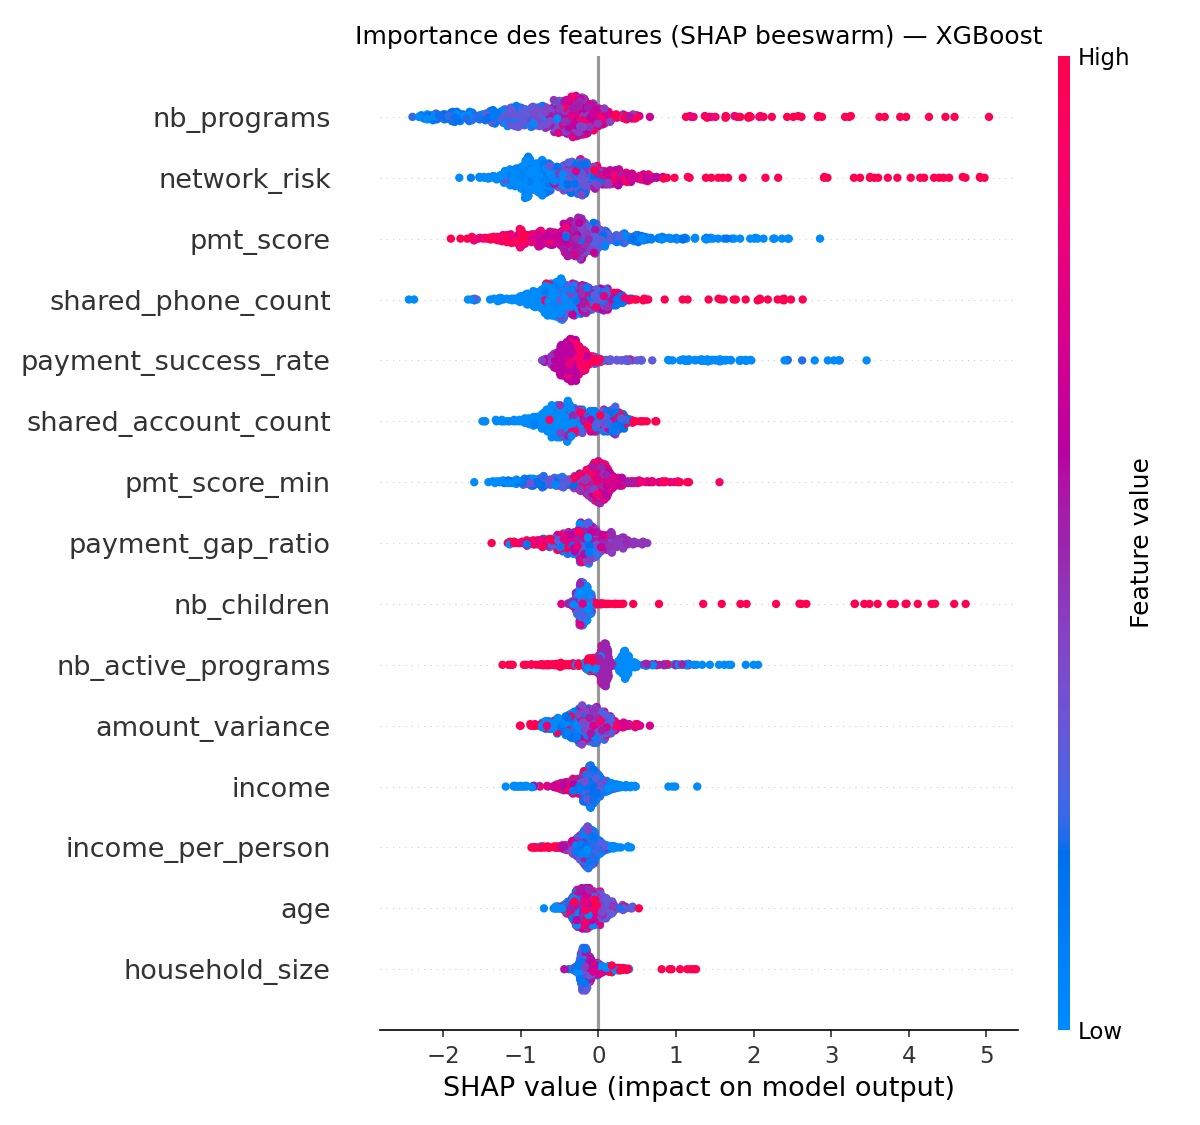
\includegraphics[width=0.85\textwidth]{shap_beeswarm.png}
    \caption{Importance globale des features (SHAP beeswarm) sur le jeu de test}
    \label{fig:shap}
\end{figure}

\hspace{0.5cm}Le modèle XGBoost accorde principalement de l'importance au nombre de programmes, au risque du réseau et aux indicateurs de paiement. Les variables liées au partage de téléphone ou de compte contribuent également à la détection de comportements potentiellement frauduleux. À l'inverse, certaines caractéristiques socio-économiques telles que le revenu et l'âge ont une influence plus limitée.

\hspace{0.5cm}On observe par exemple qu'un \texttt{nb\_programs} élevé (points rouges à droite) pousse systématiquement le score vers la fraude, alors qu'un \texttt{pmt\_score} élevé (points bleus à droite, rouges à gauche) le pousse plutôt vers un profil légitime — cohérent avec l'intuition métier~: un score PMT élevé signale un ménage moins vulnérable, donc moins susceptible de frauder pour capter une aide.

\begin{figure}[H]
    \centering
    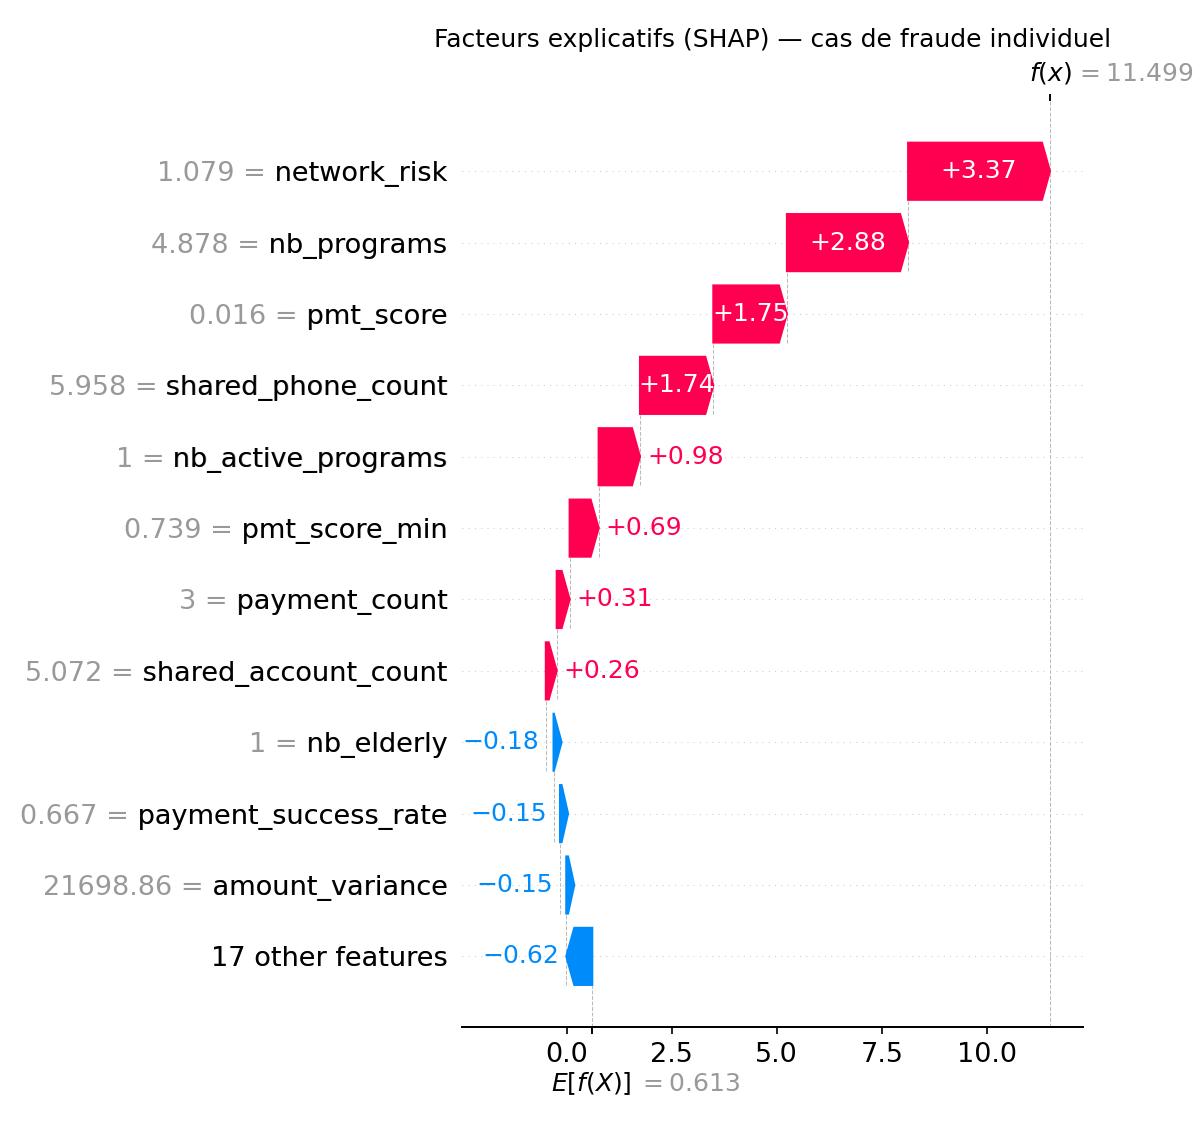
\includegraphics[width=0.75\textwidth]{shap_waterfall.png}
    \caption{Facteurs explicatifs SHAP pour un cas de fraude individuel}
    \label{fig:shap-waterfall}
\end{figure}

\hspace{0.5cm}Cette décomposition technique, bien qu'indispensable pour un data scientist ou un auditeur, demeure difficile à interpréter directement par un agent social non spécialiste. La dernière couche du pipeline traduit donc ces facteurs SHAP en une explication rédigée en langage naturel.

\subsection{Explication LLM}

\hspace{0.5cm}Le modèle de langage Mistral reçoit les facteurs SHAP, le score final et les signaux déclenchés, puis génère une explication lisible. Le module RAG (ChromaDB) enrichit ce contexte avec des cas de fraude similaires issus de la base de connaissance, ce qui permet à l'explication générée de s'appuyer sur des précédents comparables plutôt que sur les seules variables numériques.

\hspace{0.5cm}\textbf{Exemple de réponse générée~:} La Figure~\ref{fig:explication-llm} vous montre un exemple d'explication générée pour un bénéficiaire réel du jeu de test. L'agent social peut ainsi comprendre immédiatement les raisons du signalement et décider d'une action appropriée.
\begin{quote}
\textit{«~Getachew Daniel partage son compte bancaire avec Thomas Agyeman, un autre bénéficiaire du même programme. Il est également inscrit dans plusieurs autres programmes en même temps, ce qui constitue un risque très élevé.»}
\end{quote}
\begin{figure}[H]
    \centering
    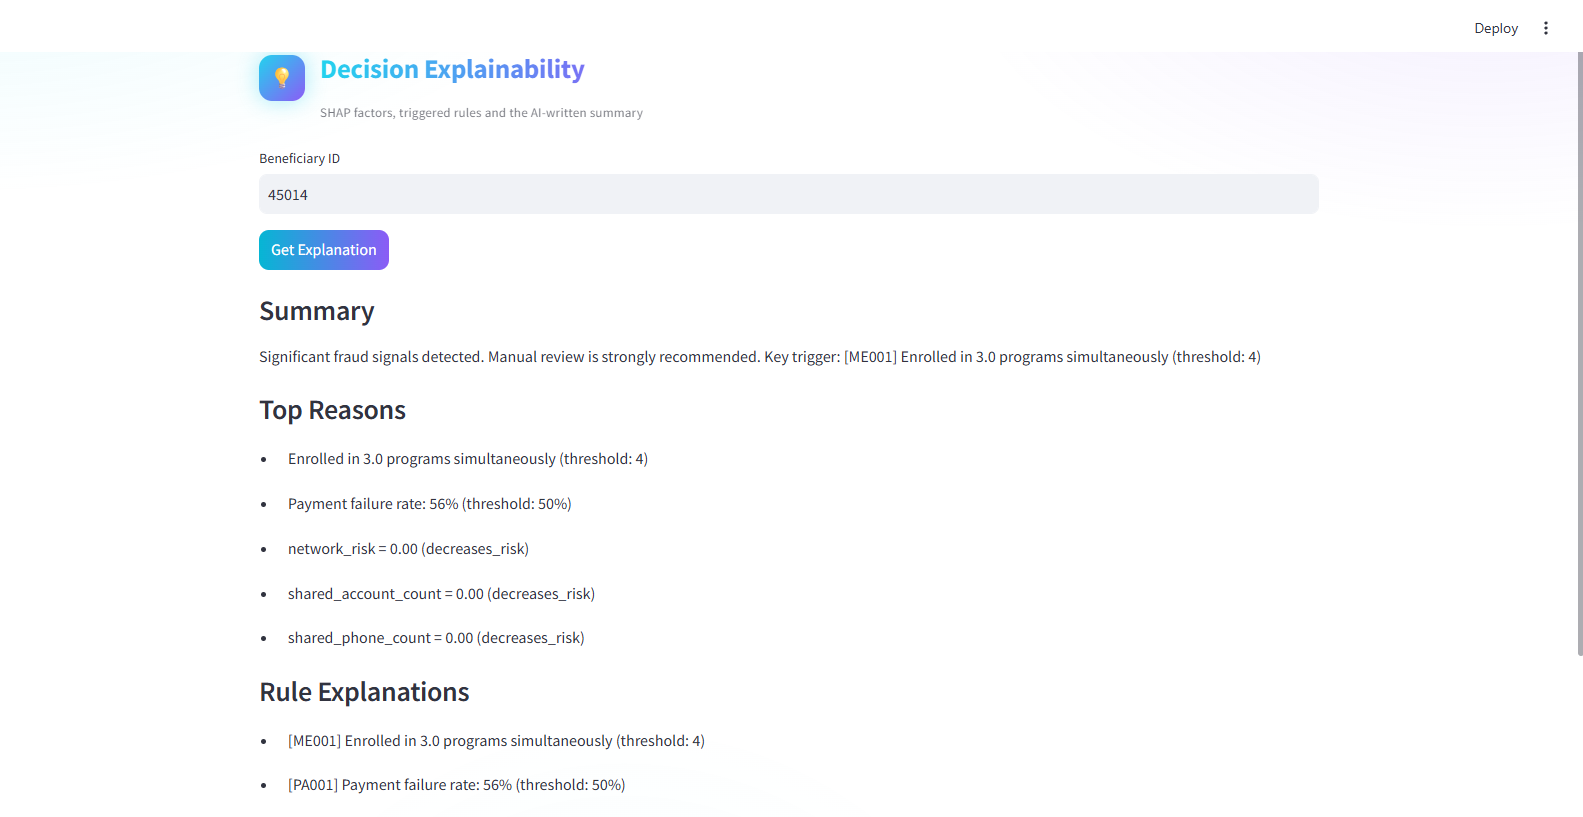
\includegraphics[width=\textwidth]{explainability.png}
    \caption{Explication LLM détaillée générée pour un bénéficiaire intégrée dans le tableau de bord}
    \label{fig:explication-llm}
\end{figure}

\begin{figure}[H]
    \centering
    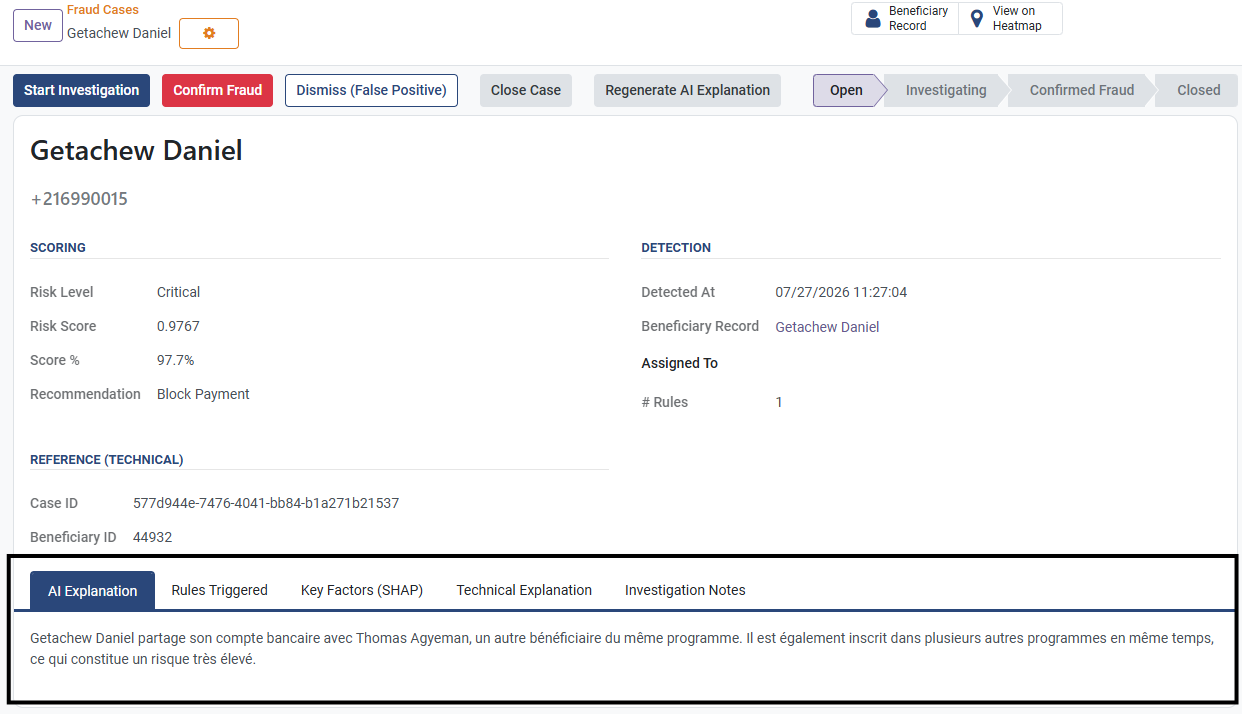
\includegraphics[width=\textwidth]{explainability2.png}
    \caption{Explication LLM simple générée pour un bénéficiaire intégrée dans le tableau de bord}
    \label{fig:explication-llm-2}
\end{figure}


\hspace{0.5cm}Avec cette explication en langage naturel, le pipeline de scoring est complet~: de l'extraction des données jusqu'à la restitution d'une décision justifiée. Reste à situer ce pipeline dans son environnement d'exploitation réel — comment il est exposé, synchronisé avec Odoo, restitué dans un tableau de bord, et déployé en production. C'est l'objet de la section suivante.

% ─────────────────────────────────────────────────────────────
\section{Intégration dans OpenG2P}
% ─────────────────────────────────────────────────────────────

\hspace{0.5cm}Le moteur intelligent, aussi complet soit-il, n'a de valeur opérationnelle que s'il s'intègre naturellement dans le quotidien des agents sociaux qui utilisent OpenG2P. Cette section décrit les quatre mécanismes qui assurent cette intégration~: l'exposition du pipeline sous forme de service, la synchronisation automatique avec Odoo, la restitution visuelle dans le tableau de bord, et le déploiement d'ensemble via Docker.

\subsection{Synchronisation Odoo}

\hspace{0.5cm}Un module Odoo personnalisé synchronise périodiquement les cas de fraude détectés par le moteur intelligent et les affiche dans un menu dédié, sans quitter l'interface OpenG2P.

\hspace{0.5cm}Un mécanisme de notification automatique permet également de déclencher un scoring en tâche de fond dès qu'un bénéficiaire est créé ou mis à jour dans OpenG2P, sans action manuelle de l'agent. Cette synchronisation garantit que la donnée reste fraîche côté Odoo sans imposer à l'agent social un aller-retour vers un outil distinct.

\begin{figure}[H]
    \centering
    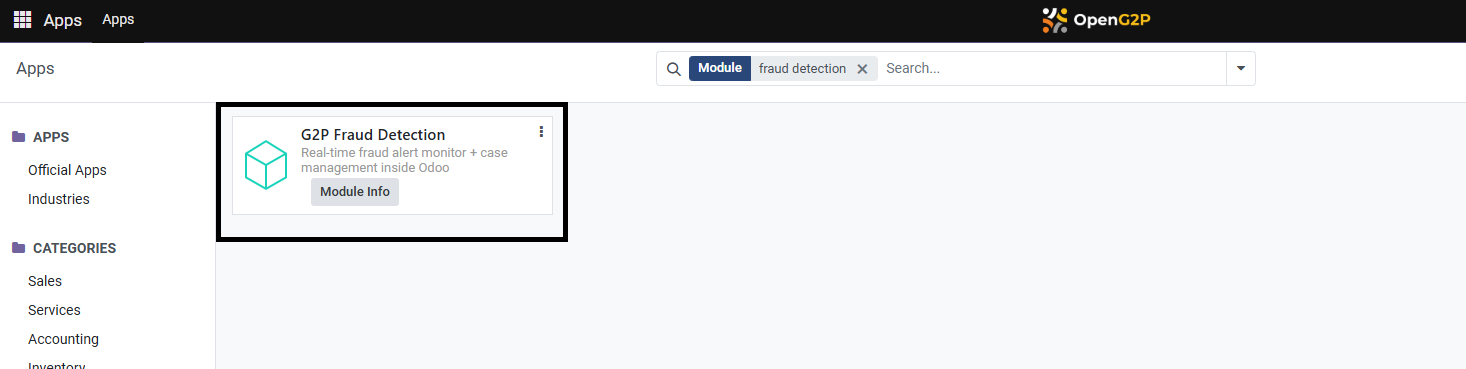
\includegraphics[width=0.72\textwidth]{IntegrationOdoo.png}
    \caption{Intégration du module de détection de fraude dans Odoo}
    \label{fig:integration-odoo}
\end{figure}

\hspace{0.5cm}La Figure~\ref{fig:integration-odoo} illustre l'intégration du module de détection de fraude dans Odoo. 

\vspace{0.3cm}
{\large \textbf{Générateur de notification intégré a Odoo }}
\vspace{0.2cm}
\begin{figure}[H]
    \centering
    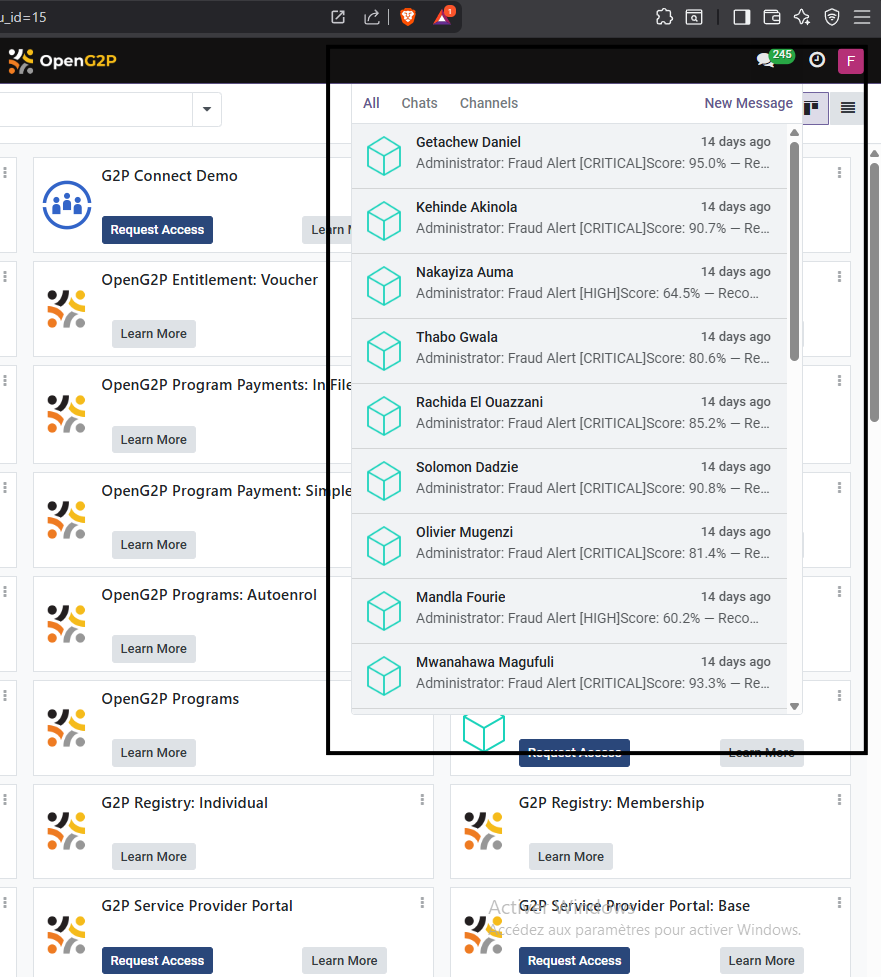
\includegraphics[width=0.42\textwidth]{notifications.png}
    \caption{Intégration du module de notification d'alertes synchronisées dans Odoo}
    \label{fig:notification-odoo}
\end{figure}
\hspace{0.5cm}La Figure~\ref{fig:notification-odoo} montre le module de notification d'alertes synchronisées dans Odoo, qui permet aux agents sociaux de recevoir des alertes en temps réel sur les bénéficiaires à risque.
\begin{figure}[H]
    \centering
    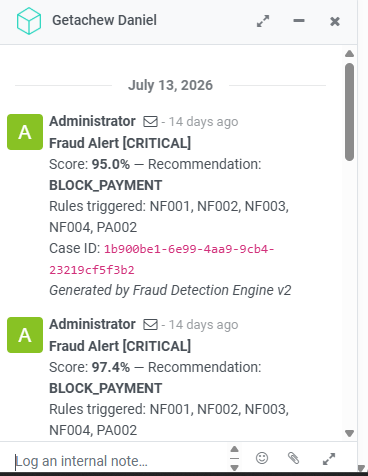
\includegraphics[width=0.5\textwidth]{notifications2.png}
    \caption{Intégration du module de notification: détails d'une alerte Odoo}
    \label{fig:notification-odoo2}
\end{figure}

\hspace{0.5cm}La Figure~\ref{fig:notification-odoo2} montre les détails d'une alerte synchronisée dans Odoo comme le bénéficiaire concerné, le score de risque et les signaux déclenchés. L'agent social peut ainsi prendre connaissance de l'alerte et décider des actions à entreprendre directement depuis l'interface Odoo.
\newline
\vspace{0.3cm}
{\large \textbf{Vue kanban des cas de fraude}}
\vspace{0.2cm}

\begin{figure}[H]
    \centering
    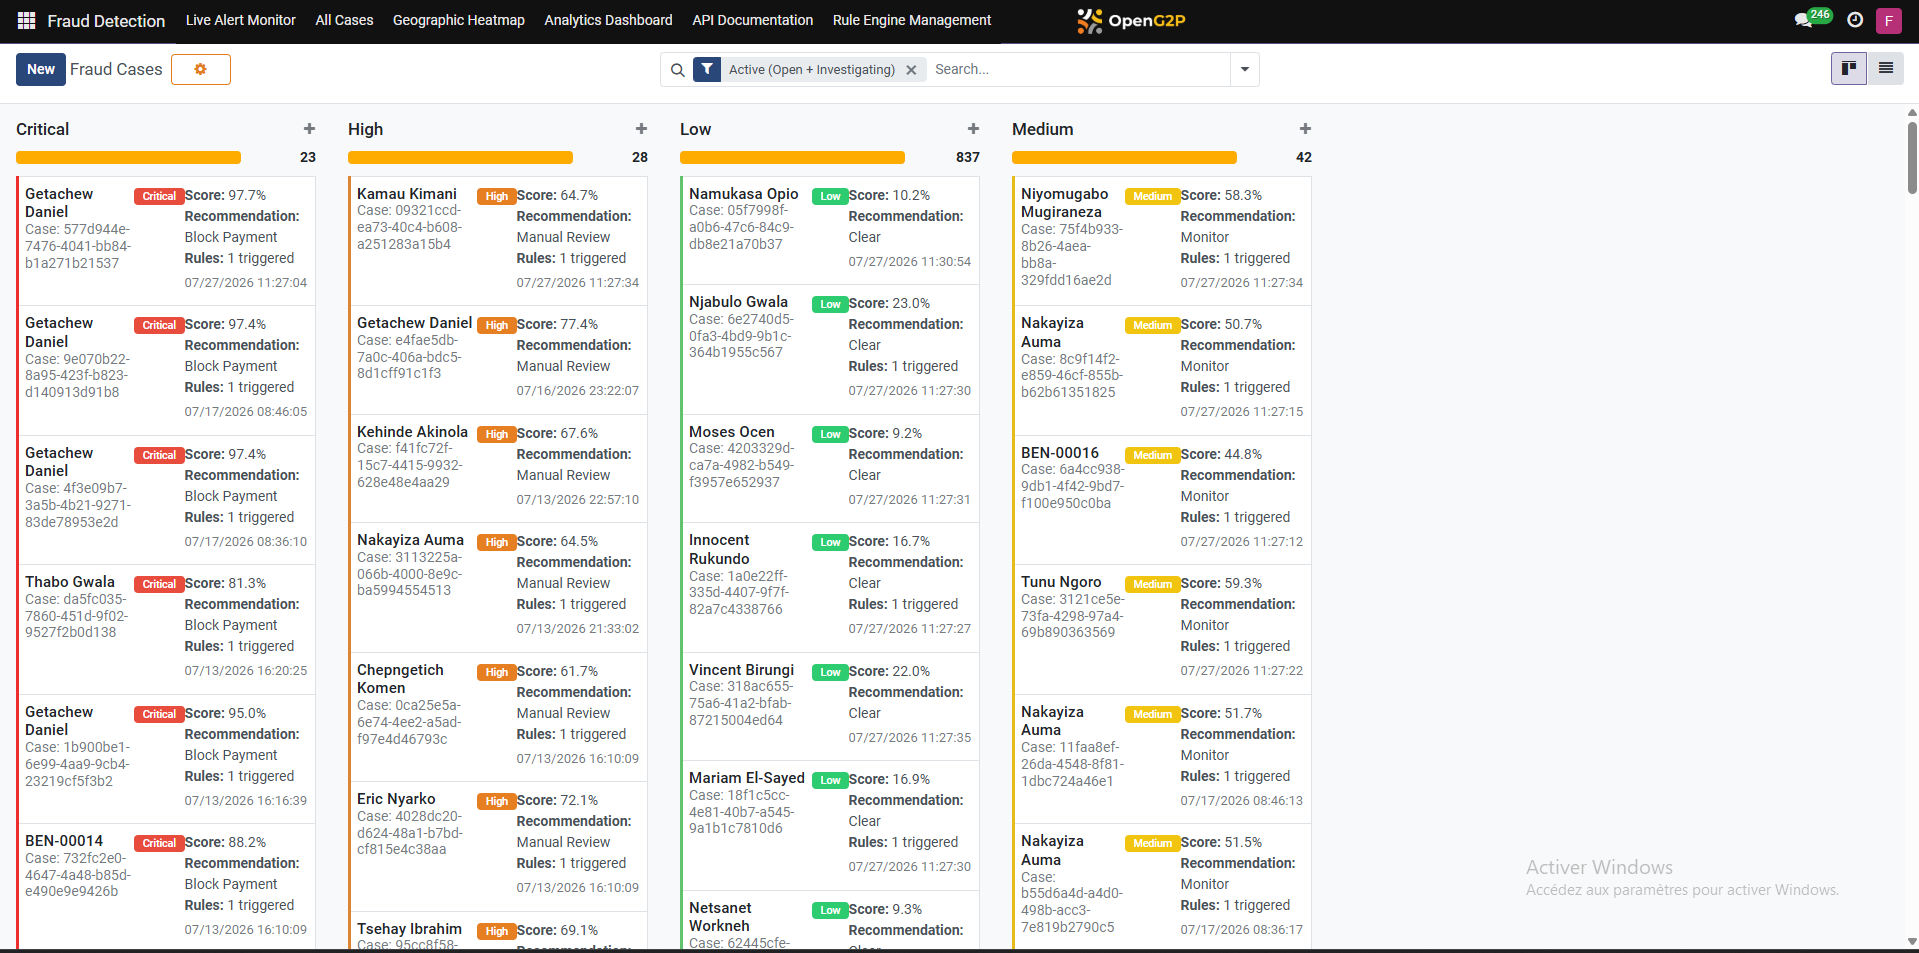
\includegraphics[width=\textwidth]{fraudcase.png}
    \caption{Tableau de bord: vue des alertes actives avec niveaux de risque intégré dans Odoo}
    \label{fig:dashboard-alertes}
\end{figure}
\hspace{0.5cm}La Figure~\ref{fig:dashboard-alertes} montre le tableau de bord intégré dans Odoo, qui permet aux agents sociaux de visualiser les alertes actives avec les niveaux de risque associés. Les agents peuvent filtrer les alertes par programme, niveau de risque et date, et accéder aux détails de chaque cas pour prendre des décisions éclairées.

\vspace{0.3cm}
{\large \textbf{Suivi des alertes en temps réel }}
\vspace{0.2cm}
\begin{figure}[H]
    \centering
    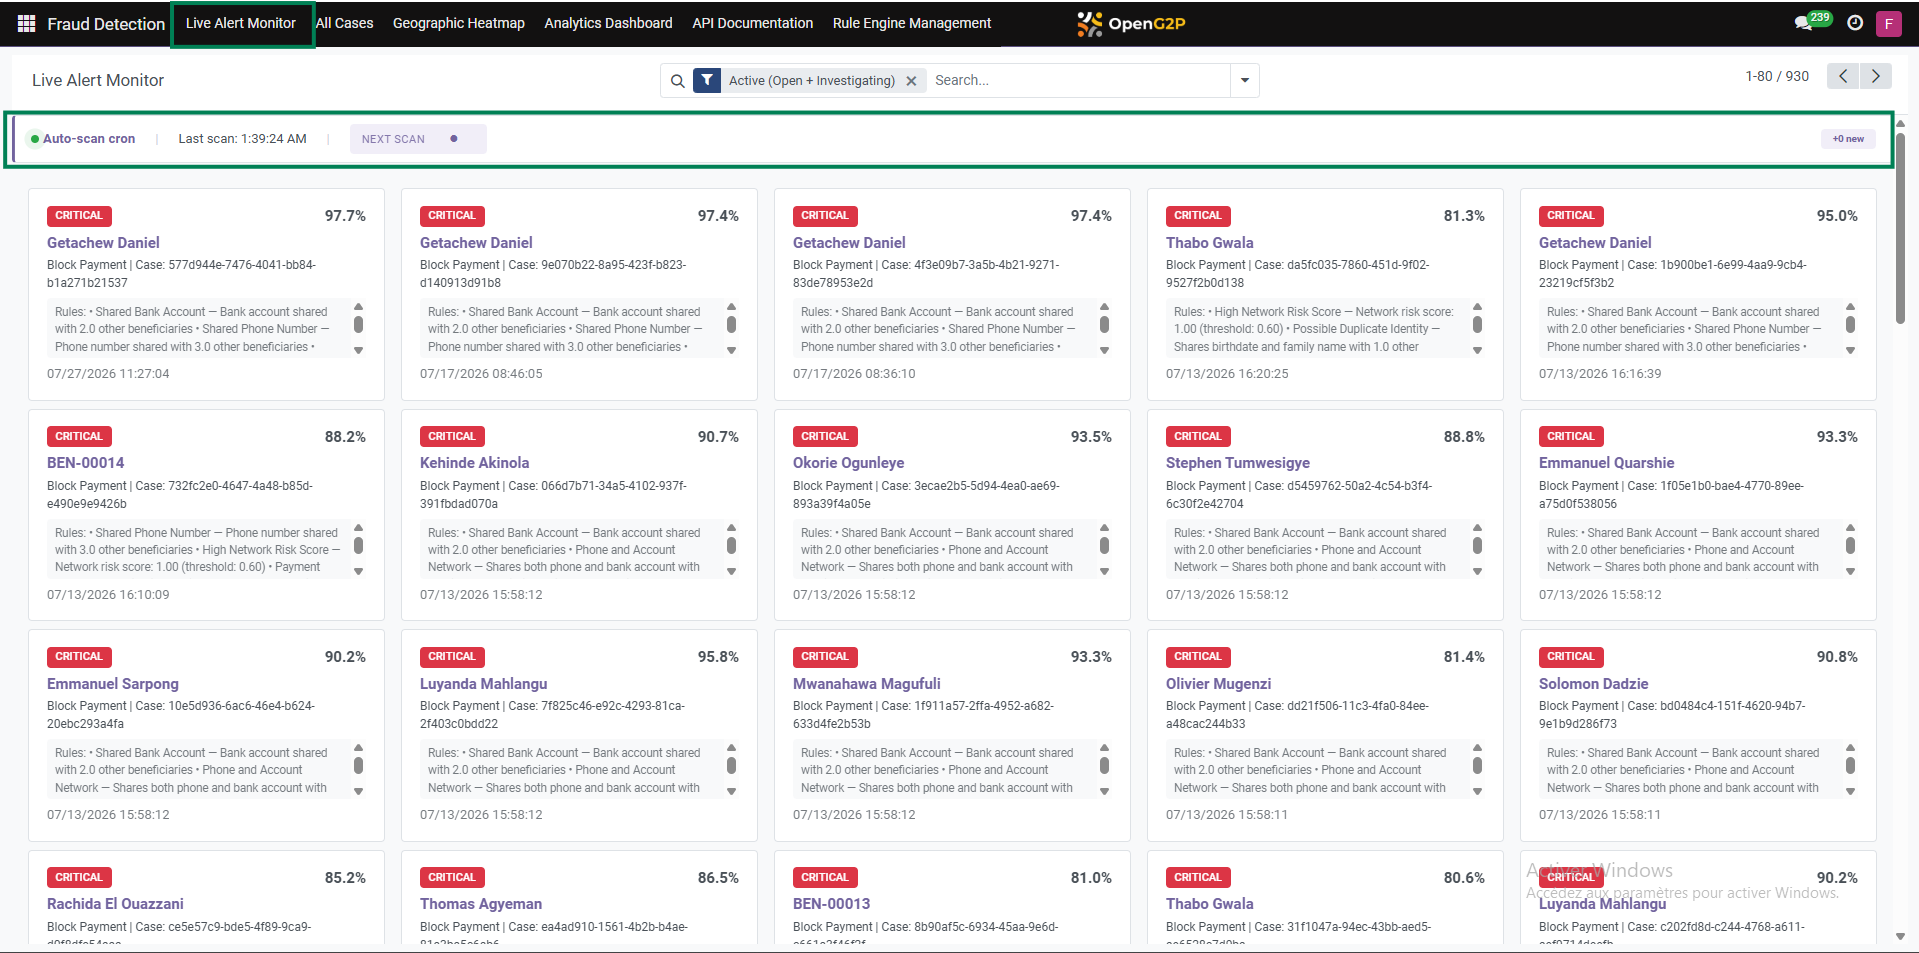
\includegraphics[width=\textwidth]{LiveAlertMonitor.png}
    \caption{Tableau de bord Odoo: vue du scanner en temps-réel de la base de données  }
    \label{fig:live-alert-Monitor}
\end{figure}
\hspace{0.5cm}La Figure~\ref{fig:live-alert-Monitor} montre le tableau de bord du scanner en temps réel de la base de données, qui permet aux analystes fraude de suivre l'évolution des alertes et des cas de fraude détectés par le moteur intelligent. Les agents peuvent visualiser les tendances, les statistiques et les indicateurs clés pour prendre des décisions stratégiques.

\vspace{0.3cm}
{\large \textbf{Traitement d'un cas dans Odoo}}
\vspace{0.2cm}

\hspace{0.5cm}Une fois synchronisé dans OpenG2P, chaque cas de fraude s'ouvre dans une fiche dédiée (Figure~\ref{fig:odoo-case}) rassemblant toutes les informations nécessaires à la décision~: identité et contact du bénéficiaire, niveau de risque, score et recommandation du moteur, ainsi que le nombre de règles déclenchées.

\hspace{0.5cm}L'analyste dispose de quatre actions directement accessibles depuis cette fiche~: \textbf{démarrer une investigation}, \textbf{confirmer la fraude}, \textbf{rejeter comme faux positif}, ou \textbf{clôturer le dossier}. Ce choix suit un cycle de statuts (Open $\rightarrow$ Investigating $\rightarrow$ Closed) qui trace l'historique de traitement de chaque cas. Un bouton permet également de régénérer l'explication IA si l'analyste souhaite une reformulation.

\hspace{0.5cm}Pour appuyer sa décision, l'analyste consulte cinq onglets complémentaires~: l'\textbf{explication en langage naturel} générée par le LLM, le détail des \textbf{règles déclenchées}, les \textbf{facteurs SHAP} ayant le plus influencé le score, une \textbf{explication technique} destinée à un profil plus averti, et un espace de \textbf{notes d'investigation} pour documenter ses observations.
\begin{figure}[H]
    \centering
    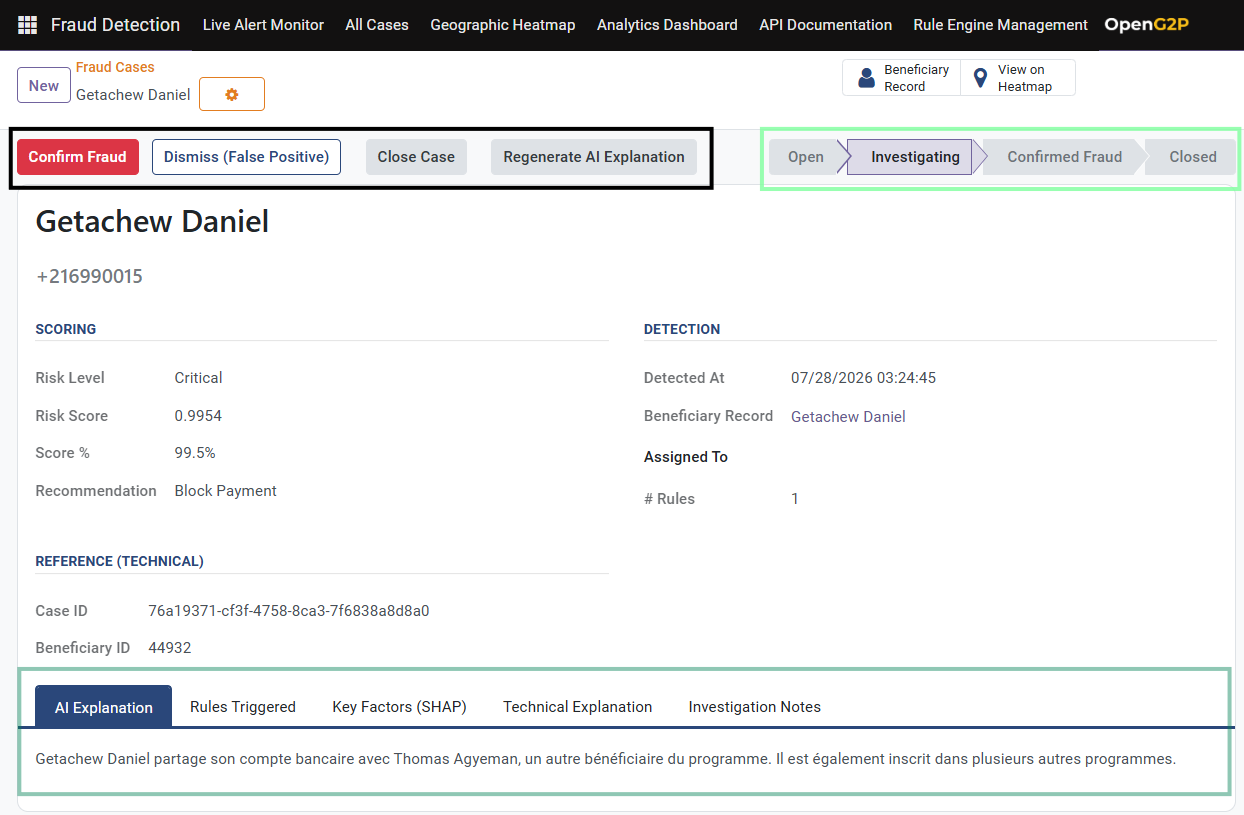
\includegraphics[width=\textwidth]{Dossier.png}
    \caption{Tableau de bord Odoo: outil de prise de décision  }
    \label{fig:odoo-case}
\end{figure}
\hspace{0.5cm}Chaque alerte critique est également enregistrée directement sur la fiche partenaire du bénéficiaire concerné (Figure~\ref{fig:odoo-partner-log}), sous forme de note horodatée dans le journal Odoo~: score, recommandation, règles déclenchées et identifiant du cas y figurent, avec la mention de l'engine ayant généré l'alerte. Cet historique cumulatif offre à l'analyste une vue immédiate de la récurrence des alertes pour un même bénéficiaire, sans quitter la fiche standard déjà utilisée pour la gestion des contacts dans OpenG2P.
\begin{figure}[H]
    \centering
    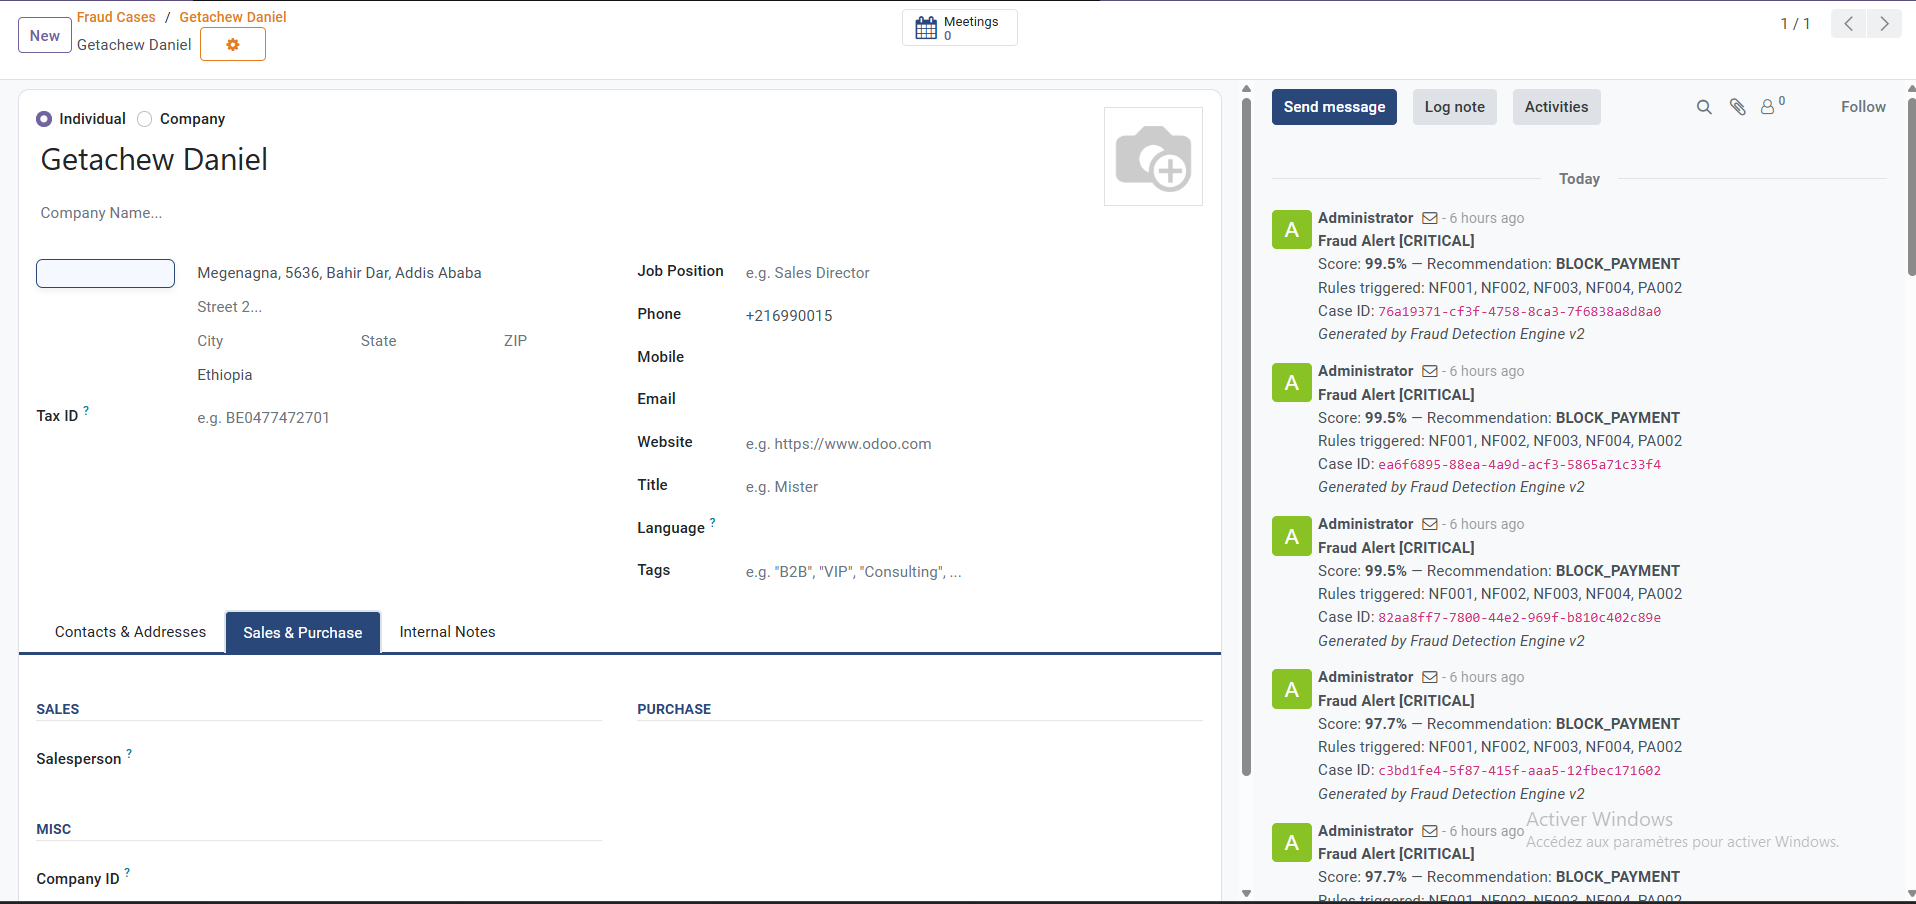
\includegraphics[width=0.92\textwidth]{Dossier2.png}
    \caption{Historique des alertes de fraude sur la fiche partenaire du bénéficiaire}
    \label{fig:odoo-partner-log}
\end{figure}

\subsection{Exposition via une API de services}

\hspace{0.5cm}L'ensemble du pipeline décrit précédemment est exposé sous forme de services accessibles à distance, ce qui permet à n'importe quel client — Odoo, tableau de bord, ou tout autre outil — de déclencher un scoring ou de consulter un cas sans connaître les détails d'implémentation du pipeline interne.

\begin{figure}[H]
    \centering
    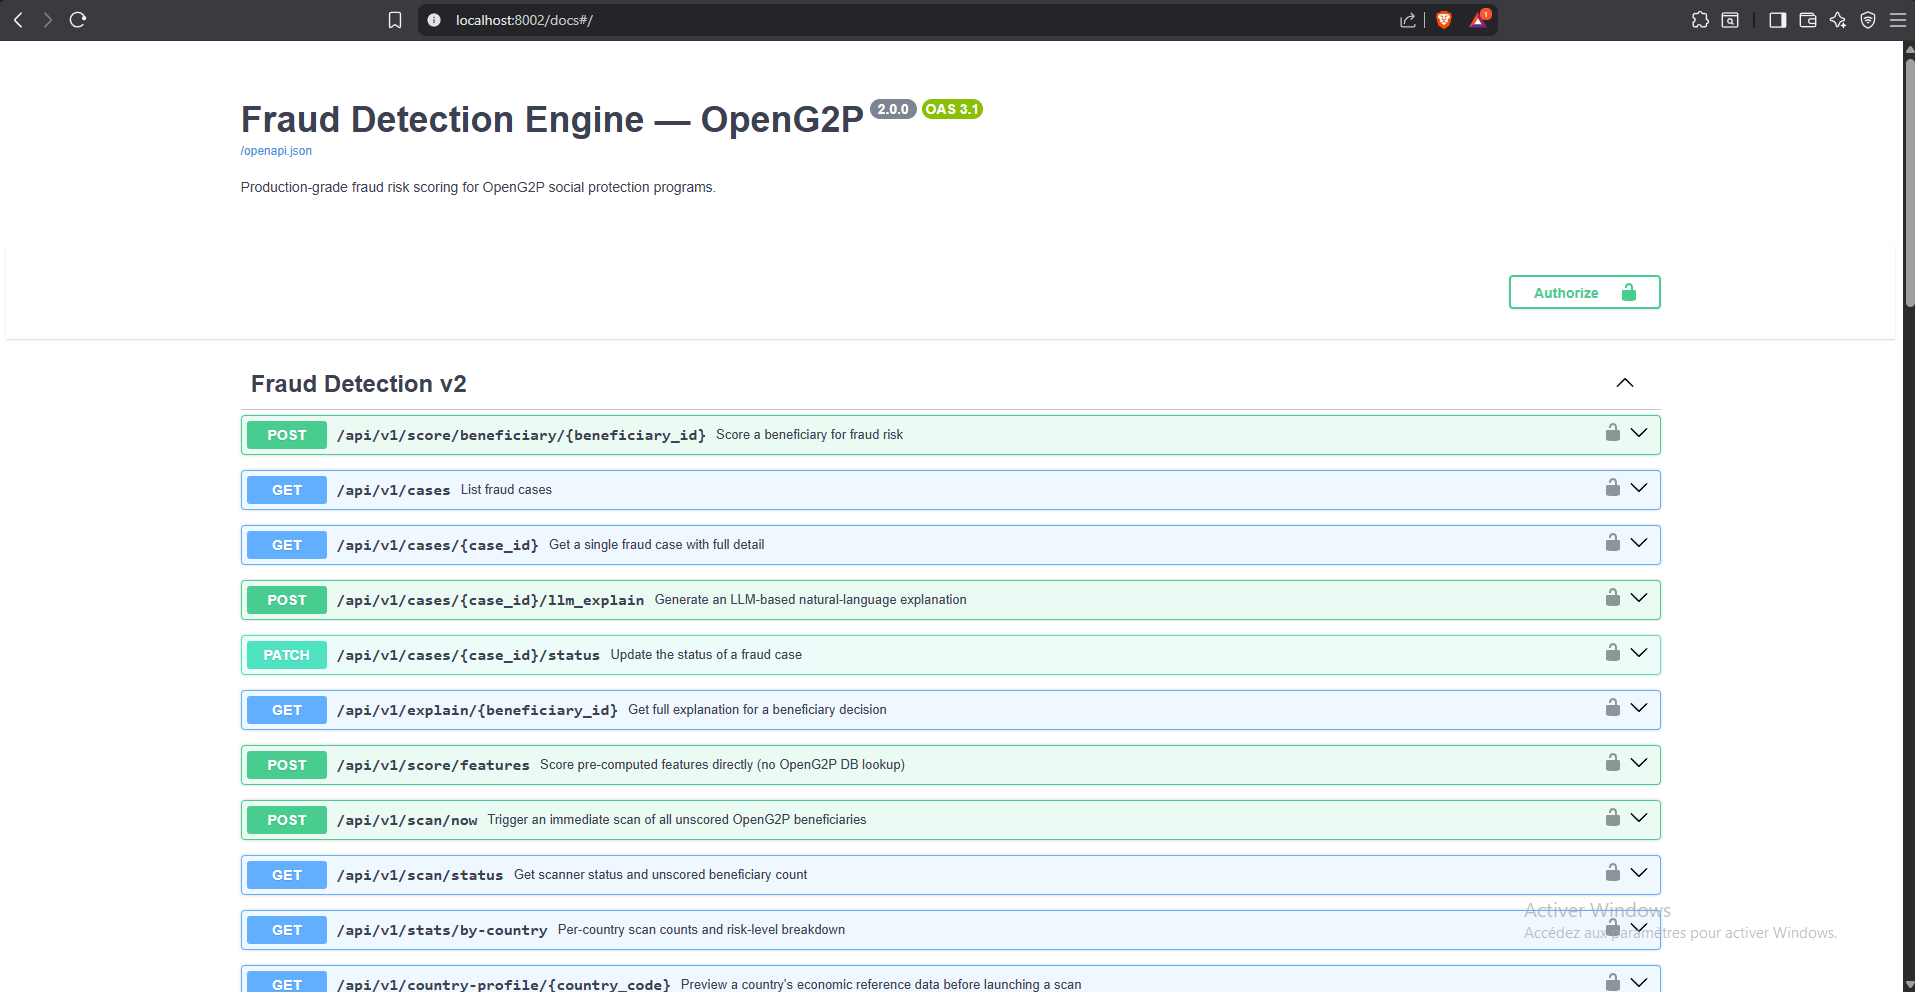
\includegraphics[width=\textwidth]{swagger.png}
    \caption{Documentation Swagger de l'API exposant le pipeline de scoring}
    \label{fig:swagger}
\end{figure}

\begin{figure}[H]
    \centering
    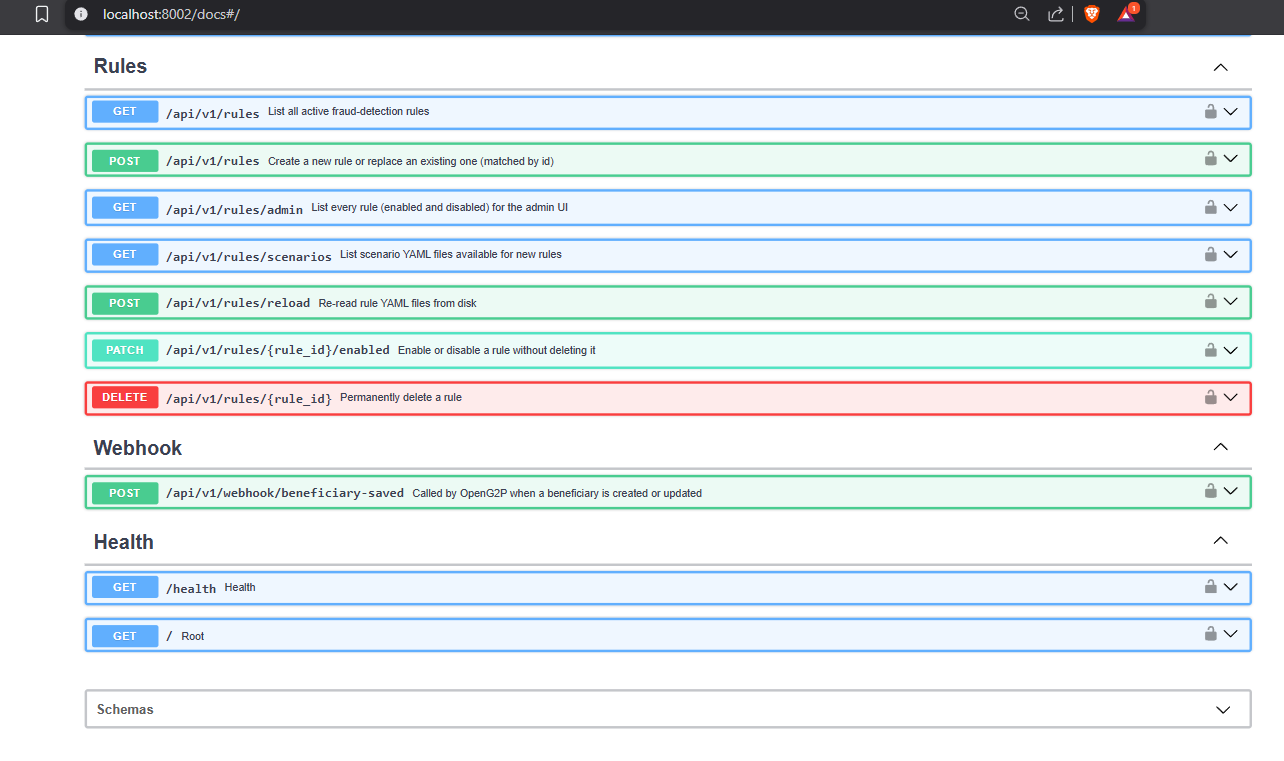
\includegraphics[width=\textwidth]{swagger2.png}
    \caption{Documentation Swagger de l'API exposant le pipeline de scoring}
    \label{fig:swagger-2}
\end{figure} 
\hspace{0.5cm}Les Figures~\ref{fig:swagger} et \ref{fig:swagger-2} présente la documentation interactive de l'API, générée automatiquement à partir du code selon le standard \textbf{OpenAPI 3.1}. Cette documentation reste toujours synchronisée avec l'implémentation réelle et permet de tester chaque endpoint directement depuis le navigateur. Les endpoints couvrent quatre besoins~: \textbf{scorer} un bénéficiaire (\texttt{POST /score/beneficiary/\{id\}}), \textbf{consulter} les cas de fraude (\texttt{GET /cases}), \textbf{générer une explication} (\texttt{POST /cases/\{id\}/llm\_explain}, \texttt{GET /explain/\{beneficiary\_id\}}), et \textbf{piloter} le scanner automatique (\texttt{POST /scan/now}).

\vspace{0.3cm}
{\large \textbf{Authentification et contrôle d'accès}}
\vspace{0.2cm}

\hspace{0.5cm}L'accès à l'API est protégé par authentification (bouton \textit{Authorize}, Figure~\ref{fig:swagger}), garantissant qu'aucun client non autorisé ne peut déclencher un scoring ou consulter un dossier de bénéficiaire. Ce contrôle d'accès s'appuie sur le système de groupes natif d'Odoo, avec trois rôles distincts~: \textbf{Agent Social}, qui peut consulter le statut d'un bénéficiaire sans accéder aux détails de scoring~; \textbf{Analyste Fraude}, qui dispose des droits complets sur les cas (investigation, confirmation, rejet, consultation des explications)~; et \textbf{Admin}, responsable de la configuration du moteur (gestion des règles, paramètres du scanner).

\begin{table}[H]
\centering
\caption{Rôles et permissions d'accès au système}
\label{tab:roles-access}
\renewcommand{\arraystretch}{1.4}
\begin{tabular}{>{\bfseries}p{2.8cm} p{9.5cm}}
\hline
\thead{Rôle} & \thead{Fonctionnalités accessibles} \\
\hline
\rowcolor{EYgray}
Agent Social & Consultation du statut d'un bénéficiaire, sans accès aux détails de scoring ni aux cas de fraude. \\
Analyste Fraude & Accès complet aux cas~: investigation, confirmation, rejet, consultation des explications (SHAP, LLM), historique des alertes. \\
\rowcolor{EYgray}
Admin & Configuration du moteur~: gestion des règles métier, paramètres du scanner, supervision globale du système. \\
\hline
\end{tabular}
\end{table}

\section{Tableau de bord de suivi - Streamlit}

\hspace{0.5cm}Le tableau de bord offre une vue consolidée des alertes en temps réel, complémentaire à l'intégration Odoo pour les usages d'analyse et de monitoring. Il comporte quatre volets~:

\begin{itemize}
    \item \textbf{Alertes actives}~: liste des bénéficiaires à risque critique ou élevé, avec filtre par programme, niveau de risque et date.
    \item \textbf{Graphe de réseau (Heatmap)}~: visualisation interactive du réseau de fraude, avec les communautés détectées mises en couleur.
    \item \textbf{Scoring Manuel d'un ou plusieurs bénéficiaires}~: permet de scorer manuellement un ou plusieurs bénéficiaires en saisissant leurs informations, et d'obtenir le score de risque ainsi que la recommandation correspondante.
    \item \textbf{Générateur d'explication par bénéficiaire}~: Générer des explications sur le niveau de risque d'un bénéficiaire donné.

\end{itemize}

\subsection{Tableau de bord de suivi du moteur de détection de fraude}
\hspace{0.5cm}Le tableau de bord (Figure~\ref{fig:dashboard}) permet aux analystes fraude de surveiller en temps réel les alertes générées par le moteur et de gérer les cas détectés. Les principales fonctionnalités sont résumées au Tableau~\ref{tab:dashboard-features}.
\begin{landscape}
\begin{figure}[H]
    \centering
    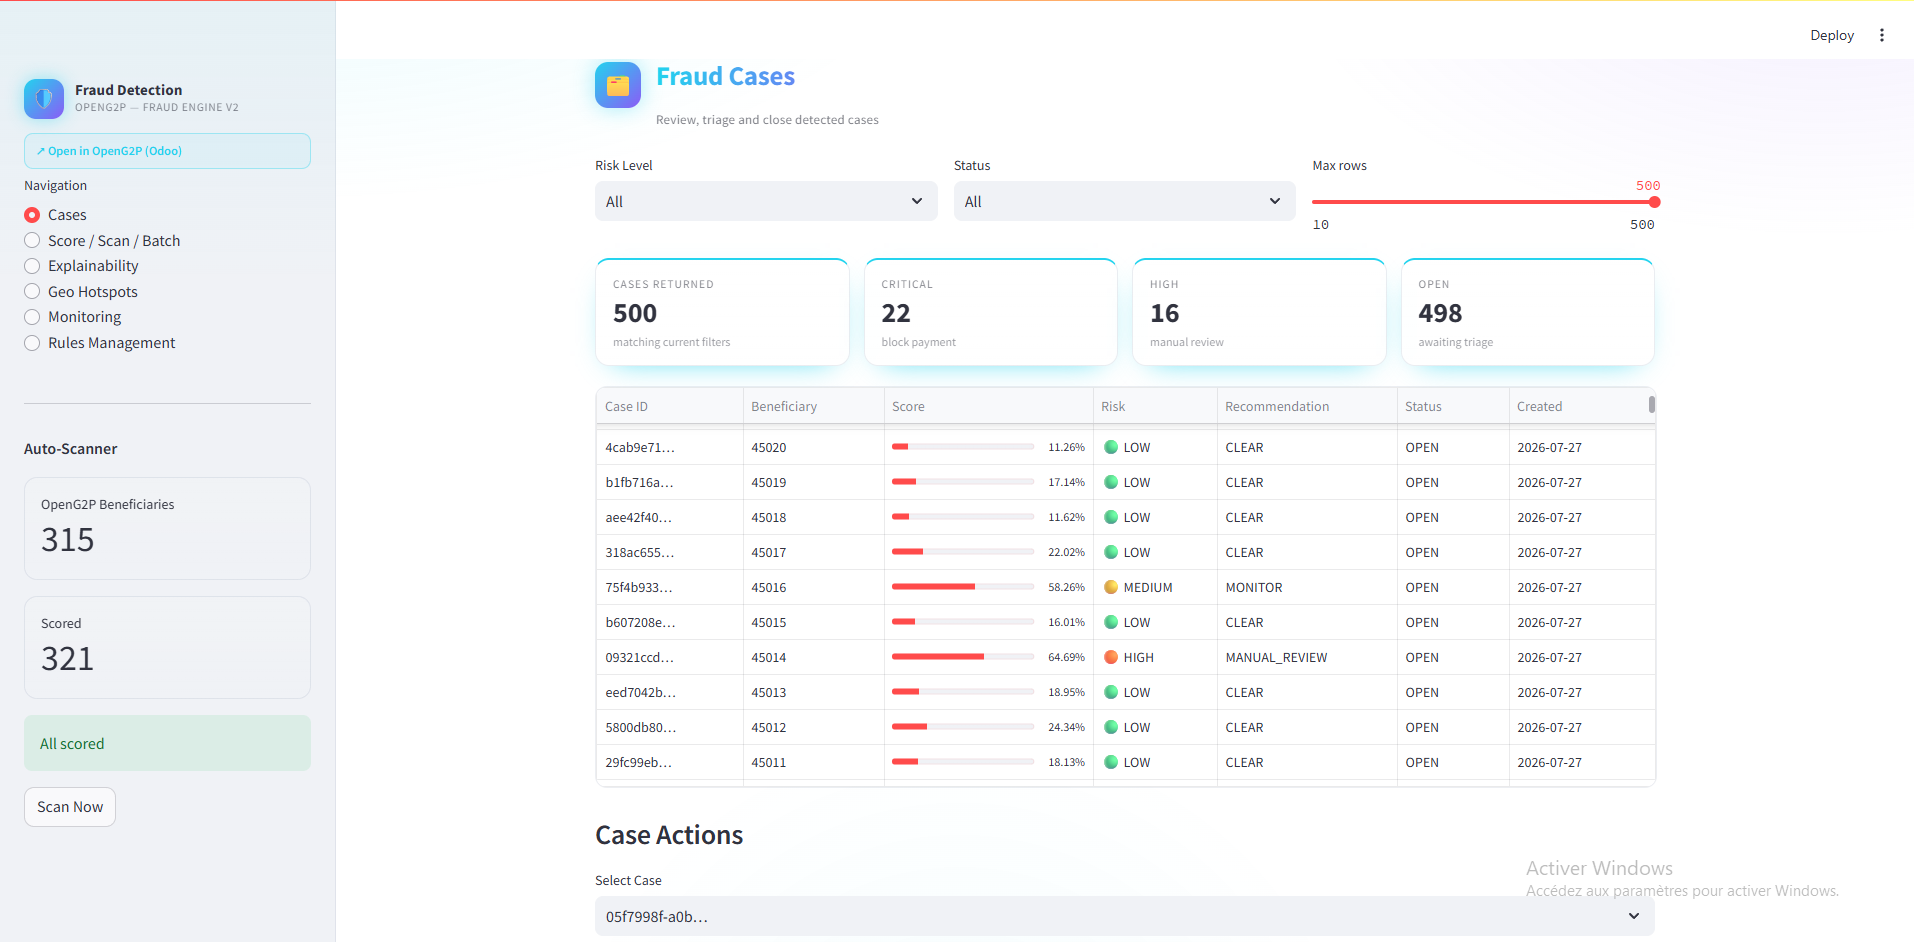
\includegraphics[width=1.4\textwidth]{Dashboard1.png}
    \caption{Tableau de bord de suivi des cas de fraude}
    \label{fig:dashboard}
\end{figure}
\end{landscape}

\begin{table}[H]
\centering
\caption{Fonctionnalités du tableau de bord pour l'analyste fraude}
\label{tab:dashboard-features}
\renewcommand{\arraystretch}{1.4}
\begin{tabular}{>{\bfseries}p{3cm} p{11cm}}
\hline
\thead{Section} & \thead{Fonctionnalité} \\
\hline
\rowcolor{EYgray}
\textbf{Fraud Cases} & Liste complète des bénéficiaires signalés, filtrage par niveau de risque (LOW, MEDIUM, HIGH, CRITICAL) et statut (OPEN, IN\_PROGRESS, RESOLVED). Affichage du score brut, de la recommandation (CLEAR, MONITOR, MANUAL\_REVIEW, BLOCK) et de la date de détection. \\
\textbf{Métriques} & Quatre cartes synthétiques~: cas retournés (matchant les filtres), cas CRITICAL (blocage paiement), cas HIGH (vérification manuelle), cas OPEN (en attente). Permet d'évaluer rapidement la charge de travail. \\
\rowcolor{EYgray}
\textbf{Auto-Scanner} & Affichage du nombre de bénéficiaires traités et du nombre restant. Bouton pour déclencher un scan immédiat sans attendre le cycle automatique. \\
\textbf{Case Actions} & Sélection d'un cas pour examiner son détail~: features brutes, facteurs SHAP, explication LLM. Mise à jour du statut et enregistrement de la décision finale de l'analyste. \\
\hline
\end{tabular}
\end{table}

\subsection{Analyse des dossiers de fraude}
\vspace{0.3cm}
\textbf{\large Analyse manuel d'un dossier}
\vspace{0.3cm}\newline
\begin{figure}[H]
    \centering
    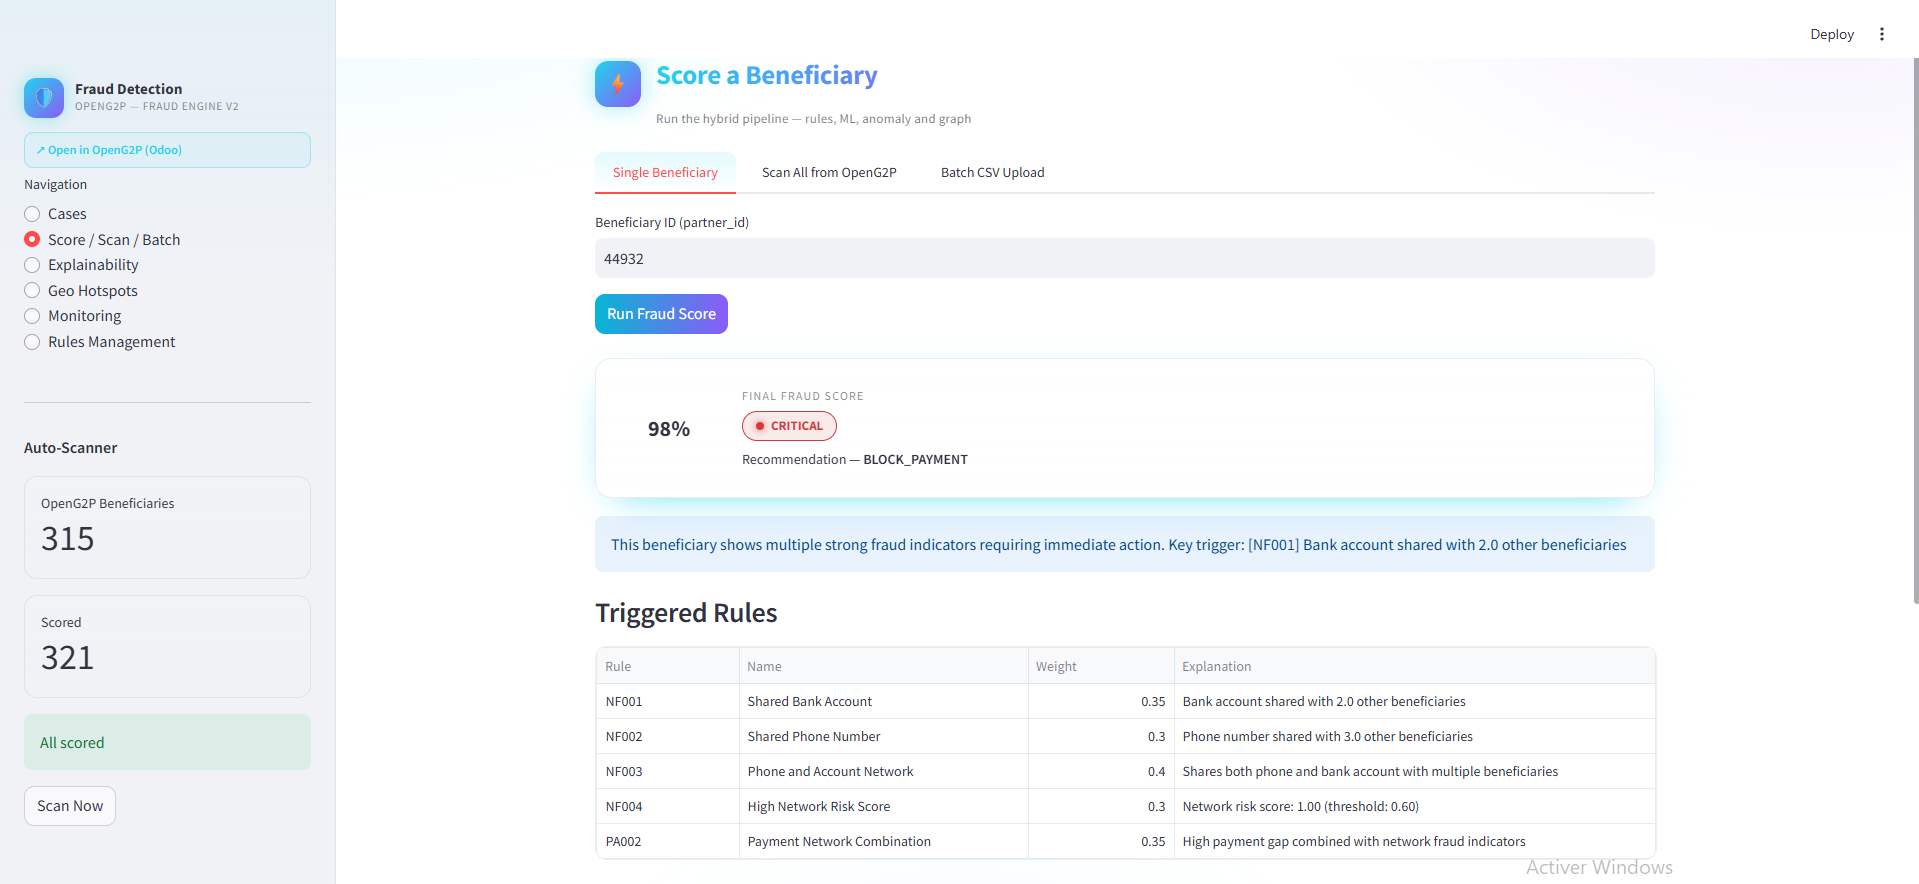
\includegraphics[width=\textwidth]{resultScoring.png}
    \caption{Résultat du scoring d'un bénéficiaire}
    \label{fig:result-scoring}
\end{figure}

\hspace{0.5cm}La Figure~\ref{fig:result-scoring} illustre le résultat du scoring d'un bénéficiaire, avec le score final, les signaux déclenchés, les facteurs SHAP et l'explication générée par le modèle de langage. L'analyste peut ainsi comprendre rapidement les raisons du signalement et décider des actions à entreprendre.
\newpage
\vspace{0.3cm}
\textbf{\large Analyse d'un lot de dossier}
\vspace{0.3cm}\newline
\begin{figure}[H]
    \centering
    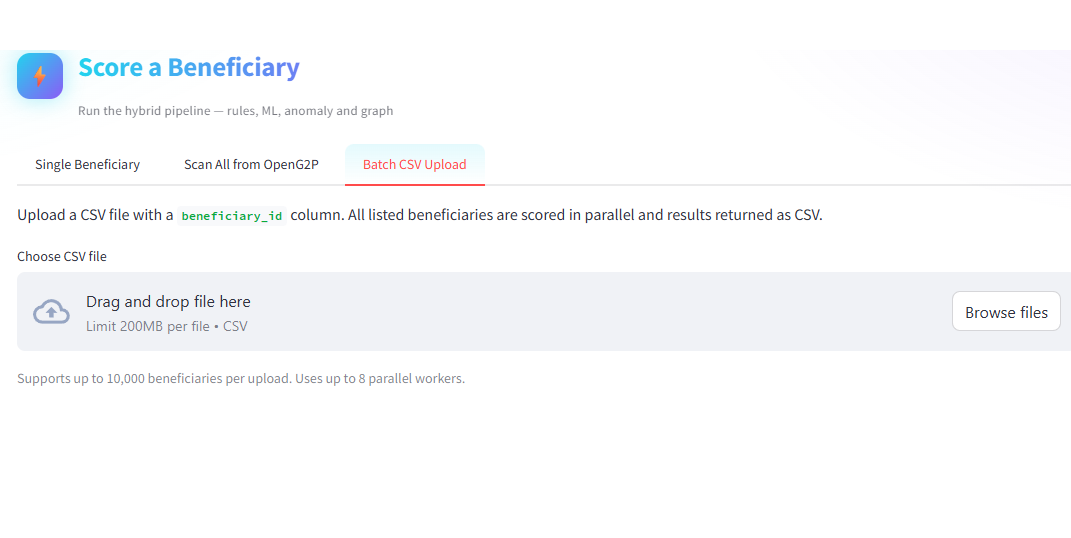
\includegraphics[width=\textwidth]{ScoreCSV.png}
    \caption{Scoring des bénéficiaire au format CSV}
    \label{fig:result-scoring-csv}
\end{figure}

\hspace{0.5cm}La Figure~\ref{fig:result-scoring-csv} illustre le scoring des bénéficiaires au format CSV, avec le score final, les signaux déclenchés, les facteurs SHAP et l'explication générée par le modèle de langage. L'analyste peut ainsi comprendre rapidement les raisons du signalement et décider des actions à entreprendre.

\vspace{0.3cm}
\textbf{\large Génération d'un rapport spécifique a un bénéficiaire}
\vspace{0.3cm}\newline
\hspace{0.5cm}L'analyste fraude peut générer un rapport PDF détaillé pour chaque cas signalé (Figure~\ref{fig:fraud-report}). Le rapport synthétise en une seule page~: l'identifiant du cas et du bénéficiaire, la date de génération, le statut de traitement, la recommandation du moteur (CLEAR, MONITOR, MANUAL\_REVIEW, BLOCK), et \textbf{le score final avec son niveau de risque} (LOW, MEDIUM, HIGH, CRITICAL).

\hspace{0.5cm}Le rapport inclut également un \textbf{diagramme de décomposition des scores}~: chaque composant (Rule Score, ML Score, Graph Score) y est visualisé, montrant sa contribution au score final. Les \textbf{cinq features les plus influentes} (selon SHAP) sont listées avec leur impact relatif, permettant à l'analyste de comprendre rapidement les raisons de l'alerte. Un tableau récapitulatif (Feature Vector) complète le rapport avec les 28 valeurs numériques brutes du bénéficiaire, garantissant la traçabilité complète de la décision.
\begin{figure}[H]
    \centering
    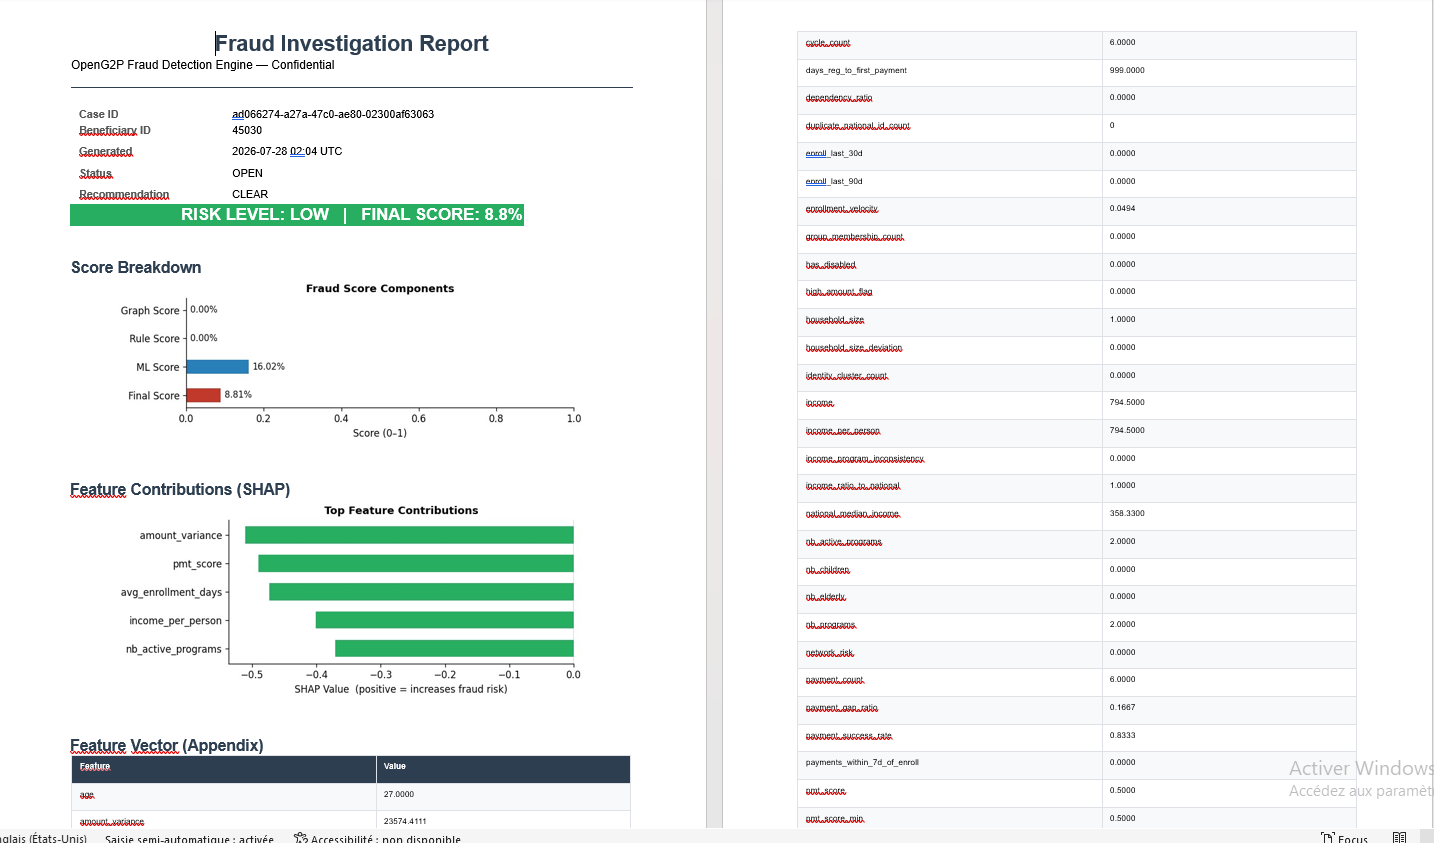
\includegraphics[width=\textwidth]{FraudReport.png}
    \caption{Génération de rapport de fraude d'un bénéficiaire}
    \label{fig:fraud-report}
\end{figure}

\vspace{0.3cm}
{\large \textbf{Génération d'une explication détaillée}}
\vspace{0.2cm}

\hspace{0.5cm}L'analyste fraude peut demander une explication complète sur chaque alerte~: quelles règles ont déclenché, les scores de chaque agent (ML, réseau, règles), et comment ils se combinent pour l'alerte finale (Figure~\ref{fig:explication}).

\begin{figure}[H]
    \centering
    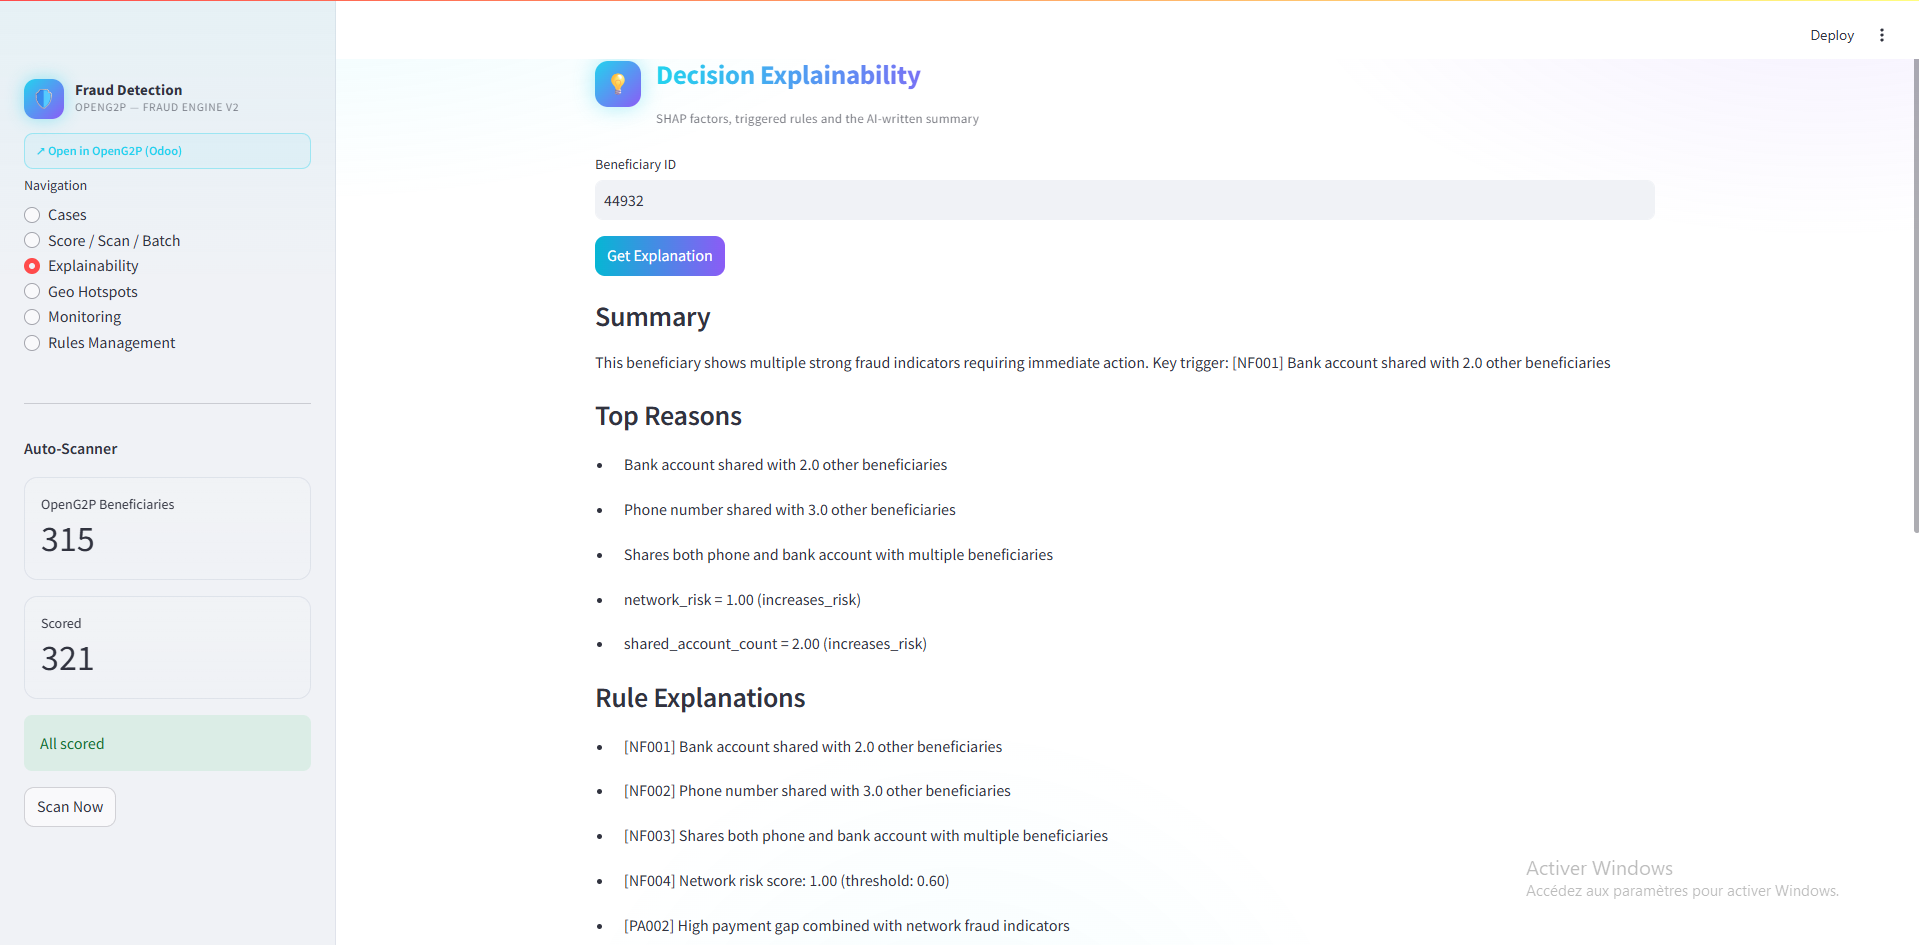
\includegraphics[width=0.92\textwidth]{explainability3.png}
    \caption{Explication détaillée d'une décision de fraude}
    \label{fig:explication}
\end{figure}
\newpage
\vspace{0.2cm}
{\large \textbf{Analyse géospatiale des fraudes}}
\vspace{0.3cm}

\hspace{0.5cm}Au-delà du scoring individuel, le système détecte également les \textbf{fraudes organisées par zone géographique}. L'algorithme DBSCAN regroupe les bénéficiaires spatialement proches(en fonction des adresses ou des zones fournies lors de l'inscription au programme social) dont les scores de fraude sont élevés, révélant des poches de fraude concentrées. La Figure~\ref{fig:geohotspots} cartographie ces clusters~: les zones en rouge et orange signalent une densité de fraude importante (West Africa notamment), tandis que les zones vertes indiquent des clusters isolés de faible densité. Cette vue permet aux équipes d'ajuster les contrôles par région~: renforcer les vérifications manuelles dans les zones critiques, ou adapter les seuils de risque selon le contexte géographique du programme.

\hspace{0.5cm}Le tableau joint synthétise les onze clusters détectés~: pour chacun, on retrouve le centre géographique (latitude/longitude), le rayon englobant les bénéficiaires du cluster, le nombre total de cas, le nombre de cas HIGH ou CRITICAL, le taux de fraude moyen, et le score moyen. Le cluster 6 (Senegal/Guinea-Bissau) concentre 11 cas HIGH ou CRITICAL sur 27 bénéficiaires (taux de fraude de 40,7~%), marquant le foyer prioritaire d'investigation.

\begin{figure}[H]
    \centering
    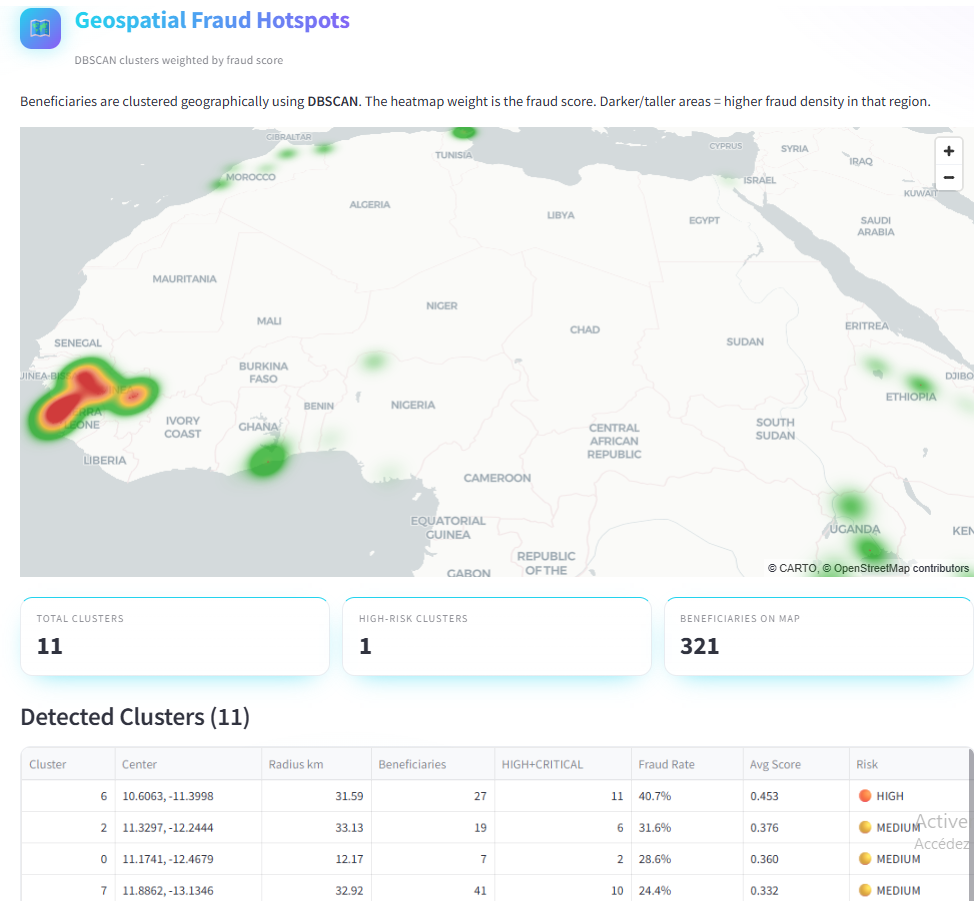
\includegraphics[width=0.92\textwidth]{GeoHotspot.png}
    \caption{Carte des clusters de fraude géographiques détectés par DBSCAN}
    \label{fig:geohotspots}
\end{figure}

    \vspace{0.3cm}
    
{\large \textbf{Monitoring et amélioration continue du système}}
\vspace{0.2cm}

\hspace{0.5cm}Un tableau de bord dédié (Figure~\ref{fig:monitoring}) permet de superviser la santé du moteur en temps réel~: statut du service, disponibilité des modèles ML, nombre de règles actives. La distribution des risques affiche le nombre de cas par niveau (LOW, MEDIUM, HIGH, CRITICAL) et par recommandation (CLEAR, MONITOR, MANUAL\_REVIEW, BLOCK\_PAYMENT), donnant une vue instantanée de la charge d'investigation.

\hspace{0.5cm}Une section \textbf{Investigator Feedback} collecte les retours des analystes~: nombre de verdicts confirmés, fraudes validées, faux positifs détectés. Ces données alimentent automatiquement un cycle de réentraînement hebdomadaire~: les cas confirmés comme frauduleux et les faux positifs servent de labels pour affiner les modèles ML, garantissant que le système s'adapte aux patterns de fraude émergents et réduit progressivement ses erreurs.

\begin{figure}[H]
    \centering
    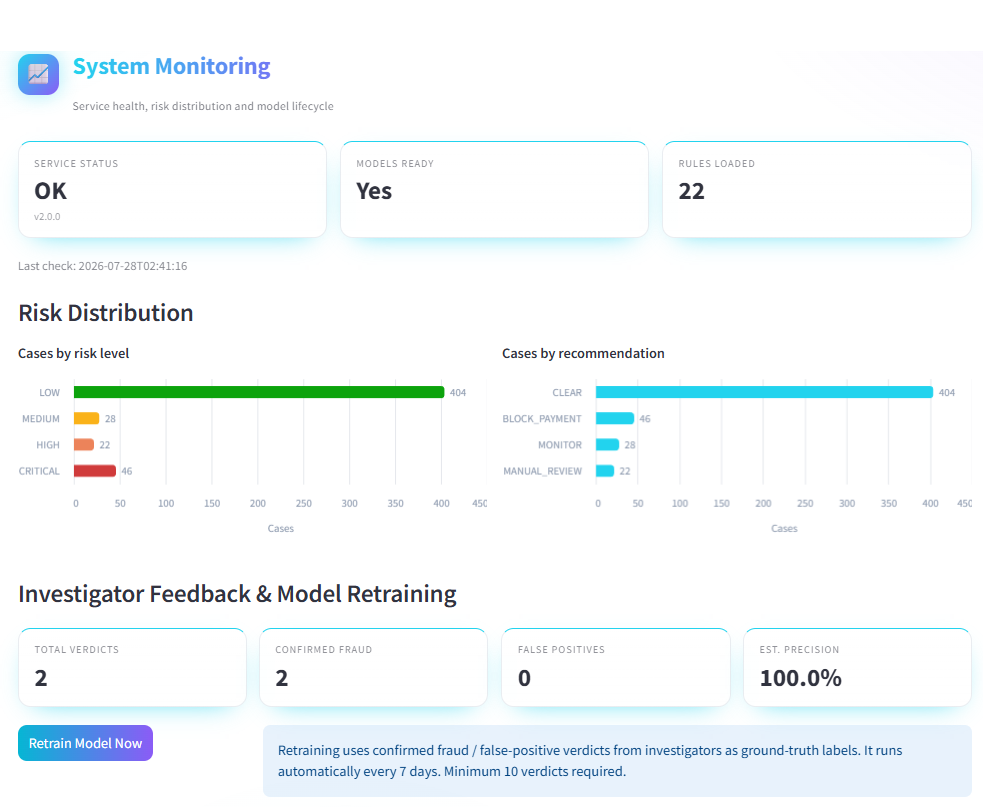
\includegraphics[width=0.92\textwidth]{monitoring.png}
    \caption{Tableau de monitoring du système et feedback des analystes}
    \label{fig:monitoring}
\end{figure}

\newpage
\vspace{0.3cm}
{\large \textbf{Gestion des règles métier}}
\vspace{0.2cm}

\hspace{0.5cm}Un interface dédié (Figure~\ref{fig:rules-management}) permet aux administrateurs de créer, modifier ou désactiver les règles de détection sans redémarrer le service. Les règles sont stockées en YAML et rechargées automatiquement après chaque modification. Les conditions sont évaluées via un évaluateur AST restreint (opérations arithmétiques et comparaisons uniquement), ce qui garantit la sécurité~: aucun code Python arbitraire ne peut être injecté.


\begin{figure}[H]
    \centering
    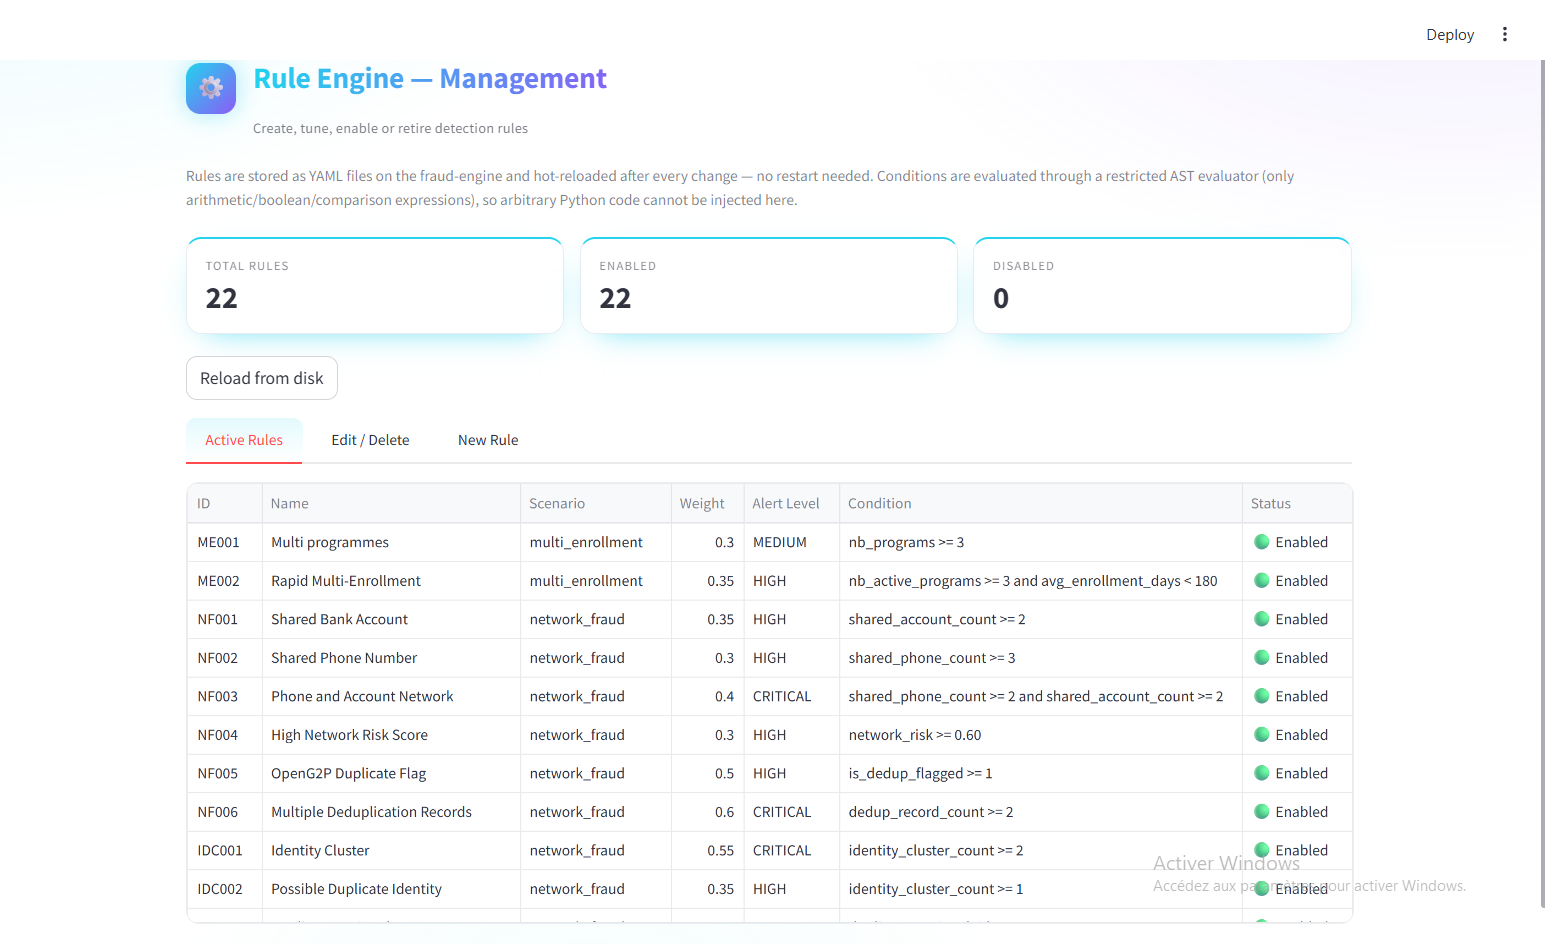
\includegraphics[width=0.92\textwidth]{rulesmanagement.png}
    \caption{Interface de gestion des règles de détection de fraude}
    \label{fig:rules-management}
\end{figure}

\hspace{0.5cm}Le tableau affiche les 22 règles actives avec leur identifiant, nom, scénario de fraude couvert (multi-enrollment, network\_fraud, duplicate identity), poids dans le score final, niveau d'alerte déclenché, et condition logique. Chaque règle peut être activée, modifiée ou supprimée indépendamment, offrant une flexibilité maximale aux métiers pour adapter la détection sans intervention technique.

\section{Conclusion partielle}
% ─────────────────────────────────────────────────────────────

\hspace{0.5cm}Ce chapitre a présenté la mise en œuvre complète du moteur intelligent, depuis la génération des données d'entraînement jusqu'au déploiement de l'interface utilisateur. Toutes les fonctionnalités spécifiées au chapitre précédent ont été réalisées et intégrées dans un système cohérent et déployable via une seule commande Docker Compose.

\textbf{Récapitulatif des fonctionnalités développées~:}

\begin{itemize}
    \item Génération d'un dataset synthétique de 5~000 bénéficiaires (13,2~\% de fraudes, 9 scénarios) avec injection PostgreSQL
    \item Extraction de 28 features SQL multi-tables depuis OpenG2P avec gestion défensive des valeurs manquantes
    \item Moteur de règles métier~: 22 règles YAML réparties en 5 scénarios, évaluation sécurisée par AST, \texttt{rule\_score} avec liste de signaux déclenchés
    \item Ensemble par stacking (Random Forest, XGBoost, Régression Logistique + méta-modèle) avec correction du déséquilibre par pondération de classe (\texttt{class\_weight}, \texttt{scale\_pos\_weight})~: AUC~0,912, F1~0,748 au seuil retenu
    \item Isolation Forest pour la détection d'anomalies non supervisée, exposée dans l'explicabilité (intégration au score pondéré final~: piste d'amélioration, voir dernier chapitre)
    \item Graphe NetworkX + PageRank pour l'identification des réseaux frauduleux
    \item Score hybride pondéré (20~\% règles + 55~\% ML + 25~\% graphe) avec 4 niveaux de risque
    \item Explicabilité SHAP (importance globale et individuelle) + LLM Mistral via Ollama (explication en français naturel)
    \item Module Odoo \texttt{g2p\_fraud\_detection} avec synchronisation automatique et webhook de scoring en temps réel
    \item Tableau de bord de suivi~: dossiers de fraude, métriques synthétiques, auto-scanner, actions sur les cas
\end{itemize}

\hspace{0.5cm}Le chapitre suivant évalue la performance de ce système dans des conditions proches de la production : métriques ML approfondies, tests d'intégration avec OpenG2P, analyse des cas limites et mesure des temps de réponse.

\chapter{Perspectives}

\hspace{0.5cm}Le moteur présenté dans ce mémoire est fonctionnel~: il extrait les données d'OpenG2P, calcule un score hybride, l'explique et restitue une décision dans l'interface des agents sociaux. Il reste néanmoins un prototype validé en environnement de développement. Ce chapitre revient d'abord sur ses limites, puis expose les évolutions envisagées à court terme, les conditions d'un passage en production, et enfin les extensions possibles au-delà du cadre initial.

\section{Limites du travail réalisé}

\hspace{0.5cm}La principale limite tient à la nature des données. Faute d'accès à un registre social réel — les données de bénéficiaires étant sensibles et protégées — l'entraînement repose sur un jeu synthétique généré à partir de distributions plausibles. Le recours au dataset PaySim a permis de vérifier que la chaîne d'entraînement généralise à des données réelles, mais rien ne garantit que les fraudeurs réels d'un programme de protection sociale se comportent exactement comme ceux du générateur. Les métriques obtenues doivent donc se lire comme une validation de la méthode, non comme une prédiction de performance en conditions réelles.

\hspace{0.5cm}Deux autres limites méritent d'être signalées. Les poids de la formule hybride ont été fixés par raisonnement sur la nature de chaque signal, non appris sur des données de validation. Et le système n'a jamais été confronté à des analystes fraude en situation réelle~: son ergonomie et la pertinence de ses explications restent à valider auprès des utilisateurs finaux.

\section{Améliorations à court terme}

\subsection{Apprentissage des poids de fusion}

\hspace{0.5cm}Les poids 55/20/25 pourraient être estimés statistiquement plutôt que fixés a priori. La méthodologie de Noçairi et al.~\cite{nocairi2016stacking}, déjà mobilisée pour justifier la combinaison pondérée, propose d'apprendre ces poids par régression logistique PLS sur les prédictions validées croisées — une approche qui garantit leur positivité et leur optimalité au sens d'un critère de performance mesurable. Cette évolution suppose de disposer d'un volume suffisant de verdicts d'analystes pour servir de vérité terrain.

\subsection{Intégration du score d'anomalie}

\hspace{0.5cm}L'Isolation Forest est aujourd'hui calculé et affiché, mais exclu du score de décision. Son intégration avec un poids faible — de l'ordre de 5~\% — donnerait au système un filet de sécurité contre les fraudes émergentes, celles dont aucun exemple ne figure encore dans les données d'entraînement. Ce poids devra être réévalué conjointement aux trois autres.

\subsection{Calibration par pays}

\hspace{0.5cm}Les seuils des règles métier sont actuellement identiques pour tous les contextes. Or un revenu de 800~unités monétaires n'a pas la même signification selon le revenu médian national. Le raccordement à l'API de la Banque Mondiale permettrait de calibrer automatiquement ces seuils sur des indicateurs locaux (revenu médian, seuil de pauvreté, taille moyenne des ménages), avec une table de référence pré-alimentée pour garantir des évaluations déterministes et rapides.

\subsection{Enrichissement des explications par RAG}

\hspace{0.5cm}Les explications générées par Mistral s'appuient aujourd'hui sur les seuls facteurs SHAP du cas courant. Une base vectorielle ChromaDB contenant des cas de fraude historiques documentés permettrait au modèle de langage de s'appuyer sur des précédents comparables, rendant l'explication plus concrète pour l'analyste. Cet usage reste strictement narratif~: les seuils numériques continuent de provenir du moteur de règles, jamais de la base vectorielle.

\section{Conditions d'un déploiement réel}

\subsection{Protection des données personnelles}

\hspace{0.5cm}Un déploiement sur données réelles impose un cadre juridique et technique que le prototype n'aborde pas. Le système manipule des données personnelles sensibles — revenus, composition du ménage, handicap, coordonnées bancaires — soumises aux réglementations nationales de protection des données. Trois chantiers en découlent~: la minimisation des données extraites, la traçabilité des accès (qui a consulté quel dossier, quand), et le droit du bénéficiaire à contester une décision automatisée. Ce dernier point rejoint directement le travail sur l'explicabilité~: une explication compréhensible n'est pas seulement un confort pour l'analyste, elle devient une obligation.

\subsection{Supervision du modèle en production}

\hspace{0.5cm}Un modèle entraîné une fois se dégrade avec le temps~: les profils de bénéficiaires évoluent, et les fraudeurs s'adaptent aux contrôles. La boucle de réentraînement déjà en place — alimentée par les verdicts des investigateurs — constitue une première réponse, mais elle suppose un volume régulier de retours et un suivi de la dérive des distributions. Un système d'alerte sur la dérive des features, comparant les distributions courantes à celles de l'entraînement, permettrait de déclencher un réentraînement avant que les performances ne se dégradent visiblement.

\subsection{Montée en charge}

\hspace{0.5cm}Le prototype traite quelques centaines de bénéficiaires. Un programme national en compte des centaines de milliers, voire des millions. Deux composants demandent une attention particulière à cette échelle~: la construction du graphe relationnel, dont le coût croît fortement avec le nombre de nœuds et d'arêtes, et la génération d'explications par le modèle de langage, coûteuse en temps de calcul. Une stratégie de traitement par lots, un calcul incrémental du graphe, et une génération d'explication à la demande — plutôt que systématique — constituent les pistes les plus immédiates.

\section{Extensions envisageables}

\hspace{0.5cm}Au-delà du programme initial, le moteur est conçu pour être réutilisable. Les règles métier étant externalisées en fichiers de configuration et modifiables sans redéploiement, l'adaptation à un autre programme social — pension de vieillesse, allocation scolaire, aide alimentaire — relève d'un travail de paramétrage plutôt que de développement. La même logique vaut pour un déploiement dans un autre pays~: la calibration par indicateurs nationaux, décrite plus haut, en constitue le prérequis technique.

\hspace{0.5cm}À plus long terme, le système peut être envisagé comme une brique d'infrastructure publique numérique, greffable sur n'importe quelle plateforme de transferts sociaux exposant ses données. L'architecture en services, découplée de l'implémentation interne du pipeline, a été pensée dans cette optique~: un client qui consomme l'API n'a pas besoin de connaître les modèles utilisés, ni leur nombre.

\hspace{0.5cm}Enfin, une dimension reste largement inexplorée~: l'usage du moteur non pour sanctionner, mais pour corriger. Les mêmes signaux qui détectent la fraude peuvent révéler des erreurs d'inclusion involontaires — un ménage mal enregistré, un revenu saisi dans la mauvaise unité — et servir à améliorer la qualité du registre social plutôt qu'à exclure des bénéficiaires. Cette réorientation, plus qu'une évolution technique, relève d'un choix de conception que le système actuel rend déjà possible.











%═════════════════════════════════════════════════
% SECTION RÉFÉRENCES (à inclure dans votre biblio)
% ═════════════════════════════════════════════════
 
\begin{thebibliography}{99}
 
\bibitem{BM_PovertyData2023}
Banque Mondiale. (2023). \textit{World Development Indicators}. 
\url{https://data.worldbank.org/indicator}

\bibitem{OpenG2P_Docs2023}
OpenG2P Community. (2023). \textit{OpenG2P Technical Documentation and Deployment Guide}.
\url{https://openg2p.dev/docs/}

\bibitem{BM_Sourcebook2020}
Banque Mondiale. (2020). \textit{The Sourcebook of Social Protection Programmes}.
Chapter 8: Social Protection Finance and Risk. Washington, DC.

\bibitem{Nocairi2016}
Noçairi, H., Gomes, C., Thomas, M., \& Saporta, G. (2016).
\textit{Improving Stacking Methodology for Combining Classifiers: Applications to Cosmetic Industry}.
Electronic Journal of Applied Statistical Analysis, 9(2), 340--361.
\url{https://doi.org/10.1285/i20705948v9n2p340}

\end{thebibliography}

\end{document}
